\documentclass[10pt,a4paper]{article}
\AtBeginDocument{\fontsize{14pt}{17pt}\selectfont}
\usepackage[a4paper,margin=1.5cm]{geometry}  % comfortable page margins
\usepackage{microtype}                       % improved character spacing/justification
\usepackage{enumitem}                        % fine-grained list control

%% fix mathbb font for digits
\DeclareMathAlphabet{\mathbb}{U}{bbold}{m}{n}
\usepackage{amsmath,amssymb,amsthm,booktabs}
\usepackage{tikz}
\usetikzlibrary{arrows.meta,decorations.markings,calc,patterns,positioning,shapes.geometric}
\usepackage{caption}
\usepackage[T1]{fontenc}
\usepackage{lmodern}
\usepackage{microtype}
\usepackage[colorlinks=true,linkcolor=blue,citecolor=blue]{hyperref}

\theoremstyle{remark}
\newtheorem*{remark}{Remark}
\newtheorem*{warning}{Caution}

\newcommand{\dbar}{\mathchar'26\mkern-11mu d}
\newcommand{\Var}{\operatorname{Var}}
\newcommand{\Cov}{\operatorname{Cov}}
\newcommand{\Tr}{\operatorname{Tr}}

\title{Thermodynamic Potentials, Ensembles, and Heat Capacity\\
\large A working guide for condensed-matter graduate students}
\author{}
\date{}

\begin{document}
\maketitle

\begin{abstract}
These notes assemble the machinery that connects a statistical ensemble to a
measurable response function. The logical chain is: (i) the fundamental relation
$U(S,V,N)$ encodes everything; (ii) Legendre transforms trade a variable for its
conjugate and produce the \emph{thermodynamic potentials}, each of which is
minimised at equilibrium under the constraints appropriate to it; (iii) each
ensemble computes one such potential as the logarithm of a partition function;
(iv) second derivatives of that potential are response functions, and by the
fluctuation--dissipation structure of the ensemble they equal variances of the
fluctuating quantities. Particular attention is paid to several points that are
routinely glossed over: the precise status and logical origin of $\dbar Q =
T\,dS$, the difference between the Legendre transform and the variational
principle it is often conflated with, and the fact that the constant-$\mu$ and
constant-$N$ heat capacities are not the same function. A final strand runs the
argument backwards: because a phase transition exists only in the thermodynamic
limit, no finite simulation can display one, and Section~\ref{sec:fss} develops
finite-size scaling from its assumptions --- turning that obstruction into the
measuring instrument --- together with a conventional Monte Carlo protocol for
extracting critical exponents from it accurately.
\end{abstract}

\tableofcontents

\section{Notation and conventions}
\label{sec:notation}

$k_B$ is Boltzmann's constant and $\beta = 1/k_BT$. We write $\dbar Q$ and
$\dbar W$ (rather than $dQ$, $dW$) for inexact differentials, i.e.\ small
quantities that are \emph{not} the differential of any state function. Work is
counted positive when done \emph{on} the system, so $\dbar W = -P\,dV$ for
reversible compression.

Several notational hazards are worth flagging immediately, because they are a
source of much confusion in the literature. First, $\Omega$ is used both for the grand
potential and for the microcanonical multiplicity. In these notes $\Omega$
\emph{always} means the grand potential, and the number of accessible microstates
is written $W(E,V,N)$. Second, $\Delta$ is standard both for the \emph{gap
exponent} of critical phenomena (Section~\ref{sec:criticalnonanalytic}) and for
the isothermal--isobaric partition function (Section~\ref{sec:ensembles}); the two
never appear in the same formula, and each is redefined where it is used. Two
further collisions are unavoidable if standard notation is to be kept, and are
resolved by context: $\omega$ is the grand potential density $\Omega/V$, a
measurement frequency in $c(\omega)$, and the leading correction-to-scaling
exponent of Section~\ref{sec:fss}; and $\beta$ is the inverse temperature
$1/k_BT$ everywhere except in lists of critical exponents, where it is the
order-parameter exponent $m\sim|t|^{\beta}$. Where the latter could be genuinely
ambiguous --- in the Monte Carlo protocol of
Section~\ref{sec:fss:implementation} --- the inverse temperature is written out or
carried as the coupling $K=J/k_BT$.

\section{The fundamental thermodynamic relation}

For a simple compressible system with variable particle number, all equilibrium
information is contained in a single function,
\[
U = U(S,V,N).
\]

\paragraph{What to call $U$.} Three names are in circulation for the same symbol
and they are not interchangeable, so it is worth fixing the usage before it
causes trouble.

\begin{itemize}
\item \textbf{Internal energy} names the \emph{physical quantity}: the total
energy content of the system, exclusive of its bulk kinetic and potential energy.
This is the correct name for $U$ in every context and in every set of variables,
and it is the one to use when in doubt. It is a state function, so $U$ has the
same value at a given equilibrium state no matter which variables one chooses to
label that state with.
\item \textbf{Fundamental relation} names the \emph{particular functional form}
$U(S,V,N)$ --- the internal energy expressed in its natural, entirely extensive
variables. The adjective is Callen's and it is earned: $U(S,V,N)$ contains
strictly more information than $U$ expressed in terms of, say, $(T,V,N)$, in the
precise sense established in Section~\ref{sec:legendre}. So ``the fundamental
relation'' is a statement about \emph{which variables} $U$ is a function of, not
about $U$ itself. The entropy representation $S(U,V,N)$, obtained by solving for
$S$, is an equally fundamental relation and carries exactly the same information.
\item \textbf{Thermodynamic potential} is the generic term for any member of the
family $\{U,H,F,G,\Omega\}$ of Section~\ref{sec:potentials}: functions whose
first derivatives return the conjugate variables, which are related to one
another by Legendre transformation, and each of which is minimised at equilibrium
under its own constraints. $U$ is a member of that family --- indeed the
generating member --- so calling it a thermodynamic potential is correct but
uninformative, since it does not say \emph{which} potential. Note that some
authors restrict the term to the \emph{transformed} potentials and thereby exclude
$U$; and ``free energy'' is never used for $U$, being reserved for $F$ and $G$.
\end{itemize}

The convention adopted here is the usual one: $U$ is called the internal energy
throughout; the phrase \emph{fundamental relation} refers specifically to the
function $U(S,V,N)$ in its natural variables; and \emph{potential} is used
collectively when a statement applies to the whole family.

The total differential is
\[
dU=
\left(\frac{\partial U}{\partial S}\right)_{V,N}dS+
\left(\frac{\partial U}{\partial V}\right)_{S,N}dV+
\left(\frac{\partial U}{\partial N}\right)_{S,V}dN,
\]
and the partial derivatives \emph{define} the conjugate intensive variables
\[
T\equiv\left(\frac{\partial U}{\partial S}\right)_{V,N},\qquad
-P\equiv\left(\frac{\partial U}{\partial V}\right)_{S,N},\qquad
\mu\equiv\left(\frac{\partial U}{\partial N}\right)_{S,V},
\]
giving
\[
\boxed{\;dU=T\,dS-P\,dV+\mu\,dN\;}
\]
The three terms are the thermal, mechanical, and chemical channels through which
energy enters. In a condensed-matter setting $-P\,dV$ generalises to
$\sum_{ij}V\sigma_{ij}\,d\epsilon_{ij}$ for elastic strain, to $\mathbf{H}\cdot
d\mathbf{M}$ for magnetic work, to $\mathbf{E}\cdot d\mathbf{P}$ for dielectric
work, and so on; everything below goes through with $(-P,V)$ replaced by the
relevant conjugate pair.

\subsection{On what grounds may \texorpdfstring{$dU$}{dU} be expanded in \texorpdfstring{$dS$, $dV$, $dN$}{dS, dV, dN}?}
\label{sec:totaldiff}

The expansion written above looks like a triviality of multivariable calculus. It
is not. It encodes four separate assumptions --- one empirical, three structural
--- and each of them fails somewhere in condensed matter. They are worth
separating, because each failure is a distinct physical situation with a distinct
remedy, and because the list makes clear exactly what has to be true of a material
before the boxed relation may be written down at all.

\paragraph{(A1) $U$ is a single-valued function of state.} This is empirical
content, not mathematics. Its basis is Joule's observation that the work required
to carry an adiabatically enclosed system from one state to another is
path-independent; that path-independence is what permits $U$ to be defined, up to
an additive constant, as a function on the space of equilibrium states. Where it
fails, it fails badly: a ferromagnet driven around a hysteresis loop returns to
the same $(T,H)$ with a different magnetisation and a different internal energy.
There is then no function $U$ of those variables to differentiate, and every
equation in this section is void before it starts.

\paragraph{(A2) The list of variables is complete --- the state postulate.} We
assume that an equilibrium state of a simple, one-component, single-phase system
is fixed by $(S,V,N)$ and nothing else, so the state space is a three-dimensional
manifold. The count is: one thermal coordinate, plus one coordinate per
independent work mode, plus one per chemical species. Adding a work mode adds a
coordinate and a term, which is why the magnetic, elastic, and interfacial
generalisations quoted above are extensions of the state space rather than
rewritings of it.

The deeper content of the state postulate is a statement about \emph{timescale
separation}, and one must be careful about \emph{which} timescales, because the
usual one-line version invites a fair objection. Every thermodynamic variable is
a macroscopic average over $\sim10^{23}$ microscopic degrees of freedom; if the
system is in equilibrium at all, then $T$, $P$, $\mu$, $S$, $V$, $N$ are sharp
numbers with relative fluctuations of order $N^{-1/2}$, and it is meaningless to
say that any of \emph{them} has a relaxation time comparable to the measurement.
That objection is correct. The resolution is that promoting an extra coordinate
is a statement about \emph{equilibration}, not about fluctuation: the added
variable is itself a macroscopic, sharply defined average, and what distinguishes
it is only that it has not yet reached the value that minimises the free energy.

Let $\tau_{\rm fast}$ be the relaxation time of the microscopic degrees of freedom
(electron and phonon collision times, $10^{-13}$--$10^{-11}\,\mathrm{s}$); let
$\xi$ be a \emph{macroscopic}, coarse-grained collective variable --- an order
parameter, the extent of a chemical reaction, a configurational coordinate in a
glass --- with its own relaxation time $\tau_\xi\gg\tau_{\rm fast}$; and let
$\tau_{\rm obs}$ be the duration of the measurement. Three regimes must be
distinguished, and only the middle one adds a coordinate.

\begin{itemize}
\item $\tau_\xi\ll\tau_{\rm obs}$: \textbf{$\xi$ is equilibrated.} Its value is
already a function of $(S,V,N)$, fixed by the condition $\mathcal{A}=0$ below. It
is not an independent coordinate, and the state postulate stands exactly as
written. All the internal variables of an ordinary simple fluid are of this type,
which is why $(S,V,N)$ suffices.

\item $\tau_\xi\gg\tau_{\rm obs}$: \textbf{$\xi$ is frozen, and must be promoted.}
It holds one definite macroscopic value throughout the measurement --- but not the
equilibrium value. Every fast degree of freedom has nevertheless equilibrated
\emph{at that fixed} $\xi$, so $T$, $P$, and $\mu$ are as well defined and as
sharp as ever; the system sits in \emph{constrained} equilibrium. Nothing has
started fluctuating; what has happened is that the equilibrium manifold acquired
an extra label, and the state space is genuinely four-dimensional:
\[
U=U(S,V,N;\xi),\qquad
dU=T\,dS-P\,dV+\mu\,dN-\mathcal{A}\,d\xi ,
\qquad
\mathcal{A}\equiv-\left(\frac{\partial U}{\partial\xi}\right)_{S,V,N} ,
\]
with $\mathcal{A}$ the affinity conjugate to $\xi$. Physical instances: a glass
quenched below $T_g$, whose configurational coordinate is fixed at the value it
had when it fell out of equilibrium; an alloy with a frozen long-range order
parameter; the ortho/para ratio in solid hydrogen, which relaxes over days.
Because $\xi$ is off its equilibrium value, $\mathcal{A}\neq0$, and any residual
drift of $\xi$ produces entropy at the rate
$T\,d\sigma=\mathcal{A}\,d\xi\geq0$. This is the formal home of the irreversible
quasi-static processes catalogued in Section~\ref{sec:clausius}.

\item $\tau_\xi\sim\tau_{\rm obs}$: \textbf{no state description at all.} Here
$\xi$ neither tracks the constraints nor holds still, and there is no equilibrium
manifold --- however enlarged --- on which to define $U$. State functions must be
given up in favour of frequency-dependent response, $c(\omega)=c'(\omega)-i
c''(\omega)$ (Section~\ref{sec:clausius}). So a relaxation time
\emph{comparable} to the measurement is precisely the regime in which no
coordinate can be assigned; a relaxation time \emph{long} compared with the
measurement is the regime in which one is added. The original slogan conflates
the two, and only the second is a statement about state space.
\end{itemize}

The correct coordinates are therefore the slow variables --- typically the
conserved densities, whose relaxation time diverges with system size as
$\tau\sim L^{2}/D$ --- \emph{together with} any variable frozen on the timescale
of observation, under the assumption that everything else has equilibrated. All
of them are macroscopic averages with negligible relative fluctuations. It is
their \emph{number}, not their sharpness, that the state postulate is about.

\paragraph{(A3) The variables are independent.} The symbol $(\partial U/\partial
S)_{V,N}$ presupposes that $S$ can be varied while $V$ and $N$ are held fixed.
Formally, $(S,V,N)$ must constitute a \emph{coordinate chart}: the three functions
must be functionally independent, so that $\{dS,dV,dN\}$ is a basis of the
cotangent space and the coefficients in the expansion are unique.

This is not automatic, and thermodynamics supplies its own counterexample. The
intensive triple $(T,P,\mu)$ is \emph{not} independent: Gibbs--Duhem,
\[
S\,dT-V\,dP+N\,d\mu=0,
\]
is exactly a functional dependence among them. One therefore may not expand any
quantity in $dT$, $dP$, and $d\mu$ simultaneously --- the three coordinate
one-forms are linearly dependent at every point, and the would-be expansion
coefficients are not unique. This is the precise reason the ``fourth'' Legendre
transform $U-TS+PV-\mu N$ vanishes identically rather than yielding a new
potential. The extensive variables escape this because they can be independently
prescribed by physical operations --- wall off a volume, admit particles, add
heat --- whereas the intensive ones are already derivatives of the fundamental
relation and inherit relations among themselves.

\paragraph{(A4) $U$ is continuously differentiable, not merely equipped with
partial derivatives.} This is the assumption most often passed over in silence,
and it is strictly stronger than it looks. The equation
\[
dU=\sum_i\left(\frac{\partial U}{\partial x_i}\right)dx_i
\]
asserts that the increment is captured by a \emph{linear} map,
\[
U(\mathbf{x}+\mathbf{h})-U(\mathbf{x})=\sum_i a_ih_i+o(|\mathbf{h}|),
\]
which is the definition of (total, Fr\'echet)
differentiability.\footnote{\label{fn:landau}\textbf{Landau symbols.} Let
$g(\mathbf{h})>0$ (here $g=|\mathbf{h}|$) and let $\mathbf{h}\to0$. Then
$r=O(g)$, ``at most of order $g$'', means $|r|\leq Cg$ for some constant $C$ and
all small $|\mathbf{h}|$: an upper bound, nothing more. $r=o(g)$, ``of smaller
order than $g$'', means $r/g\to0$; equivalently, for \emph{every} $\epsilon>0$ one
has $|r|\leq\epsilon g$ for all sufficiently small $|\mathbf{h}|$. And
$r=\Theta(g)$, ``exactly of order $g$'', means $c\,g\leq|r|\leq Cg$ for constants
$0<c\leq C$: upper \emph{and} lower bounds, so $r/g$ neither diverges nor tends to
zero. The relations among them are $o(g)\subset O(g)$ and $\Theta(g)\subset O(g)$,
but crucially $\Theta(g)\cap o(g)=\emptyset$ --- a remainder cannot be both exactly
of order $g$ and of smaller order than $g$ --- and it is this disjointness that
does the work in the text. With $g=|h|$ in one variable: $h^{2}=o(|h|)$;
$3h=\Theta(|h|)$, hence $O(|h|)$ but not $o(|h|)$; $|h|^{3/2}=o(|h|)$; and
$h\sin(1/h)=O(|h|)$ but is neither $o(|h|)$ (the ratio oscillates) nor
$\Theta(|h|)$ (it vanishes at $h=1/n\pi$). In more than one variable the constants
must be uniform in the direction of approach, and it is exactly that uniformity
clause which fails below.} Mere existence
of the partial derivatives does not deliver it. Consider
\[
f(x,y)=\frac{x^{3}}{x^{2}+y^{2}},\qquad f(0,0)=0 .
\]
In polar form $f=r\cos^{3}\theta$, so $f$ is continuous everywhere; both partial
derivatives exist everywhere, with $f_x(0,0)=1$ and $f_y(0,0)=0$. Yet the
proposed linear approximation fails at the origin:
\[
r(h,k)\;\equiv\;f(h,k)-\big[f(0,0)+1\cdot h+0\cdot k\big]
=-\frac{hk^{2}}{h^{2}+k^{2}} .
\]
Differentiability demands $r(\mathbf{h})=o(|\mathbf{h}|)$, i.e.\ that the
\emph{ratio} $r(\mathbf{h})/|\mathbf{h}|$ tend to zero. It does not. Along the
line $h=k$ we have $r=-h/2$ while $|\mathbf{h}|=\sqrt{2}\,|h|$, so
\[
\frac{r(\mathbf{h})}{|\mathbf{h}|}\;=\;\frac{-h/2}{\sqrt{2}\,|h|}
\;=\;\mp\frac{1}{2\sqrt{2}}\qquad(h\to0^{\pm}),
\]
a nonzero constant.

\paragraph{The same statement without any asymptotic notation.} The content of
the example is easier to see, and easier to state correctly, in terms of
directional derivatives. Along the ray $\mathbf{h}=t\,\hat{\mathbf{u}}$ with
$\hat{\mathbf{u}}=(\cos\theta,\sin\theta)$,
\[
f(t\cos\theta,\,t\sin\theta)=\frac{t^{3}\cos^{3}\theta}{t^{2}}=t\cos^{3}\theta
\qquad\Longrightarrow\qquad
D_{\hat{\mathbf{u}}}f(0)=\cos^{3}\theta .
\]
So every directional derivative exists; there is nothing pathological about the
individual limits. But if $f$ were differentiable at the origin, with gradient
$\nabla f=(f_x,f_y)=(1,0)$, the directional derivative would have to be the
\emph{linear} function of direction
\[
\nabla f\cdot\hat{\mathbf{u}}=\cos\theta ,
\]
and $\cos^{3}\theta\neq\cos\theta$.

That is the whole failure, and it is worth putting in exactly the right words.
The trouble is \emph{not} that the derivative depends on the direction: for every
non-constant differentiable function it does, through $\nabla
f\cdot\hat{\mathbf{u}}$, and a direction-independent derivative would be a very
strange thing to demand. The trouble is that it depends on direction
\emph{non-linearly}. Differentiability is precisely the assertion that the map
$\hat{\mathbf{u}}\mapsto D_{\hat{\mathbf{u}}}f$ is linear --- equivalently, that it
is given by contraction with a single covector, which is the content of
Section~\ref{sec:totaldiff}'s geometric restatement. A function whose directional
derivatives fail to be linear in the direction has no gradient, no differential,
and no tangent plane, however many directional derivatives exist individually.

The two descriptions are the same calculation. Along the ray,
$r(t\hat{\mathbf{u}})=f(t\hat{\mathbf{u}})-f(0)-t\,\nabla
f\cdot\hat{\mathbf{u}}=t\big(D_{\hat{\mathbf{u}}}f-\nabla
f\cdot\hat{\mathbf{u}}\big)+o(t)$, so
\[
\frac{r(\mathbf{h})}{|\mathbf{h}|}\;\xrightarrow[t\to0^{+}]{}\;
D_{\hat{\mathbf{u}}}f-\nabla f\cdot\hat{\mathbf{u}}
=\cos^{3}\theta-\cos\theta=-\cos\theta\,\sin^{2}\theta ,
\]
which at $\theta=45^{\circ}$ equals $-1/(2\sqrt{2})$ --- exactly the constant
found above along $h=k$. The remainder fails to be $o(|\mathbf{h}|)$ in a given
direction by precisely the amount by which $D_{\hat{\mathbf{u}}}f$ fails to be
linear in $\hat{\mathbf{u}}$.

One caution on the notation, since the Landau symbols are easy to misuse
(footnote~\ref{fn:landau}): observing that $r=O(|\mathbf{h}|)$ settles nothing on
its own, because $o(|\mathbf{h}|)\subset O(|\mathbf{h}|)$ --- every admissible
remainder is also $O(|\mathbf{h}|)$. What excludes differentiability is that $r$
is $\Theta(|\mathbf{h}|)$ along some direction; the \emph{lower} bound is the
operative half. The culprit is visible in $f_x$,
which tends to $1$ along $y=0$ and to $0$ along $x=0$: the partials exist but are
discontinuous, so $f$ is not
$C^{1}$.\footnote{\label{fn:Cn}\textbf{Differentiability classes.} For an open
set $\mathcal{O}\subseteq\mathbb{R}^{m}$, a function $f:\mathcal{O}\to\mathbb{R}$
is of class $C^{n}$ ($n=0,1,2,\dots$) if all its partial derivatives up to and
including order $n$ exist at every point of $\mathcal{O}$ and are continuous
there; $C^{0}$ is thus continuity alone and $C^{\infty}$ means $C^{n}$ for every
$n$. The classes are strictly nested, $C^{\infty}\subset\cdots\subset
C^{2}\subset C^{1}\subset C^{0}$, and each inclusion is proper: $|x|$ is $C^{0}$
but not $C^{1}$, and $x|x|$ is $C^{1}$ but not $C^{2}$. On a manifold the same
definition is applied in any chart; because the transition maps between charts of
a $C^{\infty}$ atlas are themselves $C^{\infty}$, the class of $f$ does not depend
on which chart is used. Two facts are used repeatedly below: $f\in C^{1}$ implies
$f$ is (totally, Fr\'echet) differentiable, so $df$ exists as a one-form; and
$f\in C^{2}$ implies the Hessian is symmetric, which is what makes the Maxwell
relations of Section~\ref{sec:exact} available. Note also that $C^{\infty}$ is
still weaker than \emph{analytic}: $e^{-1/t^{2}}$ is $C^{\infty}$ at $t=0$ yet has
identically vanishing Taylor series there.}

The sufficient condition is the familiar one: if the partials exist in a
neighbourhood and are continuous there, then $f$ is $C^{1}$ and the expansion is
valid. Translated into physics, the requirement is that
\[
T,\quad -P,\quad \mu \qquad\text{be \emph{continuous} functions of state,}
\]
since they \emph{are} the partial derivatives. Assumption (A4) is thus not an
analyst's fussiness but a physical condition on the equation of state.

\subsubsection*{Where (A4) fails --- and, importantly, where it does not}

The energy representation is remarkably robust here, and the contrast with the
Legendre-transformed potentials is instructive.

At a first-order transition the two phases satisfy the coexistence conditions
\[
T_\ell=T_g\equiv T_t,\qquad P_\ell=P_g\equiv P_t,\qquad \mu_\ell=\mu_g\equiv\mu_t ,
\]
which are just the statement that heat, volume, and particles have nothing further
to gain by moving from one phase to the other (Figure~\ref{fig:firstorder}a). Read
as a statement about the \emph{function} $U(S,V,N)$, these three equalities say
that its three first partial derivatives take the \emph{same} values on either
side of the transition. The first derivatives of $U$ are therefore continuous
there, and $U$ is $C^{1}$ across the transition. Nothing in
$dU=T\,dS-P\,dV+\mu\,dN$ is in trouble.

What \emph{does} happen is that $S$ and $V$ jump --- by the latent heat
$\Delta S=L/T_t$ and by the volume change $\Delta V$ --- while the intensive
variables do not. Geometrically this means the following. Fix $N$, and fix a
temperature $T_t$ on the coexistence curve. The set of two-phase states at that
temperature is the straight segment, the \emph{tie line}, joining
$(S_\ell,V_\ell)$ to $(S_g,V_g)$ in the $(S,V)$ plane: a mixture with liquid
fraction $x$ has
\[
S=xS_\ell+(1-x)S_g,\qquad V=xV_\ell+(1-x)V_g,\qquad
U=xU_\ell+(1-x)U_g ,
\]
all three interpolating linearly in the \emph{same} parameter $x$ (this is the
lever rule; it neglects the interface, which costs $O(L^{d-1})$ and is
subextensive). Eliminating $x$ shows that $U$ is an \emph{affine} function of
$(S,V)$ along each tie line, so the two-phase part of the $U$ surface is swept out
by straight segments as $T_t$ runs along the coexistence curve. It is a
\emph{ruled} surface: perfectly flat along each tie line, curved transverse to
them.

Parametrise a tie line by $\lambda$, with $\lambda=0$ at the liquid end and
$\lambda=1$ at the gas end, and extend the straight line beyond both ends into the
single-phase regions (Figure~\ref{fig:firstorder}b). Then $U(\lambda)$ is convex
and curved for $\lambda<0$, exactly straight on $[0,1]$, and convex and curved
again for $\lambda>1$. On the straight piece $T$ and $P$ are \emph{constant} ---
constant, note, not discontinuous --- because they are the slopes of an affine
function; and their constant values are exactly the single-phase slopes at the two
endpoints, because the endpoints are single-phase states. So the flat piece joins
the curved pieces with a common tangent. That is all that ``the tangent plane is
shared by the two phases'' means, and it is the double-tangent construction of
Section~\ref{sec:maxwell} read in the energy representation.

What $U$ loses is therefore not differentiability but \emph{strict} convexity. A
convex function that is affine on a segment is still $C^{1}$ --- the slope is
continuous, it simply stops changing --- but its second derivative vanishes on the
segment and jumps at the endpoints, so $U$ is $C^{1}$ and not
$C^{2}$.\footnote{See footnote~\ref{fn:Cn} for the classes $C^{n}$.} Since $C_V$,
$\kappa_T$, and every other response function is built from \emph{second}
derivatives, they are what misbehave; the one-form $dU$ is untouched. This is the
content of Section~\ref{sec:maxwell}, not a failure of the total differential:
\[
dU=T\,dS-P\,dV+\mu\,dN \qquad\text{survives a first-order transition intact.}
\]

\begin{figure}[htbp]
\centering
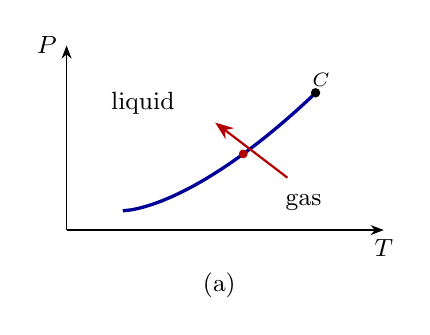
\begin{tikzpicture}[>=Stealth,font=\small,x=1.02cm,y=0.70cm]
  \draw[->] (0,0) -- (3.95,0) node[below]{$T$};
  \draw[->] (0,0) -- (0,3.35) node[left]{$P$};
  \draw[very thick,blue!60!black,domain=0.7:3.1,smooth,variable=\x]
       plot ({\x},{0.35+0.55*pow(\x-0.7,1.55)});
  \fill (3.1,2.49) circle (1.7pt);
  \node[anchor=south west,inner sep=1pt,font=\scriptsize] at (3.02,2.55) {$C$};
  \node at (0.95,2.30) {liquid};
  \node at (2.95,0.50) {gas};
  \draw[->,thick,red!70!black] (2.75,0.95) -- (1.85,1.95);
  \fill[red!70!black] (2.2,1.381) circle (1.6pt);
  \node[anchor=north,font=\small] at (1.9,-0.60) {(a)};
\end{tikzpicture}
\hfill
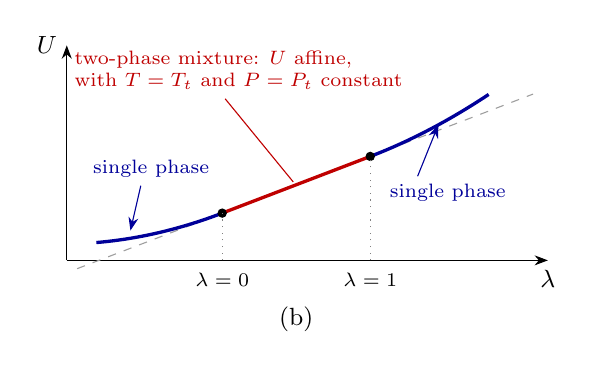
\begin{tikzpicture}[>=Stealth,font=\small,x=1.88cm,y=0.60cm]
  \draw[->] (-1.05,0) -- (2.20,0) node[below]{$\lambda$};
  \draw[->] (-1.05,0) -- (-1.05,4.55) node[left]{$U$};
  \draw[dashed,gray!75] (-0.98,-0.176) -- (2.10,3.520);
  \draw[very thick,blue!60!black,domain=-0.85:0,smooth,variable=\x]
       plot ({\x},{1.0+1.2*\x+0.55*\x*\x});
  \draw[very thick,red!75!black] (0,1.0) -- (1,2.2);
  \draw[very thick,blue!60!black,domain=1:1.80,smooth,variable=\x]
       plot ({\x},{1.0+1.2*\x+0.55*(\x-1)*(\x-1)});
  \fill (0,1.0) circle (1.7pt);
  \fill (1,2.2) circle (1.7pt);
  \draw[dotted,gray] (0,0) -- (0,1.0);
  \draw[dotted,gray] (1,0) -- (1,2.2);
  \node[anchor=north,font=\scriptsize] at (0,-0.06) {$\lambda=0$};
  \node[anchor=north,font=\scriptsize] at (1,-0.06) {$\lambda=1$};
  \node[anchor=north west,font=\scriptsize,red!75!black,align=left,inner sep=1pt]
       at (-1.02,4.50) {two-phase mixture: $U$ affine,\\ with $T=T_t$ and $P=P_t$ constant};
  \draw[red!75!black,thin] (0.02,3.42) -- (0.48,1.66);
  \node[anchor=south,font=\scriptsize,blue!60!black,inner sep=1.5pt] at (-0.48,1.65)
       {single phase};
  \draw[->,blue!60!black,thin] (-0.55,1.58) -- (-0.62,0.63);
  \node[anchor=north west,font=\scriptsize,blue!60!black,inner sep=1.5pt] at (1.10,1.72)
       {single phase};
  \draw[->,blue!60!black,thin] (1.32,1.78) -- (1.46,2.87);
  \node[anchor=north,font=\small] at (0.5,-0.78) {(b)};
\end{tikzpicture}

\vspace{1.5ex}
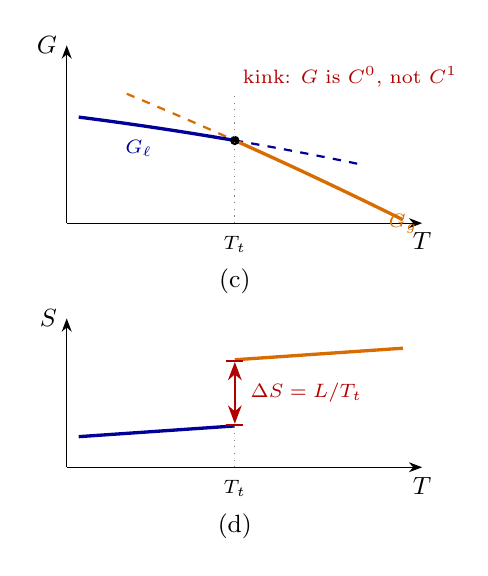
\begin{tikzpicture}[>=Stealth,font=\small,x=3.05cm,y=1.05cm]
  \draw[->] (0.30,0) -- (1.78,0) node[below]{$T$};
  \draw[->] (0.30,0) -- (0.30,2.15) node[left]{$G$};
  \draw[thick,orange!85!black,dashed,domain=0.55:1,smooth,variable=\x]
       plot ({\x},{1.0-1.3*(\x-1)-0.10*(\x-1)*(\x-1)});
  \draw[thick,blue!60!black,dashed,domain=1:1.52,smooth,variable=\x]
       plot ({\x},{1.0-0.5*(\x-1)-0.10*(\x-1)*(\x-1)});
  \draw[very thick,blue!60!black,domain=0.35:1,smooth,variable=\x]
       plot ({\x},{1.0-0.5*(\x-1)-0.10*(\x-1)*(\x-1)});
  \draw[very thick,orange!85!black,domain=1:1.70,smooth,variable=\x]
       plot ({\x},{1.0-1.3*(\x-1)-0.10*(\x-1)*(\x-1)});
  \fill (1,1.0) circle (1.7pt);
  \draw[dotted,gray] (1,0) -- (1,1.55);
  \node[anchor=north,font=\scriptsize] at (1,-0.04) {$T_t$};
  \node[anchor=north,font=\scriptsize,blue!60!black] at (0.60,1.12) {$G_\ell$};
  \node[anchor=north west,font=\scriptsize,orange!85!black] at (1.60,0.22) {$G_g$};
  \node[anchor=south west,font=\scriptsize,red!70!black,inner sep=1pt]
       at (1.02,1.60) {kink: $G$ is $C^{0}$, not $C^{1}$};
  \node[anchor=north,font=\small] at (1.0,-0.44) {(c)};
  \begin{scope}[yshift=-3.10cm]
    \draw[->] (0.30,0) -- (1.78,0) node[below]{$T$};
    \draw[->] (0.30,0) -- (0.30,1.80) node[left]{$S$};
    \draw[very thick,blue!60!black] (0.35,0.37) -- (1,0.5);
    \draw[very thick,orange!85!black] (1,1.3) -- (1.70,1.44);
    \draw[|<->|,red!70!black,thick] (1,0.5) -- (1,1.3)
         node[midway,right=2pt,font=\scriptsize]{$\Delta S=L/T_t$};
    \draw[dotted,gray] (1,0) -- (1,0.5);
    \node[anchor=north,font=\scriptsize] at (1,-0.04) {$T_t$};
    \node[anchor=north,font=\small] at (1.0,-0.44) {(d)};
  \end{scope}
\end{tikzpicture}
\caption{Why $dU$ survives a first-order transition and $dG$ does not.
\textbf{(a)} On the coexistence line the two phases share $T$, $P$, and $\mu$;
these are precisely the first derivatives of $U(S,V,N)$, so all three are
continuous across the line (red arrow) even though $S$ and $V$ jump. $C$ is the
critical point. \textbf{(b)} $U$ along a straight line in the $(S,V)$ plane that
contains a tie line, parametrised by $\lambda$ ($\lambda=0$ pure liquid,
$\lambda=1$ pure gas). The two-phase states form the affine segment
$0\le\lambda\le1$, on which $T$ and $P$ are constant; it joins the curved
single-phase branches with a \emph{common tangent} (grey dashed), so the slope is
continuous there. Only the curvature jumps: $U$ is $C^{1}$ but not $C^{2}$, i.e.\
convex but not \emph{strictly} convex. \textbf{(c)} The Legendre transform
destroys even that. At fixed $P$ the physical $G$ is the lower of the two branches
(solid; the dashed continuations are the metastable ones), so $G(T)$ acquires a
kink at $T_t$. \textbf{(d)} The kink means the slope
$S=-(\partial G/\partial T)_{P,N}$ jumps by the latent-heat entropy, so
$dG=-S\,dT+V\,dP+\mu\,dN$ is meaningless \emph{on} the transition line, though
valid on either side of it. Panels (b) and (c)--(d) are one object seen through
conjugate variables: the flat segment of $U$ and the kink of $G$ are Legendre
duals of each other.}
\label{fig:firstorder}
\end{figure}

The transformed potentials do not (Figure~\ref{fig:firstorder}c,d). On the
coexistence line $S$ and $V$ jump, by the latent heat and the volume change
respectively, so $G(T,P,N)$ is continuous but \emph{not} $C^{1}$, and
\[
dG=-S\,dT+V\,dP+\mu\,dN \qquad\text{is simply invalid \emph{on} the transition
line}
\]
(it remains valid on either side of it). This is precisely Ehrenfest's
classification read backwards: a transition is first-order exactly when the first
derivatives of $G$ are discontinuous, i.e.\ exactly when (A4) fails for $G$. At a
continuous transition $G$ is $C^{1}$ but not $C^{2}$, so $dG$ survives while the
response functions --- second derivatives --- diverge, as
Section~\ref{sec:criticalnonanalytic} describes.

The moral is that the fundamental relation in extensive variables is the most
robust representation available, and each Legendre transform trades some of that
robustness for the convenience of an experimentally controllable variable.

\subsubsection*{Geometric restatement}

Properly stated, $dU$ is a differential one-form: at each point of the state
manifold it is a linear functional on tangent vectors, and $dS$, $dV$, $dN$ are
the coordinate one-forms spanning the cotangent space. The boxed relation is an
identity between covectors\footnote{\label{fn:covector}\textbf{Covector.} Fix a
point $p$ of the state manifold $\mathcal{M}$. The \emph{tangent space}
$T_p\mathcal{M}$ is the vector space of infinitesimal displacements at $p$; in the
chart $(S,V,N)$ a tangent vector is a triple of rates
$X=(\dot S,\dot V,\dot N)$, the velocity of a curve through $p$. A
\emph{covector} (equivalently: cotangent vector, one-form at a point, linear
functional) is an element of the dual space
$T^{*}_p\mathcal{M}=\{\omega:T_p\mathcal{M}\to\mathbb{R}\ \text{linear}\}$: a
machine that eats a displacement and returns a number, linearly.
For a $C^{1}$ function $f$ --- see footnote~\ref{fn:smooth} on the word
``smooth'' --- the covector $df_p$ is defined by $df_p(X)=X(f)$, the rate of change
of $f$ along $X$; in the chart this is
$df_p(X)=f_S\dot S+f_V\dot V+f_N\dot N$. Since $\dim T^{*}_p\mathcal{M}=\dim
T_p\mathcal{M}=3$ and $dS_p(X)=\dot S$ etc., the three covectors
$\{dS_p,dV_p,dN_p\}$ form a basis of $T^{*}_p\mathcal{M}$; a \emph{one-form} (or
covector field) is a choice of covector at every point, smoothly. The practical
content is that $dU$ is not a small number and not a limit of a ratio: it is a
linear map, and $dU=T\,dS-P\,dV+\mu\,dN$ is the statement that two linear maps
agree on every tangent vector at every point. Covectors are geometrically
pictured not as arrows but as families of parallel level surfaces --- the level
sets of the linear map --- with a spacing that encodes the magnitude.} --- an
exact equality of linear maps at each point, not
an approximation and not a statement about ``small'' quantities. The expansion
coefficients are unique because $\{dS,dV,dN\}$ is a basis, which is (A3), and the
identity holds pointwise because $U$ is $C^{1}$, which is
(A4).\footnote{\label{fn:smooth}\textbf{On the word ``smooth''.} Used strictly it
means $C^{\infty}$: all partial derivatives of all orders exist and are continuous
(footnote~\ref{fn:Cn}). Used as physicists generally use it --- and as it is used
in these notes --- it means ``as differentiable as the argument at hand
requires'', which is almost always far less. Specifically: $C^{1}$ is what is
needed for the differential $df$ to exist as a one-form at every point, and hence
for $dU=T\,dS-P\,dV+\mu\,dN$, for the Leibniz rule $d(fg)=f\,dg+g\,df$, and for a
set of functions to serve as a chart; $C^{2}$ is what is needed for the Hessian to
be symmetric and hence for the Maxwell relations of Section~\ref{sec:exact};
$C^{\infty}$ is needed nowhere in this document except in the definition of a
smooth atlas, where it is a convenience. The distinction is not academic here:
the whole of Section~\ref{sec:totaldiff} turns on $U$ being $C^{1}$ but not
$C^{2}$ at a first-order transition, and on $G$ being merely $C^{0}$ there. Where
the required class is sharp it is therefore stated explicitly, and the word
``smooth'' is reserved for contexts in which any of $C^{1}$, $C^{2}$, or
$C^{\infty}$ would serve.} This viewpoint
also sharpens Section~\ref{sec:exact}: $\dbar Q$ is a perfectly respectable
one-form too; what it lacks is being the differential \emph{of} anything.


\subsection{Extensivity: Euler and Gibbs--Duhem}

$U$, $S$, $V$, $N$ are extensive, so for $\lambda>0$
\[
U(\lambda S,\lambda V,\lambda N)=\lambda\, U(S,V,N).
\]
Differentiating with respect to $\lambda$ at $\lambda=1$ gives the \emph{Euler
relation}
\[
\boxed{\;U = TS - PV + \mu N\;}
\]

\subsubsection*{Gibbs--Duhem, and why the Leibniz rule is legitimate here}

Gibbs--Duhem is one line: take the differential of Euler's relation and subtract
the fundamental relation,
\[
\underbrace{S\,dT+T\,dS}_{d(TS)}
\;-\;\underbrace{\big(P\,dV+V\,dP\big)}_{d(PV)}
\;+\;\underbrace{\mu\,dN+N\,d\mu}_{d(\mu N)}
\;=\;T\,dS-P\,dV+\mu\,dN ,
\]
whence
\[
\boxed{\;S\,dT - V\,dP + N\,d\mu = 0\;}
\]
That line used the product rule $d(TS)=S\,dT+T\,dS$, and in the one-form language
of Section~\ref{sec:totaldiff} this deserves a word, because a natural objection
arises: if the chart is $(S,V,N)$ then $\{dS,dV,dN\}$ is the basis of the
cotangent space, $dT$ is \emph{not} one of the basis elements, and it is not
obvious what the symbol ``$S\,dT$'' is even supposed to denote. The objection
dissolves once two notions the notation conflates are separated.

\paragraph{(i) Every smooth function has a differential; being a basis element is
a property of the chart.} On the state manifold $\mathcal{M}$, $T$ is a smooth
real-valued \emph{function} --- namely $(\partial U/\partial S)_{V,N}$, which
assigns a number to each point --- and not a coordinate label. (``Smooth'' here
means $C^{1}$ and no more, which is all that the existence of a differential
requires; see footnote~\ref{fn:smooth}. Since $T=U_S$, this amounts to demanding
$U\in C^{2}$, so this whole subsection presupposes one more degree of
differentiability than (A4) alone --- exactly the degree that fails at a
first-order transition, where Gibbs--Duhem accordingly ceases to be
differentiable along the coexistence line even though it continues to hold on
either side.) The exterior derivative $d$ maps any $C^{1}$ function to a
one-form, so $dT$ exists as an element of $T^{*}_p\mathcal{M}$ in exactly the same
sense as $dS$ does, and in the chart $(S,V,N)$ it has the expansion
\[
dT=\left(\frac{\partial T}{\partial S}\right)_{V,N}\!\!dS
+\left(\frac{\partial T}{\partial V}\right)_{S,N}\!\!dV
+\left(\frac{\partial T}{\partial N}\right)_{S,V}\!\!dN .
\]
Which covectors happen to be basis elements depends on which chart one has
chosen: in the chart $(T,V,N)$ it is $dT$ that is a basis element and $dS$ that is
not. Neither statement bears on the existence of either object.

\paragraph{Uniqueness is relative to a basis, and only to a basis.} This invites a
fair objection. The state manifold supplies six one-forms of interest ---
$dS,dV,dN,dT,dP,d\mu$ --- in a cotangent space of dimension three, so they are
certainly not all linearly independent. How can an expansion in them be unique?

The answer is that one never expands in all of them. Uniqueness of coefficients is
a property of a \emph{basis}, and the general statement is pure linear algebra.
Let $\{\omega_1,\dots,\omega_k\}$ be covectors spanning a subspace $W\subseteq
T^{*}_p\mathcal{M}$, and let $R$ denote the space of linear relations among them,
so that $\dim W=k-\dim R$. Then for a given covector $\omega$:
\begin{itemize}
\item if $\omega\notin W$, no expansion exists at all;
\item if $\omega\in W$, expansions exist and the set of valid coefficient vectors
is an affine space of dimension $\dim R$. The coefficients are therefore unique
\emph{if and only if} $\dim R=0$, i.e.\ if and only if the $\omega_i$ are linearly
independent.
\end{itemize}
When $k$ equals the dimension of the whole space, independence and spanning
coincide, and either one delivers a basis with unique coefficients.

The intensive triple manages to fail in both ways at once. Gibbs--Duhem is one
relation among $dT,dP,d\mu$, with coefficient vector $(S,-V,N)$ that vanishes
nowhere, so $\dim R=1$ and $\dim W=2$. Hence:
\begin{itemize}
\item \textbf{Non-uniqueness.} If $\omega=a\,dT+b\,dP+c\,d\mu$, then equally
\[
\omega=(a+\lambda S)\,dT+(b-\lambda V)\,dP+(c+\lambda N)\,d\mu
\qquad\text{for every }\lambda\in\mathbb{R},
\]
since the added piece is $\lambda\big(S\,dT-V\,dP+N\,d\mu\big)=0$. The
coefficients are pinned down only up to a one-parameter family --- which is
precisely the statement that a symbol such as
$(\partial\,\cdot/\partial T)_{P,\mu}$ has no meaning.
\item \textbf{Non-existence.} $W$ is only two-dimensional, so a covector outside
it admits no expansion whatever. $dS$ is such a covector, as the next paragraph
shows.
\end{itemize}

The geometric reason for both is that $T$, $P$, $\mu$ are homogeneous of degree
\emph{zero}, hence constant along the scaling direction
\[
X_E\;=\;S\,\partial_S+V\,\partial_V+N\,\partial_N .
\]
Differentiating $T(\lambda S,\lambda V,\lambda N)=T(S,V,N)$ at $\lambda=1$ gives
$dT(X_E)=S\,T_S+V\,T_V+N\,T_N=0$, and likewise for $P$ and $\mu$. All three
one-forms therefore lie in the annihilator of $X_E$, which is a two-dimensional
subspace of the three-dimensional cotangent space --- equivalently, the map
$p\mapsto\big(T(p),P(p),\mu(p)\big)$ has rank two and its image is the
Gibbs--Duhem surface, and no three one-forms pulled back from a two-dimensional
image can span three dimensions. By contrast $dS(X_E)=S\neq0$, so $dS$ is not in
the annihilator and indeed has no expansion in $dT,dP,d\mu$.

So (A3) asks exactly what it says: that the three coordinate one-forms of the
chart actually in use be linearly independent. Any independent triple serves ---
$\{dS,dV,dN\}$, $\{dT,dV,dN\}$, $\{dT,dP,dN\}$ are all bases, being the coordinate
one-forms of the charts natural to $U$, $F$, and $G$ respectively --- and each
gives its own unique but \emph{different} coefficients for one and the same
one-form. That is all a change of variables is. The expansion of $S\,dT$ in
$\{dS,dV,dN\}$ used below is of exactly this kind: a change of basis, not an
expansion in a dependent set.

\paragraph{(ii) $S\,dT$ is a one-form, pointwise rescaled.} A one-form may be
multiplied by any function: $(S\,dT)_p\equiv S(p)\cdot(dT)_p$ is the covector
$dT$ at $p$, scaled by the real number $S(p)$. Evaluated on a tangent vector
$X\in T_p\mathcal{M}$ it returns $S(p)\,X(T)$ --- the value of the entropy at $p$
times the rate of change of temperature along $X$. This is a perfectly ordinary
covector, expressible in the basis $\{dS,dV,dN\}$ by inserting the expansion
above, and its definition never asked whether $T$ is a coordinate.

\paragraph{(iii) The Leibniz rule is a theorem about $d$, not about coordinates.}
The exterior derivative is a derivation on functions: for any two smooth
functions $f,g$ on $\mathcal{M}$,
\[
d(fg)=f\,dg+g\,df .
\]
The proof is immediate from the definition $df_p(X)=X(f)$ together with the fact
that a tangent vector is itself a derivation, $X(fg)=f(p)X(g)+g(p)X(f)$: both
sides of the displayed identity, evaluated on an arbitrary $X$ at an arbitrary
$p$, give the same number, so they are the same covector. Because the argument
never mentions a chart, the rule holds in every chart at once, for every pair of
smooth functions, whether or not either is a coordinate.

\paragraph{What the calculation actually delivers.} Euler's relation is an
identity between \emph{functions} on $\mathcal{M}$. Applying $d$ turns it into an
identity between \emph{one-forms}. Subtracting the fundamental relation --- also
an identity between one-forms --- yields Gibbs--Duhem in the form
\[
\big(S\,dT-V\,dP+N\,d\mu\big)_p=0\in T^{*}_p\mathcal{M}
\qquad\text{for every }p\in\mathcal{M} ,
\]
i.e.\ a single one-form vanishes identically, not merely that some numbers
cancel. Expanding $dT$, $dP$, $d\mu$ in the basis $\{dS,dV,dN\}$ and setting each
of the three resulting coefficients to zero converts this one covector equation
into three scalar identities among the second derivatives of $U$. Writing
$x=(S,V,N)$, they are
\[
\sum_{j}x_j\,\frac{\partial^{2}U}{\partial x_i\,\partial x_j}=0
\qquad (i=1,2,3),
\]
i.e.\ \emph{the Hessian of $U$ is singular, with null vector $(S,V,N)$}. That is
worth distinguishing carefully from the Maxwell relations of
Section~\ref{sec:exact}, with which it is easily confused: the Maxwell relations
express the \emph{symmetry} of the Hessian and follow from $U\in C^{2}$, whereas
these express its \emph{degeneracy} and follow from extensivity. Both are used
below, and they are independent facts. The degeneracy is the reason the response
functions of a simple system are not all independent --- one combination of them
is fixed by homogeneity alone --- and it is the second-order shadow of
Gibbs--Duhem, exactly as Gibbs--Duhem is the first-order shadow of Euler.

Read as a statement about independence, Gibbs--Duhem says that the three
one-forms $dT$, $dP$, $d\mu$ satisfy one linear relation at every point, with
coefficient vector $(S,-V,N)$ that never vanishes. They therefore span a
two-dimensional subspace of the three-dimensional cotangent space and cannot be a
basis: fixing two of $T,P,\mu$ fixes the third. This is the precise content of
the failure of (A3) for the intensive triple, promised in
Section~\ref{sec:totaldiff}.

\subsubsection*{Why there is no potential $\Lambda(T,P,\mu)$}
\label{sec:nofourth}

Trading all three extensive variables at once for their conjugates would give
\[
\Lambda\;\equiv\;U-TS-(-P)V-\mu N\;=\;U-TS+PV-\mu N .
\]
Substituting Euler's relation $U=TS-PV+\mu N$,
\[
\Lambda=\big(TS-PV+\mu N\big)-TS+PV-\mu N=0
\]
\emph{identically} --- not zero at some special point, but the zero function on
all of $\mathcal{M}$. A function that is identically zero determines nothing, so
$U$ cannot be recovered from it, and its differential is no help either:
$d\Lambda=0$ is exactly Gibbs--Duhem again.

There is a second, purely dimensional proof that needs no algebra. $\Lambda$ is a
sum of extensive quantities, hence extensive: $\Lambda(\lambda S,\lambda V,\lambda
N)=\lambda\Lambda$. But $\Lambda$ was constructed to be a function of $(T,P,\mu)$
alone, and those are intensive, hence unchanged by the scaling:
$\Lambda(\lambda S,\lambda V,\lambda N)=\Lambda$. So $\lambda\Lambda=\Lambda$ for
all $\lambda>0$, which forces $\Lambda\equiv0$. The same argument explains why
$\Omega$ and $G$ \emph{do} survive: each retains one extensive variable ($V$ and
$N$ respectively) to carry the scaling.

Finally, the Legendre--Fenchel formulation of Section~\ref{sec:legendre} turns
this into a general theorem about homogeneous functions rather than a
thermodynamic accident. Write $x=(S,V,N)$ and $y=(T,-P,\mu)$, so $U$ is
homogeneous of degree one and the transform is
$U^{\ast}(y)=\sup_{x}\big[\langle y,x\rangle-U(x)\big]$. If some $x_0$ in the
domain gives $\langle y,x_0\rangle-U(x_0)=\epsilon>0$, then replacing $x_0$ by
$\lambda x_0$ multiplies that expression by $\lambda$ --- both terms are
degree-one homogeneous --- so $\lambda\to\infty$ sends the supremum to $+\infty$.
If instead $\langle y,x\rangle\leq U(x)$ for every admissible $x$, then the
supremum is attained at $x=0$ (where $U(0)=0$, again by homogeneity) and equals
$0$. Hence
\[
\boxed{\;U^{\ast}(y)=
\begin{cases}
0, & \text{if }\langle y,x\rangle\leq U(x)\ \text{for all admissible }x,\\[2pt]
+\infty, & \text{otherwise,}
\end{cases}\;}
\]
the indicator function of a closed convex set. The transform of \emph{any}
degree-one homogeneous function has this form: its values are trivial and all its
information has migrated into its \emph{domain}. That domain is the set of
admissible intensive triples $(T,P,\mu)$, and its boundary --- where equality
holds, i.e.\ where $\langle y,x\rangle=U(x)$ is Euler's relation --- is precisely
the Gibbs--Duhem surface. The equation of state has not been lost; it has ceased
to be expressible as a function \emph{value} and become a constraint on the
\emph{arguments}.

\subsubsection*{Two consistency identities}

Euler's relation also gives two identities used repeatedly below. Both are
one-line substitutions. For the grand potential,
\[
\Omega\;=\;U-TS-\mu N
\;\overset{\text{Euler}}{=}\;\big(TS-PV+\mu N\big)-TS-\mu N
\;=\;-PV ,
\]
and for the Gibbs free energy,
\[
G\;=\;U-TS+PV
\;\overset{\text{Euler}}{=}\;\big(TS-PV+\mu N\big)-TS+PV
\;=\;\mu N ,
\]
that is,
\[
\boxed{\;\Omega = -PV, \qquad G = \mu N\;}
\]
and, by the same substitution, $F=U-TS=-PV+\mu N$ and $H=U+PV=TS+\mu N$. Each
identity is a nontrivial constraint --- it says, for instance, that the function
$\Omega(T,V,\mu)$ is not merely \emph{some} function but is $V$ times a function
of $(T,\mu)$ alone, which is Euler homogeneity in the only extensive variable
$\Omega$ has left. It is worth checking that this is consistent with
$P=-(\partial\Omega/\partial V)_{T,\mu}$: writing $\Omega=-V\,\pi(T,\mu)$ gives
$-(\partial\Omega/\partial V)_{T,\mu}=\pi(T,\mu)$, so indeed $\pi=P$ and $P$ is a
function of $(T,\mu)$ only --- which is Gibbs--Duhem once more.

\begin{warning}[When extensivity fails, stated without geometry]
Euler's relation assumes strict extensivity, and the criterion is worth stating in
a form that does not presuppose a classical geometric picture. Surface-to-volume
language is a special case, not the definition: in a quantum many-body problem one
has a Hamiltonian on a Hilbert space, and ``the area of the interface'' is not a
primitive notion there.

The criterion is a statement about how the energy scales with the number of
constituents. Extensivity holds if and only if
\[
u\;\equiv\;\lim_{N\to\infty}\frac{\langle\hat H\rangle}{N}
\qquad\text{(taken at fixed densities)}
\]
exists and is finite, i.e.\ if $\langle\hat H\rangle=uN+o(N)$, and likewise for
$S$ and $\ln Z$. Everything else follows, because Euler's relation is nothing but
the degree-one homogeneity that $o(N)$ corrections cannot spoil. Three regimes:

\begin{itemize}
\item \textbf{Short-range interactions, large $N$.} The correction is a boundary
term, and what it counts is \emph{constituents}, not area: the particles whose
local environment differs from the bulk are those within a correlation length
$\xi$ of the boundary, and for a $d$-dimensional sample of linear size $L$ their
fraction is $N_{\rm bdy}/N\sim\xi/L\sim N^{-1/d}\to0$. That is where the
``surface/volume'' slogan comes from. The geometric phrasing is a convenient proxy
available in a solid; the counting phrasing is the one that survives when it is
not.
\item \textbf{Small $N$.} If $N^{-1/d}$ is not small there is no separation to
exploit and Euler's relation is simply inaccurate: a $3\,\mathrm{nm}$ nanoparticle
has of order $10\%$ of its atoms in a distinct environment, a film of thickness
$t$ has $N_{\rm bdy}/N\sim a/t$ with $a$ a lattice constant, and a few-site
cluster has no bulk at all. The corrections are then not error terms but the
physics: surface tension, surface stress, and Tolman-type curvature corrections
are exactly these $o(N)$ terms promoted to observables, and they are obtained by
comparing $\langle\hat H\rangle$ for the finite system with $uN$ --- a subtraction
that requires no geometric area.
\item \textbf{Long-range interactions.} Here the failure is qualitative and no
boundary language of any kind applies. For a pair potential decaying as
$r^{-\sigma}$ with $\sigma\leq d$, the interaction energy per particle grows
without bound; for unscreened Coulomb or Newtonian gravity the total energy scales
as $N^{2}$, so $\langle\hat H\rangle/N$ diverges and the limit above does not
exist at all. Euler's relation, Gibbs--Duhem, and $\Omega=-PV$ fail together, and
the microcanonical entropy can be genuinely non-concave in the thermodynamic
limit --- see the remark closing Section~\ref{sec:fisher}.
\end{itemize}

Two points are specific to quantum systems. First, for excitations with no
conservation law --- photons, phonons, magnons --- $N$ is not a control variable
and $\mu=0$ identically; extensivity is then scaling in $V$ (or in the number of
lattice sites, which is the same counting statement), and Euler's relation reduces
to $U=TS-PV$, so $\Omega=-PV$ and $G=\mu N=0$. Second, entanglement does not by
itself spoil extensivity: the entanglement entropy of a subregion of a gapped
ground state obeys an area law and is therefore subextensive, which is why the
\emph{thermal} entropy of a gapped quantum system is extensive even though its
ground state is strongly correlated. What spoils extensivity is a Hamiltonian
whose energy per constituent fails to converge --- the criterion above, and
nothing else.
\end{warning}

\subsubsection*{Extensivity survives criticality; analyticity does not}
\label{sec:criticalnonanalytic}

It is worth separating two properties that are easy to conflate, because exactly
one of them fails at a critical point.

\begin{itemize}
\item \textbf{Euler homogeneity} is a statement about scaling in the
\emph{extensive} variables at fixed intensive ones. It says $u = Ts - P + \mu n$
holds for the densities, i.e.\ that doubling the sample doubles $U$ and $S$. This
requires only short-range interactions and a finite correlation length compared
with the sample size. It holds at and arbitrarily close to a critical point.
\item \textbf{Second-order smoothness} of the potential in its \emph{intensive}
variables. This is what fails, and with it analyticity.
\end{itemize}

\paragraph{Reconciling the two languages.} The second item needs care, because
``analyticity'' and ``Taylor expansion'' belong to ordinary calculus in a chart,
whereas the preceding subsections framed everything as one-forms on a manifold.
The two pictures do fit together, but only if one says which statements are
chart-independent.

\emph{Differentiability class is intrinsic.} Whether a function on a manifold is
$C^{n}$ does not depend on the chart (footnote~\ref{fn:Cn}), because the
transition maps of a smooth atlas are themselves smooth. So
\begin{center}
``$f$ is $C^{1}$ but not $C^{2}$ at the critical point''
\end{center}
is an intrinsic geometric fact, and it is the one that matters: $f\in C^{1}$ is
what makes the one-form $df=-s\,dT-\dots$ exist, hence what makes $s$ well
defined, and the failure of $C^{2}$ is what makes $c$ diverge. Analyticity is
likewise chart-independent under analytic changes of chart, so ``$f$ is not
analytic at $t=0$'' is also well posed. What is \emph{not} intrinsic is the Taylor
\emph{series}: its coefficients are the numbers $\partial^{k}f/\partial t^{k}$ in
one particular chart, and a different choice of thermodynamic variables gives
different numbers.

\emph{Second derivatives need extra structure, and thermodynamics supplies it.}
On a bare manifold the Hessian of a function is not a well-defined object at
all: under a nonlinear change of chart $\partial^{2}f/\partial x^{i}\partial
x^{j}$ picks up a term proportional to $\partial f/\partial x^{k}$, so it is not a
tensor. This is exactly why the first-order structure of
Section~\ref{sec:totaldiff} could be set up with no more than a manifold, while
response functions apparently cannot. Thermodynamics resolves this by noting that
the space of extensive variables is not merely a manifold but a real
\emph{vector space} --- the extensive variables of two subsystems add --- so
there is a canonical affine structure, linear changes of extensive variables are
the natural ones, and relative to that structure the Hessian
$\partial^{2}U/\partial x^{i}\partial x^{j}$ is a genuine symmetric bilinear form.
Convexity, the Maxwell relations, and the response functions all live at this
second-order level. The clean statement of what happens at a critical point is
therefore: \emph{the first-order structure survives and the second-order
structure does not}. The potential remains a function, $df$ remains a one-form,
$s$ and $m$ remain well defined; the bilinear form whose components are the
response functions ceases to exist.

Finally, ``$C^{\infty}$'' and ``analytic'' are not the same condition, and it is
worth keeping the distinction: $e^{-1/t^{2}}$ is $C^{\infty}$ at $t=0$ with
identically vanishing Taylor series. At a critical point both fail, and they fail
at a definite order, which is what the next example exhibits.

\paragraph{A concrete example.} For the two-dimensional Ising model on a square
lattice, Onsager's exact solution gives a free energy density whose singular part
behaves, with $t=(T-T_c)/T_c$, as
\[
f_{\rm sing}(t)\;\sim\; A\,t^{2}\ln|t| ,\qquad A>0 .
\]
Before differentiating, two bookkeeping points.

\emph{(i) Which specific heat is this?} For a lattice spin model the natural
variables are $(T,h)$ with $h$ the field; the number of lattice sites plays the
role of the volume and is held fixed. The magnetisation density $m$ is conjugate
to $h$ exactly as the particle density $n$ is conjugate to $\mu$, so $f(T,h)$ is
the lattice analogue of the grand potential density $\omega(T,\mu)$ and not of the
Helmholtz density $f(T,n)$. Consequently
\[
c\;=\;-T\left(\frac{\partial^{2}f}{\partial T^{2}}\right)_{h}\;\equiv\;c_{h}
\]
is the specific heat at fixed \emph{field}: the analogue of $c_{V,\mu}$, not of
$c_{V,N}$. The observation is not pedantry. As Section~\ref{sec:fisher} shows,
the fixed-$m$ and fixed-$h$ specific heats carry \emph{different} critical
exponents whenever $\alpha>0$, so the subscript decides which exponent is being
quoted. All values of $\alpha$ below are fixed-field values, as is conventional.

\emph{(ii) No singular derivative is being dropped.} One might worry that
differentiating $\ln|t|$, or $|t|^{p}$, generates a sign function or a delta
function that has been quietly discarded. It does not --- for $t\neq0$, which is
the only place any derivative is claimed. Explicitly, on either branch,
\[
\frac{d}{dt}\ln|t|=\frac{1}{t}\qquad(t\neq0),
\]
with no sign function surviving: $\ln t$ and $\ln(-t)$ both differentiate to
$1/t$. Hence, by the ordinary product rule,
\[
\frac{df_{\rm sing}}{dt}=A\Big(2t\ln|t|+t^{2}\cdot\tfrac{1}{t}\Big)
=A\big(2t\ln|t|+t\big),
\qquad
\frac{d^{2}f_{\rm sing}}{dt^{2}}=A\big(2\ln|t|+3\big).
\]
The first derivative tends to $0$ as $t\to0$, so $f_{\rm sing}$ is $C^{1}$ there;
the second diverges logarithmically, so it is not $C^{2}$. Since
$\partial^{2}/\partial T^{2}=T_c^{-2}\,d^{2}/dt^{2}$,
\[
c_{h}=-T\frac{\partial^{2}f}{\partial T^{2}}
=-\frac{T}{T_c^{2}}\,A\big(2\ln|t|+3\big)
\;\longrightarrow\;-\tilde A\ln|t|+\text{const},
\qquad \tilde A=\frac{2A}{T_c}>0 ,
\]
which diverges to $+\infty$ because $\ln|t|\to-\infty$. The same remark disposes
of the general power law: for $p>0$ and $t\neq0$,
\[
\frac{d}{dt}|t|^{p}=p\,|t|^{p-1}\operatorname{sgn}(t),
\qquad
\frac{d^{2}}{dt^{2}}|t|^{p}=p(p-1)\,|t|^{p-2},
\]
the two sign functions cancelling at second order. Nothing singular has been
neglected: the singularity resides entirely in the $|t|^{p-2}$ prefactor and
appears only in the limit $t\to0$ --- which is precisely the statement that the
function is non-analytic \emph{at} the critical point and perfectly smooth away
from it. (A genuine $\delta$-function contribution would arise only from a term
with a \emph{discontinuous value}, such as $\operatorname{sgn}(t)$ itself; the
order parameter below $T_c$ in a first-order transition is of that kind, which is
why $dG$ fails there and $dU$ does not.)

Every statement of extensivity remains true throughout: $F=Vf$ exactly,
$\Omega=-PV$ exactly, Gibbs--Duhem holds. But $f(t)$ has no Taylor series about
$t=0$. The specific heat, an innocuous second derivative of a perfectly extensive
potential, diverges.

\paragraph{The general scaling form, and the gap exponent.} Near a critical point
the singular part of the free energy density takes the \emph{generalized
homogeneous} form
\[
f_{\rm sing}(t,h)=|t|^{2-\alpha}\,\Phi\!\left(\frac{h}{|t|^{\Delta}}\right),
\qquad
c_{h}\sim|t|^{-\alpha}\quad(h=0),
\]
where $\Phi$ is a universal scaling function and $\Delta$ is the \emph{gap
exponent}: it is defined by the requirement that $h/|t|^{\Delta}$ be the
scale-invariant combination, equivalently by
\[
\boxed{\;\Delta=\beta\delta=\beta+\gamma\;}
\]
in terms of the usual exponents ($m\sim|t|^{\beta}$ at $h=0$,
$\chi\sim|t|^{-\gamma}$, and $m\sim h^{1/\delta}$ at $t=0$). The name comes from
the fact that each field derivative lowers the exponent of $|t|$ by the same
\emph{gap} $\Delta$,
\[
\frac{\partial^{k}f_{\rm sing}}{\partial h^{k}}\sim|t|^{2-\alpha-k\Delta},
\]
so that $k=1$ gives $m\sim|t|^{2-\alpha-\Delta}=|t|^{\beta}$ and $k=2$ gives
$\chi\sim|t|^{2-\alpha-2\Delta}=|t|^{-\gamma}$; eliminating $\Delta$ between these
two is the Rushbrooke identity $\alpha+2\beta+\gamma=2$. For the 3D Ising class
$\beta\simeq0.326$ and $\gamma\simeq1.237$, so $\Delta\simeq1.563$. (This
$\Delta$ has nothing to do with the isothermal--isobaric partition function
$\Delta(T,P,N)$ of Section~\ref{sec:ensembles}; see Section~\ref{sec:notation}.)

This homogeneity is of a completely different kind from Euler's: Euler is
degree-one homogeneity in $(S,V,N)$ with integer exponent, whereas this is
homogeneity in $(t,h)$ with non-integer exponents.

\paragraph{Divergence or cusp: the sign of $\alpha$ decides, not its
irrationality.} Reading $c_{h}\sim|t|^{-\alpha}$ requires care with signs,
because the two possibilities look nearly identical on paper and are
qualitatively different in fact. The exponent is defined so that $c$ carries
$|t|^{-\alpha}$; hence
\begin{itemize}
\item $\alpha>0$: $|t|^{-\alpha}\to+\infty$ as $t\to0$, so $c$ \emph{diverges}.
The divergence is weak when $\alpha$ is small, but it is a divergence --- $c$ has
no finite limit.
\item $\alpha=0$: the power law degenerates into $c\sim-\tilde A\ln|t|$, which also
diverges. This is the 2D Ising case computed above.
\item $\alpha<0$: writing $\alpha=-|\alpha|$ gives
$|t|^{-\alpha}=|t|^{|\alpha|}\to0$, so the singular part \emph{vanishes} at
$t=0$ and $c$ approaches a finite value. Because $|t|^{|\alpha|}$ has infinite
slope at the origin for $0<|\alpha|<1$, it approaches that value with a vertical
tangent. That is a \emph{cusp}: finite peak, infinite slope.
\end{itemize}
The standard parametrisation that covers all three at once is
\[
c_{h}=\frac{A_{\pm}}{\alpha}\Big(|t|^{-\alpha}-1\Big)+B ,
\]
divergent for $\alpha>0$, tending to the finite value $B-A_{\pm}/\alpha$ with
infinite slope for $\alpha<0$, and reducing to $-A_{\pm}\ln|t|+B$ as
$\alpha\to0$ by L'H\^opital. Figure~\ref{fig:cusp} shows the three shapes.

So the difference between the 3D Ising class, $\alpha\simeq+0.110$, and the 3D XY
class describing the $\lambda$ transition of ${}^{4}$He, $\alpha\simeq-0.013$, is
purely a difference of \emph{sign}, and it is a real one: the former has
$c\to\infty$ at $T_c$, the latter a finite $c$ at $T_\lambda$ reached with
infinite slope. It is not a distinction between rational and irrational
exponents, which plays no role anywhere; and the proposition that $|t|^{-p}$ with
$p>0$ always yields a cusp is the reverse of the truth --- for $p>0$ that
function grows without bound as $t\to0$.

What \emph{is} true, and is presumably what makes the two cases feel
interchangeable, is that both are experimentally brutal. With $\alpha=0.110$, the
factor $|t|^{-\alpha}$ has reached only $2.8$ at $|t|=10^{-4}$ and $4.6$ at
$|t|=10^{-6}$: a divergence that has not quite quintupled after six decades in
$t$. With $\alpha=-0.013$ the singular factor has fallen only to $0.84$ at
$|t|=10^{-6}$. Telling them apart therefore demands temperature control at the
nanokelvin level and careful subtraction of the regular background $B$ --- the
${}^{4}$He measurement that pinned down the XY value was flown on the Space
Shuttle, to remove the gravitational rounding of $T_\lambda$ across the height of
the sample. A numerically small exponent is hard to measure. It is not thereby
ill-defined.

\begin{figure}[htbp]
\centering
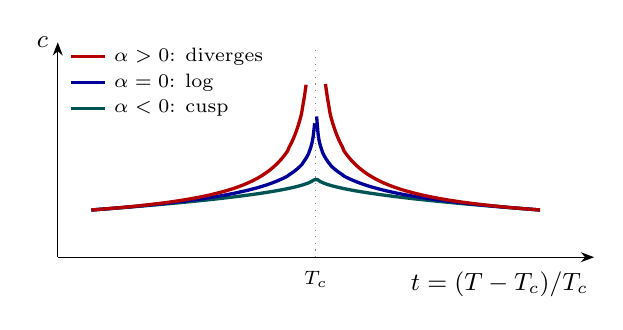
\begin{tikzpicture}[>=Stealth,font=\small,x=2.85cm,y=0.60cm]
  \draw[->] (-1.15,0) -- (1.24,0);
  \node[anchor=north east,inner sep=2pt] at (1.24,-0.18) {$t=(T-T_c)/T_c$};
  \draw[->] (-1.15,0) -- (-1.15,4.55) node[left]{$c$};
  \draw[dotted,gray] (0,0) -- (0,4.40);
  \draw[very thick,teal!65!black,samples=140,domain=-1:1,variable=\x,smooth]
       plot ({\x},{1+0.7*(1-sqrt(abs(\x)))});
  \draw[very thick,blue!60!black,samples=140,domain=0.0035:1,variable=\x,smooth]
       plot ({\x},{1-0.35*ln(abs(\x))});
  \draw[very thick,blue!60!black,samples=140,domain=-1:-0.0035,variable=\x,smooth]
       plot ({\x},{1-0.35*ln(abs(\x))});
  \draw[very thick,red!70!black,samples=140,domain=0.043:1,variable=\x,smooth]
       plot ({\x},{1+0.7*(pow(abs(\x),-0.5)-1)});
  \draw[very thick,red!70!black,samples=140,domain=-1:-0.043,variable=\x,smooth]
       plot ({\x},{1+0.7*(pow(abs(\x),-0.5)-1)});
  \node[anchor=north,font=\scriptsize] at (0,-0.10) {$T_c$};
  \draw[very thick,red!70!black]  (-1.09,4.25) -- (-0.94,4.25);
  \node[anchor=west,font=\scriptsize,inner sep=1.5pt] at (-0.92,4.25) {$\alpha>0$: diverges};
  \draw[very thick,blue!60!black] (-1.09,3.70) -- (-0.94,3.70);
  \node[anchor=west,font=\scriptsize,inner sep=1.5pt] at (-0.92,3.70) {$\alpha=0$: $\log$};
  \draw[very thick,teal!65!black] (-1.09,3.15) -- (-0.94,3.15);
  \node[anchor=west,font=\scriptsize,inner sep=1.5pt] at (-0.92,3.15) {$\alpha<0$: cusp};
\end{tikzpicture}
\caption{The three behaviours of
$c_{h}=(A_{\pm}/\alpha)\big(|t|^{-\alpha}-1\big)+B$, drawn with the same
amplitude and background for each. Only the \emph{sign} of $\alpha$ matters:
$\alpha>0$ gives a genuine divergence (red, here $\alpha=\tfrac12$, truncated at
the top of the frame), $\alpha=0$ the logarithm of the 2D Ising model (blue), and
$\alpha<0$ a finite peak approached with infinite slope --- a cusp (teal, here
$\alpha=-\tfrac12$). The exponents drawn are an order of magnitude larger than
the physical ones ($\alpha\simeq+0.110$ for 3D Ising, $\alpha\simeq-0.013$ for
3D XY), which is why the distinction, though sharp in principle, is so
demanding to establish in the laboratory.}
\label{fig:cusp}
\end{figure}

\begin{remark}[Where the non-analyticity comes from]
For any \emph{finite} system, $Z=\sum_i e^{-\beta E_i}$ is a finite sum of
positive exponentials, hence an entire function of $\beta$ with no zeros on the
real axis; $F=-k_BT\ln Z$ is therefore analytic and no phase transition can
occur. Non-analyticity is generated only in the thermodynamic limit, when the
complex zeros of $Z$ (Yang--Lee zeros in the fugacity plane, Fisher zeros in the
temperature plane) pinch the real axis. A phase transition is thus a property of
the limit, never of a finite sample --- which is precisely why finite-size
scaling is needed to extract critical behaviour from simulation
(Section~\ref{sec:fss}).
\end{remark}

\section{Heat and work}
\label{sec:heat}
\subsection{The clean derivation of \texorpdfstring{$\dbar Q_{\rm rev}=T\,dS$}{dQrev = T dS}}

The relation $\dbar Q_{\rm rev}=T\,dS$ is the hinge on which the rest of these
notes turn, so it is worth deriving in a way that uses nothing but the Gibbs state
itself. Take $\rho$ to be Gibbsian with $S=-k_B\sum_ip_i\ln p_i$, and let
$\lambda$ stand for whatever external parameters the experimenter controls
(volume, field, strain), work being by definition the energy delivered through
$\lambda$. Substituting
$\ln p_i = -\beta E_i-\ln Z$ gives the exact identity
\[
S=k_B\big(\ln Z+\beta U\big).
\]
Differentiate, using $d\ln Z=-U\,d\beta-\beta\,\dbar W$ (which follows from
$\ln Z$ depending on $\beta$ and on $\lambda$ through the $E_i$):
\[
\frac{dS}{k_B}=d\ln Z+U\,d\beta+\beta\,dU
=-U d\beta-\beta\dbar W+U d\beta+\beta\,dU
=\beta\big(dU-\dbar W\big),
\]
that is,
\[
\boxed{\;T\,dS=dU-\dbar W=\dbar Q_{\rm rev}\;}
\]
Three lines, and the only inputs are that the state is Gibbsian and that work is
the energy delivered through $\lambda$. The physical content is unchanged: heat is
energy transfer that is not accounted for by the controlled parameters, entropy
measures the spread of the distribution, and $T$ is the exchange rate between
them.

\subsection{Quasi-static is necessary but not sufficient}
\label{sec:clausius}

\subsubsection*{The Clausius inequality is a corollary of the second law}

The inequality used throughout this section is not an independent axiom, and it is
worth deriving it rather than quoting it, since everything below rests on it. The
only postulate needed is the second law in its entropy form:

\begin{quote}
\textbf{Second law.} For a thermally isolated composite system taken from one
equilibrium state to another, the total entropy does not decrease:
$\Delta S_{\rm tot}\geq0$, with equality if and only if the process is reversible.
\end{quote}

\paragraph{Why the integrated form is the primitive one.} The statement has been
written with $\Delta S_{\rm tot}$ rather than $dS_{\rm tot}$ deliberately, because
the differential version quietly presupposes more than it is entitled to. Entropy
is defined for \emph{equilibrium} states --- it is a function on the equilibrium
manifold of Section~\ref{sec:totaldiff} --- so writing $dS_{\rm tot}$ presumes
that the system possesses a well-defined entropy at every instant of the process.
For a violently irreversible process that is simply false: while a gas rushes into
a vacuum, or a shock traverses a sample, the system is in no equilibrium state and
there is no entropy there to differentiate.

What the second law needs, and all it needs, is that $S$ be defined at the
\emph{initial and final points}. Both are equilibrium states by hypothesis, so
$S_{\rm initial}$ and $S_{\rm final}$ exist; their difference is well defined
because $S$ is a state function; and $\Delta S_{\rm tot}\geq0$ is then a statement
about two numbers, committing to nothing whatever about the intervening history.
This is how Clausius and Planck state the law, and it is the form that survives
without further assumptions.

The differential form $dS_{\rm tot}\geq0$ is licensed in exactly two
circumstances, and it is worth knowing which is in force:
\begin{itemize}
\item \textbf{Quasi-static processes.} If the process is slow compared with all
internal relaxation times, then every intermediate state \emph{is} an equilibrium
state, the process traces a curve on the equilibrium manifold, and
$dS_{\rm tot}$ is a genuine one-form evaluated on that curve's tangent vector
(Section~\ref{sec:totaldiff}). Integrating it along the curve returns
$\Delta S_{\rm tot}$, so nothing is lost and nothing is assumed beyond
quasi-staticity. This is the case assumed in the derivation that follows, which is
why the Clausius inequality in differential form belongs to equilibrium
thermodynamics at all.
\item \textbf{Local equilibrium.} If the system is not globally equilibrated but
can be partitioned into cells each internally equilibrated on the timescale of
observation, one may define a local entropy density $s(\mathbf{r},t)$ and recover
not merely a differential but a \emph{local} statement,
\[
\frac{\partial s}{\partial t}+\nabla\!\cdot\mathbf{J}_s=\sigma\;\geq\;0 ,
\]
with $\mathbf{J}_s$ the entropy current and $\sigma$ the local production rate.
This is a genuine additional hypothesis, not a theorem; it is the foundation of
irreversible thermodynamics, and it fails exactly where one would expect --- in
shock fronts, in rarefied gases, and in glasses, whose slow coordinate is by
construction not equilibrated on any accessible timescale
(Section~\ref{sec:totaldiff}).
\end{itemize}
Absent either condition, ``$dS$'' should be read as shorthand for the integrated
statement applied to a chain of equilibrium states, and not as a claim that the
system had an entropy at every moment.

One asymmetry in the derivation below is worth noticing in this light. The
\emph{reservoir} is by construction always internally equilibrated --- that is
what makes it a reservoir --- so $S_{\rm res}$ is defined at every instant and
$dS_{\rm res}=-\dbar Q/T_{\rm res}$ carries no caveat at all. It is only the
\emph{system's} entropy that is subject to the endpoint restriction. So the
elimination of the reservoir can be carried out at the integrated level with no
quasi-static assumption whatever: $\Delta S_{\rm res}=-\int\dbar Q/T_{\rm res}$ is
exact, and $\Delta S_{\rm tot}=\Delta S+\Delta S_{\rm res}\geq0$ gives at once
\[
\boxed{\;\Delta S\;\geq\;\int\frac{\dbar Q}{T_{\rm res}}\;}
\]
between any two equilibrium states of the system, however violent the path
between them. This is the Clausius inequality in its primitive form, and the
differential version derived next is its quasi-static specialisation --- obtained
by the same two lines, read on a curve that lies in the equilibrium manifold. The
same distinction returns in the remark on $\Gamma_{\rm act}$ versus
$\Gamma_{\rm rev}$ later in this section: $\Delta S$ between two equilibrium states
is always defined, whereas an entropy \emph{along} an arbitrary process need not
be.

Now let the system of interest exchange heat $\dbar Q$ with a reservoir held at
temperature $T_{\rm res}$, take the process to be quasi-static for the system so
that $dS$ is meaningful, and take system $+$ reservoir together as the isolated
composite. The reservoir is by definition large enough to remain internally
equilibrated at $T_{\rm res}$ no matter what it gives up, so its own entropy
change is exact and computable:
\[
dS_{\rm res}=\frac{\dbar Q_{\rm res}}{T_{\rm res}}=-\frac{\dbar Q}{T_{\rm res}} ,
\]
the sign because the heat the system gains is the heat the reservoir loses.
Applying the second law to the composite,
\[
dS_{\rm tot}=dS+dS_{\rm res}=dS-\frac{\dbar Q}{T_{\rm res}}\;\geq\;0 ,
\]
which is the \emph{Clausius inequality}
\[
\boxed{\;dS \geq \frac{\dbar Q}{T_{\rm res}}\;}
\]
So Clausius' statement is the second law with the reservoir's entropy eliminated,
and nothing else. Note that the derivation locates the inequality precisely: it
compares the system's entropy change with the \emph{reservoir's} temperature, not
the system's --- which is why a finite temperature drop across the boundary
already costs entropy even when both bodies are internally equilibrated. The same
elimination, carried out for each choice of constraint, is what produces the
minimum principles of Section~\ref{sec:minimum}; Clausius' inequality and
``$F$ is minimised at fixed $T,V,N$'' are the same theorem stated for different
boundary conditions.

Since $dS_{\rm tot}$ is the total entropy \emph{produced}, it is convenient to
name it, $d\sigma\equiv dS_{\rm tot}\geq0$, and write the inequality as an
equality,
\[
dS = \frac{\dbar Q}{T_{\rm res}} + d\sigma ,
\]
so that $T\,dS = \dbar Q + T\,d\sigma \geq \dbar Q$ when $T=T_{\rm res}$, with
equality if and only if $d\sigma = 0$. The whole of the rest of this subsection is
a catalogue of ways to have $d\sigma>0$ while moving arbitrarily slowly.

It is a common error to treat ``quasi-static'' and ``reversible'' as synonyms.
They are not:

\begin{itemize}
\item \textbf{Quasi-static} means the process is slow compared with all internal
relaxation times, so the system passes through a continuous sequence of
equilibrium states. What this buys is that the path is a genuine \emph{curve on
the equilibrium manifold}, so that every state function --- $S$ included --- is
defined at each instant, and $\dbar Q$ and $\dbar W$ are one-forms evaluated on
the curve's tangent vector.

It is worth being explicit about why the intensive triple $(T,P,\mu)$ rather than
the extensive triple $(S,V,N)$ is the right thing to name here, since $(S,V,N)$
is the chart used everywhere else. The reason is that the three extensive
variables do not all test the same thing. $V$ and $N$ are \emph{mechanical and
counting} quantities: the volume of the container and the number of molecules
inside it are perfectly well defined during a shock wave or a turbulent stir, so
their availability says nothing about whether the system is in equilibrium. $S$,
by contrast, is defined only for equilibrium states, so quasi-staticity is
genuinely required for it --- and quasi-staticity is exactly what supplies it.
$T$, $P$, and $\mu$ are then singled out for two further reasons. First, they are
\emph{derivatives} of the fundamental relation, so they exist only where the
system actually sits on the equilibrium manifold, making them the sharpest
diagnostic of quasi-staticity: a fluid with a temperature gradient across it has a
$V$ and an $N$ but no single $T$. Second, they are what actually appears in the
one-forms $\dbar Q_{\rm rev}=T\,dS$ and $\dbar W=-P\,dV+\mu\,dN$, so it is their
existence, and their equality with the reservoir's values, that the argument
needs. Put compactly: quasi-staticity gives $S$, and hence the whole chart
$(S,V,N)$, its meaning; and it is then the derivatives $T$, $P$, $\mu$ whose
well-definedness the heat and work forms consume.
\item \textbf{Reversible} means quasi-static \emph{and} dissipationless: no
friction, no finite temperature or pressure drops across the boundary, no
hysteresis, no chemical reaction running downhill.
\end{itemize}

Quasi-staticity is necessary for $\dbar Q = T\,dS$ but not sufficient. Standard
counterexamples, all arbitrarily slow yet all with $\dbar Q < T\,dS$:
\begin{itemize}
\item \textbf{Joule (paddle-wheel) heating.} Stir a thermally isolated fluid
infinitesimally slowly. The fluid remains in equilibrium throughout, so it is
quasi-static; $\dbar Q = 0$ because the vessel is adiabatic; yet $dS > 0$ since
the work is degraded into internal energy. Here $T\,dS = T\,d\sigma$ entirely.
\item \textbf{Compression against sliding friction.} The gas is in equilibrium at
every instant, but the frictional work heats the system.
\item \textbf{Heat flow across a finite $\Delta T$.} If the reservoir is at
$T_{\rm res} \neq T$, then $\dbar Q/T_{\rm res} < \dbar Q/T = dS$ for heating.
The system alone is quasi-static; the composite is not.
\item \textbf{Hysteretic condensed-matter systems.} Domain-wall depinning
(Barkhausen noise), martensitic transformations, and vortex-lattice motion all
dissipate a finite amount of work per cycle no matter how slowly the field is
swept. The $\omega \to 0$ limit of the hysteresis loop area is nonzero, so the
quasi-static limit is genuinely irreversible.
\item \textbf{Glasses and slow degrees of freedom.} If some internal variable has
a relaxation time comparable to the measurement, the system is never truly
equilibrated. This is why the specific heat of a glass former is
frequency-dependent, $c(\omega) = c'(\omega) - i c''(\omega)$, with $c''$
measuring precisely the dissipation that spoils $\dbar Q = T\,dS$.
\end{itemize}

\begin{remark}[Are glasses outside statistical mechanics?]
No --- but which parts of the apparatus survive is worth separating, since the
last bullet can leave the impression that glasses are simply off-limits.

\emph{Statistical mechanics survives untouched.} A glass is an ordinary
Hamiltonian system: the microstates, the phase-space measure, and the Boltzmann
weight are all exactly what they always were. What is lost is not the framework
but \emph{ergodicity on the experimental timescale}: the trajectory explores only
one basin of the energy landscape instead of the whole of it, so time averages
stop equalling full ensemble averages. The standard repair is to average over the
restricted region actually visited --- a \emph{restricted} or constrained
ensemble --- which is the same device used for a ferromagnet below $T_c$ (where
one does not average over both magnetisation directions) and for any
symmetry-broken phase. Nothing about that is special to glasses; the difference is
only that the restriction is imposed by kinetics rather than by symmetry.

\emph{Equilibrium thermodynamics survives in the constrained sense.} Below $T_g$
the glass is in constrained equilibrium at a frozen configurational coordinate,
which is exactly the second regime of Section~\ref{sec:totaldiff}. All the state
functions exist as functions of $(S,V,N;\xi)$, and the practical bookkeeping
device is the \emph{fictive temperature} $T_f$: the temperature at which the
frozen structure would be the equilibrium one. Measured properties then depend on
$T$ through the fast degrees of freedom and on $T_f$ through the frozen ones. The
residual entropy at $T\to0$ --- the configurational entropy of the basin
multiplicity --- is a genuine, measurable quantity, obtained by comparing the
calorimetric entropy of the glass with that of the crystal, and it is not a
violation of the third law but a statement that the constrained system has more
than one accessible ground state.

\emph{What genuinely fails.} Three things. (i) The identification $\dbar
Q=T\,dS$, whenever the measurement timescale is comparable to $\tau_\xi$; this is
the content of the last bullet, and it is why $c(\omega)$ is complex. (ii) The
fluctuation--dissipation theorem in its equilibrium form: response and correlation
are no longer related by a single temperature, and the deviation is
parametrised by an effective temperature $T_{\rm eff}(\omega)>T$ that
characterises the slow modes. (iii) Uniqueness of the state: properties depend on
preparation history (cooling rate, ageing time), so there is no function of
$(T,P)$ alone to tabulate.

\emph{And what replaces them.} A large body of theory does exactly this. The
Adam--Gibbs and random first-order transition pictures relate the relaxation time
to a configurational entropy computed by equilibrium statistical mechanics; the
replica and cavity methods compute that entropy for mean-field models exactly;
mode-coupling theory derives $\tau_\xi(T)$ from equilibrium static correlators
alone; the Edwards ensemble assigns a flat measure over jammed configurations at
fixed volume, with a ``compactivity'' playing the role of temperature; and
stochastic thermodynamics gives exact fluctuation theorems that hold arbitrarily
far from equilibrium and reduce to the Clausius inequality above on averaging. So
the correct statement is not that glasses escape statistical mechanics, but that
they require the non-ergodic and non-equilibrium parts of it.
\end{remark}

\begin{remark}[Two different paths, not one path described two ways]
A frequent and entirely reasonable objection to the standard recipe ``compute
$\Delta S$ along a reversible path'' is that it sounds self-contradictory: a path
built out of reversible steps \emph{is} reversible, so how can the process have
been violently irreversible?

The answer is that two \emph{different} paths are in play, and only their
endpoints are shared. Call them
\begin{align*}
\Gamma_{\rm act}&:\ \text{what the system actually did},\\
\Gamma_{\rm rev}&:\ \text{an auxiliary reversible curve with the same endpoints.}
\end{align*}
$\Gamma_{\rm rev}$ is not a re-description of $\Gamma_{\rm act}$ and is not
claimed to be physically realised during the experiment; it is a curve on the
equilibrium manifold chosen for the convenience of doing an integral. Indeed
$\Gamma_{\rm act}$ is typically not a curve on that manifold at all --- during a
free expansion the gas is not in any equilibrium state, so it has no location in
the state space to trace out. What the two share is only the initial and final
equilibrium points, and since $S$ is a state function that is all $\Delta S$
depends on:
\[
\Delta S=\int_{\Gamma_{\rm rev}}dS=\int_{\Gamma_{\rm act}}dS=S_2-S_1 ,
\]
the middle equality being exactness of $dS$, not any claim that the two processes
resemble each other. By contrast $\dbar Q$ is \emph{not} exact, so
$\int_{\Gamma_{\rm rev}}\dbar Q\neq\int_{\Gamma_{\rm act}}\dbar Q$ in general, and
substituting one for the other is exactly the error the caveat warns against.

The classic example makes the two paths concrete. An ideal gas doubles its volume:
\begin{itemize}
\item $\Gamma_{\rm act}$ --- \emph{free expansion.} The partition is removed and
the gas rushes into vacuum with the vessel isolated. Then $Q=0$ and $W=0$, hence
$\Delta U=0$, hence (for an ideal gas) $T_2=T_1$. Wildly irreversible; no
intermediate equilibrium states exist.
\item $\Gamma_{\rm rev}$ --- \emph{isothermal quasi-static expansion.} The same
gas, in contact with a bath at $T_1$, pushes a piston out infinitely slowly to the
same final volume. Here $W=-Nk_BT\ln2\neq0$ and $Q=+Nk_BT\ln2\neq0$.
\end{itemize}
The two processes exchange completely different amounts of heat and work --- one
exchanges none of either --- yet both run from $(T_1,V)$ to $(T_1,2V)$, so both
have
\[
\Delta S=Nk_B\ln 2 .
\]
For $\Gamma_{\rm rev}$ this equals $Q/T_1$; for $\Gamma_{\rm act}$ it does not,
since $Q=0$ there and the entire $\Delta S$ is entropy production. So the
restriction to reversible processes applies to identifying $T\,dS$ with the
\emph{heat actually exchanged}, never to the value of $\Delta S$. Nothing has been
claimed to be simultaneously reversible and irreversible.
\end{remark}

\begin{remark}[Why $c_V$ is unusually robust]
At fixed volume and particle number no work is done, so $\dbar Q = dU$ \emph{regardless
of reversibility}. Hence $C_V = (\partial U/\partial T)_{V,N}$ holds even for
irreversible heating, which is why constant-volume calorimetry is well behaved.
The step $\dbar Q = T\,dS$ is needed only to re-express this as $C_V = T(\partial
S/\partial T)_{V,N}$ and thereby connect it to the free energy. For $C_P$, or for
any process involving mechanical work, the reversibility caveat bites in earnest.
\end{remark}

\section{Exact and inexact differentials}
\label{sec:exact}

A state function has an exact differential,
\[
df=
\left(\frac{\partial f}{\partial x}\right)_y dx+
\left(\frac{\partial f}{\partial y}\right)_x dy,
\]
so that $\int_1^2 df=f_2-f_1$ and $\oint df=0$: the integral depends only on
endpoints. Heat and work are transfer processes, not properties of a state, and
their differentials are inexact:
\[
\oint\dbar Q\neq 0,\qquad \oint\dbar W\neq 0 .
\]
Indeed a heat engine is precisely a device exploiting $\oint \dbar Q \neq 0$.

For a general one-form $\omega = A(x,y)\,dx + B(x,y)\,dy$, exactness on a simply
connected domain requires
\[
\boxed{\;\frac{\partial A}{\partial y}=\frac{\partial B}{\partial x}\;}
\]
Applied to $dU$, $dF$, $dG$, $d\Omega$, this condition generates the Maxwell
relations; from $dF = -S\,dT - P\,dV$ and $dG = -S\,dT + V\,dP$,
\[
\left(\frac{\partial S}{\partial V}\right)_{T,N}
=\left(\frac{\partial P}{\partial T}\right)_{V,N},
\qquad
\left(\frac{\partial S}{\partial P}\right)_{T,N}
=-\left(\frac{\partial V}{\partial T}\right)_{P,N}.
\]
These are the workhorses that convert an unmeasurable entropy derivative into a
measurable equation-of-state derivative.

Although $\dbar Q_{\rm rev}$ is inexact, dividing by $T$ makes it exact:
\[
\boxed{\;\frac{\dbar Q_{\rm rev}}{T}=dS\;}
\]
so $1/T$ is an \emph{integrating factor}. That such a factor exists at all is the
content of Carath\'eodory's formulation of the second law: in any neighbourhood of
any equilibrium state there are states unreachable by adiabatic processes, which
forces $\dbar Q_{\rm rev}$ to admit an integrating factor, and the universality of
$T$ follows from consistency between coupled systems.

\section{Thermodynamic potentials}
\label{sec:potentials}

\subsection{What a Legendre transform does, and why one is needed}
\label{sec:legendre}

\subsubsection*{The problem: changing variables without losing information}

We want to describe the system using an \emph{intensive} control variable,
because that is what an experiment fixes: a sample sits in a bath at temperature
$T$, not at prescribed entropy. The obvious move is naive substitution: compute
$T=(\partial U/\partial S)_{V,N}$, invert to get $S(T,V,N)$, and define
\[
\tilde U(T,V,N)\equiv U\big(S(T,V,N),V,N\big).
\]

\paragraph{A red herring first: invertibility.} One might expect the trouble to
sit in the inversion step, on the grounds that $T(S)$ is in general a nonlinear
function. It does not, and the distinction is worth drawing because it isolates
where the real problem is. Nonlinearity is not the issue: what a function needs
in order to be invertible is \emph{strict monotonicity}, not linearity, and
$S\mapsto T$ has it wherever the system is thermally stable, since
\[
\left(\frac{\partial T}{\partial S}\right)_{V,N}
=\left(\frac{\partial^{2}U}{\partial S^{2}}\right)_{V,N}=\frac{T}{C_V}>0
\qquad\text{whenever } C_V>0 ,
\]
and Section~\ref{sec:whyconvex} shows that $C_V>0$ --- equivalently, strict
convexity of $U$ in $S$ --- is not an assumption but a consequence of the second
law. So $T(S)$ is strictly increasing and the inverse function theorem supplies a
smooth $S(T,V,N)$ on the whole stable branch, however nonlinear the relation:
$T=\alpha S^{3}+\beta e^{S}$ with $\alpha,\beta>0$ is thoroughly nonlinear and
thoroughly invertible.

Invertibility \emph{does} fail, but for a sharper reason than nonlinearity ---
loss of \emph{strict} convexity. Two cases, both already encountered:
\begin{itemize}
\item At a first-order transition $U$ is affine in $S$ along a tie line
(Figure~\ref{fig:firstorder}b), so $C_V=\infty$ and $(\partial T/\partial
S)_{V,N}=0$ there. An entire interval of $S$ maps to the single value $T_t$, and
$S(T)$ simply does not exist as a function. This is the genuine breakdown, and the
Legendre--Fenchel transform of Section~\ref{sec:maxwell} is what repairs it.
\item Inside a spinodal region a \emph{computed} mean-field $U$ can be concave,
$C_V<0$, making $T(S)$ non-monotonic and $S(T)$ multivalued. As
Section~\ref{sec:maxwell} argues, the exact $U$ is never concave and such states
are not physical.
\end{itemize}
Set both aside for the moment. On the stable branch the inversion is entirely
sound --- and the naive substitution is a disaster anyway. That is the point of
this subsection.

\paragraph{The toy example, and why it does not by itself settle the matter.} The
usual illustration is
\[
U(S)=\tfrac12(S+a)^{2},
\]
with $a$ a material constant. Then $T=\partial U/\partial S=S+a$, so $S=T-a$ and
\[
\tilde U(T)=\tfrac12 T^{2},
\]
in which $a$ has vanished, whereas the Legendre transform
\[
F(T)=\big(U-TS\big)\big|_{S=T-a}=-\tfrac12T^{2}+aT
\]
retains it, and $S=-\partial F/\partial T=T-a$ recovers the original relation
exactly.

Suggestive --- but taken alone this does not prove what it is usually asked to
prove, and the objection is a fair one. If the physical domain of $S$ is known,
say $S\geq0$, then $T=S+a$ has range $T\geq a$, so $a$ is recoverable from the
\emph{domain} of $\tilde U$ even though it is absent from its \emph{values}. Here
physics would even supply that datum for free: the third law forces $S\to0$ as
$T\to0$, which in this model means $a=0$. On a one-variable example, then, the
information is not destroyed but merely relocated from the function's values to
its domain, and the conclusion ``$\tilde U(T)$ cannot possibly determine $U(S)$''
is not yet established.

\paragraph{It is established as soon as there is a second variable.} Real
fundamental relations are $U(S,V,N)$, and there the loss is not a number but a
whole function --- which no statement about domains can restore. The cleanest
illustration is the classical monatomic ideal gas, whose energy is
volume-independent:
\[
U=\tfrac32Nk_BT
\qquad\Longrightarrow\qquad
\tilde U(T,V,N)=\tfrac32 Nk_BT .
\]
Consider what this $\tilde U$ knows about the gas: nothing at all about $V$. It
cannot produce the equation of state, since $-(\partial\tilde U/\partial V)$ is
identically zero rather than $Nk_BT/V$; it cannot distinguish an ideal gas from
any other substance whose energy happens not to depend on volume; and no
restriction of its domain can repair the deficit, because the missing object is a
function of $V$ and not a constant. The Helmholtz free energy, by contrast,
\[
F(T,V,N)=-Nk_BT\left[\ln\frac{V}{N\lambda_T^{3}}+1\right],
\]
returns $P=-(\partial F/\partial V)_{T,N}=Nk_BT/V$ and
$S=-(\partial F/\partial T)_{V,N}$, the Sackur--Tetrode entropy, at once. Naive
substitution has erased the mechanical equation of state entirely; the Legendre
transform has kept it.

\paragraph{Exactly what is lost: the first-order differential equation.} The
general statement can be made precise, and doing so is what justifies the claim
that recovering $U$ from $\tilde U$ requires solving a differential equation.

Since $\tilde U=U$ evaluated at $S=S(T,V,N)$, and $F=U-TS$ with
$S=-(\partial F/\partial T)_{V,N}$, the two objects are related by
\[
\boxed{\;\tilde U=F-T\left(\frac{\partial F}{\partial T}\right)_{V,N}\;}
\]
Getting $\tilde U$ from $F$ is therefore a \emph{differentiation}. Going the other
way means reading the boxed relation as an equation to be solved for $F$ with
$\tilde U$ given, and at each fixed $(V,N)$ it is a linear first-order ODE in $T$,
\[
\frac{\partial F}{\partial T}-\frac{F}{T}=-\frac{\tilde U}{T} .
\]
Its homogeneous version $\partial F/\partial T=F/T$ has general solution
$F_{\rm hom}=C\,T$, where $C$ is constant in $T$ but may be an arbitrary function
of the other variables. So the general solution is
\[
F(T,V,N)=F_{\rm part}(T,V,N)+C(V,N)\,T ,
\]
and $\tilde U$ fixes $F$ --- equivalently $U$ --- only up to that arbitrary
$C(V,N)$. This is the differential equation in question, and $C(V,N)$ is precisely
the ``constant of integration'' that carries the lost information. In one variable
$C$ degenerates to a single number, which is why the toy example above could be
rescued by a domain argument; in the physical case it is an entire function of
$(V,N)$, and nothing outside $\tilde U$ can supply it.

What does the ambiguity mean physically? Adding $C(V,N)\,T$ to $F$ shifts
$S=-(\partial F/\partial T)_{V,N}$ by the constant $-C(V,N)$ at each $(V,N)$ and
leaves $U=F+TS$, viewed as a function of $(T,V,N)$, unchanged --- which is exactly
why $\tilde U$ cannot see it. In the energy representation the same ambiguity
reads
\[
U_C(S,V,N)\;\equiv\;U\big(S+C(V,N),\,V,\,N\big),
\]
and one verifies immediately that every member of this family has the same
$\tilde U$: the temperature is $T=(\partial U_C/\partial S)_{V,N}=U_S(S+C,V,N)$,
so the substitution $\sigma=S+C(V,N)$ carries the problem back to the original one.
These are not relabellings of one substance. Their pressures differ:
\[
-P_C=\left(\frac{\partial U_C}{\partial V}\right)_{S,N}
=T\,\frac{\partial C}{\partial V}-P
\qquad\Longrightarrow\qquad
P_C=P-T\,\frac{\partial C}{\partial V} .
\]
Applied to the ideal gas with $C(V,N)=+Nk_B\ln(V/V_0)$, this gives $P_C\equiv0$: a
formally admissible fundamental relation,
$U_C(S,N)=c\,N^{5/3}V_0^{-2/3}e^{2S/3Nk_B}$, describing a substance with no
mechanical equation of state whatever, and with $\tilde U_C=\tfrac32Nk_BT$
identical to the gas's. Two materials as different as that share the same
$\tilde U$; they do not share the same $F$.

\paragraph{The asymmetry that matters.} Recovering $U$ from the Legendre transform
$F$, by contrast, requires no integration at all: $S=-(\partial F/\partial
T)_{V,N}$ is a differentiation, and $U=F+TS$ then follows algebraically, with only
an inversion $S\leftrightarrow T$ --- guaranteed, as above, by $C_V>0$ --- needed
to express the result in the variables $(S,V,N)$. Differentiating introduces no
constants of integration; integrating does. That asymmetry, and not any subtlety
about invertibility, is why $F$ is a potential and $\tilde U$ is merely a
function.

\subsubsection*{The geometric reason it works}

The Legendre transform works because a convex function can be described in two
equivalent ways: as the set of points $\big(S,U(S)\big)$, or as the envelope of
its family of tangent lines. The tangent at $S_0$ has slope $T=U'(S_0)$ and
satisfies
\[
y=U(S_0)+T(S-S_0)=T\,S+\underbrace{\big[U(S_0)-TS_0\big]}_{=\,F(T)} ,
\]
so $F(T)$ is exactly the \emph{intercept} of the tangent line of slope $T$.
Specifying all (slope, intercept) pairs specifies the envelope, hence $U(S)$: no
information is lost. Naive substitution keeps only the slopes and discards the
intercepts, which is the toy example above.

\subsubsection*{Why $U$ is convex in $S$}
\label{sec:whyconvex}

Invertibility of $S\mapsto T$ requires $U$ to be strictly convex in $S$, and this
is not an assumption --- it follows from the second law applied to a composite
system.

Take a system in equilibrium and imagine dividing it conceptually into two equal
halves that may exchange energy. At fixed total energy $2E$, the second law says
total entropy is maximal at the actual equilibrium, which by symmetry is equal
division. So for any $E_1,E_2$ with $E_1+E_2=2E$,
\[
S(E_1)+S(E_2)\;\leq\;2\,S\!\left(\frac{E_1+E_2}{2}\right).
\]
This is midpoint concavity; with continuity it gives concavity of $S(E)$ outright.
Since also $\partial S/\partial E = 1/T>0$, $S$ is concave \emph{and increasing},
and the inverse function of a concave increasing function is convex increasing.
Hence $U(S)$ is convex. Equivalently, in differential form,
\[
\left(\frac{\partial^{2}U}{\partial S^{2}}\right)_{V,N}
=\left(\frac{\partial T}{\partial S}\right)_{V,N}=\frac{T}{C_V}\;\geq\;0
\quad\Longleftrightarrow\quad C_V\geq0,
\]
which is thermal stability. Convexity of $U$ in $S$, positivity of $C_V$, and
entropy maximisation of the composite are three statements of one fact. Where
stability fails --- inside a spinodal region --- convexity fails too, the map
$S\mapsto T$ is no longer invertible, and the Legendre transform needs the
repair described in Section~\ref{sec:maxwell}.

\subsubsection*{Is the Legendre transform a minimisation?}

Strictly, no, and the loose claim that ``the Legendre transform \emph{is} a
minimisation'' should be stated more carefully. The classical Legendre transform
is defined by a stationarity condition and a substitution:
\[
F(T)=U(S^\ast)-TS^\ast, \qquad S^\ast \text{ solving } \frac{\partial
U}{\partial S}=T .
\]
There is no minimisation in that definition. What is true is that for a convex
differentiable $U$ this coincides with the \emph{Legendre--Fenchel}
transform,\footnote{\label{fn:inf}\textbf{$\inf$ and $\sup$.} For a set of real
numbers $A$, the \emph{infimum} $\inf A$ is its greatest lower bound: the largest
number that is $\leq$ every element of $A$. The notation $\inf_{S}g(S)$ means
$\inf\{g(S):S\ \text{admissible}\}$, the greatest lower bound of the values $g$
takes as $S$ ranges over its domain. The point of writing $\inf$ rather than
$\min$ is that the infimum always exists (in $\mathbb{R}\cup\{-\infty\}$) whereas
a minimum need not be attained: $g(S)=e^{-S}$ on $[0,\infty)$ has $\inf g=0$ but
no minimum, and $g(S)=S$ on the open interval $(0,1)$ has $\inf g=0$, again
attained at no admissible $S$. When the infimum \emph{is} attained --- which for a
strictly convex $g$ tending to $+\infty$ at the ends of its domain it always is
--- then $\inf$ and $\min$ coincide, and that is the situation throughout this
section: the stationarity condition $\partial U/\partial S=T$ locates the
minimiser $S^{\ast}$ and $F(T)=U(S^{\ast})-TS^{\ast}$. The value $-\infty$ is not
idle bookkeeping either: $\inf_S[U(S)-TS]=-\infty$ is precisely how the
variational form reports that $T$ lies outside the range of $\partial U/\partial
S$, i.e.\ that no state of the system has that temperature. The mirror notion
$\sup$ is the least upper bound.}
\[
\boxed{\;F(T)=\inf_{S}\big[\,U(S)-TS\,\big]\;}
\]
because for convex $U$ the function $S\mapsto U(S)-TS$ is convex and its unique
stationary point is its global minimum. So the two constructions agree on the
domain where the classical transform is defined, and it is the variational form
that is more general: it is well defined for non-differentiable and even
non-convex $U$, and applying it twice returns not $U$ but its convex hull,
\[
U^{\ast\ast}=\operatorname{conv}U .
\]
That last property is not a technicality --- it is the Maxwell construction, as
Section~\ref{sec:maxwell} shows.

The variational form is also the bridge to thermodynamics, and this is why it is
worth having. In $\inf_S[U(S)-TS]$ the variable $S$ plays the role of an
\emph{unconstrained internal variable}: a system coupled to a bath is free to
exchange energy and thereby to choose its entropy, and it settles at the value
minimising $U-TS$. The stationarity condition $\partial U/\partial S=T$ is then
the statement that system and bath have reached a common temperature. The
minimum principle of Section~\ref{sec:minimum} and the Legendre--Fenchel form of
the transform are therefore the same equation read in two directions --- but they
are not the same as the bare definition of the transform, and conflating all
three obscures where the physics enters.

\subsection{The family}

\paragraph{Internal energy.} Natural variables $(S,V,N)$:
\[
\boxed{\;dU=T\,dS-P\,dV+\mu\,dN\;}
\]

\paragraph{Enthalpy.}
\[
\boxed{\;H=U+PV\;},\qquad
\boxed{\;dH=T\,dS+V\,dP+\mu\,dN\;}
\]
so $H=H(S,P,N)$. At constant $P$ and $N$, $dH = \dbar Q_{\rm rev}$, which is why
enthalpy is the natural bookkeeping variable for calorimetry at atmospheric
pressure and gives $C_P = (\partial H/\partial T)_{P,N}$.

\paragraph{Helmholtz free energy.}
\[
\boxed{\;F=U-TS\;},\qquad
\boxed{\;dF=-S\,dT-P\,dV+\mu\,dN\;}
\]
so $F=F(T,V,N)$, and
\[
S=-\left(\frac{\partial F}{\partial T}\right)_{V,N},\quad
P=-\left(\frac{\partial F}{\partial V}\right)_{T,N},\quad
\mu=\left(\frac{\partial F}{\partial N}\right)_{T,V}.
\]

\paragraph{Gibbs free energy.}
\[
\boxed{\;G=U-TS+PV=F+PV\;},\qquad
\boxed{\;dG=-S\,dT+V\,dP+\mu\,dN\;}
\]
so $G=G(T,P,N)$, with $S = -(\partial G/\partial T)_{P,N}$ and $V = (\partial
G/\partial P)_{T,N}$. Since $G=\mu N$, the chemical potential is the Gibbs free
energy per particle.

\paragraph{Grand potential.}
\[
\boxed{\;\Omega=U-TS-\mu N=F-\mu N\;},\qquad
\boxed{\;d\Omega=-S\,dT-P\,dV-N\,d\mu\;}
\]
so $\Omega=\Omega(T,V,\mu)$, and
\[
S=-\left(\frac{\partial\Omega}{\partial T}\right)_{V,\mu},\quad
P=-\left(\frac{\partial\Omega}{\partial V}\right)_{T,\mu},\quad
N=-\left(\frac{\partial\Omega}{\partial\mu}\right)_{T,V}.
\]
The grand potential is indispensable for \emph{both} quantum statistics, and for
essentially the same technical reason in each case: only in the grand ensemble
does the many-body problem factorise mode by mode,
$\Xi=\prod_{k}\xi_{k}$, because the constraint $\sum_kn_k=N$ that couples the
modes has been traded for a Lagrange multiplier $\mu$. The Fermi--Dirac and
Bose--Einstein distributions both emerge from this factorisation and are
essentially intractable at fixed $N$. Concretely:
\begin{itemize}
\item \emph{Fermions}: electrons in a metal exchanging with leads, a gate that
holds $\mu$, semiconductor doping, and any Landauer-type transport problem where
two reservoirs impose $\mu_L\neq\mu_R$.
\item \emph{Bosons}: Bose--Einstein condensation, where the condensate is defined
precisely by $\mu\to\varepsilon_0$ and the saturation of the excited-state
population is a grand-canonical statement; the Mott lobes of the Bose--Hubbard
model, which are drawn in the $(\mu,t)$ plane and whose flat-topped structure at
integer filling exists only because $\mu$ is the control variable; superfluid
${}^4$He; and cold-atom clouds in a trap, where the local density approximation
treats each region as grand-canonical with $\mu_{\rm loc}=\mu-V_{\rm trap}(r)$.
\item \emph{Bosons with non-conserved number}: photons and phonons have no
conservation law at all, so $\mu=0$ identically and the grand and canonical
descriptions coincide --- black-body radiation and the Debye model are
grand-canonical calculations in disguise.
\end{itemize}

\subsection{The minimum principle}
\label{sec:minimum}

\emph{Should the potential be minimised? Yes --- provided one is careful about
which potential, with respect to what, and holding what fixed.} The precise
statement is:

\begin{quote}
\textbf{At fixed values of its natural variables, the appropriate thermodynamic
potential is minimised with respect to all remaining unconstrained internal
degrees of freedom.}
\end{quote}

Every clause matters. ``At fixed natural variables'' identifies which potential
applies. ``With respect to internal degrees of freedom'' identifies what is being
varied --- and that phrase is ambiguous enough to be worth pinning down, because
the term is used for at least three different things in the literature and only
one of them is meant here. There are three levels of description in play:

\begin{enumerate}
\item \textbf{Microscopic degrees of freedom}: the atomic positions and momenta
$\{\mathbf{r}_i,\mathbf{p}_i\}$, or the quantum many-body state. These are
\emph{not} what is minimised over. They are \emph{summed} over --- traced out by
the partition function --- and the minimum principle sits at a level of
description from which they have already disappeared. Minimising the energy over
atomic coordinates at $T=0$ is a different (and also useful) statement; it is not
this one.
\item \textbf{The natural variables} of the potential: $(T,V,N)$ for $F$,
$(T,P,N)$ for $G$, and so on. These are \emph{not} varied either --- they are
precisely what is held fixed, by the walls and the reservoirs. Minimising $F$
``over $T$'' is meaningless.
\item \textbf{Macroscopic internal variables}: the remaining coarse-grained,
collective quantities that the constraints leave undetermined. \emph{These} are
what one minimises over.
\end{enumerate}

The third category is exactly the set of $\xi$-type variables introduced in
Section~\ref{sec:totaldiff}: macroscopic averages over many microscopic degrees of
freedom, sharply defined and non-fluctuating in the thermodynamic limit, but not
pinned down by the imposed constraints. Typical members:
\begin{itemize}
\item the partitioning of a conserved quantity between subsystems --- the energies
$E_1,E_2$ of two halves at fixed $E_1+E_2$, or the particle numbers $N_1,N_2$ at
fixed $N_1+N_2$;
\item the extent of a chemical reaction, $\xi$, at fixed total elemental
composition;
\item the volume fraction $x$ of a coexisting phase at fixed total volume;
\item an order parameter --- magnetisation, superconducting gap, staggered moment,
strain, nematic director;
\item the position of an internal partition, or an internal pressure or
temperature difference, in a compound system.
\end{itemize}
The test for membership is operational: a variable belongs on this list if the
system can change it \emph{without} violating any imposed constraint. Once it can,
the second law says the composite will change it in whichever direction lowers the
relevant potential, and equilibrium is where no such direction remains.

\paragraph{Derivation.} The only fundamental extremum principle is the second law:
for an \emph{isolated} composite, $S_{\rm tot}$ is maximised. Everything else
follows by eliminating the reservoir. Let the system exchange heat with a
reservoir at temperature $T$. The reservoir is large, so it stays in equilibrium
and $dS_{\rm res} = -\dbar Q/T$. Then
\[
dS_{\rm tot}=dS_{\rm sys}+dS_{\rm res}=dS-\frac{\dbar Q}{T}\geq 0
\quad\Longrightarrow\quad \dbar Q \leq T\,dS .
\]
Now insert the first law $\dbar Q = dU - \dbar W$ for the various constraints:

\begin{center}
\begin{tabular}{lll}
\toprule
Held fixed & Second law becomes & Equilibrium condition\\
\midrule
$E,V,N$ (isolated) & $dS \geq 0$ & $S$ \emph{maximum}\\
$S,V,N$ & $dU \leq 0$ & $U$ minimum\\
$S,P,N$ & $dH \leq 0$ & $H$ minimum\\
$T,V,N$ & $dF \leq 0$ & $F$ minimum\\
$T,P,N$ & $dG \leq 0$ & $G$ minimum\\
$T,V,\mu$ & $d\Omega \leq 0$ & $\Omega$ minimum\\
\bottomrule
\end{tabular}
\end{center}

For the $T,V,N$ case explicitly: at fixed $V$ no work is done, so $\dbar W = 0$
and $\dbar Q = dU$; the inequality $dU \leq T\,dS$ at fixed $T$ is
$d(U - TS) = dF \leq 0$. The potential can only decrease, so it decreases until
it cannot: it is a Lyapunov function whose minimum is equilibrium. The sign flip
relative to entropy maximisation comes entirely from the reservoir's entropy
appearing with the opposite sign.

\paragraph{The statistical-mechanical version.} There is an exact variational
statement underneath. Define, for an arbitrary trial density matrix $\rho$,
\[
\mathcal{F}[\rho]=\Tr(\rho\hat H)+k_BT\,\Tr(\rho\ln\rho).
\]
Then $\mathcal{F}[\rho]-F=k_BT\,D(\rho\|\rho_{\rm eq})\geq0$, with equality only
for $\rho=\rho_{\rm eq}$. So the equilibrium density matrix is the \emph{global}
minimiser of $\mathcal{F}$, and $F=-k_BT\ln Z$ is the minimum value. This is the
Gibbs variational principle; the Gibbs--Bogoliubov inequality $F\leq
F_0+\langle\hat H-\hat H_0\rangle_0$, the workhorse of variational mean-field
theory, is the same statement with a restricted trial family.

\paragraph{The condensed-matter version.} In practice one introduces an order
parameter $\phi$ --- magnetisation, superconducting gap, staggered moment, strain
--- and builds a \emph{constrained} free energy $F(T,V,N;\phi)$. It is worth
defining this object properly, because the shorthand ``$\phi$ is held fixed by an
artificial conjugate field'' is at best misleading: a field fixes only the
\emph{mean} of $\phi$, and the construction it produces is not always the one
Landau theory needs.

The honest definition is a \emph{partial} trace. Let $\hat\phi$ be the operator
(or, classically, the phase-space function) whose value is the order parameter,
for instance $\hat\phi=M^{-1}\sum_i\hat\sigma^z_i$ for magnetisation per site.
Then
\[
\boxed{\;e^{-\beta F(T,V,N;\phi)}\;=\;\Tr\Big[\,\delta\big(\hat\phi-\phi\big)\,
e^{-\beta\hat H}\Big]\;}
\]
i.e.\ one sums the Boltzmann weight over only those microstates whose order
parameter has the prescribed value $\phi$, instead of over all of them. Nothing
artificial is added; the constraint is a restriction of the sum. Equivalently
$F(\phi)=-k_BT\ln P(\phi)+\text{const}$, where $P(\phi)$ is the probability
distribution of the order parameter in the ordinary canonical ensemble --- so
$F(\phi)$ is a measurable object, and in a simulation it is exactly what a
histogram of $\phi$ reports. Summing over $\phi$ recovers the unconstrained free
energy, and in the thermodynamic limit that sum is dominated by its smallest
term:
\[
e^{-\beta F_{\rm eq}}=\int\! d\phi\; e^{-\beta F(\phi)}
\quad\Longrightarrow\quad
F_{\rm eq}(T,V,N)=\min_{\phi}F(T,V,N;\phi)+O(\ln V),
\qquad
\left.\frac{\partial F}{\partial \phi}\right|_{\phi_{\rm eq}}=0 .
\]

The conjugate-field route is a \emph{different} construction that agrees with this
one only conditionally, and the difference is instructive. Adding a source $h$
coupled to $\hat\phi$ gives an ordinary, unconstrained free energy
\[
F_h(T,V,N;h)=-k_BT\ln\Tr\,e^{-\beta(\hat H-hV\hat\phi)} ,
\]
whose Legendre transform back to fixed $\phi$ is
$\hat F(\phi)=\min_h\big[F_h(h)+hV\phi\big]$. Because it is a Legendre transform,
$\hat F$ is \emph{convex in $\phi$ by construction} --- and therefore
\[
\hat F=\operatorname{conv}F ,
\]
the convex hull of the constrained free energy, not $F$ itself. The two agree
wherever $F$ is already convex, and differ exactly where it is not: in the
double-well region below $T_c$, the field route returns the flat common tangent
between the two wells and is blind to the barrier separating them. Since the
barrier is the whole content of nucleation, metastability, and hysteresis, the
field construction cannot be used as the definition. The tension is the same one
as in Section~\ref{sec:maxwell}, and it resolves the same way: fixing the field
performs the Maxwell construction automatically, fixing the order parameter does
not.

Two further points make the constrained $F(\phi)$ concrete rather than formal.
First, at finite volume the double-well shape is real and its barrier height is
the interfacial free energy of the domain wall separating the two ordered
regions, $\Delta F\sim2\sigma L^{d-1}$; that is the Lee--Kosterlitz quantity of
Section~\ref{sec:firstorder}, and it diverges with $L$, which is why the barrier
survives the thermodynamic limit as a genuine obstruction even though
$F_{\rm eq}/V$ does not remember it. Second, this $F(\phi)$ is precisely the
effective potential (the one-particle-irreducible generating functional
$\Gamma[\phi]$) of field theory, evaluated at constant $\phi$, and the statement
that the Legendre route yields its convex hull is the standard remark that
$\Gamma$ computed perturbatively can develop a spurious imaginary part inside the
non-convex region.
Landau theory is the expansion of $F(T;\phi)$ in powers of $\phi$; the change in
the location and multiplicity of the minima as $T$ crosses $T_c$ \emph{is} the
phase transition.

\begin{warning}
Two caveats. First, stationarity alone is not equilibrium; one also needs
\emph{stability}, i.e.\ that the extremum be a minimum. Second, a local minimum
is a metastable state, not the equilibrium state. Supercooled liquids, retained
austenite, and diamond at ambient conditions all sit in local minima with
lifetimes exceeding any experiment. Thermodynamics identifies the global
minimum; whether the system reaches it is a question of kinetics.
\end{warning}

\subsection{Non-convexity and the Maxwell construction}
\label{sec:maxwell}

\subsubsection*{The exact free energy is always convex}

For a system with short-range interactions the exact $F(T,V,N)$ is convex in $V$.
The argument is physical and requires no calculation: given a container of volume
$V=xV_1+(1-x)V_2$, the system may always \emph{phase-separate} into a fraction $x$
at volume $V_1$ and a fraction $1-x$ at volume $V_2$, ignoring the interface. That
configuration has free energy $xF(V_1)+(1-x)F(V_2)$, so the true minimum satisfies
\[
F\big(xV_1+(1-x)V_2\big)\;\leq\;xF(V_1)+(1-x)F(V_2),
\]
which is convexity. Therefore any non-convexity in a computed $F(V)$ is an
artifact of the approximation used --- specifically, of a mean-field or
constrained calculation that implicitly forbids phase separation by assuming a
spatially uniform state.

\subsubsection*{The construction}

The van der Waals equation is the standard illustration. Below $T_c$ its isotherm
$P(V)$ contains a region with $(\partial P/\partial V)_T>0$, which is mechanically
unstable, and correspondingly $F(V)$ has a region where
$\partial^2F/\partial V^2=-(\partial P/\partial V)_T<0$, i.e.\ non-convex. The
repair is to replace $F$ by its convex hull, which on the offending interval is a
straight line --- the \emph{double tangent} touching the curve at $V_\ell$ and
$V_g$. The two tangency conditions have direct physical meaning:
\[
\underbrace{\left.\frac{\partial F}{\partial V}\right|_{V_\ell}
=\left.\frac{\partial F}{\partial V}\right|_{V_g}}_{\textstyle P_\ell=P_g\equiv P_0}
\qquad\text{and}\qquad
\underbrace{F-V\frac{\partial F}{\partial V}\Big|_{V_\ell}
=F-V\frac{\partial F}{\partial V}\Big|_{V_g}}_{\textstyle G_\ell=G_g,\ \text{i.e.}\ \mu_\ell=\mu_g}
\]
Equal slope is mechanical equilibrium, equal intercept is chemical equilibrium
(the intercept of the tangent is $F+PV=G=\mu N$). Together they are exactly the
coexistence conditions.

The straight segment is not fictitious: a point on it at volume
$V=xV_\ell+(1-x)V_g$ is realised by a physical mixture of liquid and gas in
proportions given by the \emph{lever rule}, and its free energy
$xF_\ell+(1-x)F_g$ is linear in $V$ by construction. Because the chord lies
\emph{below} the uniform-state $F(V)$, the system genuinely lowers its free energy
by phase-separating.

\subsubsection*{Maxwell's equal-area rule}

The familiar equal-area statement is the same construction in the $P$--$V$ plane.
Along the tangent line,
\[
F(V_g)-F(V_\ell)=-P_0\,(V_g-V_\ell),
\]
while along the van der Waals isotherm
$F(V_g)-F(V_\ell)=-\int_{V_\ell}^{V_g}P_{\rm vdW}\,dV$. Equating,
\[
\boxed{\;\int_{V_\ell}^{V_g}\big[P_{\rm vdW}(V)-P_0\big]\,dV=0\;}
\]
so the horizontal coexistence line $P=P_0$ cuts the loop into two lobes of equal
area. That is Maxwell's rule, and it is nothing but the double-tangent
construction rewritten.

\subsubsection*{Binodal, spinodal, and which rule to use}

Two curves must be distinguished, and Figure~\ref{fig:binodal} shows them in the
three representations that get used interchangeably. The
\emph{binodal}\footnote{\label{fn:binodal}\textbf{Binodal.} Also called the
\emph{coexistence curve}. It is the locus of the two contact points of the double
tangent --- the two ``nodes'', whence the name --- i.e.\ the pair of states
$(V_\ell,V_g)$, or more generally the pair of compositions, that are in mutual
equilibrium: equal $T$, equal $P$, equal $\mu$. It is what a phase diagram means
by the boundary of the two-phase region. Outside it the equilibrium state is
uniform; inside it the equilibrium state is a \emph{mixture} of the two binodal
states, in proportions fixed by the lever rule, and the free energy is the chord
value rather than the curve value. Operationally the binodal is where a second
phase first appears on slow cooling --- slow enough for nucleation to occur.}
(coexistence curve) is the locus of $V_\ell,V_g$ from the double tangent. The
\emph{spinodal}\footnote{\label{fn:spinodal}\textbf{Spinodal.} The locus where the
curvature of the constrained free energy vanishes:
$\partial^{2}F/\partial V^{2}=0$, equivalently $(\partial P/\partial V)_T=0$, or
$\partial^{2}F/\partial\phi^{2}=0$ for a general order parameter. It is the
boundary of \emph{local} stability, whereas the binodal is the boundary of
\emph{global} stability --- so the spinodal always lies strictly inside the
binodal, the two touching only at the critical point, where $F$ loses its
curvature and the distinction disappears. The physical difference between the two
regions is a difference of decay mechanism. Between binodal and spinodal a
uniform state is stable against small fluctuations but unstable against large
ones, so it must wait for a droplet of the other phase exceeding the critical
nucleus to appear: this is \emph{nucleation}, with a barrier
$\Delta F^{\ast}\propto\sigma^{d}/|\Delta\mu|^{d-1}$ and hence an exponentially
long lifetime --- superheated water, supercooled vapour, retained austenite.
Inside the spinodal $F$ is locally concave, so infinitesimal long-wavelength
fluctuations already lower the free energy; there is no barrier and the uniform
state decomposes immediately at a rate set only by diffusion, producing the
characteristic interconnected morphology of \emph{spinodal decomposition}. One
caveat: unlike the binodal, the spinodal is sharply defined only within mean-field
theory. Fluctuations smear the crossover, the nucleation barrier goes to zero
continuously rather than at a definite locus, and for short-range interactions
there is no exact spinodal at all. It remains indispensable as an
organising concept, and is genuinely sharp in the mean-field limit of long-range
or infinite-dimensional models.} is the locus of inflection points
$\partial^2F/\partial V^2=0$, i.e.\ $(\partial P/\partial V)_T=0$. Between binodal
and spinodal, $F$ is locally convex but above the hull: these are the metastable
states (superheated liquid, supercooled vapour), which decay by nucleation.
Inside the spinodal $F$ is locally concave: these states are absolutely unstable
and decay by spinodal decomposition, with no nucleation barrier.

\begin{figure}[htbp]
\centering
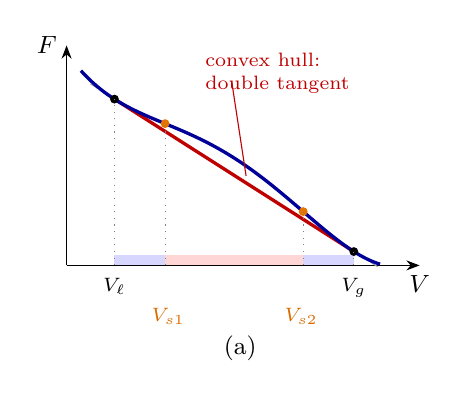
\begin{tikzpicture}[>=Stealth,font=\small,x=1.52cm,y=0.44cm]
  \draw[->] (0.60,0) -- (3.55,0) node[below]{$V$};
  \draw[->] (0.60,0) -- (0.60,6.35) node[left]{$F$};
  % unstable / metastable shading bands on the axis
  \fill[red!16] (1.423,0) rectangle (2.577,0.30);
  \fill[blue!16] (1.0,0) rectangle (1.423,0.30);
  \fill[blue!16] (2.577,0) rectangle (3.0,0.30);
  % double tangent (convex hull), extended dashed
  \draw[dashed,gray!70] (0.80,{7-2.2*0.80}) -- (3.22,{7-2.2*3.22});
  \draw[very thick,red!75!black] (1.0,4.8) -- (3.0,0.4);
  % F(V)
  \draw[very thick,blue!60!black,domain=0.72:3.22,samples=90,smooth,variable=\x]
       plot ({\x},{0.5*((\x-2)*(\x-2)-1)*((\x-2)*(\x-2)-1)-2.2*\x+7});
  \fill (1.0,4.8) circle (1.6pt);
  \fill (3.0,0.4) circle (1.6pt);
  \fill[orange!90!black] (1.423,4.092) circle (1.6pt);
  \fill[orange!90!black] (2.577,1.553) circle (1.6pt);
  \draw[dotted,gray] (1.0,0) -- (1.0,4.8);
  \draw[dotted,gray] (3.0,0) -- (3.0,0.4);
  \draw[dotted,gray] (1.423,0) -- (1.423,4.092);
  \draw[dotted,gray] (2.577,0) -- (2.577,1.553);
  \node[anchor=north,font=\scriptsize] at (1.0,-0.10) {$V_\ell$};
  \node[anchor=north,font=\scriptsize] at (3.0,-0.10) {$V_g$};
  \node[anchor=north,font=\scriptsize,orange!85!black] at (1.45,-0.95) {$V_{s1}$};
  \node[anchor=north,font=\scriptsize,orange!85!black] at (2.56,-0.95) {$V_{s2}$};
  \node[anchor=west,font=\scriptsize,red!75!black,align=left,inner sep=1.5pt]
       at (1.72,5.55) {convex hull:\\ double tangent};
  \draw[red!75!black,thin] (1.98,5.30) -- (2.10,2.58);
  \node[anchor=north,font=\small] at (2.05,-1.75) {(a)};
\end{tikzpicture}
\hfill
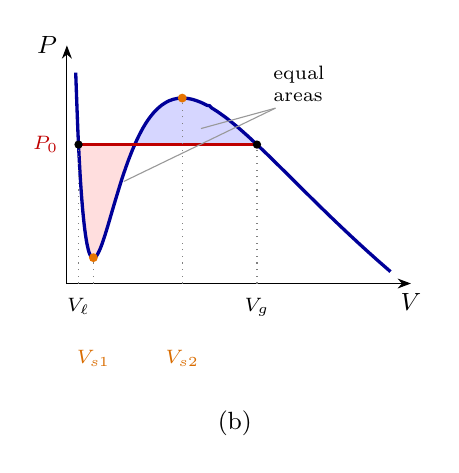
\begin{tikzpicture}[>=Stealth,font=\small,x=1.72cm,y=0.96cm]
  \def\vdw{12*(7.44/(3*\x-1)-3/(\x*\x)-0.59)}
  \fill[red!13,domain=0.6459:1.0610,samples=60,smooth,variable=\x]
       plot ({\x},{\vdw}) -- cycle;
  \fill[blue!16,domain=1.0610:1.9634,samples=60,smooth,variable=\x]
       plot ({\x},{\vdw}) -- cycle;
  \draw[->] (0.56,0) -- (3.10,0) node[below]{$V$};
  \draw[->] (0.56,0) -- (0.56,3.15) node[left]{$P$};
  \draw[very thick,blue!60!black,domain=0.625:2.95,samples=140,smooth,variable=\x]
       plot ({\x},{\vdw});
  \draw[very thick,red!75!black] (0.6459,1.838) -- (1.9634,1.838);
  \draw[dotted,gray] (0.6459,0) -- (0.6459,1.838);
  \draw[dotted,gray] (1.9634,0) -- (1.9634,1.838);
  \draw[dotted,gray] (0.7556,0) -- (0.7556,0.342);
  \draw[dotted,gray] (1.4117,0) -- (1.4117,2.453);
  \fill (0.6459,1.838) circle (1.5pt);
  \fill (1.9634,1.838) circle (1.5pt);
  \fill[orange!90!black] (0.7556,0.342) circle (1.6pt);
  \fill[orange!90!black] (1.4117,2.453) circle (1.6pt);
  \node[anchor=east,font=\scriptsize,red!75!black,inner sep=2pt] at (0.54,1.838) {$P_0$};
  \node[anchor=north,font=\scriptsize] at (0.6459,-0.06) {$V_\ell$};
  \node[anchor=north,font=\scriptsize] at (1.9634,-0.06) {$V_g$};
  \node[anchor=north,font=\scriptsize,orange!85!black] at (0.7556,-0.76) {$V_{s1}$};
  \node[anchor=north,font=\scriptsize,orange!85!black] at (1.4117,-0.76) {$V_{s2}$};
  \node[anchor=south west,font=\scriptsize,align=left,inner sep=1.5pt] at (2.05,2.35)
       {equal\\ areas};
  \draw[thin,gray!80] (2.10,2.32) -- (1.55,2.05);
  \draw[thin,gray!80] (2.10,2.32) -- (0.98,1.35);
  \node[anchor=north,font=\small] at (1.8,-1.55) {(b)};
\end{tikzpicture}

\vspace{2ex}
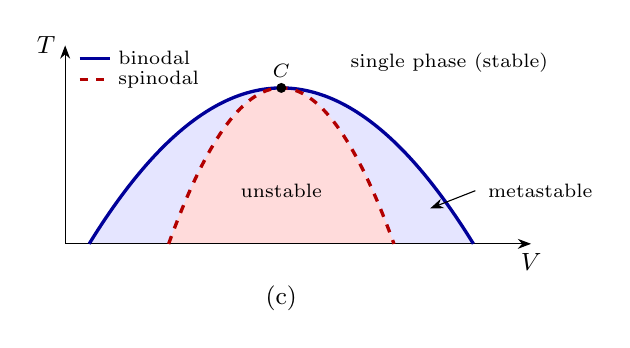
\begin{tikzpicture}[>=Stealth,font=\small,x=1.22cm,y=0.90cm]
  \fill[blue!10] plot[domain=0:4,samples=80,smooth,variable=\x]
       ({\x},{3-0.55*(\x-2)*(\x-2)}) -- (0,0.80) -- cycle;
  \fill[red!14] plot[domain=0.827:3.173,samples=80,smooth,variable=\x]
       ({\x},{3-1.6*(\x-2)*(\x-2)}) -- (0.827,0.80) -- cycle;
  \draw[->] (-0.25,0.80) -- (4.60,0.80) node[below]{$V$};
  \draw[->] (-0.25,0.80) -- (-0.25,3.60) node[left]{$T$};
  \draw[very thick,blue!60!black,domain=0:4,samples=80,smooth,variable=\x]
       plot ({\x},{3-0.55*(\x-2)*(\x-2)});
  \draw[very thick,red!70!black,dashed,domain=0.827:3.173,samples=80,smooth,variable=\x]
       plot ({\x},{3-1.6*(\x-2)*(\x-2)});
  \fill (2,3) circle (1.8pt);
  \node[anchor=south,font=\scriptsize,inner sep=2pt] at (2,3.06) {$C$};
  \node[font=\scriptsize] at (2.0,1.55) {unstable};
  \node[anchor=west,font=\scriptsize] at (4.05,1.55) {metastable};
  \draw[->,thin] (4.02,1.55) -- (3.55,1.30);
  \node[anchor=west,font=\scriptsize] at (2.62,3.35) {single phase (stable)};
  \draw[very thick,blue!60!black] (-0.10,3.42) -- (0.22,3.42);
  \node[anchor=west,font=\scriptsize,inner sep=2pt] at (0.24,3.42) {binodal};
  \draw[very thick,red!70!black,dashed] (-0.10,3.12) -- (0.22,3.12);
  \node[anchor=west,font=\scriptsize,inner sep=2pt] at (0.24,3.12) {spinodal};
  \node[anchor=north,font=\small] at (2.0,0.35) {(c)};
\end{tikzpicture}
\caption{Binodal and spinodal, in the three representations used
interchangeably in the text. \textbf{(a)} The constrained free energy $F(V)$ at
fixed $T<T_c$. The double tangent (red) touches at the \emph{binodal} points
$V_\ell,V_g$; between them the convex hull replaces $F$ by the straight chord,
which lies below the curve, so phase separation genuinely lowers the free energy.
The \emph{spinodal} points $V_{s1},V_{s2}$ (orange) are the inflections where
$\partial^{2}F/\partial V^{2}=0$. The bar on the axis marks the metastable
intervals (blue) and the locally unstable interval (red). \textbf{(b)} The same
isotherm in the $P$--$V$ plane: the horizontal coexistence line $P=P_0$ cuts the
van der Waals loop into two equal-area lobes, and the spinodal points are the
turning points $(\partial P/\partial V)_T=0$. \textbf{(c)} Both loci as curves in
the $T$--$V$ plane. The spinodal (dashed) lies strictly inside the binodal and
touches it only at the critical point $C$. Outside the binodal a uniform state is
the equilibrium state; between binodal and spinodal it is metastable and decays by
nucleation over an exponentially long time; inside the spinodal it is locally
unstable and decays immediately by spinodal decomposition. See
footnotes~\ref{fn:binodal} and \ref{fn:spinodal}.}
\label{fig:binodal}
\end{figure}

Finally, a point that causes recurrent confusion: whether one \emph{picks the
lower minimum} of $F(\phi)$ or \emph{takes the convex
hull}\footnote{\label{fn:hull}\textbf{Convex hull of a function.} For a function
$g$ on an interval, $\operatorname{conv}g$ is the largest convex function that
lies nowhere above $g$; equivalently, the pointwise supremum of all affine
functions $\ell$ with $\ell\leq g$, or the lower boundary of the convex hull (in
the ordinary set-theoretic sense) of the region $\{(x,y):y\geq g(x)\}$ above the
graph. Constructively: stretch a taut string underneath the graph and let it pull
tight. Where $g$ is already convex the string lies on the graph and
$\operatorname{conv}g=g$; where it is not, the string bridges the offending piece
as a straight chord touching at two points --- the double tangent, whose contact
points are the binodal (footnote~\ref{fn:binodal}) and whose chord is the tie
line. Two properties are used in the main text: $\operatorname{conv}g$ is the
largest convex minorant, so $\operatorname{conv}g\leq g$ everywhere with equality
off the chord; and $g^{\ast\ast}=\operatorname{conv}g$, i.e.\ applying the
Legendre--Fenchel transform twice returns not $g$ but its convex hull, which is
exactly why transforming to the field ensemble and back performs the Maxwell
construction automatically. Note also what the hull \emph{destroys}: the barrier
between the wells, and with it every metastable and unstable state, since those
lie strictly above the hull.} depends on the ensemble, not on the physics. If the conjugate field is controlled (magnetic
field $h$ fixed), one minimises $F(\phi)-h\phi$ and simply selects the deeper
well. If the order parameter itself is conserved and controlled (density,
alloy composition, total magnetisation), the accessible states include mixtures
and one takes the hull, obtaining a coexistence region. This is the same
Legendre-transform bookkeeping as everywhere else: $U^{\ast\ast}=\operatorname{conv}U$
means that transforming to the field ensemble and back automatically performs the
Maxwell construction and erases the metastable and unstable branches.

\subsection{Convexity, stability, and response functions}
\label{sec:convexity}

\subsubsection*{Why a Legendre transform flips convexity}

Take the variational form $F(T)=\inf_S[U(S)-TS]$ and read it as a function of $T$
at fixed $S$: the bracket is \emph{affine} (a straight line) in $T$, with slope
$-S$ and intercept $U(S)$. So $F(T)$ is the pointwise infimum of a family of
straight lines. A pointwise infimum of affine functions is concave --- draw two
lines and take the lower envelope --- regardless of the family. Hence:
\[
\boxed{\;F(T)=\inf_S\big[\underbrace{U(S)-TS}_{\text{affine in }T}\big]
\;\Longrightarrow\;F\ \text{concave in}\ T\;}
\]
Symmetrically, $U(S)=\sup_T[F(T)+TS]$ is a supremum of affine functions of $S$
and is therefore convex, which is also why the double transform returns the
convex hull and nothing more. This one-line argument is the whole reason
convexity in a variable becomes concavity in its conjugate; no differentiability
is needed.

For smooth functions there is a differential version that says slightly more.
With $T=U'(S)$ and $S=-F'(T)$,
\[
\frac{\partial^{2}F}{\partial T^{2}}=-\frac{dS}{dT}
=-\left(\frac{dT}{dS}\right)^{-1}
=-\left(\frac{\partial^{2}U}{\partial S^{2}}\right)^{-1}.
\]
The curvatures are not merely opposite in sign but \emph{reciprocal}. Physically
this is a fluctuation statement: a potential that is very flat in $T$ (large
$|F''|$, large $C_V$) corresponds to a fundamental relation that is very stiff in
$S$, and vice versa. A stiff system has small fluctuations of the conjugate
variable.

\subsubsection*{Consequences}

Applying the rule variable by variable: $U$ is convex in all of $S,V,N$; $F$ is
concave in $T$ and convex in $V$; $G$ is concave in both $T$ and $P$; $\Omega$ is
concave in both $T$ and $\mu$. Concavity in $T$ is exactly
\[
\left(\frac{\partial^2F}{\partial T^2}\right)_{V,N}\leq 0
\quad\Longleftrightarrow\quad
C_V=-T\left(\frac{\partial^2F}{\partial T^2}\right)_{V,N}\geq 0,
\]
and convexity in $V$ gives $\kappa_T \geq 0$. These are not accidents: a negative
heat capacity would mean a fluctuation that removes energy raises the
temperature, driving further energy loss --- the equilibrium would be unstable.
Since (Section~\ref{sec:canonical}) these same second derivatives equal
variances, and variances are non-negative, statistical mechanics guarantees
thermodynamic stability automatically. The general pattern,
\[
\text{curvature of potential} \;=\; \text{response function} \;=\;
\text{variance of the conjugate fluctuating quantity},
\]
is the elementary form of the fluctuation--dissipation theorem, and is the reason
response measurements diagnose phase transitions: a diverging susceptibility is a
diverging fluctuation is a vanishing curvature of the free energy.

\section{Statistical ensembles and their partition functions}
\label{sec:ensembles}

Each ensemble corresponds to a choice of which variables the environment fixes,
and computes the corresponding potential as (minus $k_BT$ times) the logarithm of
a partition function. We define all four explicitly before using them.

\paragraph{Microcanonical multiplicity $W$.} For an isolated system,
\[
W(E,V,N)=\#\{\text{microstates with energy in }[E,E+\delta E]\},
\]
sometimes written $g$ or $\Gamma$. Then
\[
\boxed{\;S=k_B\ln W\;}
\]

\paragraph{Canonical partition function $Z$.} System exchanging energy with a
bath at temperature $T$, at fixed $N$ and $V$:
\[
Z(T,V,N)=\sum_i e^{-\beta E_i}=\Tr\, e^{-\beta \hat H},
\qquad p_i=\frac{e^{-\beta E_i}}{Z},
\]
and
\[
\boxed{\;F=-k_BT\ln Z\;}
\]

\begin{remark}[At fixed $T$, does $S$ fluctuate?]
The natural guess --- ``$T$ is fixed, so its conjugate $S$ must fluctuate, and
only $\langle S\rangle$ is defined'' --- is a good instinct applied to the wrong
variable, and the correction is worth making because it clarifies what entropy is.

\emph{What actually fluctuates is $E$, not $S$.} In the canonical ensemble the
fixed quantities are $(T,V,N)$ and the fluctuating one is the energy, with
$\Var(E)=k_BT^{2}C_V$. The conjugate pairing that governs the \emph{ensemble} is
$(\beta,E)$: $\beta$ is the Lagrange multiplier and $E$ is the constrained
quantity it was introduced to control. The pairing $(T,S)$ is a pairing of the
\emph{thermodynamic potential} --- it says $S=-(\partial F/\partial T)_{V,N}$ ---
and the two need not, and do not, coincide.

\emph{Entropy is not an observable.} There is no Hermitian operator $\hat S$
whose expectation value is the thermodynamic entropy. $S=-k_B\Tr(\rho\ln\rho)$ is
a functional of the \emph{distribution} $\rho$, not a function on phase space or
an operator on Hilbert space; it is a property of the ensemble as a whole rather
than of any microstate. Asking for its fluctuation is therefore a category error
in the same way as asking for the fluctuation of the mean of a distribution. The
thermodynamic $S(T,V,N)$ is a definite number, computed from $F$, not an average
of anything.

\emph{The nearest thing that does fluctuate.} One can define a fluctuating
\emph{surprisal} $s_i\equiv-k_B\ln p_i$, whose ensemble average is $S$ by
construction. In the canonical ensemble $p_i=e^{-\beta E_i}/Z$, so
\[
s_i=k_B\big(\beta E_i+\ln Z\big),
\]
which is an \emph{affine} function of $E_i$. Its fluctuations are therefore
nothing but energy fluctuations in disguise:
\[
\Var(s)=k_B^{2}\beta^{2}\Var(E)=k_B^{2}\beta^{2}\,k_BT^{2}C_V=k_B\,C_V .
\]
So the relative spread is $\sqrt{\Var(s)}/S=\sqrt{k_BC_V}/S\sim N^{-1/2}$: sharp in
the thermodynamic limit, exactly like every other extensive quantity. The same
answer comes from the microcanonical route --- treating $S(E)=k_B\ln W(E)$ as a
function of the fluctuating $E$ and linearising, $\delta S\approx\delta E/T$, gives
$\Var(S)\approx\Var(E)/T^{2}=k_BC_V$ --- which is a useful consistency check on
the two pictures.

So: at fixed $T$ the entropy is not a fluctuating quantity whose mean happens to
be quoted. It is a sharp function of $(T,V,N)$; and the surrogate that \emph{can}
be made to fluctuate carries no information beyond the energy fluctuation already
accounted for.
\end{remark}

\paragraph{Grand partition function $\Xi$.} System exchanging both energy and
particles with a reservoir at temperature $T$ and chemical potential $\mu$, at
fixed $V$. Summing over all particle numbers $N$ and, for each, over the
$N$-particle eigenstates $i$ with energies $E_{i,N}$:
\[
\boxed{\;\Xi(T,V,\mu)=\sum_{N=0}^{\infty}\sum_i e^{-\beta(E_{i,N}-\mu N)}
=\sum_{N=0}^{\infty} z^N Z(T,V,N)\;}
\]
where $z=e^{\beta\mu}$ is the fugacity, with probabilities
$p_{i,N}=e^{-\beta(E_{i,N}-\mu N)}/\Xi$, and
\[
\boxed{\;\Omega=-k_BT\ln\Xi\;}
\]

\begin{remark}[Why $-\mu N$, when $U=TS-PV+\mu N$ carries $+\mu N$?]
There is no inconsistency; the two signs answer different questions, and both are
forced.

\emph{The sign in $\Omega$ is the Legendre convention.} A Legendre transform
always \emph{subtracts} the product of the conjugate pair being traded away,
whatever sign that product happens to carry inside $U$. Going from $U(S,V,N)$ to
$F(T,V,N)$ one subtracts $TS$ even though $U$ contains $+TS$, obtaining, by Euler,
$F=U-TS=-PV+\mu N$. Trading $N$ for $\mu$ as well subtracts $\mu N$ in exactly the
same way:
\[
\Omega=F-\mu N=U-TS-\mu N=(TS-PV+\mu N)-TS-\mu N=-PV .
\]
The rule is fixed by requiring that the new potential's differential contain
$-N\,d\mu$ rather than $\mu\,dN$: $d\Omega=dF-\mu\,dN-N\,d\mu=-S\,dT-P\,dV-N\,d\mu$,
which is the whole point of the transform. Reading $+\mu N$ in Euler's relation as
though it dictated the sign of the transform conflates the \emph{value} of $U$
with the \emph{operation} performed on it.

\emph{The sign in the Boltzmann weight is forced by the reservoir's entropy.}
This is the more physical statement, and it is a two-line derivation. The system
and reservoir together are isolated with total energy $E_{\rm tot}$ and total
particle number $N_{\rm tot}$. If the system occupies a definite microstate with
energy $E$ and particle number $N$, the number of composite microstates is just
the reservoir's, so
\[
p_{i,N}\ \propto\ W_{\rm res}(E_{\rm tot}-E,\,N_{\rm tot}-N)
=\exp\!\Big[\tfrac{1}{k_B}S_{\rm res}(E_{\rm tot}-E,\,N_{\rm tot}-N)\Big].
\]
Expanding to first order in the small quantities $E$ and $N$, and using the
reservoir's own equations of state $(\partial S/\partial E)_{V,N}=1/T$ and
$(\partial S/\partial N)_{E,V}=-\mu/T$,
\[
S_{\rm res}(E_{\rm tot}-E,N_{\rm tot}-N)
=S_{\rm res}(E_{\rm tot},N_{\rm tot})-\frac{E}{T}+\frac{\mu N}{T}+\dots ,
\]
so that
\[
p_{i,N}\ \propto\ e^{-\beta(E-\mu N)} .
\]
The relative minus sign between $E$ and $\mu N$ traces directly to the relative
minus sign between $1/T$ and $-\mu/T$ in the reservoir's derivatives --- i.e.\ to
the fact that giving the system a particle \emph{costs} the reservoir energy but
\emph{relieves} it of a particle. The physics is visible in the result: raising
$\mu$ multiplies the weight of an $N$-particle state by $e^{+\beta\mu N}$ and so
favours large $N$, which is what a large chemical potential is supposed to do.
Had the sign been $+\mu N$ in the exponent, a high chemical potential would empty
the system.
\end{remark}

\begin{remark}[Adding magnetisation: $\mathcal{H}\,dM$ or $M\,d\mathcal{H}$?]
Both, in different potentials --- and the pattern is exactly the one just
described for $(\mu,N)$, with the total magnetisation $M$ playing the role of $N$
and the applied field $\mathcal{H}$ that of $\mu$. (The script
$\mathcal{H}$ avoids a collision: $H$ is the enthalpy and $\hat H$ the
Hamiltonian. In the density notation of
Section~\ref{sec:criticalnonanalytic}, $h=\mathcal{H}$ and $m=M/V$.)

\emph{In the energy representation, $\mathcal{H}\,dM$.} $M$ is extensive and
$\mathcal{H}$ intensive, so $M$ joins $(S,V,N)$ as a natural variable of $U$, and
the work done \emph{on} the system in magnetising it is
$\dbar W=\mathcal{H}\,dM$:
\[
U=U(S,V,N,M),\qquad
dU=T\,dS-P\,dV+\mu\,dN+\mathcal{H}\,dM .
\]
The Euler relation acquires a term likewise, $U=TS-PV+\mu N+\mathcal{H}M$, and
Gibbs--Duhem becomes $S\,dT-V\,dP+N\,d\mu+M\,d\mathcal{H}=0$. The pair
$(\mathcal{H},M)$ is the magnetic analogue of $(\mu,N)$ --- and note why
$\mathcal{H}\,dM$ carries the opposite sign to $-P\,dV$: magnetising a sample
against a field costs energy, whereas expanding against a pressure releases it.

\emph{In the field-controlled potential, $-M\,d\mathcal{H}$.} An experiment fixes
$\mathcal{H}$, not $M$, so one Legendre transforms, subtracting the product as
always:
\[
\tilde F(T,V,N,\mathcal{H})=F-\mathcal{H}M,
\qquad
d\tilde F=-S\,dT-P\,dV+\mu\,dN-M\,d\mathcal{H} ,
\]
whence $M=-(\partial\tilde F/\partial\mathcal{H})_{T,V,N}$ and
$\chi=-(\partial^{2}\tilde F/\partial\mathcal{H}^{2})_{T,V,N}\geq0$: another
instance of curvature $=$ response $=$ variance.

\emph{In the partition function, $-\mathcal{H}M$ in the exponent.} Fixing
$\mathcal{H}$ means fixing an intensive variable and letting its extensive partner
fluctuate, so the construction is verbatim that of $\Xi$:
\[
\mathcal{Z}(T,V,N,\mathcal{H})=\sum_{i}e^{-\beta(E_{i}-\mathcal{H}M_{i})}
=\Tr\,e^{-\beta(\hat H-\mathcal{H}\hat M)},
\qquad
\tilde F=-k_BT\ln\mathcal{Z},
\]
with the same minus sign and for the same reason --- it is the field source's
entropy bookkeeping that supplies it --- and consequently
$\Var(M)=k_BT\,\chi$, exactly parallel to
$\Var(N)=k_BT\,(\partial N/\partial\mu)_{T,V}$.

So the short answer to ``$\mathcal{H}\,dM$ or $M\,d\mathcal{H}$?'' is: the
extensive-variable form $\mathcal{H}\,dM$ in $dU$, $dH$, $dF$, $dG$; the
transformed form $-M\,d\mathcal{H}$ in whichever potential has traded $M$ away.
Which one is correct is decided by which quantity the apparatus holds fixed, not
by preference.

Two cautions. First, the division of magnetic work between ``the sample'' and
``the field in the volume it occupies'' is convention-dependent, and $\mathcal{H}$
versus $B$ versus $\mu_0\mathcal{H}$ differ by exactly such terms; the form above
is the one in which $M$ is the sample's moment and $\mathcal{H}$ the applied
field, which is what experiments report. Second, ferromagnets are precisely where
hysteresis makes $U$ multivalued --- assumption (A1) of
Section~\ref{sec:totaldiff} --- so the relations above hold on the equilibrium
branch, not around a loop.
\end{remark}
Consistency check: since $\Omega=-PV$, this says $\ln\Xi=\beta PV$. The symbol
$\Xi$ is a capital Greek xi, chosen to avoid the already-overloaded $\Omega$.

\paragraph{Isothermal--isobaric partition function $\Delta$.} System exchanging
energy \emph{and volume} with a reservoir at temperature $T$ and pressure $P$, at
fixed $N$. Volume is now a fluctuating variable and the Boltzmann weight acquires
the mechanical work term $PV$:
\[
\boxed{\;\Delta(T,P,N)=\sum_V e^{-\beta PV}Z(T,V,N)
\;\xrightarrow[\text{continuum}]{}\;
\frac{1}{V_0}\int_0^\infty\! dV\, e^{-\beta PV}Z(T,V,N)\;}
\]
and
\[
\boxed{\;G=-k_BT\ln\Delta\;}
\]
Some authors write $Z_{NPT}$, $Y$, or $\Delta_N$ for the same object. The
reference volume $V_0$ makes the integral dimensionless; it contributes a term of
order $\ln V$ to $G$, which is subextensive and therefore irrelevant in the
thermodynamic limit. Consistency check: $G=\mu N$ gives $\ln\Delta=-\beta\mu N$.
This ensemble is the natural one for constant-pressure molecular dynamics
simulations.

\paragraph{Summary.}
\begin{center}
\begin{tabular}{llll}
\toprule
Ensemble & Fixed & Fluctuating & Potential \\
\midrule
Microcanonical & $E,V,N$ & --- & $S=k_B\ln W$ \\
Canonical & $T,V,N$ & $E$ & $F=-k_BT\ln Z$ \\
Grand canonical & $T,V,\mu$ & $E,N$ & $\Omega=-k_BT\ln\Xi$ \\
Isothermal--isobaric & $T,P,N$ & $E,V$ & $G=-k_BT\ln\Delta$ \\
\bottomrule
\end{tabular}
\end{center}

The pattern is a Legendre transform on the thermodynamic side matched by a
Laplace transform on the statistical side: $Z=\sum_E W e^{-\beta E}$,
$\Xi=\sum_N Z e^{\beta\mu N}$, $\Delta=\sum_V Z e^{-\beta PV}$. Evaluating each
Laplace transform by steepest descent in the thermodynamic limit reproduces the
Legendre transform exactly, with the saddle point at the equilibrium value of the
fluctuating variable and the Gaussian width around it giving its variance.

\section{Ensemble equivalence and its limits}
\label{sec:equivalence}

\subsection{Why the potentials agree}

Take $\Xi=\sum_N e^{-\beta[F(T,V,N)-\mu N]}$ and evaluate by steepest descent.
The exponent is stationary at $N^\ast$ satisfying $(\partial F/\partial
N)_{T,V}=\mu$, which is the thermodynamic condition for particle equilibrium with
the reservoir. Expanding to second order,
\[
\Xi\simeq e^{-\beta[F(N^\ast)-\mu N^\ast]}
\int\! dN\,e^{-\tfrac{\beta}{2}F''(N^\ast)(N-N^\ast)^2}
= e^{-\beta\Omega_{\rm saddle}}\sqrt{\frac{2\pi}{\beta F''}} ,
\]
so
\[
\Omega=-k_BT\ln\Xi=\underbrace{F(N^\ast)-\mu N^\ast}_{\text{Legendre transform}}
\;+\;\mathcal{O}(\ln N).
\]
Since $F''=(\partial\mu/\partial N)_{T,V}\sim1/N$, the Gaussian has
$\Var(N)=k_BT/F''\sim N$, i.e.\ $\Delta N/N\sim N^{-1/2}$, and the correction to
$\Omega$ is $\mathcal{O}(\ln N)$: subextensive, hence invisible in the densities
$\omega=\Omega/V$. \textbf{This is the whole content of ensemble equivalence: the
two ensembles produce the same thermodynamic surface, up to subextensive terms.}

\subsection{Why response functions at fixed intensive variable nevertheless differ}
\label{sec:respdiffer}

Here is the point that the $N^{-1/2}$ slogan obscures. Ensemble equivalence
states that the \emph{function} $S(T,V,\mu)$, or equivalently the fundamental
relation, is the same in both descriptions. A response function, however, is not
determined by the surface alone: it is a \emph{directional derivative}, determined
by the surface \emph{and} the direction of differentiation. Fixing $\mu$ and
fixing $N$ define two different curves through the same point of the same surface,
so
\[
C_{V,N}=T\left(\frac{\partial S}{\partial T}\right)_{V,N}
\qquad\text{and}\qquad
C_{V,\mu}=T\left(\frac{\partial S}{\partial T}\right)_{V,\mu}
\]
are simply two different numbers, exactly as $C_P\neq C_V$ within a single
ensemble. Nobody calls $C_P\neq C_V$ an ensemble inequivalence, and the present
case is no different.

The size of the difference is worth tracking, because it is \emph{not} a
$1/N$ correction. From Section~\ref{sec:caveat},
\[
C_{V,\mu}-C_{V,N}=T\,\frac{\big[(\partial N/\partial T)_{V,\mu}\big]^{2}}
{(\partial N/\partial\mu)_{T,V}} .
\]
Both derivatives are extensive: $(\partial N/\partial T)_{V,\mu}=\mathcal{O}(N)$
and $(\partial N/\partial\mu)_{T,V}=\beta\Var(N)=\mathcal{O}(N)$. So the
difference is $\mathcal{O}(N^{2}/N)=\mathcal{O}(N)$ --- the same order as the heat
capacities themselves. The resolution of the apparent paradox is that
$N^{-1/2}$ refers to \emph{relative} fluctuations. Response functions are built
from the \emph{absolute} fluctuations, which are extensive and do not go away.
Saying $\Delta N/N\to0$ is not saying $\Var(N)\to0$.

\subsection{Genuine inequivalence at a first-order transition}
\label{sec:firstorder}

Here equivalence really does fail, and the mechanism is the Maxwell construction
of Section~\ref{sec:maxwell} transplanted to energy space.

At a temperature-driven first-order transition there is a latent heat, so the
ordered and disordered phases have \emph{different} energy densities $e_o\neq e_d$
at the same transition temperature $T_t$. Since the two phases have equal free
energy at $T_t$, they carry equal canonical weight, and the canonical energy
distribution
\[
P(E)\;\propto\;W(E)\,e^{-\beta E}\;=\;e^{[S(E)-E/T]/k_B}
\]
has \textbf{two peaks}, at $E=Ve_o$ and $E=Ve_d$, separated by a minimum. The dip
between them is the free-energy cost of the interface between coexisting phases,
so the barrier scales as
\[
\Delta F(L)=\ln\frac{P_{\max}}{P_{\min}}\;\sim\;2\sigma L^{d-1},
\]
with $\sigma$ the interfacial tension. This is the Lee--Kosterlitz criterion, and
it is the standard numerical diagnostic for the order of a transition: a barrier
that \emph{grows} with $L$ signals first order, whereas one that stays constant
signals a continuous transition (Section~\ref{sec:fss:firstorder} places it
alongside the other finite-size discriminants). It is also why multicanonical and Wang--Landau
sampling were invented --- ordinary Metropolis dynamics cannot cross the barrier.

The inequivalence follows immediately. Microcanonically, all energies between
$Ve_o$ and $Ve_d$ are perfectly accessible; they are phase-separated
configurations containing an interface. Canonically they are exponentially
suppressed and never typical. In the thermodynamic limit $s(e)$ is \emph{linear}
across that interval (at finite $L$ it has a ``convex intruder'', giving a
negative microcanonical specific heat), so the Legendre transform $s\mapsto f$ is
not invertible there: an entire interval of $e$ maps to the single temperature
$T_t$. The canonical ensemble cannot resolve which $e$; the microcanonical can.
Microcanonical is strictly finer, and information is genuinely lost. The
linear segment of $s(e)$ is the exact analogue of the flat portion of the convex
hull of $F(V)$, and the correspondence is not an analogy but the same theorem.

\begin{warning}[Energy distribution versus order-parameter distribution]
It is easy to conflate two different histograms here, and they behave oppositely.
The modality of each is not a rule of thumb but a consequence of one principle,
so it is worth deriving rather than tabulating.

\paragraph{The principle.} Both histograms are large-deviation distributions of
the form
\[
P(x)\;\propto\;e^{-V\varphi(x)/k_BT} ,
\]
with $\varphi$ a \emph{constrained} free-energy density in the sense of
Section~\ref{sec:minimum}, and $V$ the volume. As $V\to\infty$ the distribution
concentrates on the global minima of $\varphi$, and around each one it is Gaussian
with a width set by the local curvature. Hence
\[
\boxed{\;\#\ \text{peaks of }P(x)\;=\;\#\ \text{degenerate global minima of }
\varphi(x)\;}
\]
Everything below is this statement applied twice, once with $x=E$ and once with
$x=\phi$. Nothing is postulated about ``binary'' order parameters.

\paragraph{$P(E)$: count the distinct energy densities of the coexisting phases.}
Write $E=Ve$ and use $S=k_B\ln W$:
\[
P(e)\;\propto\;W(E)\,e^{-\beta E}
=\exp\!\left[\frac{V}{k_B}\Big(s(e)-\frac{e}{T}\Big)\right],
\]
so $\varphi\propto -\big(s(e)-e/T\big)$ and the maxima solve
\[
s'(e)=\frac{1}{T}
\qquad\text{i.e.}\qquad
T(e)=T .
\]
Now use the concavity of $s(e)$ established in Section~\ref{sec:whyconvex}:
\begin{itemize}
\item \emph{Away from a first-order transition, $s$ is strictly concave}, so $s'$
is strictly decreasing and $s'(e)=1/T$ has exactly one root. \textbf{One peak, at
every temperature} --- including at $T_c$. Expanding around the root gives
\[
\Var(E)=-\frac{Vk_B}{s''(e^{\ast})}=Vk_BT^{2}c=k_BT^{2}C ,
\]
recovering the canonical result. At a continuous transition $c\to\infty$, so
$s''(e^{\ast})=-1/(T^{2}c)\to0$: the curvature vanishes \emph{at a single point}
without $s$ acquiring a flat interval. A vanishing curvature at one point widens
the peak; only a flat interval can split it. This is the precise sense in which
$P(E)$ ``broadens anomalously but does not split'': $\Var(E)\sim
L^{d+\alpha/\nu}$ rather than $L^{d}$, while the \emph{density} still sharpens,
$\sqrt{\Var(e)}\sim L^{(\alpha/\nu-d)/2}\to0$.
\item \emph{At a first-order transition $s$ has a straight segment} of slope
$1/T_t$ joining $e_o$ to $e_d$ (Section~\ref{sec:firstorder}). At $T=T_t$ the
exponent $s(e)-e/T_t$ is therefore \emph{constant} across the whole segment: to
leading order in $V$ the maximum is degenerate along an interval, not at two
points. The degeneracy is lifted at the next order. Any configuration with $e$
strictly inside the interval is a phase-separated one and must contain an
interface, whose free-energy cost is $2\sigma L^{d-1}$ --- subextensive, hence
invisible in $s(e)$, but a genuine \emph{penalty} on the interior:
\[
\ln P(e)=\frac{V}{k_B}\Big(s(e)-\frac{e}{T_t}\Big)
-\frac{2\sigma L^{d-1}}{k_BT_t}\Big|_{\text{interior}}+\dots
\]
The two endpoints, being single-phase and interface-free, escape the penalty.
Hence \textbf{exactly two peaks}, at $e_o$ and $e_d$, and the dip between them has
depth $\ln(P_{\max}/P_{\min})\simeq2\sigma L^{d-1}/k_BT_t$ --- which is precisely
the Lee--Kosterlitz barrier quoted above, now derived rather than asserted.
\end{itemize}
The count is therefore the number of \emph{distinct energy densities} among the
coexisting phases. Note the consequence for symmetric models: at a first-order
transition of the $q$-state Potts model the $q$ ordered states are related by
symmetry and so share one energy density $e_o$, giving $P(E)$ \textbf{two} peaks,
not $q+1$.

\paragraph{$P(\phi)$: count the degenerate minima, which means count the broken
symmetry.} Here $\varphi$ is the constrained free-energy density $f(T;\phi)$ of
Section~\ref{sec:minimum}, defined by the restricted trace
$e^{-\beta Vf(\phi)}=\Tr\big[\delta(\hat\phi-\phi)e^{-\beta\hat H}\big]$, so that
literally $P(\phi)\propto e^{-\beta Vf(\phi)}$ and the histogram \emph{is} the
constrained free energy. The number of peaks is then a group-theoretic question,
not an empirical one. If the Hamiltonian is invariant under a symmetry group $G$
and the ordered state is invariant only under a subgroup $H\subset G$, the set of
degenerate minima is the coset space $G/H$ --- the order-parameter manifold ---
and
\[
\#\ \text{ordered peaks}=|G/H| .
\]
This immediately answers the question of what happens when the order parameter is
not binary:
\begin{itemize}
\item \textbf{Ising, $G=\mathbb{Z}_2$}, $H=\{e\}$: $|G/H|=2$, peaks at $\pm m_s$.
\emph{This} is where ``bimodal'' comes from. It is a fact about
$\mathbb{Z}_2$, not a general truth.
\item \textbf{$q$-state Potts or $\mathbb{Z}_q$ clock, $T<T_c$}: $q$ degenerate
ordered states, hence \textbf{$q$ peaks}. For $q=3$ these sit at the vertices of
a triangle in the two-component order-parameter plane.
\item \textbf{XY, $G=U(1)$}: $G/H$ is a \emph{circle}. There are no discrete
peaks at all --- $P(\mathbf{m})$ is supported on a degenerate ring
$|\mathbf{m}|=m_s$ with the phase free. Beware: the marginal distribution of a
single component $m_x$ is double-peaked, which is a projection artifact and not
two phases.
\item \textbf{Heisenberg, $G=O(3)$}: $G/H=S^{2}$, a spherical shell of maxima.
\item \textbf{$T>T_c$}: $f$ has a single minimum at $\phi=0$; one peak.
\item \textbf{$T=T_c$ exactly}: $f$ is flat to quartic order at the fixed point
and the concentration argument fails, since the correlation length is comparable
to $L$. $P(\phi)$ is then the \emph{universal critical distribution}, a broad,
weakly double-humped shape --- neither the two sharp peaks of $T<T_c$ nor the
single Gaussian of $T>T_c$. Its shape is a universal function, and its fourth
cumulant is what the Binder crossing below exploits.
\item \textbf{Symmetry-breaking first-order transition at $T_t$} (Potts with
$q>4$ in $d=2$, $q\geq3$ in $d=3$): the $q$ ordered minima and the disordered
minimum at $\phi=0$ are \emph{all} degenerate in free energy at $T_t$, since that
is what ``the transition temperature'' means. Hence \textbf{$q+1$ peaks}. Two
provisos: this holds only \emph{at} $T_t$ (just off it, one set of minima is
lower and the others are metastable), and only for a first-order transition that
also breaks a symmetry. A first-order transition with no symmetry breaking ---
liquid--gas --- has just \textbf{two} peaks in $P(\rho)$.
\item \textbf{The $q=2$ caveat.} There is no first-order $q=2$ case: the
two-state Potts model \emph{is} the Ising model, whose transition is continuous in
every dimension $d\geq2$. The formula $q+1$ therefore never yields three peaks
for Ising, and one should not read the table as claiming so.
\end{itemize}

\paragraph{The instances, collected.}
\begin{center}
\renewcommand{\arraystretch}{1.15}
\begin{tabular}{lcc}
\toprule
Situation & $P(E)$ & $P(\phi)$ \\
\midrule
Ising, $T>T_c$ & unimodal & unimodal at $\phi=0$ \\
Ising, $T<T_c$ & unimodal & bimodal, $\pm m_s$ \\
Ising, $T=T_c$ & unimodal, anomalously broad & universal double-humped \\
XY / Heisenberg, $T<T_c$ & unimodal & ring $S^{1}$ / shell $S^{2}$ \\
$q$-state Potts, continuous, $T<T_c$ & unimodal & $q$-modal \\
$q$-state Potts, first order, $T=T_t$ & bimodal ($e_o,e_d$) & $(q{+}1)$-modal \\
Liquid--gas, first order, $T=T_t$ & bimodal ($e_\ell,e_g$) & bimodal ($\rho_\ell,\rho_g$) \\
\bottomrule
\end{tabular}
\end{center}
Figure~\ref{fig:histograms} shows the characteristic shapes, and
Appendix~\ref{sec:appising} computes every entry of the Ising rows explicitly in
mean-field theory, where $P(m)$, $P(E)$, $c$, $\chi$ and $U_4$ are all available
in closed form, and Appendix~\ref{sec:apppotts} does the same for the $q$-state
Potts rows, including the $(q{+}1)$-modal $P(\phi)$ and the bimodal $P(E)$.

\paragraph{A finite-size proviso.} All of the multi-peak statements describe the
\emph{equilibrium} distribution. In a finite system the peaks are separated by
barriers $\sim2\sigma L^{d-1}$, so the time to tunnel between them grows as
$e^{2\sigma L^{d-1}/k_BT}$; a simulation that does not cross the barrier will
report one peak regardless. In the thermodynamic limit the barriers are infinite,
the ensemble is non-ergodic, and one must choose a sector by hand --- which is
just spontaneous symmetry breaking, and the same statement as the ensemble
inequivalence of Section~\ref{sec:firstorder}.

\paragraph{Why both facts are used in practice.} Two different cumulants exploit
them. The fourth-order magnetisation cumulant
$U_4=1-\langle\phi^4\rangle/3\langle\phi^2\rangle^2$ takes the value $0$ for a
single Gaussian ($T>T_c$) and $2/3$ for two sharp symmetric peaks ($T<T_c$), so
at $T_c$ it sits at a universal intermediate value and its curves for different
$L$ cross there --- the Binder crossing that locates $T_c$. At a first-order
transition it instead develops a minimum that diverges negatively with $L$,
because the $\phi=0$ peak coexists with the ordered ones. The \emph{energy}
cumulant $V_L=1-\langle E^4\rangle/3\langle E^2\rangle^2$ stays at $2/3$ through a
continuous transition and deviates at a first-order one --- precisely because
$P(E)$ is bimodal there and unimodal here.

\begin{figure}[htbp]
\centering
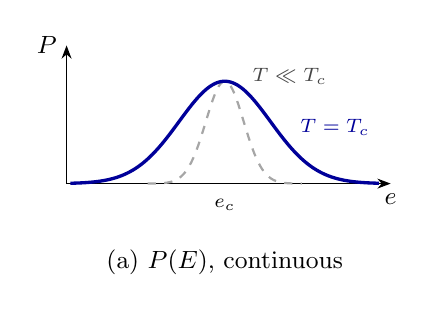
\begin{tikzpicture}[>=Stealth,font=\small,x=0.98cm,y=1.30cm]
  \draw[->] (-2.05,0) -- (2.15,0) node[below]{$e$};
  \draw[->] (-2.05,0) -- (-2.05,1.35) node[left]{$P$};
  \draw[thick,gray!70,dashed,domain=-1.0:1.0,samples=90,smooth,variable=\x]
       plot ({\x},{exp(-\x*\x/0.12)});
  \draw[very thick,blue!60!black,domain=-2:2,samples=110,smooth,variable=\x]
       plot ({\x},{exp(-\x*\x/0.70)});
  \node[anchor=north,font=\scriptsize] at (0,-0.06) {$e_c$};
  \node[anchor=west,font=\scriptsize,gray!55!black,inner sep=1.5pt] at (0.30,1.05) {$T\ll T_c$};
  \node[anchor=west,font=\scriptsize,blue!60!black,inner sep=1.5pt] at (0.92,0.55) {$T=T_c$};
  \node[anchor=north,font=\small] at (0,-0.55) {(a) $P(E)$, continuous};
\end{tikzpicture}
\hfill
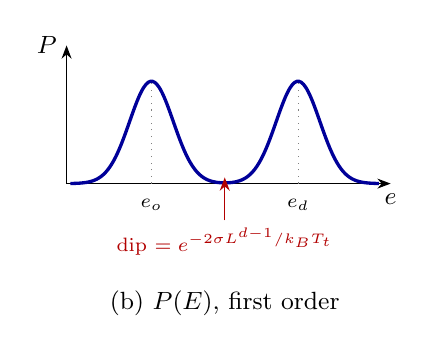
\begin{tikzpicture}[>=Stealth,font=\small,x=0.98cm,y=1.30cm]
  \draw[->] (-2.05,0) -- (2.15,0) node[below]{$e$};
  \draw[->] (-2.05,0) -- (-2.05,1.35) node[left]{$P$};
  \draw[very thick,blue!60!black,domain=-2:2,samples=140,smooth,variable=\x]
       plot ({\x},{exp(-(\x-0.95)*(\x-0.95)/0.16)+exp(-(\x+0.95)*(\x+0.95)/0.16)});
  \draw[dotted,gray] (-0.95,0) -- (-0.95,1.0);
  \draw[dotted,gray] (0.95,0) -- (0.95,1.0);
  \node[anchor=north,font=\scriptsize] at (-0.95,-0.06) {$e_o$};
  \node[anchor=north,font=\scriptsize] at (0.95,-0.06) {$e_d$};
  \node[anchor=north,font=\scriptsize,red!70!black,inner sep=1pt]
       at (0,-0.40) {dip $=e^{-2\sigma L^{d-1}/k_BT_t}$};
  \draw[->,red!70!black,thin] (0,-0.36) -- (0,0.06);
  \node[anchor=north,font=\small] at (0,-0.95) {(b) $P(E)$, first order};
\end{tikzpicture}
\hfill
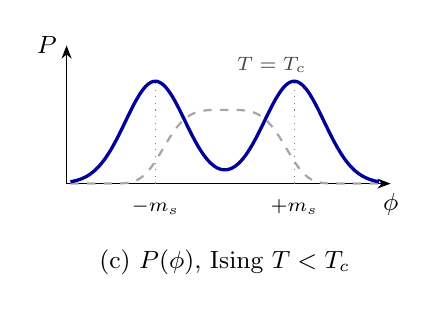
\begin{tikzpicture}[>=Stealth,font=\small,x=0.98cm,y=1.30cm]
  \draw[->] (-2.05,0) -- (2.15,0) node[below]{$\phi$};
  \draw[->] (-2.05,0) -- (-2.05,1.35) node[left]{$P$};
  \draw[thick,gray!70,dashed,domain=-2:2,samples=110,smooth,variable=\x]
       plot ({\x},{0.72*exp(-\x*\x*\x*\x/0.55)});
  \draw[very thick,blue!60!black,domain=-2:2,samples=140,smooth,variable=\x]
       plot ({\x},{exp(-(\x-0.90)*(\x-0.90)/0.30)+exp(-(\x+0.90)*(\x+0.90)/0.30)});
  \draw[dotted,gray] (-0.90,0) -- (-0.90,1.0);
  \draw[dotted,gray] (0.90,0) -- (0.90,1.0);
  \node[anchor=north,font=\scriptsize] at (-0.90,-0.06) {$-m_s$};
  \node[anchor=north,font=\scriptsize] at (0.90,-0.06) {$+m_s$};
  \node[anchor=west,font=\scriptsize,gray!55!black,align=left,inner sep=1.5pt]
       at (0.10,1.16) {$T=T_c$};
  \node[anchor=north,font=\small] at (0,-0.55) {(c) $P(\phi)$, Ising $T<T_c$};
\end{tikzpicture}

\vspace{3ex}
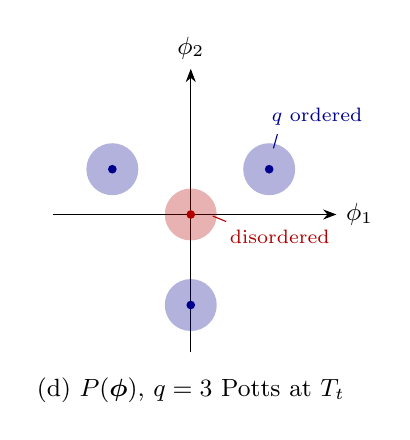
\begin{tikzpicture}[>=Stealth,font=\small,x=1.0cm,y=1.0cm]
  \draw[->] (-1.75,0) -- (1.85,0) node[right]{$\phi_1$};
  \draw[->] (0,-1.75) -- (0,1.85) node[above]{$\phi_2$};
  \foreach \a in {30,150,270}{
     \fill[blue!55!black,opacity=0.30] (\a:1.15) circle (0.33);
     \fill[blue!55!black] (\a:1.15) circle (0.055);}
  \fill[red!70!black,opacity=0.30] (0,0) circle (0.33);
  \fill[red!70!black] (0,0) circle (0.055);
  \node[anchor=south west,font=\scriptsize,blue!55!black,inner sep=2pt] at (0.95,1.05)
       {$q$ ordered};
  \draw[blue!55!black,thin] (1.10,1.02) -- (1.05,0.84);
  \node[anchor=north west,font=\scriptsize,red!70!black,inner sep=2pt] at (0.42,-0.12)
       {disordered};
  \draw[red!70!black,thin] (0.45,-0.09) -- (0.28,-0.02);
  \node[anchor=north,font=\small] at (0,-1.95) {(d) $P(\boldsymbol{\phi})$, $q=3$ Potts at $T_t$};
\end{tikzpicture}
\hspace{0.06\textwidth}
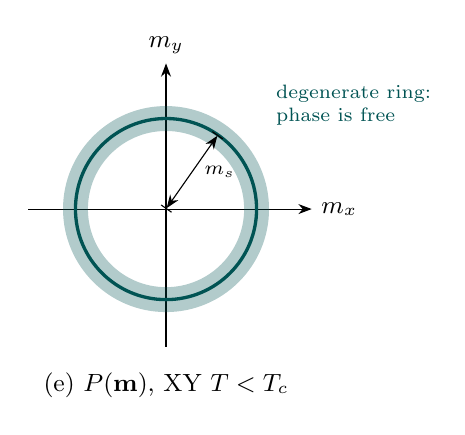
\begin{tikzpicture}[>=Stealth,font=\small,x=1.0cm,y=1.0cm]
  \draw[->] (-1.75,0) -- (1.85,0) node[right]{$m_x$};
  \draw[->] (0,-1.75) -- (0,1.85) node[above]{$m_y$};
  \draw[teal!65!black,opacity=0.30,line width=9pt] (0,0) circle (1.15);
  \draw[very thick,teal!65!black] (0,0) circle (1.15);
  \draw[|<->|,thin] (0,0) -- (55:1.15) node[midway,right=1pt,font=\scriptsize]{$m_s$};
  \node[anchor=west,font=\scriptsize,teal!65!black,align=left,inner sep=2pt]
       at (1.32,1.32) {degenerate ring:\\ phase is free};
  \node[anchor=north,font=\small] at (0,-1.95) {(e) $P(\mathbf{m})$, XY $T<T_c$};
\end{tikzpicture}
\caption{Shapes of the two histograms. \textbf{(a)} At a continuous transition
$P(E)$ stays unimodal at all $T$, because $s(e)$ is strictly concave; at $T_c$ its
curvature vanishes at the single point $e_c$, which broadens the peak
($\Var(E)\sim L^{d+\alpha/\nu}$) without splitting it. \textbf{(b)} At a
first-order transition $s(e)$ is affine between $e_o$ and $e_d$; the interfacial
cost penalises the interior of that interval and leaves exactly two peaks, with a
dip of depth $2\sigma L^{d-1}$ in $\ln P$ --- the Lee--Kosterlitz barrier.
\textbf{(c)}--\textbf{(e)} $P(\phi)$ counts the degenerate minima of the
constrained free energy, i.e.\ the order-parameter manifold $G/H$. For Ising
($\mathbb{Z}_2$) that is two points; at $T_c$ the peaks merge into the universal
critical distribution (dashed). For the $q=3$ Potts model at a first-order $T_t$
it is $q$ ordered states plus the disordered one, $q+1$ maxima in the
two-component plane. For the XY model it is a continuous circle, with no discrete
peaks at all --- ``bimodal'' is a statement about $\mathbb{Z}_2$, not a general
rule.}
\label{fig:histograms}
\end{figure}
\end{warning}

\subsection{Continuous transitions: the potentials agree, the exponents need not}
\label{sec:fisher}

Does equivalence break at higher-order transitions too? At the level of the
potentials, no --- for short-range interactions $s(e)$ remains strictly concave
through a continuous transition, there is no linear segment, the Legendre
transform stays invertible, and both ensembles yield the same free energy. But at
the level of \emph{critical behaviour} the answer is yes, and the effect has a
name: \textbf{Fisher renormalisation}. It is the critical-point face of exactly
the same $C_{V,\mu}$ versus $C_{V,N}$ distinction discussed above.

\paragraph{The mechanism.} Suppose a system has a hidden constraint --- fixed
particle number, fixed alloy composition, fixed concentration of an annealed
component --- where the unconstrained (grand) version would let the conjugate
field float. Fixing the density forces the conjugate field to adjust as the
temperature is swept, and the adjustment is itself proportional to the singular
energy density. The effect is that the reduced temperature $\tilde t$ actually
felt by the critical degrees of freedom is not the experimental $t$ but
\[
t=\tilde t-a\,u_{\rm sing}(\tilde t),
\qquad u_{\rm sing}\sim|\tilde t|^{1-\alpha},
\]
since $u=\partial f_{\rm sing}/\partial\tilde t$ and $f_{\rm sing}\sim|\tilde
t|^{2-\alpha}$.

\paragraph{The consequence.} If $\alpha>0$ then $1-\alpha<1$, so as $\tilde t\to0$
the term $|\tilde t|^{1-\alpha}$ dominates $\tilde t$ itself. Hence $t\approx
-a|\tilde t|^{1-\alpha}$, i.e.
\[
\boxed{\;|\tilde t|\sim|t|^{1/(1-\alpha)}\;}
\]
Every power law is now re-expressed through this map. From $f_{\rm sing}\sim
|\tilde t|^{2-\alpha}\sim|t|^{(2-\alpha)/(1-\alpha)}$ and the definition
$f_{\rm sing}\sim|t|^{2-\alpha_c}$,
\[
2-\alpha_c=\frac{2-\alpha}{1-\alpha}
\quad\Longrightarrow\quad
\boxed{\;\alpha_c=\frac{-\alpha}{1-\alpha},\quad
\beta_c=\frac{\beta}{1-\alpha},\quad
\gamma_c=\frac{\gamma}{1-\alpha},\quad
\nu_c=\frac{\nu}{1-\alpha}\;}
\]
the last three following from $m\sim|\tilde t|^{\beta}$, $\chi\sim|\tilde
t|^{-\gamma}$, $\xi\sim|\tilde t|^{-\nu}$ under the same substitution. If
$\alpha<0$ then $1-\alpha>1$, the correction is subleading, $t\approx\tilde t$,
and there is no renormalisation --- which is Fisher's criterion.

\paragraph{Reading the result.} Note the sign: $\alpha_c=-\alpha/(1-\alpha)<0$
whenever $\alpha>0$. The constraint \emph{converts a divergence into a cusp}. For
the 3D Ising class, $\alpha\simeq0.110$ gives $\alpha_c\simeq-0.124$: the
unconstrained system has a weakly divergent specific heat, the constrained one a
finite cusp. This is precisely what the exact relation
$C_{V,N}=C_{V,\mu}-T(\partial N/\partial T)^2/(\partial N/\partial\mu)$ does at
criticality --- the subtracted term diverges at the same rate as $C_{V,\mu}$ and
the leading singularities cancel, leaving weaker behaviour. Physical realisations
include order--disorder transitions in binary alloys at fixed composition,
${}^3$He--${}^4$He mixtures at fixed concentration, and systems with annealed
mobile impurities.

So the summary is: at a continuous transition the ensembles agree on the free
energy but can disagree on the critical exponents whenever $\alpha>0$, and at a
first-order transition they disagree outright. Equivalence is a statement about
thermodynamic potentials, never a blanket licence to interchange derivatives.

\begin{remark}
Equivalence also fails, for a quite different reason, for systems with long-range
interactions (self-gravitating matter, unscreened plasmas, mean-field spin models
with infinite-range couplings). There $s(e)$ can be genuinely \emph{non-concave}
even in the thermodynamic limit, so the microcanonical ensemble supports stable
states with negative specific heat that have no canonical counterpart at all.
\end{remark}

\section{Finite-size scaling}
\label{sec:fss}

\subsection{The problem: a finite system has no transition at all}
\label{sec:fss:problem}

The remark closing Section~\ref{sec:criticalnonanalytic} is worth taking
seriously, because it appears to make simulation useless for critical phenomena.
For any finite system $Z=\sum_ie^{-\beta E_i}$ is a finite sum of positive
exponentials, hence entire in $\beta$ with no zeros on the real axis, so
$F=-k_BT\ln Z$ is analytic in $T$ and every derivative of it is finite. The
consequences are not small print:

\begin{itemize}
\item $c(T,L)$ has a finite maximum, not a divergence, at every $L$;
\item $\chi(T,L)$ likewise;
\item $\langle|m|\rangle(T,L)>0$ at \emph{every} temperature, so there is no
sharp point below which order switches on;
\item there is, strictly, no $T_c$ in a finite system --- no single temperature
deserves the name, and the various candidates (the maximum of $c$, the maximum of
$\chi$, the inflection of $\langle|m|\rangle$) all differ.
\end{itemize}

So the naive programme --- simulate at temperatures close to $T_c$, then fit
$c\sim|t|^{-\alpha}$ --- is not merely imprecise. It fits a power law to a
function that has none, and what it actually measures is the \emph{rounding} of
the singularity, an artifact whose magnitude depends on $L$. Any exponent so
obtained drifts with system size, and no amount of statistics repairs it.

Finite-size scaling is the observation that this is not an obstacle but the
instrument. The rounding is not random: it is controlled by one mechanism, it is
universal, and its dependence on $L$ contains exactly the exponents one wants.
And $L$ has a decisive practical advantage over $t$: it is an integer the
simulator chooses exactly, whereas $t=(T-T_c)/T_c$ requires prior knowledge of
$T_c$, which is precisely what is not known. Most of the accuracy of modern
critical-exponent determinations comes from this exchange of an unknown continuous
variable for a known discrete one.

\subsection{The rounding-and-shifting estimate}
\label{sec:fss:estimate}

Before any formalism, here is the whole idea in three lines, because the formal
development below adds precision but no new physics.

In the infinite system the correlation length diverges,
$\xi(t)\simeq\xi_0|t|^{-\nu}$. In a box of side $L$ it cannot: correlations
cannot extend further than the system. So there are two regimes, separated by
$\xi(t)\approx L$, i.e.\ by
\[
\boxed{\;|t^{\ast}(L)|\;\approx\;\left(\frac{\xi_0}{L}\right)^{1/\nu}
\;\sim\;L^{-1/\nu}\;}
\]
\begin{itemize}
\item \textbf{$|t|\gg|t^{\ast}|$ (bulk regime).} Then $\xi\ll L$: the correlated
regions fit comfortably inside the box, the system cannot tell that it is finite,
and bulk power laws are observed. A finite sample \emph{does} reproduce
thermodynamic-limit behaviour --- just not arbitrarily close to $T_c$.
\item \textbf{$|t|\lesssim|t^{\ast}|$ (finite-size regime).} Then $\xi$ would
exceed $L$, and $L$ takes over as the only length in the problem. Every singular
quantity stops growing and saturates at roughly the value it had when
$\xi\approx L$, i.e.\ at $|t|\approx|t^{\ast}|$.
\end{itemize}
Saturation converts a divergence in $t$ into a power of $L$ by direct
substitution. For the susceptibility,
\[
\chi\sim|t|^{-\gamma}
\quad\xrightarrow{\;|t|\to|t^{\ast}|\sim L^{-1/\nu}\;}\quad
\chi_{\max}(L)\sim L^{\gamma/\nu} ,
\]
and identically $c_{\max}\sim L^{\alpha/\nu}$,
$\langle|m|\rangle\big|_{T_c}\sim L^{-\beta/\nu}$. The width of the rounded peak
in temperature is $\Delta T\sim|t^{\ast}|\sim L^{-1/\nu}$, and its displacement
from $T_c$ is of the same order --- there is no other scale available to set it.

Every one of these statements will reappear below as an exact consequence of a
scaling hypothesis, with the $\sim$ upgraded to an equality involving a universal
function and with the corrections identified. But it is worth noticing now what
the estimate already delivers and what it does not. It delivers the
\emph{exponents} of $L$; it says nothing about the amplitudes, nothing about the
\emph{shape} of the rounded peak, and nothing about the size of the corrections
--- and in practice it is the corrections, not the leading powers, that set the
achievable accuracy.

\subsection{The assumptions, stated separately}
\label{sec:fss:assumptions}

Finite-size scaling rests on five assumptions. They are of quite different
status: the first two are the ordinary scaling hypothesis for the infinite
system, the third is what is specific to finite size, the fourth is a bookkeeping
condition that is easy to violate by accident, and the fifth is what makes the
whole thing quantitative rather than merely asymptotic. Each fails somewhere, and
those places are collected in Section~\ref{sec:fss:failures}.

\paragraph{(S1) A single divergent length.} Near the critical point the
correlation function of the order parameter behaves as
\[
G(r)\;\equiv\;\langle\phi(0)\phi(r)\rangle-\langle\phi\rangle^{2}
\;\simeq\;\frac{A}{r^{\,d-2+\eta}}\,g\!\left(\frac{r}{\xi}\right),
\qquad
\xi(t)\simeq\xi_0|t|^{-\nu},
\]
with $g(0)=1$ and $g$ decaying exponentially for large argument; the exponent
$\eta$ (the \emph{anomalous dimension}) measures the departure of the
power-law prefactor from its free-field value. All \emph{other} lengths in the
problem --- the lattice spacing $a$, the interaction range, the width of an
interface --- remain finite as $t\to0$. This is what makes a single-variable
scaling description possible, and it is an assumption about the physics, not a
definition.

\paragraph{(S2) One $k_BT$ of singular free energy per correlation volume.} The
singular part of the free energy density satisfies
\[
f_{\rm sing}\;\approx\;\frac{k_BT}{\xi^{\,d}}\times(\text{dimensionless}) .
\]
The physical picture: the correlated regions are the independent degrees of
freedom near criticality, there are $\xi^{-d}$ of them per unit volume, and each
carries a free energy of order $k_BT$ because criticality is precisely the state
in which no energy scale other than $k_BT$ survives. This is an assumption of
substance, not dimensional analysis: it asserts that no extra factor with its own
$t$-dependence intrudes. Note what it already implies. Combining with (S1),
\[
f_{\rm sing}\sim\xi^{-d}\sim|t|^{d\nu}
\qquad\text{and}\qquad
f_{\rm sing}\sim|t|^{2-\alpha}
\quad\Longrightarrow\quad
\boxed{\;2-\alpha=d\nu\;}
\]
which is \emph{hyperscaling}. So (S2) is not an innocent normalisation: it is
equivalent to hyperscaling, and everything below inherits hyperscaling's domain
of validity.

\paragraph{(S3) $L$ enters only through $L/\xi$, and $L^{-1}$ has scaling
eigenvalue exactly one.} This is the assumption specific to finite size, and it
comes in two parts, of which only the second is an assumption.

The first part is exact. Under a real-space coarse-graining by a factor $b$ --- a
renormalisation-group step --- lengths measured in lattice units are divided by
$b$. A box of $L^{d}$ sites becomes a box of $(L/b)^{d}$ sites, so
\[
L\;\longmapsto\;L/b,
\qquad\text{i.e.}\qquad
L^{-1}\;\longmapsto\;b\,L^{-1},
\qquad\text{eigenvalue}\ y_L=1 .
\]
There is no anomalous dimension and nothing to compute, because $L$ is not a
coupling constant that gets renormalised: it is a geometric parameter of the box,
and coarse-graining acts on it by pure arithmetic. This is why $1/\nu$ and $y_h$
must be determined dynamically while $y_L$ is known in advance --- and it is the
reason finite-size scaling can be used to \emph{measure} the other eigenvalues.

The second part is the assumption: that no \emph{new} singular dependence on $L$
appears beyond this. Equivalently, that $L$ enters the singular free energy only
through the dimensionless ratio $L/\xi$, so that in the finite system one may
write $f_{\rm sing}$ as $\xi^{-d}$ (or, equivalently, $L^{-d}$) times a
dimensionless function of $L/\xi$ alone. This is what fails when the boundary
contributes a separate singular surface term, or when a second length competes
with $\xi$.

\paragraph{(S4) Fixed geometry, aspect ratio, and boundary conditions.} The
scaling function introduced below is universal, but universal \emph{given} the
shape of the box, its aspect ratio, and the boundary conditions. A cube with
periodic boundaries, a cube with free boundaries, and a slab of aspect ratio
$4{:}1{:}1$ have three \emph{different} universal scaling functions with the same
exponents. Periodic boundaries are the standard choice for two concrete reasons:
they remove the surface entirely, so no $L^{d-1}$ boundary term contaminates the
free energy and (S3) is cleanly satisfied; and they preserve translation
invariance, which makes momentum-space observables (used below for $\xi$) well
defined. Changing $L$ while inadvertently changing the aspect ratio --- easy to
do when tuning a slab thickness --- destroys the analysis silently.

\paragraph{(S5) Corrections come from irrelevant operators and an analytic
background.} The leading behaviour is only the leading term. There are two
distinct sources of correction, and conflating them is a common source of
biased exponents:
\begin{itemize}
\item \emph{Irrelevant scaling fields.} Besides $t$ and $h$ there are couplings
$u_i$ with negative eigenvalues $y_i=-\omega_i<0$. They decay under
coarse-graining, which is why they do not change the exponents, but at finite $L$
they have not yet decayed and contribute relative corrections $L^{-\omega_i}$.
Only the smallest, $\omega\equiv\omega_1$, usually matters; for the
three-dimensional Ising universality class $\omega\simeq0.83$, so the correction
at $L=32$ is still of order $6\%$ --- large compared with achievable statistical
errors, which is exactly why corrections dominate the error budget.
\item \emph{The analytic background.} $f=f_{\rm sing}+f_{\rm reg}$, and
$f_{\rm reg}$ is a perfectly smooth function of $T$ and $h$ with no $L$-dependence
in the density. It contributes nothing to $\chi$ at leading order, because
$\chi_{\rm sing}$ diverges, but it contributes an $O(1)$ additive constant to $c$
--- which, when $\alpha$ is small, is \emph{larger} than the singular part. This
single fact is why $\alpha$ is the hardest exponent to measure and why one should
not try (Section~\ref{sec:fss:implementation}).
\end{itemize}
There are also \emph{analytic} corrections from the nonlinearity of the scaling
fields --- the physical temperature is not exactly the scaling field, $t_{\rm
scaling}=t+c_2t^{2}+\dots$ --- which generate relative corrections
$L^{-1/\nu}$, and, for models with cubic-lattice anisotropy, further terms. All
of these are of the same general form: a leading power of $L$ multiplied by a
series in negative powers of $L$.

\subsection{The fundamental scaling relation}
\label{sec:fss:fundamental}

Assemble (S1)--(S3). By (S2) the singular free energy density is
$\xi^{-d}$ times a dimensionless function; by (S3) the only dimensionless
variable that $L$ can supply is $L/\xi$; and it is convenient to pull out
$L^{-d}$ rather than $\xi^{-d}$, the two differing by a power of $L/\xi$ that is
absorbed into the function. Including the field, whose scaling eigenvalue we call
$y_h$, and writing $\xi^{-1}\sim|t|^{\nu}$, this is
\[
\boxed{\;
f_{\rm sing}(t,h,L)\;=\;L^{-d}\,\mathfrak{F}\!\left(t\,L^{1/\nu},\;h\,L^{y_h}\right)
\;}
\tag{FSS}
\]
with $\mathfrak{F}$ a smooth universal function fixed by the dimensionality,
symmetry, geometry and boundary conditions --- and by nothing else. This one
equation is the whole method; the rest of this section unpacks it.

\paragraph{It must reproduce the bulk limit, and doing so derives hyperscaling.}
This consistency check is worth performing explicitly, because it shows that the
$L^{-d}$ prefactor is not a convention. Fix $t\neq0$ and let $L\to\infty$. Then
$f_{\rm sing}$ must become $L$-independent. Write $x=tL^{1/\nu}$, so that
$L=(x/t)^{\nu}$ and $L^{-d}=(t/x)^{d\nu}$:
\[
f_{\rm sing}=t^{d\nu}\Big[x^{-d\nu}\,\mathfrak{F}\big(x,\;h\,(x/t)^{\nu y_h}\big)\Big].
\]
For the bracket to be independent of $x$ --- which is what $L$-independence means
--- we need, for large $|x|$,
\[
\mathfrak{F}(x,y)\;\longrightarrow\;|x|^{d\nu}\,\Psi\!\left(\frac{y}{|x|^{\nu y_h}}\right),
\]
and then
\[
f_{\rm sing}(t,h)=|t|^{d\nu}\,\Psi\!\left(\frac{h}{|t|^{\nu y_h}}\right)
\;\equiv\;|t|^{2-\alpha}\,\Phi\!\left(\frac{h}{|t|^{\Delta}}\right),
\]
recovering exactly the generalized homogeneous form of
Section~\ref{sec:criticalnonanalytic}, and identifying
\[
2-\alpha=d\nu \qquad\text{(hyperscaling)},
\qquad
\Delta=\nu\,y_h .
\]
So the $L^{-d}$ in (FSS) \emph{is} hyperscaling: assuming the one is assuming the
other. Anywhere hyperscaling fails --- above the upper critical dimension, most
importantly --- equation (FSS) must be modified, and this identification is
precisely why.

\paragraph{Two independent exponents, and everything else derived.} It is
tidiest to take $\nu$ and $\eta$ as primary, since they are the two that are
directly measurable with the highest accuracy, and derive the rest.

First, $y_h$ in terms of $\eta$. Integrate (S1) at $t=0$ over a region of size
$\xi$: since $\chi=\beta\int d^{d}r\,G(r)$,
\[
\chi\;\sim\;\int^{\xi}\!\! d^{d}r\;r^{-(d-2+\eta)}\;\sim\;\xi^{\,2-\eta}
\;\sim\;|t|^{-\nu(2-\eta)} ,
\]
whence the \emph{Fisher relation}
\[
\boxed{\;\frac{\gamma}{\nu}=2-\eta\;}
\]
Next, $\beta/\nu$. Rushbrooke's identity $\alpha+2\beta+\gamma=2$ (which follows
from the single scaling form above by differentiating twice with respect to $h$
and comparing exponents) together with hyperscaling gives
$2\beta=2-\alpha-\gamma=d\nu-\gamma$, i.e.
\[
\boxed{\;\frac{\beta}{\nu}=\frac{d-\gamma/\nu}{2}=\frac{d-2+\eta}{2}\;}
\]
Then $y_h=\Delta/\nu=(\beta+\gamma)/\nu$, so
\[
y_h=\frac{d-2+\eta}{2}+2-\eta=\frac{d+2-\eta}{2},
\qquad
y_t=\frac{1}{\nu},
\qquad
\frac{\alpha}{\nu}=\frac{2}{\nu}-d .
\]
The last follows from $2-\alpha=d\nu$ on dividing by $\nu$. Every exponent
appearing below is one of these combinations; there are no free parameters beyond
$\nu$ and $\eta$ (plus the correction exponent $\omega$ and the non-universal
amplitudes).

\subsection{The observables}
\label{sec:fss:observables}

Everything now follows by differentiating (FSS). Throughout, $x\equiv tL^{1/\nu}$
is the scaling variable, and all relations hold at $h=0$ unless stated; script
letters denote universal functions of $x$, and each carries one non-universal
amplitude that is \emph{not} predicted.

\paragraph{Order parameter.} Differentiating with respect to $h$ and setting
$h=0$,
\[
m=-\frac{\partial f}{\partial h}
=-L^{-d}L^{y_h}\,\partial_2\mathfrak{F}(x,0)
=L^{\,y_h-d}\,\mathfrak{M}(x)
=L^{-\beta/\nu}\,\mathfrak{M}(x),
\]
using $y_h-d=\frac{d+2-\eta}{2}-d=-\frac{d-2+\eta}{2}=-\beta/\nu$.

One caution is essential here and is a standard source of confusion. In a finite
system with an exact $\mathbb{Z}_2$ symmetry and $h=0$, $\langle m\rangle=0$
identically --- the two ordered states are sampled with equal weight
(Section~\ref{sec:firstorder}). The measurable surrogates are
$\langle|m|\rangle$ and $\langle m^{2}\rangle^{1/2}$; both scale as
$L^{-\beta/\nu}$ with the \emph{same} exponent but \emph{different} amplitudes
and different corrections, and they must not be interchanged within one analysis.

\paragraph{Susceptibility.} Differentiating twice,
\[
\chi=\frac{\partial m}{\partial h}
=L^{2y_h-d}\,\mathfrak{X}(x)=L^{\gamma/\nu}\,\mathfrak{X}(x),
\qquad
2y_h-d=(d+2-\eta)-d=2-\eta=\gamma/\nu .
\]
Two definitions are in circulation and are \emph{not} the same finite-size
quantity:
\[
\chi=\frac{V}{k_BT}\big\langle m^{2}\big\rangle
\qquad\text{versus}\qquad
\chi'=\frac{V}{k_BT}\Big(\big\langle m^{2}\big\rangle-\big\langle|m|\big\rangle^{2}\Big).
\]
At $h=0$ with exact symmetry the \emph{first} is the correct fluctuation formula,
because $\langle m\rangle=0$ makes $\Var(m)=\langle m^{2}\rangle$ and
Section~\ref{sec:canonical} then gives $\chi=\beta V\Var(m)$ exactly. The second
subtracts a quantity that does not vanish at finite $L$ and is therefore a
different object; it scales with the same $L^{\gamma/\nu}$ but has a different
amplitude and worse corrections below $T_c$. Pick one and never mix them.

\paragraph{Specific heat.} Differentiating twice with respect to $t$, and
restoring the analytic background of (S5),
\[
c=-T\frac{\partial^{2}f}{\partial T^{2}}
=c_{\rm reg}(T)+L^{2/\nu-d}\,\mathfrak{C}(x)
=c_{\rm reg}(T)+L^{\alpha/\nu}\,\mathfrak{C}(x) .
\]
Both features of this line matter. If $\alpha>0$ the singular term grows and
eventually dominates. If $\alpha=0$ the power law degenerates and the correct
form is $c=c_{\rm reg}+A\ln L+\dots$ (the two-dimensional Ising case). If
$\alpha<0$ the singular term \emph{shrinks} and the constant $c_{\rm reg}$
dominates at every accessible $L$, so a log--log fit of $c_{\max}$ against $L$
measures the background, not the exponent.

\paragraph{Correlation length.} $\xi$ is itself a length, so
\[
\frac{\xi_L}{L}=\mathfrak{Z}(x) ,
\]
a \emph{dimensionless} quantity with \emph{no} power of $L$ in front. This
property makes $\xi_L/L$ one of the two most valuable observables in practice; the
other is the following.

\paragraph{Dimensionless ratios: the Binder cumulant.} Since
$\langle m^{k}\rangle=L^{-k\beta/\nu}\mathfrak{M}_k(x)$, any ratio in which the
powers of $L$ cancel is a pure function of $x$. The canonical example is the
fourth-order cumulant
\[
U_4\;\equiv\;1-\frac{\langle m^{4}\rangle}{3\langle m^{2}\rangle^{2}}
=1-\frac{L^{-4\beta/\nu}\mathfrak{M}_4(x)}{3\,L^{-4\beta/\nu}\mathfrak{M}_2(x)^{2}}
=\mathfrak{U}(x),
\]
with the prefactors cancelling identically. Three consequences, and they are the
backbone of the method:
\begin{enumerate}
\item \emph{No unknown amplitude.} $\mathfrak{U}$ is universal outright, not up to
a non-universal factor. Nothing needs to be fitted away.
\item \emph{Curves for different $L$ intersect at $T_c$.} At $t=0$, $x=0$ for
every $L$, so $U_4(T_c,L)=\mathfrak{U}(0)\equiv U_4^{\ast}$, independent of $L$.
Plotting $U_4$ against $T$ for several $L$ therefore gives a common crossing
point that locates $T_c$ \emph{without} any prior knowledge of it, and gives
$U_4^{\ast}$ as a universality-class fingerprint. This is the single most useful
consequence of (FSS) --- see Figure~\ref{fig:fss}c.
\item \emph{$\nu$ from a temperature derivative.} Differentiating,
$\partial U_4/\partial T=L^{1/\nu}\mathfrak{U}'(x)/T_c$, so
\[
\left.\frac{\partial U_4}{\partial T}\right|_{\rm max}\;\sim\;L^{1/\nu},
\]
giving $\nu$ from a pure power of $L$.
\end{enumerate}
The same logic applies to $\xi_L/L$, to $\langle|m|\rangle/\langle
m^{2}\rangle^{1/2}$, and to any other RG-invariant ratio; having two or three of
them and checking that they agree is the standard test that corrections are under
control.

\paragraph{Pseudo-critical temperatures and peak scaling: exponents without
$T_c$.} This is the practical heart of the method. Consider any quantity of the
form $A(t,L)=L^{\rho}\mathfrak{a}(x)$ whose scaling function has a maximum at some
$x=x_{\max}$. Since $x_{\max}$ is a pure number fixed by $\mathfrak{a}$, and hence
universal,
\[
\boxed{\;
A_{\max}(L)=\mathfrak{a}(x_{\max})\,L^{\rho},
\qquad
T_{\max}(L)=T_c\Big(1+x_{\max}L^{-1/\nu}\Big)
\;}
\]
Read the two boxed statements carefully, because between them they solve the
problem posed in Section~\ref{sec:fss:problem}:
\begin{itemize}
\item the \emph{height} of the peak is a pure power of $L$ with exponent $\rho$,
requiring no knowledge of $T_c$ whatsoever --- one simply locates the maximum,
which is an operational procedure, and plots its height against $L$;
\item the \emph{position} of the peak approaches $T_c$ as $L^{-1/\nu}$, so a
two-parameter fit of $T_{\max}(L)$ against $L^{-1/\nu}$ yields $T_c$ and $\nu$
simultaneously.
\end{itemize}
Thus $\chi_{\max}\sim L^{\gamma/\nu}$ and $\big[\partial
U_4/\partial T\big]_{\max}\sim L^{1/\nu}$ are exponent measurements that are
completely insensitive to where $T_c$ actually is. Note also that the constant
$x_{\max}$ differs from observable to observable: the maximum of $\chi$, the
maximum of $c$, and the maximum of $\partial U_4/\partial T$ occur at three
\emph{different} pseudo-critical temperatures, all converging to the same $T_c$
at rate $L^{-1/\nu}$ but from different directions and with different
coefficients. Treating them as one temperature is a frequent error.

\paragraph{Logarithmic derivatives.} A closely related family of $\nu$-estimators
avoids even the peak-location step. For any $\langle A\rangle$ scaling as
$L^{\rho}\mathfrak{a}(x)$,
\[
\frac{\partial\ln\langle A\rangle}{\partial\beta}
=-\frac{k_BT^{2}}{T_c}\,L^{1/\nu}\,
\frac{\mathfrak{a}'(x)}{\mathfrak{a}(x)}\;\sim\;L^{1/\nu} ,
\]
the leading power of $L$ cancelling in the logarithm. The choices
$A=|m|$ and $A=m^{2}$ are standard, and the point is that these derivatives are
available \emph{exactly} from the same simulation, with no numerical
differentiation, because for any observable that does not depend explicitly on
$\beta$
\[
\boxed{\;\frac{\partial\langle A\rangle}{\partial\beta}
=\langle A\rangle\langle E\rangle-\langle AE\rangle\;}
\]
which follows immediately from $\langle A\rangle=\sum_iA_ie^{-\beta
E_i}/Z$. Measuring $\langle AE\rangle$ alongside $\langle A\rangle$ therefore
costs nothing and yields a derivative with no discretisation error.

\paragraph{Data collapse.} Plotting $L^{-\rho}A$ against $tL^{1/\nu}$ should make
the data for all $L$ fall on the single curve $\mathfrak{a}$
(Figure~\ref{fig:fss}b). This is the most vivid demonstration that (FSS) holds
and an excellent diagnostic --- a failure to collapse is immediately visible, and
its \emph{pattern} usually identifies the culprit (systematic drift with $L$
$\Rightarrow$ corrections; the small-$L$ data off the curve $\Rightarrow$
$L_{\min}$ too small; a shear $\Rightarrow$ wrong $T_c$). It is, however, a poor
\emph{estimator}: the quality of a collapse is a weak function of the exponents
near the optimum, the errors are hard to propagate honestly, and corrections to
scaling cannot be accommodated. Use it to look, not to fit.

\begin{figure}[htbp]
\centering
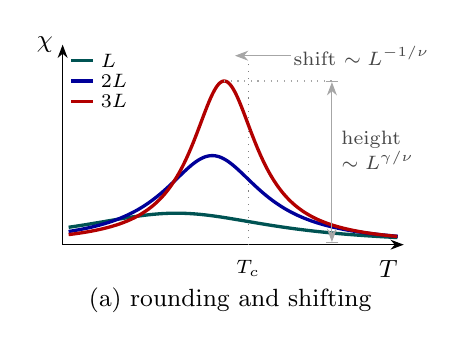
\begin{tikzpicture}[>=Stealth,font=\small,x=1.52cm,y=0.40cm]
  \draw[->] (-1.55,0) -- (1.30,0);
  \node[anchor=north east,inner sep=2pt] at (1.30,-0.30) {$T$};
  \draw[->] (-1.55,0) -- (-1.55,6.35) node[left]{$\chi$};
  \draw[dotted,gray] (0,0) -- (0,5.90);
  \node[anchor=north,font=\scriptsize] at (0,-0.20) {$T_c$};
  \draw[very thick,teal!65!black,domain=-1.5:1.25,samples=200,smooth,variable=\x]
       plot ({\x},{1/(1+(\x+0.60)*(\x+0.60))});
  \draw[very thick,blue!60!black,domain=-1.5:1.25,samples=240,smooth,variable=\x]
       plot ({\x},{2.828/(1+4*(\x+0.30)*(\x+0.30))});
  \draw[very thick,red!70!black,domain=-1.5:1.25,samples=300,smooth,variable=\x]
       plot ({\x},{5.196/(1+9*(\x+0.20)*(\x+0.20))});
  \draw[very thick,teal!65!black] (-1.48,5.85) -- (-1.30,5.85);
  \node[anchor=west,font=\scriptsize,inner sep=1.5pt] at (-1.27,5.85) {$L$};
  \draw[very thick,blue!60!black] (-1.48,5.20) -- (-1.30,5.20);
  \node[anchor=west,font=\scriptsize,inner sep=1.5pt] at (-1.27,5.20) {$2L$};
  \draw[very thick,red!70!black] (-1.48,4.55) -- (-1.30,4.55);
  \node[anchor=west,font=\scriptsize,inner sep=1.5pt] at (-1.27,4.55) {$3L$};
  \draw[<-,thin,gray!70] (-0.11,6.00) -- (0.36,6.00);
  \node[anchor=west,font=\scriptsize,gray!55!black,inner sep=1.5pt] at (0.34,6.00)
       {shift $\sim L^{-1/\nu}$};
  \draw[dotted,gray!70] (-0.20,5.196) -- (0.70,5.196);
  \draw[|<->|,thin,gray!70] (0.70,0.05) -- (0.70,5.196);
  \node[anchor=west,font=\scriptsize,gray!55!black,align=left,inner sep=1.5pt]
       at (0.74,3.00) {height\\ $\sim L^{\gamma/\nu}$};
  \node[anchor=north,font=\small] at (-0.15,-1.05) {(a) rounding and shifting};
\end{tikzpicture}
\hfill
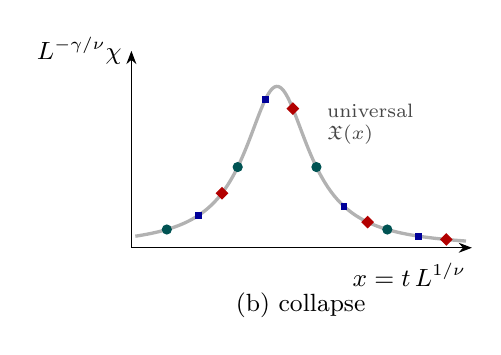
\begin{tikzpicture}[>=Stealth,font=\small,x=0.50cm,y=2.05cm]
  \draw[->] (-4.30,0) -- (4.35,0);
  \node[anchor=north east,inner sep=2pt] at (4.35,-0.06) {$x=t\,L^{1/\nu}$};
  \draw[->] (-4.30,0) -- (-4.30,1.22) node[left]{$L^{-\gamma/\nu}\chi$};
  \draw[very thick,gray!60,domain=-4.2:4.2,samples=200,smooth,variable=\x]
       plot ({\x},{1/(1+(\x+0.60)*(\x+0.60))});
  \foreach \x in {-3.4,-1.6,0.4,2.2}
     \node[circle,draw=teal!65!black,fill=teal!65!black,inner sep=1.15pt]
        at (\x,{1/(1+(\x+0.60)*(\x+0.60))}) {};
  \foreach \x in {-2.6,-0.9,1.1,3.0}
     \node[rectangle,draw=blue!60!black,fill=blue!60!black,inner sep=1.05pt]
        at (\x,{1/(1+(\x+0.60)*(\x+0.60))}) {};
  \foreach \x in {-2.0,-0.2,1.7,3.7}
     \node[diamond,draw=red!70!black,fill=red!70!black,inner sep=1.05pt]
        at (\x,{1/(1+(\x+0.60)*(\x+0.60))}) {};
  \node[anchor=north west,font=\scriptsize,gray!55!black,align=left,inner sep=1.5pt]
       at (0.55,0.92) {universal\\ $\mathfrak{X}(x)$};
  \node[anchor=north,font=\small] at (0,-0.22) {(b) collapse};
\end{tikzpicture}

\vspace{2ex}
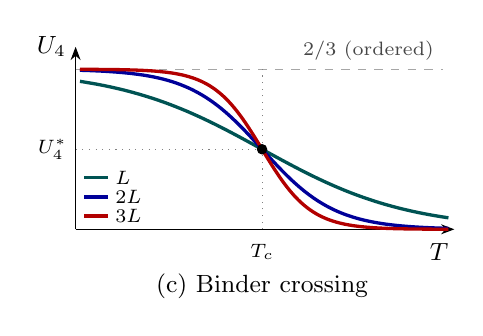
\begin{tikzpicture}[>=Stealth,font=\small,x=1.85cm,y=3.05cm]
  \draw[->] (-1.28,0) -- (1.32,0);
  \node[anchor=north east,inner sep=2pt] at (1.32,-0.035) {$T$};
  \draw[->] (-1.28,0) -- (-1.28,0.76) node[left]{$U_4$};
  \draw[dashed,gray!70] (-1.28,0.6667) -- (1.24,0.6667);
  \node[anchor=south east,font=\scriptsize,gray!55!black,inner sep=2pt]
       at (1.22,0.6800) {$2/3$ (ordered)};
  \draw[dotted,gray] (0,0) -- (0,0.6667);
  \draw[dotted,gray] (-1.28,0.3333) -- (0,0.3333);
  \node[anchor=north,font=\scriptsize] at (0,-0.020) {$T_c$};
  \node[anchor=east,font=\scriptsize,inner sep=2pt] at (-1.30,0.3333) {$U_4^{\ast}$};
  \draw[very thick,teal!65!black,domain=-1.25:1.28,samples=200,smooth,variable=\x]
       plot ({\x},{0.6667/(1+exp(2*\x))});
  \draw[very thick,blue!60!black,domain=-1.25:1.28,samples=200,smooth,variable=\x]
       plot ({\x},{0.6667/(1+exp(4*\x))});
  \draw[very thick,red!70!black,domain=-1.25:1.28,samples=200,smooth,variable=\x]
       plot ({\x},{0.6667/(1+exp(6*\x))});
  \fill (0,0.3333) circle (1.9pt);
  \draw[very thick,teal!65!black] (-1.22,0.215) -- (-1.06,0.215);
  \node[anchor=west,font=\scriptsize,inner sep=1.5pt] at (-1.04,0.215) {$L$};
  \draw[very thick,blue!60!black] (-1.22,0.135) -- (-1.06,0.135);
  \node[anchor=west,font=\scriptsize,inner sep=1.5pt] at (-1.04,0.135) {$2L$};
  \draw[very thick,red!70!black] (-1.22,0.055) -- (-1.06,0.055);
  \node[anchor=west,font=\scriptsize,inner sep=1.5pt] at (-1.04,0.055) {$3L$};
  \node[anchor=north,font=\small] at (0,-0.145) {(c) Binder crossing};
\end{tikzpicture}
\caption{The three faces of equation (FSS). \textbf{(a)} A finite system has no
divergence: $\chi(T,L)$ is a smooth peak that is \emph{rounded} over a width
$\sim L^{-1/\nu}$, \emph{shifted} from $T_c$ by the same order, and whose height
grows as $L^{\gamma/\nu}$. Both the height and the shift are exponent
measurements; the height needs no knowledge of $T_c$. \textbf{(b)} The same data
plotted as $L^{-\gamma/\nu}\chi$ against $x=tL^{1/\nu}$ collapse onto the single
universal function $\mathfrak{X}$ --- an excellent diagnostic, a poor estimator.
\textbf{(c)} The Binder cumulant is dimensionless, so no power of $L$ multiplies
its scaling function: $U_4=\mathfrak{U}(tL^{1/\nu})$. Hence all curves pass
through the same point at $t=0$, locating $T_c$ and the universal value
$U_4^{\ast}$ without any fit, while the slope at the crossing grows as
$L^{1/\nu}$. Exponents are illustrative, chosen for legibility rather than taken
from a real universality class.}
\label{fig:fss}
\end{figure}

\subsection{Corrections to scaling, and why they set the accuracy}
\label{sec:fss:corrections}

Restoring the leading irrelevant field $u$ of (S5) --- which enters (FSS) as a
third argument scaling as $uL^{-\omega}$ --- and expanding, every observable takes
the form
\[
\boxed{\;
A(t{=}0,L)=a_0\,L^{\rho}\Big(1+a_1L^{-\omega}+a_2L^{-2\omega}
+a_3L^{-1/\nu}+\dots\Big)+a_{\rm reg}
\;}
\]
The four kinds of term have four different origins: $a_1L^{-\omega}$ from the
irrelevant operator; $a_2L^{-2\omega}$ from its second order; $a_3L^{-1/\nu}$
from the nonlinearity of the scaling fields; and $a_{\rm reg}$ from the analytic
background. Three practical consequences follow, and together they account for
most of the difference between a $1\%$ and a $0.01\%$ exponent determination.

\paragraph{Effective exponents drift, and the drift is the systematic error.}
Fitting the pure power $A=a_0L^{\rho}$ to data over a window $[L_{\min},L_{\max}]$
returns not $\rho$ but
\[
\rho_{\rm eff}(L)=\frac{d\ln A}{d\ln L}
=\rho-a_1\omega L^{-\omega}+\dots ,
\]
which approaches $\rho$ only as fast as $L^{-\omega}$. With $\omega\simeq0.83$,
doubling $L$ reduces the bias by only a factor $\approx1.8$. This is why
increasing statistics at fixed $L$ eventually stops helping: the error becomes
entirely systematic, and the only cures are larger $L$, fitting the corrections
explicitly, or choosing observables whose $a_1$ happens to be small.

\paragraph{Dimensionless ratios are preferable, and improved observables better
still.} Quantities such as $U_4$ and $\xi_L/L$ carry $\rho=0$ and no
non-universal amplitude, which removes two fit parameters and typically reduces
$|a_1|$ as well. Better yet, if two observables have corrections of the same
form, a linear combination can be constructed with $a_1=0$; and in some models a
parameter of the Hamiltonian can be tuned so that the amplitude of the leading
irrelevant operator vanishes outright (``improved actions'', e.g.\ the
$\phi^{4}$ lattice model at $\lambda\simeq1.1$ in $d=3$, or the Blume--Capel model
at its optimal crystal field). Improved models are how the highest-precision
Monte Carlo exponents are obtained: with $a_1\approx0$ the leading correction
becomes $L^{-2\omega}$, and the systematic error falls by more than an order of
magnitude at the same $L$.

\paragraph{Do not measure $\alpha$ directly.} Collecting the earlier remarks: for
the three-dimensional Ising class $\alpha\simeq0.11$, so
$c_{\max}\sim L^{0.175}$ --- a factor $2$ over a decade in $L$ --- sitting on top
of an $L$-independent background $c_{\rm reg}$ of comparable or larger size, plus
corrections. Fitting three parameters ($c_{\rm reg}$, $a_0$, $\alpha/\nu$) to such
data is ill-conditioned, and the fitted exponent is strongly correlated with the
fitted background. The correct procedure is to measure $\nu$ well --- from
$L^{1/\nu}$-scaling quantities, which are clean --- and then use hyperscaling,
\[
\alpha=2-d\nu .
\]
With $\nu=0.62997(1)$ in $d=3$ this gives $\alpha=0.11009(3)$, far better than any
direct fit to $c$. The same logic applies to $\eta$: obtain it from
$\gamma/\nu=2-\eta$ or from the correlation function, whichever is cleaner in the
model at hand, and cross-check.

\subsection{First-order transitions: the other finite-size scaling}
\label{sec:fss:firstorder}

At a first-order transition $\xi$ does not diverge, so (S1) fails and the whole
construction above is inapplicable. Something equally systematic replaces it, and
because the standard numerical task is to \emph{decide} whether a transition is
continuous or first order, the two sets of predictions are best derived and then
compared.

\paragraph{The two-state model.} Near $T_t$ the system is, to exponential
accuracy in $V$, a two-level system: it is either in the ordered phase (energy
density $e_o$) or the disordered one ($e_d$), with the interfacial configurations
exponentially suppressed as shown in Section~\ref{sec:firstorder}. So take
\[
P(E)=p\,\delta(E-Ve_o)+q\,\delta(E-Ve_d),\qquad q=1-p,
\qquad
\frac{p}{q}=e^{-\beta V\left[f_o(T)-f_d(T)\right]} .
\]
Since $f_o-f_d$ vanishes at $T_t$ with slope $-(s_o-s_d)=-\Delta s$, we have
$f_o-f_d\simeq-\Delta s\,(T-T_t)$, so
\[
\frac{p}{q}=\exp\!\left[\frac{V\,\Delta s\,(T-T_t)}{k_BT}\right] .
\]
Every first-order result follows from these two lines.

\paragraph{Width of the transition region, $\Delta T\sim L^{-d}$.} The weights
swing from $p\approx1$ to $p\approx0$ as the exponent passes through zero, i.e.\
over
\[
|T-T_t|\;\sim\;\frac{k_BT_t}{V\,\Delta s}\;\sim\;L^{-d} .
\]
So $L^{-d}$ replaces $L^{-1/\nu}$ as the rounding width, and the shift of any
pseudo-critical temperature from $T_t$ is of the same order.

\paragraph{Specific heat, $c_{\max}\sim L^{d}$.} With $\Delta e=e_o-e_d$,
\[
\Var(E)=pq\,V^{2}(\Delta e)^{2},
\qquad
c=\frac{\Var(E)}{Vk_BT^{2}}=\frac{pq\,V(\Delta e)^{2}}{k_BT^{2}} ,
\]
using the canonical result of Section~\ref{sec:canonical}. At $T_t$ the two
phases carry equal weight, $p=q=\tfrac12$, so
\[
\boxed{\;c_{\max}\simeq\frac{V(\Delta e)^{2}}{4k_BT_t^{2}}\;\sim\;L^{d}\;}
\]
The mechanism is transparent: a latent heat is a finite energy jump, and forcing
it into a temperature window of width $L^{-d}$ produces a specific heat of height
$L^{d}$. The area under the peak, $c_{\max}\Delta T$, is $L$-independent and equal
to the latent heat --- as it must be.

\paragraph{The energy cumulant, in closed form.} The Challa--Landau--Binder
cumulant $V_L=1-\langle E^{4}\rangle/3\langle E^{2}\rangle^{2}$ can be evaluated
exactly in the two-state model. Writing $X=Ve_o$, $Y=Ve_d$,
\[
\langle E^{2}\rangle=pX^{2}+qY^{2},
\qquad
\langle E^{4}\rangle=pX^{4}+qY^{4} .
\]
Extremising over $p$: setting $\partial_p\big[\langle E^{4}\rangle/\langle
E^{2}\rangle^{2}\big]=0$ gives
$(X^{2}+Y^{2})(pX^{2}+qY^{2})=2(pX^{4}+qY^{4})$, hence
$X^{2}Y^{2}=pX^{4}+qY^{4}$ and therefore
\[
p=\frac{Y^{2}}{X^{2}+Y^{2}},\qquad
\langle E^{2}\rangle=\frac{2X^{2}Y^{2}}{X^{2}+Y^{2}},\qquad
\langle E^{4}\rangle=X^{2}Y^{2} .
\]
Substituting,
\[
\boxed{\;
V_L^{\min}=1-\frac{(e_o^{2}+e_d^{2})^{2}}{12\,e_o^{2}e_d^{2}}
=\frac{2}{3}-\frac{1}{12}\left(\frac{e_o}{e_d}-\frac{e_d}{e_o}\right)^{2}
\;}
\]
(the factors of $V$ cancel identically). The two forms are equal because
$(r+r^{-1})^{2}=(r-r^{-1})^{2}+4$. The result is worth its space: it reproduces
$V_L^{\min}=2/3$ exactly when $e_o=e_d$, i.e.\ when there is no latent heat, which
is the continuous case; the deviation from $2/3$ is a direct, $L$-independent
measure of the latent heat; and it is a genuine prediction that can be checked
against the independently measured $e_o$ and $e_d$.

\paragraph{The magnetisation cumulant, $U_4^{\min}\sim-L^{d}$.} At a
symmetry-breaking first-order transition $P(m)$ has a peak at $m=0$ of Gaussian
width $\sigma_0^{2}=k_BT\chi_d/V$ (from $\Var(m)=k_BT\chi/V$) coexisting with
peaks at $\pm m_s$. Keep the leading terms on the disordered side, with $w$ the
weight of the ordered peaks:
\[
\langle m^{2}\rangle\simeq\sigma_0^{2}+w\,m_s^{2},
\qquad
\langle m^{4}\rangle\simeq3\sigma_0^{4}+w\,m_s^{4} .
\]
Introduce $\varepsilon=w\,m_s^{2}/\sigma_0^{2}$ and $\kappa=m_s^{2}/\sigma_0^{2}$,
so that
\[
\frac{\langle m^{4}\rangle}{3\langle m^{2}\rangle^{2}}
=\frac{3+\varepsilon\kappa}{3(1+\varepsilon)^{2}} .
\]
Maximising over $\varepsilon$ (i.e.\ scanning $T$ through the transition) gives
$\varepsilon=(\kappa-6)/\kappa\to1$ for large $\kappa$, whence
\[
U_4^{\min}\simeq1-\frac{\kappa}{12}
=1-\frac{m_s^{2}\,V}{12\,k_BT_t\,\chi_d}\;\sim\;-L^{d} .
\]
So the Binder cumulant, which is bounded and $L$-independent at a continuous
transition, plunges to large negative values proportional to the volume at a
first-order one. That contrast --- not the value of any exponent --- is the
standard diagnostic.

\paragraph{First-order transitions as a formal exponent set.} The two columns
unify neatly. Setting
\[
\nu=\frac{1}{d},\qquad \alpha=1,\qquad \beta=0,\qquad \gamma=1,
\qquad \eta=2-d,
\]
one has $L^{-1/\nu}=L^{-d}$, $L^{\alpha/\nu}=L^{d}$, $L^{\gamma/\nu}=L^{d}$, and
$L^{-\beta/\nu}=L^{0}$ --- exactly the first-order results derived above. These
values satisfy both Rushbrooke, $\alpha+2\beta+\gamma=1+0+1=2$, and hyperscaling,
$2-\alpha=1=d\cdot\tfrac1d=d\nu$, as well as Fisher's
$\gamma/\nu=d=2-\eta$. The consistency is not a coincidence: a first-order
transition is the limiting case in which the correlation volume is replaced by the
system volume, and the scaling relations are insensitive to which of the two plays
that role.

\paragraph{The discriminant table.} Collecting everything, this is what one
actually looks at to decide the order of a transition:
\begin{center}
\renewcommand{\arraystretch}{1.2}
\begin{tabular}{lll}
\toprule
Quantity & Continuous & First order\\
\midrule
$c_{\max}$ (per site) & $L^{\alpha/\nu}$, or $\ln L$ if $\alpha=0$ & $L^{d}$\\
$\chi_{\max}$ & $L^{\gamma/\nu}$ & $L^{d}$\\
Peak width in $T$ & $L^{-1/\nu}$ & $L^{-d}$\\
$T_{\max}(L)-T_c$ & $L^{-1/\nu}$ & $L^{-d}$\\
$\langle|m|\rangle$ at the peak & $L^{-\beta/\nu}\to0$ & $O(1)$, nonzero\\
$U_4$ at the crossing & universal, $L$-independent & $U_4^{\min}\sim-L^{d}$\\
$V_L^{\min}$ (energy cumulant) & $2/3+O\!\big(L^{\alpha/\nu-d}\big)\to2/3$ &
  $\tfrac{2}{3}-\tfrac{1}{12}\big(\tfrac{e_o}{e_d}-\tfrac{e_d}{e_o}\big)^{2}$\\
$\ln\!\big(P_{\max}/P_{\min}\big)$ for $P(E)$ & $O(1)$, no growth & $2\sigma L^{d-1}$\\
\bottomrule
\end{tabular}
\end{center}
The last row is the Lee--Kosterlitz criterion of Section~\ref{sec:firstorder}, and
it is the most reliable of the set, because a barrier that \emph{grows} with $L$
cannot be mimicked by a continuous transition with unlucky corrections, whereas
$L^{d}$ and $L^{\gamma/\nu}$ can look similar over a limited range of $L$ when
$\gamma/\nu$ happens to be close to $d$. A weak first-order transition ---
$\xi$ large but finite --- looks continuous for all $L\lesssim\xi$ and reveals
itself only beyond; this is the standard difficulty with, for instance, the
three-state Potts model in three dimensions, and there is no cure but larger $L$.

\subsection{A conventional high-accuracy implementation}
\label{sec:fss:implementation}

What follows is the standard modern protocol, in the order one executes it. It is
deliberately conventional: every ingredient is textbook, and the accuracy comes
from the combination and from the systematic-error control, not from novelty.

\paragraph{Step 1: geometry and the size ladder.} Use $L^{d}$ sites with periodic
boundaries in every direction, aspect ratio fixed at $1{:}1{:}\dots{:}1$, and a
roughly \emph{geometric} sequence of sizes,
\[
L\in\{8,\;12,\;16,\;24,\;32,\;48,\;64,\;96,\;128,\dots\},
\]
spanning at least one and preferably one and a half decades. Geometric spacing
matters for two reasons: fits are performed in $\ln L$, where geometric spacing
distributes leverage evenly; and the pairs $(L,2L)$ needed for the quotient method
of Step 6 exist by construction. Choose the ratio $s=2$ (or $s=3/2$ for a denser
ladder) and keep it fixed.

\paragraph{Step 2: algorithm --- defeat critical slowing down first.} At $T_c$ the
relaxation time of a local update diverges as $\tau\sim L^{z}$ with $z\approx2$
for Metropolis or heat-bath dynamics ($z$ here is the dynamic critical exponent,
not the fugacity of Section~\ref{sec:ensembles}). Since one sweep costs $L^{d}$
operations, the cost of one \emph{independent} configuration is $L^{d+z}\approx
L^{5}$ in $d=3$: increasing $L$ from $32$ to $128$ then costs a factor $10^{3}$.
This, and not the physics, is what limits accessible $L$, so the algorithm choice
dominates everything else.
\begin{itemize}
\item \emph{Ferromagnetic Ising, Potts, $O(n)$}: use a cluster algorithm ---
Swendsen--Wang or Wolff. These reduce the dynamic exponent to
$z_{\rm cl}\approx0.3$--$0.5$, essentially eliminating critical slowing down, and
they are the reason that high-precision three-dimensional exponents exist at all.
\item \emph{Loop, dimer, and worldline models}: worm/directed-loop algorithms.
\item \emph{Frustrated or disordered models}, where no cluster algorithm exists:
parallel tempering (replica exchange) over a temperature ladder, which also
supplies several temperatures at once for Step 5.
\item \emph{First-order transitions}: local and cluster algorithms both fail,
because the tunnelling time between the two peaks of $P(E)$ grows as
$e^{2\sigma L^{d-1}/k_BT}$ (Section~\ref{sec:firstorder}). Use multicanonical
sampling or Wang--Landau, which flatten $P(E)$ by construction and reduce the
tunnelling time to a power of $L$.
\end{itemize}

\paragraph{Step 3: equilibration, tested and not assumed.} Discard $n_{\rm
eq}\gtrsim20\,\tau_{\rm exp}$ initial sweeps, where $\tau_{\rm exp}$ is the
\emph{exponential} (slowest-mode) autocorrelation time, which can exceed the
integrated time of Step 4. Two cheap and decisive tests:
\begin{itemize}
\item \emph{Two-sided approach.} Start one run from a fully ordered configuration
and another from a random one, and require that the two converge to the same
value from opposite sides. This catches incomplete equilibration that a single
run hides, and it is mandatory near a first-order transition, where the two runs
can remain trapped in different phases indefinitely --- itself a useful signal.
\item \emph{Doubling test.} Recompute the estimate using only the second half of
the data. If it moves by more than its error bar, the run is not equilibrated.
\end{itemize}

\paragraph{Step 4: observables and honest error bars.} Store, per measurement, the
raw quantities and not their combinations:
\[
E,\quad m,\quad m^{2},\quad m^{4},\quad |m|,\quad m^{2}E,\quad |m|E,\quad
\widetilde{G}(0),\quad \widetilde{G}(k_1) ,
\]
where $\widetilde{G}(k)=V^{-1}\big|\sum_{\mathbf{x}}s_{\mathbf{x}}
e^{i\mathbf{k}\cdot\mathbf{x}}\big|^{2}$ and $k_1=2\pi/L$ is the smallest nonzero
momentum. Then
\[
\chi=\frac{V\langle m^{2}\rangle}{k_BT},
\qquad
c=\frac{\Var(E)}{Vk_BT^{2}},
\qquad
U_4=1-\frac{\langle m^{4}\rangle}{3\langle m^{2}\rangle^{2}},
\]
and the \emph{second-moment correlation length}, which is the standard
high-accuracy definition because it requires only two Fourier modes,
\[
\boxed{\;
\xi_L=\frac{1}{2\sin(\pi/L)}
\sqrt{\frac{\widetilde{G}(0)}{\widetilde{G}(k_1)}-1}\;}
\]
(one checks that for a free propagator $\widetilde G(k)^{-1}\propto
\hat k^{2}+\xi^{-2}$ this returns $\xi$ exactly, with $\hat
k=2\sin(k/2)$ the lattice momentum; note $\widetilde G(0)=V\langle m^{2}\rangle$,
so $\chi$ and $\xi_L$ come from the same measurement).

Error bars require two ingredients, both mandatory:
\begin{itemize}
\item \emph{Integrated autocorrelation time with automatic windowing.} With
$\rho(k)=C(k)/C(0)$ the normalised autocorrelation function of the measured
series,
\[
\tau_{\rm int}(W)=\frac12+\sum_{k=1}^{W}\rho(k),
\qquad
\sigma^{2}(\bar A)=\frac{2\tau_{\rm int}\,C(0)}{N} ,
\]
with $W$ chosen self-consistently as the smallest $W$ satisfying
$W\geq c\,\tau_{\rm int}(W)$, $c\approx6$--$10$ (the Madras--Sokal window). The
factor $2\tau_{\rm int}$ is the whole point: omitting it underestimates the error
by an order of magnitude at large $L$, which then makes fits look artificially
good and biases exponents without warning.
\item \emph{Jackknife for anything nonlinear.} $U_4$, $\xi_L/L$, $c$, and
$\partial\ln\langle m^{2}\rangle/\partial\beta$ are all \emph{nonlinear functions
of correlated averages}, for which naive error propagation is wrong. Partition the
series into $B$ blocks each of length $\gg\tau_{\rm int}$, form the delete-one
estimates $\hat\theta_{(b)}$ from all data except block $b$, and use
\[
\sigma^{2}_{\rm jack}(\hat\theta)=\frac{B-1}{B}\sum_{b=1}^{B}
\big(\hat\theta_{(b)}-\bar{\hat\theta}\big)^{2} .
\]
This handles bias and correlation together and is the standard choice.
\end{itemize}

\paragraph{Step 5: reweighting, to obtain continuous temperature dependence.}
Peak locations and crossing points must be found to a precision far finer than any
practical grid of simulation temperatures. The solution is
multiple-histogram (Ferrenberg--Swendsen) reweighting: from runs at
$\beta_1,\dots,\beta_R$ with $N_r$ measurements each, the estimator at
\emph{any} $\beta$ is
\[
\boxed{\;
\langle A\rangle_{\beta}=
\frac{\displaystyle\sum_{r=1}^{R}\sum_{j=1}^{N_r} A_{rj}\,
\frac{e^{-\beta E_{rj}}}{\sum_{s}(N_s/Z_s)\,e^{-\beta_s E_{rj}}}}
{\displaystyle\sum_{r=1}^{R}\sum_{j=1}^{N_r}
\frac{e^{-\beta E_{rj}}}{\sum_{s}(N_s/Z_s)\,e^{-\beta_s E_{rj}}}}\;}
\]
where the partition functions are fixed self-consistently by iterating
\[
Z_s=\sum_{r}\sum_{j}
\frac{e^{-\beta_s E_{rj}}}{\sum_{s'}(N_{s'}/Z_{s'})\,e^{-\beta_{s'}E_{rj}}} ,
\]
to convergence (only ratios of the $Z_s$ are determined, as they must be: the
overall normalisation is free). Practical notes: work with $\ln Z_s$ and a
log-sum-exp evaluation to avoid overflow; space the $\beta_r$ so that neighbouring
energy histograms overlap substantially, which for a critical system means
$\Delta\beta\sim L^{-1/\nu}$ and for a first-order one $\Delta\beta\sim L^{-d}$;
and propagate errors through the reweighting by jackknifing over whole blocks of
the original series, never by reweighting the error bars.

Reweighting also removes the need for numerical differentiation: as noted in
Section~\ref{sec:fss:observables}, $\partial_\beta\langle
A\rangle=\langle A\rangle\langle E\rangle-\langle AE\rangle$ gives every
temperature derivative exactly from measured correlators.

\paragraph{Step 6: the estimator hierarchy --- prefer the quotient method.} Now
extract exponents. Ordered from most to least robust:

\emph{(a) The quotient (phenomenological renormalisation) method.} Take any
dimensionless $R$ with $R(t,L)=\mathfrak{r}(tL^{1/\nu})+L^{-\omega}\mathfrak{r}_1(tL^{1/\nu})$
--- use $\xi_L/L$ and $U_4$. For each pair $(L,sL)$, find the crossing
temperature $\beta_{\rm cross}(L)$ where $R(L)=R(sL)$. Linearising about $t=0$
with $u=tL^{1/\nu}$,
\[
\mathfrak{r}'(0)\,u\big(1-s^{1/\nu}\big)
=L^{-\omega}\mathfrak{r}_1(0)\big(s^{-\omega}-1\big)
\quad\Longrightarrow\quad
t_{\rm cross}\;\propto\;L^{-\omega-1/\nu} ,
\]
so the crossing converges to $T_c$ much faster than any peak position does
($L^{-\omega-1/\nu}$ against $L^{-1/\nu}$). Then, for any observable
$A=L^{\rho}\mathfrak{a}(x)(1+\dots)$, evaluate the \emph{quotient at the crossing}:
\[
\boxed{\;
Q_A\equiv\frac{A(\beta_{\rm cross},sL)}{A(\beta_{\rm cross},L)}
=s^{\rho}\Big[1+O(L^{-\omega})\Big]
\quad\Longrightarrow\quad
\rho=\frac{\ln Q_A}{\ln s}\;}
\]
because $x\to0$ at the crossing. With $A=\chi$ this gives $\gamma/\nu$; with
$A=\partial_\beta R$, which scales as $L^{1/\nu}$, it gives $\nu$; with
$A=\langle|m|\rangle$ it gives $\beta/\nu$. The virtues are that $T_c$ never has
to be known, that each exponent comes from a two-point ratio rather than a global
fit, and that the residual corrections are a single clean $L^{-\omega}$ which can
be fitted and extrapolated. This is how the best Monte Carlo exponents are
obtained.

\emph{(b) Peak scaling.} $\chi_{\max}\sim L^{\gamma/\nu}$ and
$[\partial U_4/\partial T]_{\max}\sim L^{1/\nu}$, also $T_c$-free but with slower
convergence, since the peak sits at $x=x_{\max}\neq0$ where the correction
amplitudes are larger.

\emph{(c) Fits at a fitted $T_c$.} Simultaneously fit $T_c$ and the exponents to
data over a window in $t$ and $L$. Correct in principle, but $T_c$ and the
exponents are strongly correlated, and an error in $T_c$ masquerades as a shift in
$\nu$.

\emph{(d) Data collapse.} Diagnostic only, as argued above.

\paragraph{Step 7: systematic-error control --- the $L_{\min}$ scan.} This step,
not the statistics, determines the quoted accuracy. Fit the correction-including
form
\[
A(L)=a_0L^{\rho}\big(1+a_1L^{-\omega}\big)
\]
repeatedly, each time discarding all data with $L<L_{\min}$, and tabulate the
fitted $\rho$ and the goodness of fit $\chi^{2}/\mathrm{dof}$ against
$L_{\min}$. Three things to require:
\begin{itemize}
\item $\chi^{2}/\mathrm{dof}\approx1$ with an acceptable $p$-value. A value $\gg1$
means unmodelled corrections; $\ll1$ usually means overestimated error bars.
\item A \emph{plateau}: the fitted $\rho$ must stop drifting as $L_{\min}$
increases, within errors. If it is still drifting at the largest usable
$L_{\min}$, the corrections are not under control and no exponent should be
quoted.
\item The quoted uncertainty must be the \emph{quadrature sum} of the statistical
error from the plateau fits and a systematic contribution taken from the residual
drift across the plateau. Reporting only the statistical error of one fit is the
commonest way that published exponents disagree by many standard deviations.
\end{itemize}
Fit $\omega$ if the data support it; otherwise fix it to a literature value and
repeat the analysis with $\omega$ varied over its uncertainty, adding the induced
spread to the systematic error. Repeat the whole analysis with a second
observable (e.g.\ $U_4$ instead of $\xi_L/L$): agreement between two independent
routes is the strongest available evidence that the systematic error has been
correctly estimated.

\paragraph{Step 8: validation against known answers.} Before trusting a new
measurement, reproduce a known one with the same code and the same analysis
pipeline.
\begin{itemize}
\item \emph{Two-dimensional Ising}, where everything is exact:
$k_BT_c/J=2/\ln(1+\sqrt2)=2.269185\ldots$, $\nu=1$, $\beta=1/8$, $\gamma=7/4$,
$\eta=1/4$, $\alpha=0$ (logarithmic). Any pipeline that cannot recover
$\gamma/\nu=7/4$ to three digits is not ready for a harder problem.
\item \emph{Three-dimensional Ising}, where conformal-bootstrap values are far
more accurate than Monte Carlo: $\nu=0.629971(4)$, $\eta=0.036298(2)$,
$\omega=0.8295(6)$, giving $1/\nu=1.58738$, $\gamma/\nu=2-\eta=1.96370$,
$\beta/\nu=(1+\eta)/2=0.51815$, and $\alpha=2-3\nu=0.110087$.
\item \emph{Universal amplitude ratios} as an independent check that the
\emph{scaling functions}, not merely the exponents, are right: for the
three-dimensional Ising class in a periodic cube, $U_4^{\ast}\approx0.465$
(equivalently $\langle m^{2}\rangle^{2}/\langle m^{4}\rangle\approx0.623$) and
$\xi_L/L\big|_{T_c}\approx0.64$. Both are convention- and
boundary-condition-dependent, so compare only against a value computed with
\emph{the same} definitions and geometry.
\end{itemize}

\paragraph{Step 9: a cost budget.} With a cluster algorithm the cost of one
independent measurement is $\sim L^{d+z_{\rm cl}}$, so at fixed CPU the number of
independent samples falls as $L^{-(d+z_{\rm cl})}$. Two rules of thumb follow.
First, allocate CPU so that the \emph{relative} statistical error of the fitted
quantity is comparable across $L$ --- which means spending most of the budget on
the largest two or three sizes, since a least-squares fit is limited by its worst
points and the large-$L$ points carry the least systematic contamination. Second,
prefer a longer ladder of $L$ over one heroic size: the $L_{\min}$ scan of Step 7
has no power without several sizes above $L_{\min}$, and a single very large $L$
cannot demonstrate that corrections have died away.

\paragraph{Step 10: the pitfall checklist.} Each of these has produced published
errors:
\begin{enumerate}
\item Omitting the factor $2\tau_{\rm int}$, hence error bars too small by
$\sqrt{2\tau_{\rm int}}$ and a spuriously good $\chi^{2}$.
\item Propagating errors analytically through $U_4$ or $\xi_L/L$ instead of
jackknifing.
\item Mixing $\langle|m|\rangle$ with $\langle m^{2}\rangle^{1/2}$, or $\chi$ with
$\chi'$, within one fit.
\item Fitting $c$ to extract $\alpha$ instead of using $\alpha=2-d\nu$.
\item Treating the $\chi$-peak and $c$-peak temperatures as the same
pseudo-critical point.
\item Changing the aspect ratio or boundary conditions between sizes.
\item A poor random number generator. Cluster algorithms are notoriously
sensitive to subtle generator correlations, which produce systematic errors far
exceeding the statistical ones while leaving all consistency checks intact; use a
well-tested generator with a long period and verify against the exact
two-dimensional results.
\item Quoting only statistical errors, with no $L_{\min}$ scan.
\item At a suspected first-order transition, not checking for barrier crossing:
a run that never tunnels reports a perfectly smooth unimodal $P(E)$ and looks
continuous.
\item Assuming self-averaging in a disordered system. There, sample-to-sample
fluctuations of $\chi$ do \emph{not} vanish relative to the mean, so the number
of disorder realisations --- not the length of each run --- controls the error,
and the two averages must be nested correctly.
\end{enumerate}

\subsection{Where the assumptions fail}
\label{sec:fss:failures}

Finally, the boundaries of the method, following the numbering of
Section~\ref{sec:fss:assumptions}.

\begin{itemize}
\item \textbf{Above the upper critical dimension} ($d>4$ for Ising-like systems)
hyperscaling fails, so (S2) fails and with it the $L^{-d}$ prefactor of (FSS).
The mechanism is a \emph{dangerous irrelevant variable}: the quartic coupling has
eigenvalue $y_u=4-d<0$, so it is irrelevant, but the scaling function is singular
in it, and the limit $u L^{-\omega}\to0$ cannot be taken naively. Finite-size
scaling above $d_c$ is well understood but has a modified form; standard (FSS) is
simply wrong there. Exactly at $d=d_c$ one gets multiplicative logarithmic
corrections, which must be included or the exponents come out biased.
\item \textbf{Kosterlitz--Thouless transitions.} Here $\xi$ diverges
\emph{exponentially}, $\xi\sim\exp\big(b/\sqrt{t}\big)$, so $\nu$ is formally
infinite and $L^{1/\nu}$ degenerates. The scaling variable becomes $\ln L$, and
there are multiplicative logarithmic corrections; the two-dimensional XY model
requires this modified treatment, and applying standard (FSS) to it yields
meaningless drifting exponents.
\item \textbf{Long-range interactions.} A pair potential $\sim r^{-\sigma}$ with
$\sigma\leq d$ destroys extensivity outright (the warning in
Section~\ref{sec:criticalnonanalytic}); for $d<\sigma<d+2-\eta_{\rm sr}$ the
transition is controlled by a distinct fixed point with its own exponents, and
periodic boundaries must be implemented with care since the interaction wraps the
box.
\item \textbf{Quenched disorder.} Two amendments. Self-averaging fails for the
singular parts, so $\Var_{\rm samples}(\chi)/\langle\chi\rangle^{2}$ tends to a
nonzero constant, and the disorder average is the expensive part of the
calculation. And if the disorder couples to the energy density, the specific-heat
exponent of the pure system controls whether disorder is relevant at all
(Harris criterion: relevant if $\alpha>0$, i.e.\ $d\nu<2$).
\item \textbf{Weak first-order transitions.} Section~\ref{sec:fss:firstorder}
applies only for $L\gg\xi$; for $L\lesssim\xi$ the transition mimics a continuous
one perfectly, and no analysis of data with $L\lesssim\xi$ can tell the
difference. The honest conclusion in such a case is that the order of the
transition is undetermined at the sizes studied.
\item \textbf{Free or otherwise non-periodic boundaries.} (S4) is violated in the
specific sense that the free energy acquires a genuine surface term
$\propto L^{d-1}$, i.e.\ a correction of relative order $L^{-1}$ that adds to the
$L^{-\omega}$ series and, since typically $\omega<1$, is subleading but not
negligible. Surface critical behaviour introduces its own exponents. Periodic
boundaries avoid all of this, which is why they are standard.
\end{itemize}

In every one of these cases the failure is traceable to a specific assumption of
Section~\ref{sec:fss:assumptions}, which is the practical reason for having
separated them: when finite-size scaling does not work, the diagnosis is a
question of identifying which of (S1)--(S5) has been violated.

\section{Volumetric heat capacity}

We use the volumetric (per unit volume) heat capacity
\[
\boxed{\;c_V=\frac{1}{V}\left(\frac{\dbar Q}{dT}\right)_V\;}
\]
with $\dbar Q_{\rm rev}=T\,dS$ from Section~\ref{sec:heat}, so that equivalently
and more safely
\[
c_V=\frac{T}{V}\left(\frac{\partial S}{\partial T}\right)_V .
\]
The second form is preferable as a \emph{definition}, since it refers only to
state functions and carries no hidden reversibility assumption. The subscript $V$
is not the whole story, however: one must also say what else is held fixed.

\subsection{Canonical ensemble: fixed \texorpdfstring{$N$}{N}}
\label{sec:canonical}

With $N$ fixed,
\[
c_V=\frac{T}{V}\left(\frac{\partial S}{\partial T}\right)_{V,N},
\]
and using $S=-(\partial F/\partial T)_{V,N}$,
\[
\boxed{\;c_V=-\frac{T}{V}\left(\frac{\partial^2F}{\partial T^2}\right)_{V,N}\;}
\]
Now insert $F=-k_BT\ln Z$ and change variables to $\beta$. Using
$d\beta/dT=-k_B\beta^{2}$ and $U=-\partial\ln Z/\partial\beta$,
\[
\boxed{\;c_V=\frac{k_B\beta^{2}}{V}
\left(\frac{\partial^{2}\ln Z}{\partial\beta^{2}}\right)_{V,N}\;}
\]
Since $\partial\ln Z/\partial\beta=-\langle E\rangle$ and
$\partial^{2}\ln Z/\partial\beta^{2}=\langle E^{2}\rangle-\langle E\rangle^{2}$,
\[
\boxed{\;c_V=\frac{\langle E^{2}\rangle-\langle E\rangle^{2}}{Vk_BT^{2}}
=\frac{\Var(E)}{Vk_BT^{2}}\;}
\]
The heat capacity is the energy variance: a system that absorbs a lot of heat per
kelvin is one whose energy fluctuates a lot at fixed temperature. Positivity of
$c_V$ is automatic.

\subsection{Grand canonical ensemble: fixed \texorpdfstring{$\mu$}{mu}}

Here $N$ fluctuates while $T,V,\mu$ are fixed. At constant volume,
$dU=T\,dS+\mu\,dN$, so that $d(U-\mu N)=T\,dS$ at fixed $\mu$, and the heat
absorbed is
\[
\boxed{\;\dbar Q_{\rm rev}=dU-\mu\,dN\;}
\]
i.e.\ the energy change minus the part carried in by the incoming particles.
Consequently
\[
\boxed{\;c_V=\frac{1}{V}\left(\frac{\partial (U-\mu N)}{\partial T}\right)_{V,\mu}
=\frac{T}{V}\left(\frac{\partial S}{\partial T}\right)_{V,\mu}\;}
\]

\begin{warning}
Splitting the energy flux of an open system into ``heat'' and ``matter
transport'' is a matter of convention, because particles entering the system
carry entropy as well as energy. The expression above should be read as the
definition $\dbar Q\equiv T\,dS$ at fixed $\mu$, which is self-consistent and is
the standard choice; other conventions (e.g.\ using the enthalpy per particle
rather than $\mu$) appear in the non-equilibrium and thermoelectric literature.
\end{warning}

Since $S=-(\partial\Omega/\partial T)_{V,\mu}$,
\[
\boxed{\;c_V=-\frac{T}{V}\left(\frac{\partial^{2}\Omega}{\partial T^{2}}\right)_{V,\mu}\;}
\]
and with $\Omega=-k_BT\ln\Xi$, exactly as in the canonical case,
\[
\boxed{\;c_V=\frac{k_B\beta^{2}}{V}
\left(\frac{\partial^{2}\ln\Xi}{\partial\beta^{2}}\right)_{V,\mu}\;}
\]
Differentiating at fixed $\mu$ (\emph{not} at fixed $\beta\mu$ --- this is a
frequent slip),
\[
\frac{\partial\ln\Xi}{\partial\beta}\bigg|_{\mu}=-\langle E-\mu N\rangle,
\qquad
\frac{\partial^{2}\ln\Xi}{\partial\beta^{2}}\bigg|_{\mu}=\Var(E-\mu N),
\]
so
\[
\boxed{\;c_{V,\mu}=\frac{\Var(E-\mu N)}{Vk_BT^{2}}
=\frac{\Var(E)+\mu^{2}\Var(N)-2\mu\,\Cov(E,N)}{Vk_BT^{2}}\;}
\]

\subsection{Caution: \texorpdfstring{$c_{V,\mu}\neq c_{V,N}$}{cVmu is not cVN}}
\label{sec:caveat}

The two boxed results are \emph{not} two computations of the same quantity; see
Section~\ref{sec:respdiffer} for why this is consistent with ensemble
equivalence. Writing $S$ and $N$ as functions of $(T,V,\mu)$ and using the
Maxwell relation $(\partial S/\partial\mu)_{T,V}=(\partial N/\partial T)_{V,\mu}$
from $d\Omega=-S\,dT-P\,dV-N\,d\mu$,
\[
\boxed{\;C_{V,N}=C_{V,\mu}
-\;T\,\frac{\big[(\partial N/\partial T)_{V,\mu}\big]^{2}}
{(\partial N/\partial\mu)_{T,V}}\;}
\]
Because $(\partial N/\partial\mu)_{T,V}=\beta\Var(N)>0$, the correction is
strictly negative: $C_{V,N}\leq C_{V,\mu}$, as stability requires. In fluctuation
language, using $(\partial N/\partial T)_{V,\mu}=k_B\beta^{2}\Cov(N,E-\mu N)$,
the $\mu$-dependence cancels identically and one is left with
\[
\boxed{\;c_{V,N}=\frac{1}{Vk_BT^{2}}
\left[\Var(E)-\frac{\Cov(E,N)^{2}}{\Var(N)}\right]\;}
\]
This is the grand-canonical expression for the ordinary fixed-$N$ heat capacity:
the energy variance with the part of the energy fluctuation that is ``explained
by'' the particle-number fluctuation projected out --- a conditional variance.

\paragraph{Worked check: classical ideal gas.} With
$\Omega=-k_BT\,e^{\beta\mu}V/\lambda_T^{3}$ and $\lambda_T\propto T^{-1/2}$, one
finds, writing $x=\beta\mu$,
\[
C_{V,\mu}=Nk_B\left(\tfrac{15}{4}-3x+x^{2}\right),
\qquad
C_{V,N}=\tfrac{3}{2}Nk_B,
\qquad
C_{V,\mu}-C_{V,N}=Nk_B\left(x-\tfrac{3}{2}\right)^{2}\geq 0 .
\]
The naive grand-canonical answer is not $\tfrac32 Nk_B$, and is not even
$\mu$-independent; the correction term restores the familiar result exactly.
Equivalently, for a Poissonian $N$ with $\Var(N)=N$ and, conditionally on $N$,
$\langle E\rangle=\tfrac32Nk_BT$ and $\Var(E|N)=\tfrac32N(k_BT)^{2}$, the law of
total variance gives $\Var(E)=\tfrac32N(k_BT)^{2}+\tfrac94N(k_BT)^{2}$ and
$\Cov(E,N)=\tfrac32k_BT\,N$, whence
$\Var(E)-\Cov(E,N)^{2}/\Var(N)=\tfrac32N(k_BT)^{2}$ and
$c_{V,N}=\tfrac32Nk_B/V$ as it must be.

\section{Key comparison}

\paragraph{Canonical.}
\[
\boxed{\;N=\text{fixed},\qquad
c_V=-\frac{T}{V}\left(\frac{\partial^{2}F}{\partial T^{2}}\right)_{V,N}
=\frac{\Var(E)}{Vk_BT^{2}}\;}
\]

\paragraph{Grand canonical.}
\[
\boxed{\;\mu=\text{fixed},\qquad
c_V=-\frac{T}{V}\left(\frac{\partial^{2}\Omega}{\partial T^{2}}\right)_{V,\mu}
=\frac{\Var(E-\mu N)}{Vk_BT^{2}}\;}
\]

\paragraph{The organising principles.}
\[
\boxed{\;\text{The natural potential is fixed by the variables the environment
holds fixed.}\;}
\]
\[
\boxed{\;\text{Potential}=-k_BT\ln(\text{partition function});\quad
\text{2nd derivative}=\text{response}=\text{variance.}\;}
\]
\[
\boxed{\;\text{At fixed natural variables, the potential is minimised over all
internal degrees of freedom.}\;}
\]
And the caveat worth carrying away: a response function is labelled not only by
what is differentiated but by everything held fixed while differentiating. Fixed
$\mu$ and fixed $N$ give genuinely different heat capacities, related by the
conversion formula of Section~\ref{sec:caveat}, even though the ensembles agree
on every potential.

\begin{center}
\begin{tabular}{llll}
\toprule
Ensemble & Potential & Partition fn. & $c_V$ as a variance \\
\midrule
Canonical & $F(T,V,N)$ & $Z$ & $\Var(E)/Vk_BT^{2}$ \\
Grand canonical & $\Omega(T,V,\mu)$ & $\Xi$ & $\Var(E-\mu N)/Vk_BT^{2}$ \\
Isothermal--isobaric & $G(T,P,N)$ & $\Delta$ & $\Var(E+PV)/Vk_BT^{2}$ (gives $c_P$) \\
\bottomrule
\end{tabular}
\end{center}

\appendix

\section{Worked example: the mean-field Ising model}
\label{sec:appising}

The table under ``The instances, collected'' in Section~\ref{sec:firstorder}
asserts a list of modalities for $P(E)$ and $P(\phi)$ without computing any of
them. This appendix computes all of them, in the simplest model that has both a
continuous and a first-order transition, using nothing but the standard mean-field
decoupling. Everything below is exact for the fully-connected version of the
model, so no step is an approximation whose error has to be tracked.

Three things make the exercise worth the space. The distribution $P(m)$ is not a
schematic here but a closed-form expression, so ``unimodal'' and ``bimodal'' can be
verified rather than asserted. The Binder cumulant acquires an explicit universal
value at criticality, $U_4^{\ast}=0.270520\ldots$, together with explicit
approach laws on both sides. And the model turns out to satisfy the finite-size
scaling relations of Section~\ref{sec:fss} exactly, with $N$ playing the role of
$L^{d}$ at $d=4$, which is a useful check on that machinery.

\subsection{The model and the Weiss decoupling}
\label{sec:appising:model}

Take Ising spins $s_i=\pm1$ on a lattice of $N$ sites with $z$ nearest neighbours
each,
\[
\hat H=-J\sum_{\langle ij\rangle}s_is_j-h_{\rm ext}\sum_i s_i ,
\qquad J>0 ,
\]
and write $h\equiv h_{\rm ext}$ from here on. The obstruction to solving this is
the product $s_is_j$, which couples sites. The standard decoupling removes it by
writing each spin as its mean plus a fluctuation,
\[
s_i=m+\delta s_i,\qquad m\equiv\langle s_i\rangle,\qquad \delta s_i=s_i-m ,
\]
so that
\[
s_is_j=m^{2}+m\big(\delta s_i+\delta s_j\big)+\delta s_i\,\delta s_j
=-m^{2}+m\big(s_i+s_j\big)+\delta s_i\,\delta s_j ,
\]
and \emph{dropping the last term}. That single step is the whole approximation: it
discards the correlation between fluctuations on neighbouring sites, and it is
exactly what will fail near a critical point in low dimension, where those
correlations are the entire story. Using $\sum_{\langle ij\rangle}(s_i+s_j)=z\sum_i
s_i$ and $\sum_{\langle ij\rangle}1=Nz/2$,
\[
\hat H_{\rm MF}=\frac{NzJ}{2}m^{2}-\big(zJm+h\big)\sum_i s_i .
\]
The spins are now independent in an effective field $h_{\rm eff}=zJm+h$, so the
partition function factorises,
\[
Z_{\rm MF}=e^{-\beta NzJm^{2}/2}\Big[2\cosh\big(\beta(zJm+h)\big)\Big]^{N} ,
\]
and the free energy per site is
\[
\boxed{\;
f(m)=\frac{zJ}{2}m^{2}-k_BT\,\ln\!\Big[2\cosh\big(\beta(zJm+h)\big)\Big]\;}
\]
Requiring $\partial f/\partial m=0$ closes the loop and returns the
self-consistency (Weiss) equation
\[
\boxed{\;m=\tanh\!\big[\beta(zJm+h)\big]\;}
\]
Linearising at $h=0$ gives $m=\beta zJ\,m$, so a nonzero solution first appears at
\[
\boxed{\;k_BT_c=zJ\;}
\]
It is convenient throughout to measure temperature and field in these units,
\[
\theta\equiv\frac{T}{T_c},\qquad
\mathfrak{h}\equiv\frac{h}{k_BT_c},\qquad
t\equiv\theta-1=\frac{T-T_c}{T_c},
\]
so the self-consistency equation reads $m=\tanh\big[(m+\mathfrak{h})/\theta\big]$,
and the energy per site is
\[
u=\frac{\langle\hat H\rangle}{N}=-\frac{k_BT_c}{2}m^{2}-h\,m .
\]

\subsection{The same $f(m)$ is the exact constrained free energy}
\label{sec:appising:exact}

Mean-field theory is usually presented as an uncontrolled approximation, which
makes it awkward to talk about \emph{distributions} of $m$: an approximation to
$\langle m\rangle$ says nothing about the fluctuations of $m$. There is however a
model for which the decoupling is exact, and for it $P(m)$ is available in closed
form. Take the \emph{Curie--Weiss} (fully-connected) Hamiltonian, in which every
pair interacts with strength scaled to keep the energy extensive,
\[
\hat H=-\frac{\tilde J}{2N}\Big(\sum_i s_i\Big)^{2}-h\sum_i s_i
=-\frac{N\tilde J}{2}m^{2}-Nhm ,
\qquad \tilde J\equiv zJ=k_BT_c ,
\]
where now $m=N^{-1}\sum_is_i$ is the \emph{instantaneous} magnetisation, a
function on configuration space rather than an average. Because $\hat H$ depends on
the configuration \emph{only} through $m$, the constrained trace of
Section~\ref{sec:minimum} can be done by counting: the number of configurations
with a given $m$ is the binomial coefficient with $N_{\pm}=N(1\pm m)/2$ spins up
and down, so
\[
e^{-\beta N f_N(m)}
=\Tr\big[\delta(\hat m-m)\,e^{-\beta\hat H}\big]
=\binom{N}{N_+}\exp\!\Big[\beta N\Big(\tfrac{k_BT_c}{2}m^{2}+hm\Big)\Big] .
\]
Using Stirling's formula, $\ln\binom{N}{N_+}=N\,\mathfrak{s}(m)+O(\ln N)$ with
\[
\boxed{\;
\mathfrak{s}(m)=-\frac{1+m}{2}\ln\frac{1+m}{2}-\frac{1-m}{2}\ln\frac{1-m}{2}\;}
\]
the entropy per site in units of $k_B$ (so $\mathfrak{s}(0)=\ln2$ and
$\mathfrak{s}(\pm1)=0$), one obtains the \emph{exact} constrained free energy per
site,
\[
\boxed{\;
f_N(m)=-\frac{k_BT_c}{2}m^{2}-h\,m-k_BT\,\mathfrak{s}(m)\;}
\qquad\text{and}\qquad
\boxed{\;P_N(m)\propto e^{-\beta N f_N(m)}\;}
\]
Two checks confirm that this is the same theory as
Section~\ref{sec:appising:model}. First, $\mathfrak{s}'(m)=-\operatorname{artanh}
m$, so $\partial f_N/\partial m=0$ reads
$-k_BT_cm-h+k_BT\operatorname{artanh}m=0$, i.e.\ $m=\tanh[\beta(k_BT_cm+h)]$ ---
the Weiss equation again. Second, $\min_m f_N(m)$ reproduces the boxed $f(m)$ of
the previous subsection up to an additive constant. So for the Curie--Weiss model
the mean-field free energy \emph{is} the constrained free energy $F(T,V,N;\phi)$
whose definition caused difficulty in Section~\ref{sec:minimum}, the Landau
function is not a phenomenological guess but an exact partial trace, and
$P_N(m)$ is exactly $e^{-\beta N f_N(m)}$. Everything asked for below is therefore
a calculation, not a sketch. (For a finite-dimensional lattice the same
expressions hold as the leading term of a systematic expansion, exactly at
$d=\infty$, and increasingly badly as $d$ decreases; see
Section~\ref{sec:appising:caveats}.)

\subsection{Landau expansion}
\label{sec:appising:landau}

Expanding $\mathfrak{s}$ for small $m$: from
$\mathfrak{s}'(m)=-\operatorname{artanh}m=-(m+\tfrac13m^{3}+\tfrac15m^{5}+\dots)$
one integrates to
\[
\mathfrak{s}(m)=\ln2-\frac{m^{2}}{2}-\frac{m^{4}}{12}-\frac{m^{6}}{30}-\dots ,
\]
whence
\[
\boxed{\;
f_N(m)=\underbrace{-k_BT\ln2}_{f_0(T)}
\;-\;h\,m\;+\;\frac{a}{2}\,t\,m^{2}\;+\;\frac{b}{4}\,m^{4}+O(m^{6}),
\qquad
a=k_BT_c,\quad b=\frac{k_BT}{3}\simeq\frac{k_BT_c}{3}\;}
\]
This is the standard Landau form, and the two coefficients decide everything:
$a>0$ makes the $m^{2}$ term change sign at $t=0$, and $b>0$ makes the transition
\emph{continuous}. (Had the quartic coefficient come out negative --- as it does
for the Blume--Capel model at large crystal field, or effectively for the
$q$-state Potts model at $q>2$ --- a sextic term would be needed to stabilise $f$
and the transition would be first order in temperature. That case is discussed in
Section~\ref{sec:appising:table}.) Note also $b/a=1/3$, a relation used
repeatedly below.

The background $f_0=-k_BT\ln2$ is \emph{linear} in $T$, so it contributes nothing
whatever to the specific heat. That is a peculiarity of this model and a piece of
good luck: the analytic background $c_{\rm reg}$ that Section~\ref{sec:fss:corrections}
warns about is absent here, and the specific heat below is purely singular.

\subsection{Case A: $h_{\rm ext}=0$ --- the second-order transition}
\label{sec:appising:caseA}

\paragraph{Order parameter.} At $h=0$ the Weiss equation $m=\tanh(m/\theta)$ has
only $m=0$ for $\theta>1$, and additionally $m=\pm m_s$ for $\theta<1$. Near
$T_c$, expanding $\tanh$ to cubic order gives $1=\theta^{-1}-m^{2}/3\theta^{3}$,
i.e.\ $m_s^{2}=3\theta^{2}(1-\theta)$, so
\[
\boxed{\;m_s=\sqrt{3}\,|t|^{1/2}\quad\Longrightarrow\quad\beta_{\rm exp}=\tfrac12\;}
\]
(the subscript distinguishes the exponent from the inverse temperature). The same
result follows from the Landau form: $atm+bm^{3}=0$ gives
$m_s^{2}=a|t|/b=3|t|$.

\paragraph{Specific heat.} With $u=-\tfrac12k_BT_c\,m^{2}$ at $h=0$, the specific
heat per site is $c=du/dT$. Implicit differentiation of the Weiss equation gives,
for general $\mathfrak{h}$,
\[
\frac{dm}{d\theta}=-\frac{(1-m^{2})(m+\mathfrak{h})}
{\theta\big[\theta-(1-m^{2})\big]} ,
\]
so that $c=-k_B(m+\mathfrak{h})\,dm/d\theta$ becomes the compact exact result
\[
\boxed{\;
\frac{c}{k_B}=\frac{(1-m^{2})\,(m+\mathfrak{h})^{2}}
{\theta\big[\theta-(1-m^{2})\big]}
=\frac{(m+\mathfrak{h})^{2}}{\theta}\;\big(k_BT_c\,\chi\big)\;}
\]
the second form using the susceptibility computed next. Reading off the two
regimes at $h=0$:
\begin{itemize}
\item $T>T_c$: $m=0$ identically, so $c=0$. The mean-field paramagnet has
\emph{no} specific heat at all --- the spins are free and the entropy $N k_B\ln2$
is temperature-independent.
\item $T<T_c$: substituting $m_s^{2}=3|t|$, $1-m_s^{2}\simeq1$,
$\theta-(1-m_s^{2})=t+3|t|=2|t|$ and $\theta\simeq1$,
\[
\frac{c}{k_B}\;\longrightarrow\;\frac{3|t|}{2|t|}=\frac{3}{2}
\qquad (T\to T_c^{-}).
\]
\end{itemize}
So the specific heat has a finite \emph{discontinuity}
\[
\boxed{\;\Delta c=c(T_c^{-})-c(T_c^{+})=\tfrac32 k_B\ \ \text{per site}
\qquad\Longrightarrow\qquad \alpha=0\ \text{(jump, not divergence)}\;}
\]
Per unit volume, $c_V=\tfrac32k_B/a^{d}$ with $a$ the lattice constant. Away from
$T_c$ the exact curve is plotted in Figure~\ref{fig:appising2}a; it falls to zero
as $T\to0$ (where $m_s\to1$ and $dm_s/dT$ is exponentially small) and rises
monotonically to $\tfrac32k_B$ at $T_c^{-}$. This $\alpha=0$-with-a-jump is the
mean-field prediction; it is qualitatively wrong in $d=2$ (logarithmic divergence)
and in $d=3$ (weak power-law divergence, $\alpha\simeq0.11$), for the reason given
in Section~\ref{sec:appising:caveats}.

\paragraph{Susceptibility.} Differentiating $m=\tanh[\beta(k_BT_cm+h)]$ with
respect to $h$ and using $\operatorname{sech}^{2}=1-m^{2}$,
\[
\chi=\frac{\partial m}{\partial h}=(1-m^{2})\,\beta\big(k_BT_c\chi+1\big)
\qquad\Longrightarrow\qquad
\boxed{\;k_BT_c\,\chi=\frac{1-m^{2}}{\theta-(1-m^{2})}\;}
\]
which is exact for all $T$ and $h$. The two regimes at $h=0$:
\[
T>T_c:\quad m=0\ \Rightarrow\ \chi=\frac{1}{k_BT_c}\,\frac{1}{t}
\qquad\text{(the Curie--Weiss law)},
\]
\[
T<T_c:\quad m^{2}=3|t|\ \Rightarrow\
\theta-(1-m^{2})=2|t|\ \Rightarrow\
\chi=\frac{1}{k_BT_c}\,\frac{1}{2|t|} .
\]
Hence
\[
\boxed{\;\chi\sim C_{\pm}|t|^{-1},\qquad \gamma=1,\qquad
\frac{C_+}{C_-}=2\;}
\]
The susceptibility diverges from \emph{both} sides with the same exponent and an
amplitude ratio of exactly $2$ --- the classic mean-field value, and an example of
the universal amplitude ratios mentioned in Section~\ref{sec:fss:implementation}.
Note how the second boxed form of $c$ above now reads: $c$ and $\chi$ are
proportional, with proportionality $m^{2}/\theta$, so above $T_c$ the diverging
$\chi$ is exactly cancelled by the vanishing $m^{2}$ and leaves $c=0$, while below
$T_c$ the product $3|t|\times1/2|t|$ is the finite jump $3/2$. The whole structure
of Case A is in that one line.

\paragraph{Distribution of the order parameter.} Now use
$P_N(m)\propto e^{-\beta Nf_N(m)}$ with the exact $f_N$ of
Section~\ref{sec:appising:exact}. Since $f_N$ is even in $m$ at $h=0$, so is
$P_N$, and $\langle m\rangle=0$ identically at every temperature --- the point
emphasised in Section~\ref{sec:fss:observables}. What changes with temperature is
the \emph{shape}:

\begin{itemize}
\item \textbf{$T>T_c$: unimodal.} $f_N$ has its single minimum at $m=0$ with
$f_N''(0)=at=k_BT_c\,t>0$, so
\[
P_N(m)\propto\exp\!\left[-\frac{N\,t\,m^{2}}{2\theta}\right],
\qquad
\Var(m)=\frac{k_BT}{N f_N''(0)}\simeq\frac{1}{N t} ,
\]
a Gaussian of width $(Nt)^{-1/2}$ centred on zero. Consistency check:
$\chi=\beta N\Var(m)$ gives $\chi=1/(k_BT_ct)$, the Curie--Weiss law again.
\item \textbf{$T=T_c$: unimodal but \emph{not} Gaussian.} The quadratic term
vanishes identically and the quartic takes over,
\[
P_N(m)\propto\exp\!\left[-\frac{N\,b\,m^{4}}{4k_BT_c}\right]
=\exp\!\left[-\frac{N m^{4}}{12}\right],
\]
a flat-topped quartic distribution of width $\sim(12/N)^{1/4}$. This is the
mean-field version of the ``universal critical distribution'' of
Section~\ref{sec:firstorder}: broader than a Gaussian, single-peaked, and with a
non-Gaussian fourth moment --- which is precisely what the Binder cumulant will
detect.
\item \textbf{$T<T_c$: bimodal.} $f_N$ has two degenerate minima at $\pm m_s$
separated by a barrier at $m=0$ of height
\[
\Delta f=f_N(0)-f_N(\pm m_s)=\frac{a^{2}t^{2}}{4b}=\frac{3}{4}k_BT_c\,t^{2} ,
\]
so
\[
\frac{P_N(0)}{P_N(\pm m_s)}=e^{-\beta N\Delta f}
=\exp\!\left[-\frac{3}{4}N t^{2}\right],
\]
two Gaussian peaks at $\pm m_s$ of width $(2N|t|)^{-1/2}$, separated by a dip that
deepens \emph{exponentially in $N$}. This is the $\mathbb{Z}_2$ row of the table in
Section~\ref{sec:firstorder}, now computed. Note the difference from a
short-range model: because every spin here interacts with every other, there is no
interface to pay for and the barrier scales as $N$ rather than as $L^{d-1}$ --- the
Lee--Kosterlitz scaling is a statement about short-range models, and the
fully-connected model is the extreme opposite limit.
\end{itemize}
Figure~\ref{fig:appising1}a,b shows $f_N$ and $P_N$ in all three regimes.

\paragraph{Distribution of the energy.} This is the point the table in
Section~\ref{sec:firstorder} makes and does not prove. At $h=0$ the energy per
site is $u=-\tfrac12k_BT_c\,m^{2}$, which depends on $m$ \emph{only through
$m^{2}$}. The two ordered states $\pm m_s$ therefore have \emph{identical} energy,
and $P(E)$ --- which is $P_N(m)$ pushed forward through $m\mapsto
-\tfrac12k_BT_cm^{2}$ --- has a single peak at $u=-\tfrac12k_BT_cm_s^{2}$ even
though $P_N(m)$ has two. So
\[
\boxed{\;T<T_c,\ h=0:\qquad P(m)\ \text{bimodal},\qquad P(E)\ \text{unimodal}\;}
\]
exactly as the table claims. The general reason, now visible, is that the two
coexisting phases are related by a \emph{symmetry} that leaves the energy
invariant; a symmetry-related pair of phases can never split $P(E)$.

\paragraph{Binder cumulant.} Because $P_N(m)$ is now explicit, so is
$U_4=1-\langle m^{4}\rangle/3\langle m^{2}\rangle^{2}$.

\emph{At $T=T_c$.} With $P\propto e^{-cm^{4}}$ and
$\int u^{k}e^{-u^{4}}du=\tfrac12\Gamma\!\big(\tfrac{k+1}{4}\big)$, all powers of
$c$ cancel in the ratio and
\[
\boxed{\;
U_4^{\ast}=1-\frac{\Gamma(1/4)\,\Gamma(5/4)}{3\,\Gamma(3/4)^{2}}
=1-\frac{\Gamma(1/4)^{2}}{12\,\Gamma(3/4)^{2}}
=0.270520\ldots\;}
\]
a pure number, independent of $N$, of $J$, and of the lattice --- a genuinely
universal quantity, and the mean-field entry in the list of universal amplitudes
of Section~\ref{sec:fss:implementation}.

\emph{Above $T_c$.} Treating the quartic term as a perturbation about the Gaussian
of width $\sigma^{2}=1/(\beta N a t)$, the Gaussian moments
$\mu_4=3\sigma^{4},\mu_6=15\sigma^{6},\mu_8=105\sigma^{8}$ give
$\langle m^{2}\rangle\simeq\sigma^{2}(1-12\lambda\sigma^{4})$ and
$\langle m^{4}\rangle\simeq3\sigma^{4}(1-32\lambda\sigma^{4})$ with
$\lambda=\beta Nb/4$, whence
\[
U_4\simeq8\lambda\sigma^{4}=\frac{2b}{\beta N a^{2}t^{2}}
\qquad\Longrightarrow\qquad
\boxed{\;U_4\simeq\frac{2}{3N t^{2}}\;\longrightarrow\;0
\qquad(T>T_c)\;}
\]
using $b/a=1/3$. So $U_4\to0$, the Gaussian value, as it must.

\emph{Below $T_c$.} Two Gaussians of width $\sigma$ at $\pm m_s$ give
$\langle m^{2}\rangle=m_s^{2}+\sigma^{2}$ and
$\langle m^{4}\rangle=m_s^{4}+6m_s^{2}\sigma^{2}+3\sigma^{4}$, so with
$\varepsilon=\sigma^{2}/m_s^{2}\ll1$
\[
U_4=1-\frac{1+6\varepsilon+3\varepsilon^{2}}{3(1+\varepsilon)^{2}}
\simeq\frac{2}{3}-\frac{4}{3}\,\frac{\sigma^{2}}{m_s^{2}} .
\]
Inserting $\sigma^{2}=k_BT\chi/N=1/(2N|t|)$ and $m_s^{2}=3|t|$,
\[
\boxed{\;U_4\simeq\frac{2}{3}-\frac{2}{9N t^{2}}\;\longrightarrow\;\frac{2}{3}
\qquad(T<T_c)\;}
\]
the two-delta-function value of Section~\ref{sec:firstorder}, approached from
below.

\emph{The scaling variable.} All three results depend on $N$ and $t$ only through
the combination $Nt^{2}=(\sqrt{N}\,t)^{2}$, i.e.
\[
U_4=\mathfrak{U}\big(N^{1/2}t\big),
\]
which is exactly the form (FSS) of Section~\ref{sec:fss:fundamental} predicts,
$U_4=\mathfrak{U}(L^{1/\nu}t)$, once one identifies $N\leftrightarrow L^{d}$ with
$d=4$ and $\nu=1/2$: then $L^{1/\nu}=L^{2}=N^{1/2}$. The identification is not a
coincidence --- $d=4$ is the upper critical dimension, where mean-field theory
becomes correct --- and the other exponents check too:
\begin{align*}
\eta=0,\qquad
\frac{\gamma}{\nu}&=2-\eta=2
&&\Longrightarrow&& \chi\sim L^{2}=N^{1/2},\\
\frac{\beta_{\rm exp}}{\nu}&=\frac{d-2+\eta}{2}=1
&&\Longrightarrow&& m_{\rm rms}\sim L^{-1}=N^{-1/4} ,
\end{align*}
and indeed the quartic distribution above has width $N^{-1/4}$ and gives
$\Var(m)\sim N^{-1/2}$, hence $\chi=\beta N\Var(m)\sim N^{1/2}$. So this appendix
also serves as an exactly solvable test of Section~\ref{sec:fss}.

Table~\ref{tab:appising} collects the three regimes, and
Figure~\ref{fig:appising2}c shows the exact finite-$N$ curves crossing at
$U_4^{\ast}$.

\subsection{Case B: finite $h_{\rm ext}$ --- the first-order transition}
\label{sec:appising:caseB}

\paragraph{First, where the first-order transition actually is.} One point must be
settled before computing anything, because the natural phrasing ``the case with a
finite $h_{\rm ext}$, which is first order'' locates the transition in the wrong
place. Holding $h\neq0$ \emph{fixed} and sweeping $T$ produces \emph{no}
transition at all. The Weiss equation $m=\tanh[(m+\mathfrak{h})/\theta]$ has
$m\neq0$ at every temperature when $\mathfrak{h}\neq0$; the global minimum of
$f_N$ moves continuously; and $f$ is an analytic function of $T$ along that path.
A fixed field \emph{destroys} the transition rather than making it first order,
in the same way and for the same reason that a finite $L$ destroys it in
Section~\ref{sec:fss}: it supplies a scale that cuts off the divergence of $\xi$.

The first-order transition is the \emph{field-driven} one:
\[
\boxed{\;
\text{first-order line: }\ h_{\rm ext}=0,\ \ T<T_c ,
\qquad\text{terminating at the critical point }(T_c,h=0).\;}
\]
Crossing $h=0$ at fixed $T<T_c$, the magnetisation jumps from $-m_s$ to $+m_s$.
A finite $h_{\rm ext}$ is then exactly the tool for approaching and probing that
line: it tilts the double well, selects one phase, renders the other metastable,
and quantifies the whole coexistence structure. That is how it is used below.

\paragraph{The transition itself.} At fixed $T<T_c$ the physical free energy is
$f(T,h)=\min_m f_N(m)$, and by the $m\to-m$, $h\to-h$ symmetry the two branches
cross at $h=0$:
\[
f(T,h)=f_N(m_\pm(h)),\qquad
m=-\left(\frac{\partial f}{\partial h}\right)_T ,
\]
so $f$ is continuous at $h=0$ while its first derivative jumps,
\[
\boxed{\;\Delta m=m(0^{+})-m(0^{-})=2m_s\neq0\;}
\]
This is Ehrenfest's criterion verbatim: a first-order transition is one at which a
first derivative of the potential is discontinuous. It is the same structure as
Figure~\ref{fig:firstorder}c,d with $(T,S)$ replaced by $(h,m)$ --- $f(h)$ has a
kink, $m(h)$ has a jump.

\paragraph{No latent heat: why $P(E)$ stays unimodal.} A first-order transition
need not have a latent heat, and this one does not. The entropy per site
$k_B\mathfrak{s}(m)$ depends on $m$ only through $m^{2}$ (inspect
$\mathfrak{s}$), and so does the energy $u=-\tfrac12k_BT_cm^{2}$ at $h=0$. Hence
\[
\boxed{\;
\Delta S=S(+m_s)-S(-m_s)=0,
\qquad
L=T\,\Delta S=0,
\qquad
\Delta u=0\;}
\]
The jump is entirely in the magnetisation, not at all in the entropy or the
energy. Consequently the two coexisting phases sit at the \emph{same} energy
density, and $P(E)$ has one peak while $P(m)$ has two --- which is precisely the
Ising row of the table in Section~\ref{sec:firstorder}, and the reason it differs
from the Potts and liquid--gas rows. To split $P(E)$ one needs coexisting phases
of \emph{different} energy density, i.e.\ a genuine latent heat, and a
symmetry-related pair can never provide it. Section~\ref{sec:appising:table}
returns to this.

\paragraph{Metastability and the spinodal.} For $0<|h|<h_{\rm sp}(T)$ the tilted
$f_N$ retains a second, higher local minimum: a metastable phase
(Figure~\ref{fig:appising1}c). It disappears where the local minimum and the
local maximum merge, i.e.\ where $f_N'=f_N''=0$ simultaneously. From
$f_N''(m)=k_BT/(1-m^{2})-k_BT_c=0$,
\[
\boxed{\;m_{\rm sp}=\pm\sqrt{1-\theta}\;}
\]
and substituting into $f_N'=0$,
\[
\boxed{\;
\frac{h_{\rm sp}}{k_BT_c}
=\theta\operatorname{artanh}\!\sqrt{1-\theta}-\sqrt{1-\theta}\;}
\]
Two limits are worth recording. As $T\to0$ this gives $|h_{\rm sp}|\to k_BT_c=zJ$
--- the field needed to flip a spin against $z$ aligned neighbours, as it must be.
And as $T\to T_c^{-}$, expanding the Landau form ($f'=-h+atm+bm^{3}$,
$f''=at+3bm^{2}$) gives $m_{\rm sp}^{2}=a|t|/3b=|t|$ and
\[
|h_{\rm sp}|=\tfrac23\,a|t|\,m_{\rm sp}=\tfrac23\,k_BT_c\,|t|^{3/2}
\;\propto\;|t|^{\Delta},
\qquad \Delta=\beta_{\rm exp}+\gamma=\tfrac12+1=\tfrac32 ,
\]
so the spinodal field vanishes with exactly the \emph{gap exponent} of
Section~\ref{sec:criticalnonanalytic}. That is not an accident: $\Delta$ is by
definition the exponent for which $h/|t|^{\Delta}$ is the scale-invariant
combination, and the spinodal is a curve of constant $h/|t|^{\Delta}$.

\paragraph{Specific heat and susceptibility at finite $h$.} Both exact formulas of
Section~\ref{sec:appising:caseA} hold for arbitrary $\mathfrak{h}$:
\[
k_BT_c\,\chi=\frac{1-m^{2}}{\theta-(1-m^{2})},
\qquad
\frac{c}{k_B}=\frac{(m+\mathfrak{h})^{2}}{\theta}\,\big(k_BT_c\chi\big),
\]
with $m$ now the $h\neq0$ solution of the Weiss equation. What changes is that
$\theta-(1-m^{2})$ no longer vanishes anywhere, because $m\neq0$ for all $T$:
\begin{itemize}
\item \textbf{$\chi$ is finite everywhere}, with a rounded maximum slightly above
$T_c$ instead of a divergence (Figure~\ref{fig:appising2}b). The rounding sets in
where the field term dominates the thermal one, i.e.\ where $|t|\lesssim
|\mathfrak{h}|^{1/\Delta}=|\mathfrak{h}|^{2/3}$, and at $T_c$ exactly one has
$-h+bm^{3}=0$, hence
\[
m\big|_{T_c}=\Big(\tfrac{3h}{k_BT_c}\Big)^{1/3}
\ \Rightarrow\ \delta=3,
\qquad
\chi\big|_{T_c}=\frac{1}{3bm^{2}}\propto h^{-2/3} ,
\]
the mean-field critical isotherm. The exponents $\gamma=1$, $\delta=3$,
$\beta_{\rm exp}=1/2$ satisfy $\Delta=\beta_{\rm exp}\delta=3/2$, as they must.
\item \textbf{$c$ loses its discontinuity} and becomes a smooth bounded peak
(Figure~\ref{fig:appising2}a). Note that $c$ is now nonzero \emph{above} $T_c$ as
well, because $m\neq0$ there: a field does work on the spins at all
temperatures. The peak height stays finite and its position shifts above $T_c$;
nothing singular survives. In Ehrenfest's language $f(T)$ at fixed $h\neq0$ is
$C^{\infty}$ in $T$, so there is no transition of any order.
\end{itemize}

\paragraph{Distribution of the order parameter at finite $h$.} Now
$f_N(m)=-\tfrac12k_BT_cm^{2}-hm-k_BT\mathfrak{s}(m)$ is no longer even, and
$P_N\propto e^{-\beta Nf_N}$ tilts accordingly:
\begin{itemize}
\item \textbf{$T>T_c$ (or $|h|>h_{\rm sp}$): unimodal, off-centre.} A single
minimum at $m_0(T,h)\neq0$, with $P_N$ Gaussian about it of variance
$k_BT\chi/N$. Above $T_c$ and for small $h$, $m_0\simeq\mathfrak{h}/t$.
\item \textbf{$T<T_c$, $0<|h|<h_{\rm sp}$: bimodal with \emph{unequal} peaks.}
Two minima at $m_+\simeq+m_s$ and $m_-\simeq-m_s$ (for $h>0$), of unequal depth
\[
\delta f\equiv f_N(m_-)-f_N(m_+)\simeq 2h\,m_s>0 ,
\]
so the weights are in the ratio
\[
\boxed{\;
\frac{P_N(m_-)}{P_N(m_+)}=e^{-\beta N\delta f}
\simeq\exp\!\left[-\frac{2Nhm_s}{k_BT}\right]\;}
\]
The metastable peak is suppressed \emph{exponentially in $N$}. So at any fixed
$h\neq0$ the distribution becomes effectively unimodal in the thermodynamic
limit --- which is the distributional statement of ``a fixed field removes the
transition''.
\item \textbf{$h\to0$ at fixed $T<T_c$: two \emph{equal} peaks.} This is
coexistence, and it is the only place where both phases have finite weight as
$N\to\infty$. It is the exact analogue, in field space, of the two equal-height
peaks of $P(E)$ at a temperature-driven first-order transition
(Section~\ref{sec:firstorder}): the double-peak structure marks the transition
point, and the ratio of peak weights is the order parameter for which phase wins.
\end{itemize}
Figure~\ref{fig:appising1}c,d shows the tilted $f_N$ and the resulting unequal
$P_N$.

\paragraph{Binder cumulant at finite $h$ --- and why the standard one fails.}
Here the standard Binder cumulant does something that is worth knowing about in
advance. If $P_N$ concentrates on a single value $m_0\neq0$, then $\langle
m^{2}\rangle\to m_0^{2}$ and $\langle m^{4}\rangle\to m_0^{4}$, so
\[
\boxed{\;U_4=1-\frac{\langle m^{4}\rangle}{3\langle m^{2}\rangle^{2}}
\;\longrightarrow\;1-\tfrac13=\tfrac23
\qquad\text{at \emph{every} temperature, for any fixed }h\neq0 .\;}
\]
There is no crossing, no structure, and no information: the exact finite-$N$ sums
give $U_4=0.539,\,0.641,\,0.661,\,0.665$ for $N=100,400,1600,6400$ at
$\theta=0.9$, $\mathfrak{h}=0.02$, marching to $2/3$. Worse, the same happens for
a symmetric two-peak distribution with \emph{unequal weights}: since the peaks sit
at $\pm m_s$, both $\langle m^{2}\rangle$ and $\langle m^{4}\rangle$ are
independent of the weights, and $U_4=2/3-\tfrac43\sigma^{2}/m_s^{2}$ regardless of
how the two phases are populated. The Binder cumulant measures the structure of
$|m|$, not the balance between the phases, and the field-broken symmetry is exactly
what it cannot see.

The right diagnostic when $\langle m\rangle\neq0$ is the \emph{central} fourth
cumulant,
\[
\boxed{\;
U_4^{c}=1-\frac{\big\langle(m-\langle m\rangle)^{4}\big\rangle}
{3\big\langle(m-\langle m\rangle)^{2}\big\rangle^{2}}\;}
\]
which vanishes for a Gaussian and is nonzero exactly when the distribution is not.
For a two-state distribution with values $m_\pm$ and weights $w,1-w$, a short
calculation gives
\[
U_4^{c}=1-\frac{w^{3}+(1-w)^{3}}{3\,w(1-w)} ,
\]
independent of $m_\pm$. This has the value $2/3$ at $w=\tfrac12$ (coexistence,
$h=0$), and diverges as
\[
U_4^{c}\simeq-\frac{1}{3w}\;\longrightarrow\;-\infty
\qquad\text{as }w\to0 ,
\]
i.e.\ as the field depopulates one phase. Regularised by the finite peak widths
$\sigma^{2}=k_BT\chi/N$, the minimum over $h$ (or over $T$) scales as $-O(N)$,
which is exactly the $U_4^{\min}\sim-L^{d}$ first-order signature derived in
Section~\ref{sec:fss:firstorder}, here obtained in a model where every quantity in
it is known in closed form. So the first-order diagnostic survives at finite
field, provided one uses the cumulant about the mean rather than about zero.

\subsection{Summary, and what it says about the table of Section~\ref{sec:firstorder}}
\label{sec:appising:table}

\begin{table}[htbp]
\centering
\renewcommand{\arraystretch}{1.3}\small
\begin{tabular}{@{}llll@{}}
\toprule
Regime & $P(m)$ & $P(E)$ & $U_4$ \\
\midrule
$T>T_c$, $h=0$ & Gaussian, width $(Nt)^{-1/2}$ & unimodal
  & $\dfrac{2}{3Nt^{2}}\to0$ \\
$T=T_c$, $h=0$ & quartic $e^{-Nm^{4}/12}$, width $N^{-1/4}$ & unimodal
  & $U_4^{\ast}=0.270520$ \\
$T<T_c$, $h=0$ & peaks $\pm m_s$, gap $e^{-3Nt^{2}/4}$
  & \textbf{unimodal} & $\dfrac23-\dfrac{2}{9Nt^{2}}\to\dfrac23$ \\
$T<T_c$, $0<|h|<h_{\rm sp}$ & peaks unequal, ratio $e^{-2Nhm_s/k_BT}$ & unimodal
  & $\to\dfrac23$ (uninformative) \\
any $T$, $|h|>h_{\rm sp}$ & single peak at $m_0\neq0$ & unimodal
  & $\to\dfrac23$ (uninformative) \\
\bottomrule
\end{tabular}
\caption{Everything computed in this appendix, for the mean-field (Curie--Weiss)
Ising model with $N$ sites. The entries are exact in the stated limits. Note the
third row: the order-parameter distribution is bimodal while the energy
distribution is not, because the two coexisting phases are related by a symmetry
that leaves the energy invariant. The last two rows are why the Binder cumulant
is a tool for the symmetric case only; use $U_4^{c}$ of
Section~\ref{sec:appising:caseB} when $\langle m\rangle\neq0$.}
\label{tab:appising}
\end{table}

Returning to the table under ``The instances, collected'' in
Section~\ref{sec:firstorder}, this appendix has now verified its Ising rows and
explained the mechanism behind them:

\begin{itemize}
\item \emph{``Ising, $T>T_c$: unimodal, unimodal''} --- a single Gaussian in $m$
about zero, and a single peak in $E$.
\item \emph{``Ising, $T<T_c$: $P(E)$ unimodal, $P(\phi)$ bimodal at $\pm m_s$''}
--- confirmed explicitly, and the reason identified: the two phases are
$\mathbb{Z}_2$ images of each other, so they share an energy density and a
latent heat of exactly zero. The transition is first order in $m$ and of no order
at all in $E$.
\item \emph{``Ising, $T=T_c$: universal double-humped''} --- in mean field this
becomes the quartic distribution $e^{-Nm^{4}/12}$, which is flat-topped rather
than double-humped. That is a genuine difference between mean field and low
dimension, not a discrepancy in the framework: the shape of the critical
distribution is a universal \emph{function}, and it differs between the
mean-field (Gaussian) fixed point and the $d=2,3$ Ising fixed points, just as
$U_4^{\ast}$ does ($0.2705$ here against $\approx0.465$ in $d=3$).
\end{itemize}

\paragraph{What the Ising model cannot show, and the minimal fix.} No amount of
field or temperature will make $P(E)$ bimodal in this model, because bimodal
$P(E)$ requires two coexisting phases of \emph{different} energy density --- a
genuine latent heat --- and symmetry-related phases never have one. The rows of
that table with bimodal $P(E)$ therefore need a model in which the coexisting
phases are not symmetry images: the $q$-state Potts model with $q>2$ (where the
ordered and disordered phases coexist at $T_t$ and manifestly differ in energy),
or the liquid--gas transition (where $\rho_\ell\neq\rho_g$ and there is no symmetry
at all). Appendix~\ref{sec:apppotts} carries out the Potts case in full, with the
same mean-field machinery and the same list of quantities as here.

Within mean-field language the minimal modification is to make the quartic
coefficient negative and stabilise with a sextic term,
\[
f(m)=f_0+\tfrac{a}{2}t\,m^{2}-\tfrac{|b|}{4}m^{4}+\tfrac{c}{6}m^{6} ,
\]
which is what the Blume--Capel model produces at large crystal field and what the
$q>2$ Potts model produces effectively. Then a \emph{second} minimum at $m\neq0$
becomes degenerate with the one at $m=0$ at a temperature $t_1>0$, i.e.\
\emph{above} the point where $m=0$ loses stability, giving a temperature-driven
first-order transition with $\Delta m\neq0$ \emph{and} $\Delta S\neq0$. There
$P(m)$ is three-peaked ($0,\pm m_1$) and $P(E)$ is genuinely two-peaked, and the
whole apparatus of Section~\ref{sec:fss:firstorder} --- $c_{\max}\sim L^{d}$,
$U_4^{\min}\sim-L^{d}$, the Lee--Kosterlitz barrier --- applies.

\subsection{Caveats: what mean-field theory gets wrong}
\label{sec:appising:caveats}

The decoupling of Section~\ref{sec:appising:model} discarded $\langle\delta s_i\,
\delta s_j\rangle$, i.e.\ precisely the correlations that diverge at a critical
point, so it is worth recording where the results above fail.

\begin{itemize}
\item \textbf{Exponents.} Mean field gives $\beta_{\rm exp}=\tfrac12$,
$\gamma=1$, $\delta=3$, $\nu=\tfrac12$, $\eta=0$, $\alpha=0$ (jump). The true
values are $\beta_{\rm exp}=\tfrac18$, $\gamma=\tfrac74$, $\eta=\tfrac14$,
$\alpha=0$ (log) in $d=2$, and $\beta_{\rm exp}\simeq0.3264$,
$\gamma\simeq1.2371$, $\eta\simeq0.0363$, $\alpha\simeq0.1101$ in $d=3$. The
specific heat is the most conspicuous failure: mean field predicts a finite jump
where the real model has a divergence.
\item \textbf{$T_c$.} $k_BT_c^{\rm MF}=zJ$ overestimates $T_c$ badly, because
neglecting fluctuations makes ordering too easy: in $d=2$ with $z=4$ the exact
$k_BT_c=2J/\ln(1+\sqrt2)\simeq2.269J$ against $4J$; in $d=3$ with $z=6$ the true
value is $\simeq4.511J$ against $6J$. Mean field also predicts a transition in
$d=1$, where there is none.
\item \textbf{When it is right.} The Ginzburg criterion says fluctuations are
negligible when $d>d_c=4$, and mean-field exponents are then exact (with
multiplicative logarithmic corrections exactly at $d=4$). They are also exact for
the fully-connected model at any $N$, which is the sense in which
Section~\ref{sec:appising:exact} is a theorem rather than an approximation --- and
which is why $N\leftrightarrow L^{4}$ made the finite-size scaling check of
Section~\ref{sec:appising:caseA} work.
\item \textbf{What survives regardless.} The \emph{structure} is right even where
the numbers are not: which distributions are uni- or multi-modal, that $U_4$ is
$L$-independent at criticality and tends to $0$ and $2/3$ on the two sides, that
$\chi$ diverges from both sides with a universal amplitude ratio, that the
first-order line ends at a critical point, and that a symmetry-related pair of
phases cannot split $P(E)$. Those are the statements this appendix was written to
support, and none of them depends on the exponents being correct.
\end{itemize}


\begin{figure}[htbp]
\centering
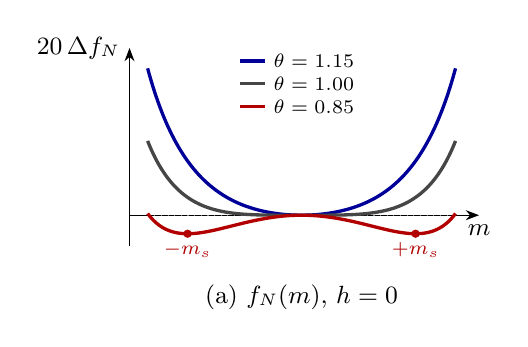
\begin{tikzpicture}[>=Stealth,font=\small,x=2.30cm,y=0.72cm]
  \draw[->] (-0.95,0) -- (0.98,0) node[below]{$m$};
  \draw[->] (-0.95,-0.55) -- (-0.95,2.95) node[left]{$20\,\Delta f_N$};
  \draw[dotted,gray] (-0.85,0) -- (0.85,0);
  \draw[very thick,blue!60!black] plot coordinates{(-0.8500,2.5905) (-0.8406,2.4810) (-0.8311,2.3766) (-0.8217,2.2771) (-0.8122,2.1821) (-0.8028,2.0914) (-0.7933,2.0047) (-0.7839,1.9217) (-0.7744,1.8422) (-0.7650,1.7661) (-0.7556,1.6932) (-0.7461,1.6232) (-0.7367,1.5561) (-0.7272,1.4917) (-0.7178,1.4299) (-0.7083,1.3705) (-0.6989,1.3135) (-0.6894,1.2587) (-0.6800,1.2060) (-0.6706,1.1553) (-0.6611,1.1066) (-0.6517,1.0598) (-0.6422,1.0147) (-0.6328,0.9713) (-0.6233,0.9296) (-0.6139,0.8895) (-0.6044,0.8508) (-0.5950,0.8136) (-0.5856,0.7778) (-0.5761,0.7433) (-0.5667,0.7102) (-0.5572,0.6782) (-0.5478,0.6475) (-0.5383,0.6179) (-0.5289,0.5894) (-0.5194,0.5620) (-0.5100,0.5356) (-0.5006,0.5101) (-0.4911,0.4857) (-0.4817,0.4621) (-0.4722,0.4395) (-0.4628,0.4177) (-0.4533,0.3967) (-0.4439,0.3765) (-0.4344,0.3571) (-0.4250,0.3385) (-0.4156,0.3205) (-0.4061,0.3033) (-0.3967,0.2867) (-0.3872,0.2708) (-0.3778,0.2555) (-0.3683,0.2408) (-0.3589,0.2268) (-0.3494,0.2132) (-0.3400,0.2003) (-0.3306,0.1878) (-0.3211,0.1759) (-0.3117,0.1645) (-0.3022,0.1536) (-0.2928,0.1432) (-0.2833,0.1332) (-0.2739,0.1236) (-0.2644,0.1145) (-0.2550,0.1059) (-0.2456,0.0976) (-0.2361,0.0897) (-0.2267,0.0822) (-0.2172,0.0751) (-0.2078,0.0684) (-0.1983,0.0620) (-0.1889,0.0560) (-0.1794,0.0503) (-0.1700,0.0450) (-0.1606,0.0400) (-0.1511,0.0353) (-0.1417,0.0309) (-0.1322,0.0268) (-0.1228,0.0230) (-0.1133,0.0196) (-0.1039,0.0164) (-0.0944,0.0135) (-0.0850,0.0109) (-0.0756,0.0086) (-0.0661,0.0066) (-0.0567,0.0048) (-0.0472,0.0034) (-0.0378,0.0021) (-0.0283,0.0012) (-0.0189,0.0005) (-0.0094,0.0001) (0.0000,0.0000) (0.0094,0.0001) (0.0189,0.0005) (0.0283,0.0012) (0.0378,0.0021) (0.0472,0.0034) (0.0567,0.0048) (0.0661,0.0066) (0.0756,0.0086) (0.0850,0.0109) (0.0944,0.0135) (0.1039,0.0164) (0.1133,0.0196) (0.1228,0.0230) (0.1322,0.0268) (0.1417,0.0309) (0.1511,0.0353) (0.1606,0.0400) (0.1700,0.0450) (0.1794,0.0503) (0.1889,0.0560) (0.1983,0.0620) (0.2078,0.0684) (0.2172,0.0751) (0.2267,0.0822) (0.2361,0.0897) (0.2456,0.0976) (0.2550,0.1059) (0.2644,0.1145) (0.2739,0.1236) (0.2833,0.1332) (0.2928,0.1432) (0.3022,0.1536) (0.3117,0.1645) (0.3211,0.1759) (0.3306,0.1878) (0.3400,0.2003) (0.3494,0.2132) (0.3589,0.2268) (0.3683,0.2408) (0.3778,0.2555) (0.3872,0.2708) (0.3967,0.2867) (0.4061,0.3033) (0.4156,0.3205) (0.4250,0.3385) (0.4344,0.3571) (0.4439,0.3765) (0.4533,0.3967) (0.4628,0.4177) (0.4722,0.4395) (0.4817,0.4621) (0.4911,0.4857) (0.5006,0.5101) (0.5100,0.5356) (0.5194,0.5620) (0.5289,0.5894) (0.5383,0.6179) (0.5478,0.6475) (0.5572,0.6782) (0.5667,0.7102) (0.5761,0.7433) (0.5856,0.7778) (0.5950,0.8136) (0.6044,0.8508) (0.6139,0.8895) (0.6233,0.9296) (0.6328,0.9713) (0.6422,1.0147) (0.6517,1.0598) (0.6611,1.1066) (0.6706,1.1553) (0.6800,1.2060) (0.6894,1.2587) (0.6989,1.3135) (0.7083,1.3705) (0.7178,1.4299) (0.7272,1.4917) (0.7367,1.5561) (0.7461,1.6232) (0.7556,1.6932) (0.7650,1.7661) (0.7744,1.8422) (0.7839,1.9217) (0.7933,2.0047) (0.8028,2.0914) (0.8122,2.1821) (0.8217,2.2771) (0.8311,2.3766) (0.8406,2.4810) (0.8500,2.5905)};
  \draw[very thick,gray!55!black] plot coordinates{(-0.8500,1.3103) (-0.8406,1.2358) (-0.8311,1.1656) (-0.8217,1.0995) (-0.8122,1.0370) (-0.8028,0.9780) (-0.7933,0.9222) (-0.7839,0.8695) (-0.7744,0.8196) (-0.7650,0.7724) (-0.7556,0.7277) (-0.7461,0.6854) (-0.7367,0.6453) (-0.7272,0.6073) (-0.7178,0.5714) (-0.7083,0.5373) (-0.6989,0.5051) (-0.6894,0.4745) (-0.6800,0.4455) (-0.6706,0.4181) (-0.6611,0.3922) (-0.6517,0.3676) (-0.6422,0.3444) (-0.6328,0.3224) (-0.6233,0.3016) (-0.6139,0.2819) (-0.6044,0.2633) (-0.5950,0.2457) (-0.5856,0.2291) (-0.5761,0.2135) (-0.5667,0.1987) (-0.5572,0.1848) (-0.5478,0.1716) (-0.5383,0.1593) (-0.5289,0.1477) (-0.5194,0.1367) (-0.5100,0.1264) (-0.5006,0.1168) (-0.4911,0.1077) (-0.4817,0.0992) (-0.4722,0.0913) (-0.4628,0.0839) (-0.4533,0.0769) (-0.4439,0.0704) (-0.4344,0.0644) (-0.4250,0.0587) (-0.4156,0.0535) (-0.4061,0.0486) (-0.3967,0.0441) (-0.3872,0.0399) (-0.3778,0.0360) (-0.3683,0.0325) (-0.3589,0.0292) (-0.3494,0.0262) (-0.3400,0.0234) (-0.3306,0.0208) (-0.3211,0.0185) (-0.3117,0.0164) (-0.3022,0.0144) (-0.2928,0.0127) (-0.2833,0.0111) (-0.2739,0.0097) (-0.2644,0.0084) (-0.2550,0.0072) (-0.2456,0.0062) (-0.2361,0.0053) (-0.2267,0.0045) (-0.2172,0.0038) (-0.2078,0.0032) (-0.1983,0.0026) (-0.1889,0.0022) (-0.1794,0.0018) (-0.1700,0.0014) (-0.1606,0.0011) (-0.1511,0.0009) (-0.1417,0.0007) (-0.1322,0.0005) (-0.1228,0.0004) (-0.1133,0.0003) (-0.1039,0.0002) (-0.0944,0.0001) (-0.0850,0.0001) (-0.0756,0.0001) (-0.0661,0.0000) (-0.0567,0.0000) (-0.0472,0.0000) (-0.0378,0.0000) (-0.0283,0.0000) (-0.0189,0.0000) (-0.0094,0.0000) (0.0000,0.0000) (0.0094,0.0000) (0.0189,0.0000) (0.0283,0.0000) (0.0378,0.0000) (0.0472,0.0000) (0.0567,0.0000) (0.0661,0.0000) (0.0756,0.0001) (0.0850,0.0001) (0.0944,0.0001) (0.1039,0.0002) (0.1133,0.0003) (0.1228,0.0004) (0.1322,0.0005) (0.1417,0.0007) (0.1511,0.0009) (0.1606,0.0011) (0.1700,0.0014) (0.1794,0.0018) (0.1889,0.0022) (0.1983,0.0026) (0.2078,0.0032) (0.2172,0.0038) (0.2267,0.0045) (0.2361,0.0053) (0.2456,0.0062) (0.2550,0.0072) (0.2644,0.0084) (0.2739,0.0097) (0.2833,0.0111) (0.2928,0.0127) (0.3022,0.0144) (0.3117,0.0164) (0.3211,0.0185) (0.3306,0.0208) (0.3400,0.0234) (0.3494,0.0262) (0.3589,0.0292) (0.3683,0.0325) (0.3778,0.0360) (0.3872,0.0399) (0.3967,0.0441) (0.4061,0.0486) (0.4156,0.0535) (0.4250,0.0587) (0.4344,0.0644) (0.4439,0.0704) (0.4533,0.0769) (0.4628,0.0839) (0.4722,0.0913) (0.4817,0.0992) (0.4911,0.1077) (0.5006,0.1168) (0.5100,0.1264) (0.5194,0.1367) (0.5289,0.1477) (0.5383,0.1593) (0.5478,0.1716) (0.5572,0.1848) (0.5667,0.1987) (0.5761,0.2135) (0.5856,0.2291) (0.5950,0.2457) (0.6044,0.2633) (0.6139,0.2819) (0.6233,0.3016) (0.6328,0.3224) (0.6422,0.3444) (0.6517,0.3676) (0.6611,0.3922) (0.6706,0.4181) (0.6800,0.4455) (0.6894,0.4745) (0.6989,0.5051) (0.7083,0.5373) (0.7178,0.5714) (0.7272,0.6073) (0.7367,0.6453) (0.7461,0.6854) (0.7556,0.7277) (0.7650,0.7724) (0.7744,0.8196) (0.7839,0.8695) (0.7933,0.9222) (0.8028,0.9780) (0.8122,1.0370) (0.8217,1.0995) (0.8311,1.1656) (0.8406,1.2358) (0.8500,1.3103)};
  \draw[very thick,red!70!black] plot coordinates{(-0.8500,0.0300) (-0.8406,-0.0094) (-0.8311,-0.0453) (-0.8217,-0.0782) (-0.8122,-0.1081) (-0.8028,-0.1354) (-0.7933,-0.1602) (-0.7839,-0.1826) (-0.7744,-0.2030) (-0.7650,-0.2213) (-0.7556,-0.2377) (-0.7461,-0.2524) (-0.7367,-0.2655) (-0.7272,-0.2770) (-0.7178,-0.2871) (-0.7083,-0.2959) (-0.6989,-0.3034) (-0.6894,-0.3097) (-0.6800,-0.3149) (-0.6706,-0.3191) (-0.6611,-0.3222) (-0.6517,-0.3245) (-0.6422,-0.3260) (-0.6328,-0.3266) (-0.6233,-0.3265) (-0.6139,-0.3257) (-0.6044,-0.3242) (-0.5950,-0.3222) (-0.5856,-0.3196) (-0.5761,-0.3164) (-0.5667,-0.3128) (-0.5572,-0.3087) (-0.5478,-0.3042) (-0.5383,-0.2993) (-0.5289,-0.2941) (-0.5194,-0.2885) (-0.5100,-0.2827) (-0.5006,-0.2766) (-0.4911,-0.2702) (-0.4817,-0.2636) (-0.4722,-0.2569) (-0.4628,-0.2500) (-0.4533,-0.2429) (-0.4439,-0.2357) (-0.4344,-0.2284) (-0.4250,-0.2210) (-0.4156,-0.2136) (-0.4061,-0.2061) (-0.3967,-0.1985) (-0.3872,-0.1910) (-0.3778,-0.1834) (-0.3683,-0.1759) (-0.3589,-0.1684) (-0.3494,-0.1609) (-0.3400,-0.1535) (-0.3306,-0.1462) (-0.3211,-0.1389) (-0.3117,-0.1318) (-0.3022,-0.1247) (-0.2928,-0.1178) (-0.2833,-0.1110) (-0.2739,-0.1043) (-0.2644,-0.0978) (-0.2550,-0.0914) (-0.2456,-0.0852) (-0.2361,-0.0791) (-0.2267,-0.0732) (-0.2172,-0.0676) (-0.2078,-0.0621) (-0.1983,-0.0568) (-0.1889,-0.0517) (-0.1794,-0.0468) (-0.1700,-0.0422) (-0.1606,-0.0377) (-0.1511,-0.0335) (-0.1417,-0.0295) (-0.1322,-0.0258) (-0.1228,-0.0223) (-0.1133,-0.0190) (-0.1039,-0.0160) (-0.0944,-0.0133) (-0.0850,-0.0108) (-0.0756,-0.0085) (-0.0661,-0.0065) (-0.0567,-0.0048) (-0.0472,-0.0033) (-0.0378,-0.0021) (-0.0283,-0.0012) (-0.0189,-0.0005) (-0.0094,-0.0001) (0.0000,0.0000) (0.0094,-0.0001) (0.0189,-0.0005) (0.0283,-0.0012) (0.0378,-0.0021) (0.0472,-0.0033) (0.0567,-0.0048) (0.0661,-0.0065) (0.0756,-0.0085) (0.0850,-0.0108) (0.0944,-0.0133) (0.1039,-0.0160) (0.1133,-0.0190) (0.1228,-0.0223) (0.1322,-0.0258) (0.1417,-0.0295) (0.1511,-0.0335) (0.1606,-0.0377) (0.1700,-0.0422) (0.1794,-0.0468) (0.1889,-0.0517) (0.1983,-0.0568) (0.2078,-0.0621) (0.2172,-0.0676) (0.2267,-0.0732) (0.2361,-0.0791) (0.2456,-0.0852) (0.2550,-0.0914) (0.2644,-0.0978) (0.2739,-0.1043) (0.2833,-0.1110) (0.2928,-0.1178) (0.3022,-0.1247) (0.3117,-0.1318) (0.3211,-0.1389) (0.3306,-0.1462) (0.3400,-0.1535) (0.3494,-0.1609) (0.3589,-0.1684) (0.3683,-0.1759) (0.3778,-0.1834) (0.3872,-0.1910) (0.3967,-0.1985) (0.4061,-0.2061) (0.4156,-0.2136) (0.4250,-0.2210) (0.4344,-0.2284) (0.4439,-0.2357) (0.4533,-0.2429) (0.4628,-0.2500) (0.4722,-0.2569) (0.4817,-0.2636) (0.4911,-0.2702) (0.5006,-0.2766) (0.5100,-0.2827) (0.5194,-0.2885) (0.5289,-0.2941) (0.5383,-0.2993) (0.5478,-0.3042) (0.5572,-0.3087) (0.5667,-0.3128) (0.5761,-0.3164) (0.5856,-0.3196) (0.5950,-0.3222) (0.6044,-0.3242) (0.6139,-0.3257) (0.6233,-0.3265) (0.6328,-0.3266) (0.6422,-0.3260) (0.6517,-0.3245) (0.6611,-0.3222) (0.6706,-0.3191) (0.6800,-0.3149) (0.6894,-0.3097) (0.6989,-0.3034) (0.7083,-0.2959) (0.7178,-0.2871) (0.7272,-0.2770) (0.7367,-0.2655) (0.7461,-0.2524) (0.7556,-0.2377) (0.7650,-0.2213) (0.7744,-0.2030) (0.7839,-0.1826) (0.7933,-0.1602) (0.8028,-0.1354) (0.8122,-0.1081) (0.8217,-0.0782) (0.8311,-0.0453) (0.8406,-0.0094) (0.8500,0.0300)};
  \fill[red!70!black] (0.6295,-0.3266) circle (1.5pt);
  \fill[red!70!black] (-0.6295,-0.3266) circle (1.5pt);
  \node[anchor=north,font=\scriptsize,red!70!black,inner sep=1.5pt] at (0.6295,-0.40) {$+m_s$};
  \node[anchor=north,font=\scriptsize,red!70!black,inner sep=1.5pt] at (-0.6295,-0.40) {$-m_s$};
  \draw[very thick,blue!60!black] (-0.34,2.72) -- (-0.20,2.72);
  \node[anchor=west,font=\scriptsize,inner sep=1.5pt] at (-0.18,2.72) {$\theta=1.15$};
  \draw[very thick,gray!55!black] (-0.34,2.32) -- (-0.20,2.32);
  \node[anchor=west,font=\scriptsize,inner sep=1.5pt] at (-0.18,2.32) {$\theta=1.00$};
  \draw[very thick,red!70!black] (-0.34,1.92) -- (-0.20,1.92);
  \node[anchor=west,font=\scriptsize,inner sep=1.5pt] at (-0.18,1.92) {$\theta=0.85$};
  \node[anchor=north,font=\small] at (0,-1.05) {(a) $f_N(m)$, $h=0$};
\end{tikzpicture}
\hfill
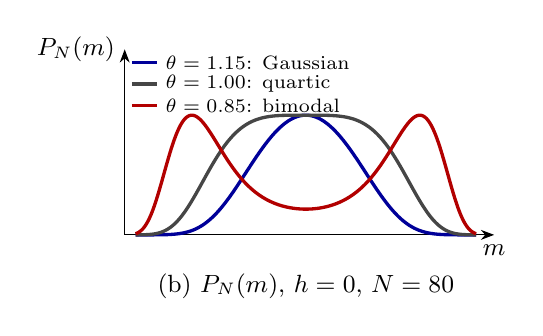
\begin{tikzpicture}[>=Stealth,font=\small,x=2.30cm,y=1.52cm]
  \draw[->] (-1.00,0) -- (1.04,0) node[below]{$m$};
  \draw[->] (-1.00,0) -- (-1.00,1.55) node[left]{$P_N(m)$};
  \draw[very thick,blue!60!black] plot coordinates{(-0.9400,0.0000) (-0.9315,0.0000) (-0.9229,0.0000) (-0.9144,0.0000) (-0.9058,0.0000) (-0.8973,0.0000) (-0.8887,0.0000) (-0.8802,0.0000) (-0.8716,0.0000) (-0.8631,0.0001) (-0.8545,0.0001) (-0.8460,0.0001) (-0.8375,0.0002) (-0.8289,0.0003) (-0.8204,0.0004) (-0.8118,0.0005) (-0.8033,0.0007) (-0.7947,0.0009) (-0.7862,0.0012) (-0.7776,0.0015) (-0.7691,0.0019) (-0.7605,0.0024) (-0.7520,0.0030) (-0.7435,0.0038) (-0.7349,0.0047) (-0.7264,0.0057) (-0.7178,0.0069) (-0.7093,0.0083) (-0.7007,0.0100) (-0.6922,0.0119) (-0.6836,0.0141) (-0.6751,0.0165) (-0.6665,0.0193) (-0.6580,0.0225) (-0.6495,0.0260) (-0.6409,0.0300) (-0.6324,0.0343) (-0.6238,0.0391) (-0.6153,0.0444) (-0.6067,0.0502) (-0.5982,0.0565) (-0.5896,0.0634) (-0.5811,0.0708) (-0.5725,0.0787) (-0.5640,0.0873) (-0.5555,0.0964) (-0.5469,0.1062) (-0.5384,0.1165) (-0.5298,0.1275) (-0.5213,0.1391) (-0.5127,0.1512) (-0.5042,0.1640) (-0.4956,0.1773) (-0.4871,0.1913) (-0.4785,0.2058) (-0.4700,0.2208) (-0.4615,0.2364) (-0.4529,0.2524) (-0.4444,0.2690) (-0.4358,0.2860) (-0.4273,0.3034) (-0.4187,0.3212) (-0.4102,0.3394) (-0.4016,0.3579) (-0.3931,0.3768) (-0.3845,0.3959) (-0.3760,0.4152) (-0.3675,0.4347) (-0.3589,0.4544) (-0.3504,0.4742) (-0.3418,0.4940) (-0.3333,0.5139) (-0.3247,0.5339) (-0.3162,0.5538) (-0.3076,0.5736) (-0.2991,0.5933) (-0.2905,0.6129) (-0.2820,0.6323) (-0.2735,0.6514) (-0.2649,0.6704) (-0.2564,0.6890) (-0.2478,0.7074) (-0.2393,0.7254) (-0.2307,0.7430) (-0.2222,0.7602) (-0.2136,0.7770) (-0.2051,0.7934) (-0.1965,0.8092) (-0.1880,0.8246) (-0.1795,0.8394) (-0.1709,0.8537) (-0.1624,0.8674) (-0.1538,0.8805) (-0.1453,0.8931) (-0.1367,0.9049) (-0.1282,0.9162) (-0.1196,0.9268) (-0.1111,0.9367) (-0.1025,0.9459) (-0.0940,0.9544) (-0.0855,0.9623) (-0.0769,0.9694) (-0.0684,0.9758) (-0.0598,0.9814) (-0.0513,0.9863) (-0.0427,0.9905) (-0.0342,0.9939) (-0.0256,0.9966) (-0.0171,0.9985) (-0.0085,0.9996) (0.0000,1.0000) (0.0085,0.9996) (0.0171,0.9985) (0.0256,0.9966) (0.0342,0.9939) (0.0427,0.9905) (0.0513,0.9863) (0.0598,0.9814) (0.0684,0.9758) (0.0769,0.9694) (0.0855,0.9623) (0.0940,0.9544) (0.1025,0.9459) (0.1111,0.9367) (0.1196,0.9268) (0.1282,0.9162) (0.1367,0.9049) (0.1453,0.8931) (0.1538,0.8805) (0.1624,0.8674) (0.1709,0.8537) (0.1795,0.8394) (0.1880,0.8246) (0.1965,0.8092) (0.2051,0.7934) (0.2136,0.7770) (0.2222,0.7602) (0.2307,0.7430) (0.2393,0.7254) (0.2478,0.7074) (0.2564,0.6890) (0.2649,0.6704) (0.2735,0.6514) (0.2820,0.6323) (0.2905,0.6129) (0.2991,0.5933) (0.3076,0.5736) (0.3162,0.5538) (0.3247,0.5339) (0.3333,0.5139) (0.3418,0.4940) (0.3504,0.4742) (0.3589,0.4544) (0.3675,0.4347) (0.3760,0.4152) (0.3845,0.3959) (0.3931,0.3768) (0.4016,0.3579) (0.4102,0.3394) (0.4187,0.3212) (0.4273,0.3034) (0.4358,0.2860) (0.4444,0.2690) (0.4529,0.2524) (0.4615,0.2364) (0.4700,0.2208) (0.4785,0.2058) (0.4871,0.1913) (0.4956,0.1773) (0.5042,0.1640) (0.5127,0.1512) (0.5213,0.1391) (0.5298,0.1275) (0.5384,0.1165) (0.5469,0.1062) (0.5555,0.0964) (0.5640,0.0873) (0.5725,0.0787) (0.5811,0.0708) (0.5896,0.0634) (0.5982,0.0565) (0.6067,0.0502) (0.6153,0.0444) (0.6238,0.0391) (0.6324,0.0343) (0.6409,0.0300) (0.6495,0.0260) (0.6580,0.0225) (0.6665,0.0193) (0.6751,0.0165) (0.6836,0.0141) (0.6922,0.0119) (0.7007,0.0100) (0.7093,0.0083) (0.7178,0.0069) (0.7264,0.0057) (0.7349,0.0047) (0.7435,0.0038) (0.7520,0.0030) (0.7605,0.0024) (0.7691,0.0019) (0.7776,0.0015) (0.7862,0.0012) (0.7947,0.0009) (0.8033,0.0007) (0.8118,0.0005) (0.8204,0.0004) (0.8289,0.0003) (0.8375,0.0002) (0.8460,0.0001) (0.8545,0.0001) (0.8631,0.0001) (0.8716,0.0000) (0.8802,0.0000) (0.8887,0.0000) (0.8973,0.0000) (0.9058,0.0000) (0.9144,0.0000) (0.9229,0.0000) (0.9315,0.0000) (0.9400,0.0000)};
  \draw[very thick,gray!55!black] plot coordinates{(-0.9400,0.0001) (-0.9315,0.0002) (-0.9229,0.0002) (-0.9144,0.0004) (-0.9058,0.0006) (-0.8973,0.0009) (-0.8887,0.0013) (-0.8802,0.0018) (-0.8716,0.0025) (-0.8631,0.0034) (-0.8545,0.0046) (-0.8460,0.0060) (-0.8375,0.0078) (-0.8289,0.0101) (-0.8204,0.0127) (-0.8118,0.0160) (-0.8033,0.0198) (-0.7947,0.0242) (-0.7862,0.0294) (-0.7776,0.0353) (-0.7691,0.0420) (-0.7605,0.0496) (-0.7520,0.0581) (-0.7435,0.0675) (-0.7349,0.0779) (-0.7264,0.0893) (-0.7178,0.1017) (-0.7093,0.1150) (-0.7007,0.1294) (-0.6922,0.1448) (-0.6836,0.1611) (-0.6751,0.1783) (-0.6665,0.1964) (-0.6580,0.2153) (-0.6495,0.2350) (-0.6409,0.2554) (-0.6324,0.2765) (-0.6238,0.2981) (-0.6153,0.3202) (-0.6067,0.3428) (-0.5982,0.3656) (-0.5896,0.3888) (-0.5811,0.4121) (-0.5725,0.4355) (-0.5640,0.4590) (-0.5555,0.4824) (-0.5469,0.5056) (-0.5384,0.5287) (-0.5298,0.5515) (-0.5213,0.5740) (-0.5127,0.5961) (-0.5042,0.6177) (-0.4956,0.6389) (-0.4871,0.6595) (-0.4785,0.6796) (-0.4700,0.6991) (-0.4615,0.7179) (-0.4529,0.7361) (-0.4444,0.7536) (-0.4358,0.7704) (-0.4273,0.7865) (-0.4187,0.8018) (-0.4102,0.8165) (-0.4016,0.8305) (-0.3931,0.8437) (-0.3845,0.8563) (-0.3760,0.8681) (-0.3675,0.8793) (-0.3589,0.8898) (-0.3504,0.8997) (-0.3418,0.9089) (-0.3333,0.9175) (-0.3247,0.9255) (-0.3162,0.9329) (-0.3076,0.9398) (-0.2991,0.9461) (-0.2905,0.9520) (-0.2820,0.9574) (-0.2735,0.9623) (-0.2649,0.9668) (-0.2564,0.9709) (-0.2478,0.9745) (-0.2393,0.9779) (-0.2307,0.9809) (-0.2222,0.9836) (-0.2136,0.9860) (-0.2051,0.9881) (-0.1965,0.9899) (-0.1880,0.9916) (-0.1795,0.9930) (-0.1709,0.9943) (-0.1624,0.9953) (-0.1538,0.9962) (-0.1453,0.9970) (-0.1367,0.9977) (-0.1282,0.9982) (-0.1196,0.9986) (-0.1111,0.9990) (-0.1025,0.9993) (-0.0940,0.9995) (-0.0855,0.9996) (-0.0769,0.9998) (-0.0684,0.9999) (-0.0598,0.9999) (-0.0513,1.0000) (-0.0427,1.0000) (-0.0342,1.0000) (-0.0256,1.0000) (-0.0171,1.0000) (-0.0085,1.0000) (0.0000,1.0000) (0.0085,1.0000) (0.0171,1.0000) (0.0256,1.0000) (0.0342,1.0000) (0.0427,1.0000) (0.0513,1.0000) (0.0598,0.9999) (0.0684,0.9999) (0.0769,0.9998) (0.0855,0.9996) (0.0940,0.9995) (0.1025,0.9993) (0.1111,0.9990) (0.1196,0.9986) (0.1282,0.9982) (0.1367,0.9977) (0.1453,0.9970) (0.1538,0.9962) (0.1624,0.9953) (0.1709,0.9943) (0.1795,0.9930) (0.1880,0.9916) (0.1965,0.9899) (0.2051,0.9881) (0.2136,0.9860) (0.2222,0.9836) (0.2307,0.9809) (0.2393,0.9779) (0.2478,0.9745) (0.2564,0.9709) (0.2649,0.9668) (0.2735,0.9623) (0.2820,0.9574) (0.2905,0.9520) (0.2991,0.9461) (0.3076,0.9398) (0.3162,0.9329) (0.3247,0.9255) (0.3333,0.9175) (0.3418,0.9089) (0.3504,0.8997) (0.3589,0.8898) (0.3675,0.8793) (0.3760,0.8681) (0.3845,0.8563) (0.3931,0.8437) (0.4016,0.8305) (0.4102,0.8165) (0.4187,0.8018) (0.4273,0.7865) (0.4358,0.7704) (0.4444,0.7536) (0.4529,0.7361) (0.4615,0.7179) (0.4700,0.6991) (0.4785,0.6796) (0.4871,0.6595) (0.4956,0.6389) (0.5042,0.6177) (0.5127,0.5961) (0.5213,0.5740) (0.5298,0.5515) (0.5384,0.5287) (0.5469,0.5056) (0.5555,0.4824) (0.5640,0.4590) (0.5725,0.4355) (0.5811,0.4121) (0.5896,0.3888) (0.5982,0.3656) (0.6067,0.3428) (0.6153,0.3202) (0.6238,0.2981) (0.6324,0.2765) (0.6409,0.2554) (0.6495,0.2350) (0.6580,0.2153) (0.6665,0.1964) (0.6751,0.1783) (0.6836,0.1611) (0.6922,0.1448) (0.7007,0.1294) (0.7093,0.1150) (0.7178,0.1017) (0.7264,0.0893) (0.7349,0.0779) (0.7435,0.0675) (0.7520,0.0581) (0.7605,0.0496) (0.7691,0.0420) (0.7776,0.0353) (0.7862,0.0294) (0.7947,0.0242) (0.8033,0.0198) (0.8118,0.0160) (0.8204,0.0127) (0.8289,0.0101) (0.8375,0.0078) (0.8460,0.0060) (0.8545,0.0046) (0.8631,0.0034) (0.8716,0.0025) (0.8802,0.0018) (0.8887,0.0013) (0.8973,0.0009) (0.9058,0.0006) (0.9144,0.0004) (0.9229,0.0002) (0.9315,0.0002) (0.9400,0.0001)};
  \draw[very thick,red!70!black] plot coordinates{(-0.9400,0.0098) (-0.9315,0.0147) (-0.9229,0.0214) (-0.9144,0.0302) (-0.9058,0.0412) (-0.8973,0.0550) (-0.8887,0.0716) (-0.8802,0.0913) (-0.8716,0.1142) (-0.8631,0.1403) (-0.8545,0.1698) (-0.8460,0.2024) (-0.8375,0.2379) (-0.8289,0.2762) (-0.8204,0.3169) (-0.8118,0.3596) (-0.8033,0.4039) (-0.7947,0.4493) (-0.7862,0.4954) (-0.7776,0.5416) (-0.7691,0.5874) (-0.7605,0.6324) (-0.7520,0.6761) (-0.7435,0.7181) (-0.7349,0.7580) (-0.7264,0.7954) (-0.7178,0.8301) (-0.7093,0.8619) (-0.7007,0.8905) (-0.6922,0.9159) (-0.6836,0.9378) (-0.6751,0.9564) (-0.6665,0.9716) (-0.6580,0.9834) (-0.6495,0.9920) (-0.6409,0.9974) (-0.6324,0.9998) (-0.6238,0.9994) (-0.6153,0.9963) (-0.6067,0.9906) (-0.5982,0.9827) (-0.5896,0.9726) (-0.5811,0.9607) (-0.5725,0.9471) (-0.5640,0.9319) (-0.5555,0.9155) (-0.5469,0.8979) (-0.5384,0.8793) (-0.5298,0.8600) (-0.5213,0.8401) (-0.5127,0.8197) (-0.5042,0.7989) (-0.4956,0.7779) (-0.4871,0.7568) (-0.4785,0.7357) (-0.4700,0.7147) (-0.4615,0.6939) (-0.4529,0.6732) (-0.4444,0.6529) (-0.4358,0.6330) (-0.4273,0.6134) (-0.4187,0.5943) (-0.4102,0.5757) (-0.4016,0.5575) (-0.3931,0.5399) (-0.3845,0.5228) (-0.3760,0.5063) (-0.3675,0.4903) (-0.3589,0.4749) (-0.3504,0.4601) (-0.3418,0.4458) (-0.3333,0.4320) (-0.3247,0.4188) (-0.3162,0.4062) (-0.3076,0.3941) (-0.2991,0.3825) (-0.2905,0.3714) (-0.2820,0.3608) (-0.2735,0.3507) (-0.2649,0.3411) (-0.2564,0.3319) (-0.2478,0.3232) (-0.2393,0.3149) (-0.2307,0.3071) (-0.2222,0.2996) (-0.2136,0.2925) (-0.2051,0.2859) (-0.1965,0.2795) (-0.1880,0.2736) (-0.1795,0.2680) (-0.1709,0.2627) (-0.1624,0.2577) (-0.1538,0.2531) (-0.1453,0.2488) (-0.1367,0.2447) (-0.1282,0.2410) (-0.1196,0.2375) (-0.1111,0.2343) (-0.1025,0.2314) (-0.0940,0.2287) (-0.0855,0.2263) (-0.0769,0.2241) (-0.0684,0.2222) (-0.0598,0.2205) (-0.0513,0.2190) (-0.0427,0.2178) (-0.0342,0.2168) (-0.0256,0.2160) (-0.0171,0.2154) (-0.0085,0.2151) (0.0000,0.2150) (0.0085,0.2151) (0.0171,0.2154) (0.0256,0.2160) (0.0342,0.2168) (0.0427,0.2178) (0.0513,0.2190) (0.0598,0.2205) (0.0684,0.2222) (0.0769,0.2241) (0.0855,0.2263) (0.0940,0.2287) (0.1025,0.2314) (0.1111,0.2343) (0.1196,0.2375) (0.1282,0.2410) (0.1367,0.2447) (0.1453,0.2488) (0.1538,0.2531) (0.1624,0.2577) (0.1709,0.2627) (0.1795,0.2680) (0.1880,0.2736) (0.1965,0.2795) (0.2051,0.2859) (0.2136,0.2925) (0.2222,0.2996) (0.2307,0.3071) (0.2393,0.3149) (0.2478,0.3232) (0.2564,0.3319) (0.2649,0.3411) (0.2735,0.3507) (0.2820,0.3608) (0.2905,0.3714) (0.2991,0.3825) (0.3076,0.3941) (0.3162,0.4062) (0.3247,0.4188) (0.3333,0.4320) (0.3418,0.4458) (0.3504,0.4601) (0.3589,0.4749) (0.3675,0.4903) (0.3760,0.5063) (0.3845,0.5228) (0.3931,0.5399) (0.4016,0.5575) (0.4102,0.5757) (0.4187,0.5943) (0.4273,0.6134) (0.4358,0.6330) (0.4444,0.6529) (0.4529,0.6732) (0.4615,0.6939) (0.4700,0.7147) (0.4785,0.7357) (0.4871,0.7568) (0.4956,0.7779) (0.5042,0.7989) (0.5127,0.8197) (0.5213,0.8401) (0.5298,0.8600) (0.5384,0.8793) (0.5469,0.8979) (0.5555,0.9155) (0.5640,0.9319) (0.5725,0.9471) (0.5811,0.9607) (0.5896,0.9726) (0.5982,0.9827) (0.6067,0.9906) (0.6153,0.9963) (0.6238,0.9994) (0.6324,0.9998) (0.6409,0.9974) (0.6495,0.9920) (0.6580,0.9834) (0.6665,0.9716) (0.6751,0.9564) (0.6836,0.9378) (0.6922,0.9159) (0.7007,0.8905) (0.7093,0.8619) (0.7178,0.8301) (0.7264,0.7954) (0.7349,0.7580) (0.7435,0.7181) (0.7520,0.6761) (0.7605,0.6324) (0.7691,0.5874) (0.7776,0.5416) (0.7862,0.4954) (0.7947,0.4493) (0.8033,0.4039) (0.8118,0.3596) (0.8204,0.3169) (0.8289,0.2762) (0.8375,0.2379) (0.8460,0.2024) (0.8545,0.1698) (0.8631,0.1403) (0.8716,0.1142) (0.8802,0.0913) (0.8887,0.0716) (0.8973,0.0550) (0.9058,0.0412) (0.9144,0.0302) (0.9229,0.0214) (0.9315,0.0147) (0.9400,0.0098)};
  \draw[very thick,blue!60!black] (-0.96,1.44) -- (-0.82,1.44);
  \node[anchor=west,font=\scriptsize,inner sep=1.5pt] at (-0.80,1.44) {$\theta=1.15$: Gaussian};
  \draw[very thick,gray!55!black] (-0.96,1.26) -- (-0.82,1.26);
  \node[anchor=west,font=\scriptsize,inner sep=1.5pt] at (-0.80,1.26) {$\theta=1.00$: quartic};
  \draw[very thick,red!70!black] (-0.96,1.08) -- (-0.82,1.08);
  \node[anchor=west,font=\scriptsize,inner sep=1.5pt] at (-0.80,1.08) {$\theta=0.85$: bimodal};
  \node[anchor=north,font=\small] at (0,-0.24) {(b) $P_N(m)$, $h=0$, $N=80$};
\end{tikzpicture}

\vspace{3ex}
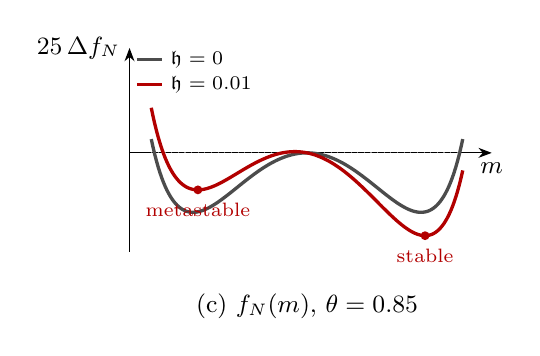
\begin{tikzpicture}[>=Stealth,font=\small,x=2.30cm,y=1.85cm]
  \draw[->] (-0.98,0) -- (1.02,0) node[below]{$m$};
  \draw[->] (-0.98,-0.68) -- (-0.98,0.72) node[left]{$25\,\Delta f_N$};
  \draw[dotted,gray] (-0.86,0) -- (0.86,0);
  \draw[very thick,gray!60!black] plot coordinates{(-0.8600,0.0945) (-0.8504,0.0399) (-0.8409,-0.0101) (-0.8313,-0.0556) (-0.8218,-0.0972) (-0.8122,-0.1351) (-0.8027,-0.1696) (-0.7931,-0.2009) (-0.7836,-0.2292) (-0.7740,-0.2548) (-0.7644,-0.2779) (-0.7549,-0.2985) (-0.7453,-0.3170) (-0.7358,-0.3333) (-0.7262,-0.3477) (-0.7167,-0.3603) (-0.7071,-0.3711) (-0.6976,-0.3804) (-0.6880,-0.3882) (-0.6784,-0.3946) (-0.6689,-0.3996) (-0.6593,-0.4034) (-0.6498,-0.4061) (-0.6402,-0.4077) (-0.6307,-0.4083) (-0.6211,-0.4080) (-0.6116,-0.4067) (-0.6020,-0.4047) (-0.5924,-0.4019) (-0.5829,-0.3984) (-0.5733,-0.3942) (-0.5638,-0.3895) (-0.5542,-0.3841) (-0.5447,-0.3783) (-0.5351,-0.3720) (-0.5256,-0.3652) (-0.5160,-0.3580) (-0.5064,-0.3505) (-0.4969,-0.3427) (-0.4873,-0.3345) (-0.4778,-0.3261) (-0.4682,-0.3175) (-0.4587,-0.3086) (-0.4491,-0.2996) (-0.4396,-0.2905) (-0.4300,-0.2812) (-0.4204,-0.2718) (-0.4109,-0.2623) (-0.4013,-0.2528) (-0.3918,-0.2433) (-0.3822,-0.2337) (-0.3727,-0.2242) (-0.3631,-0.2147) (-0.3536,-0.2052) (-0.3440,-0.1958) (-0.3344,-0.1865) (-0.3249,-0.1773) (-0.3153,-0.1682) (-0.3058,-0.1592) (-0.2962,-0.1504) (-0.2867,-0.1417) (-0.2771,-0.1332) (-0.2676,-0.1249) (-0.2580,-0.1167) (-0.2484,-0.1088) (-0.2389,-0.1011) (-0.2293,-0.0936) (-0.2198,-0.0864) (-0.2102,-0.0793) (-0.2007,-0.0726) (-0.1911,-0.0661) (-0.1816,-0.0599) (-0.1720,-0.0539) (-0.1624,-0.0482) (-0.1529,-0.0429) (-0.1433,-0.0378) (-0.1338,-0.0330) (-0.1242,-0.0285) (-0.1147,-0.0243) (-0.1051,-0.0205) (-0.0956,-0.0170) (-0.0860,-0.0138) (-0.0764,-0.0109) (-0.0669,-0.0084) (-0.0573,-0.0061) (-0.0478,-0.0043) (-0.0382,-0.0027) (-0.0287,-0.0015) (-0.0191,-0.0007) (-0.0096,-0.0002) (0.0000,0.0000) (0.0096,-0.0002) (0.0191,-0.0007) (0.0287,-0.0015) (0.0382,-0.0027) (0.0478,-0.0043) (0.0573,-0.0061) (0.0669,-0.0084) (0.0764,-0.0109) (0.0860,-0.0138) (0.0956,-0.0170) (0.1051,-0.0205) (0.1147,-0.0243) (0.1242,-0.0285) (0.1338,-0.0330) (0.1433,-0.0378) (0.1529,-0.0429) (0.1624,-0.0482) (0.1720,-0.0539) (0.1816,-0.0599) (0.1911,-0.0661) (0.2007,-0.0726) (0.2102,-0.0793) (0.2198,-0.0864) (0.2293,-0.0936) (0.2389,-0.1011) (0.2484,-0.1088) (0.2580,-0.1167) (0.2676,-0.1249) (0.2771,-0.1332) (0.2867,-0.1417) (0.2962,-0.1504) (0.3058,-0.1592) (0.3153,-0.1682) (0.3249,-0.1773) (0.3344,-0.1865) (0.3440,-0.1958) (0.3536,-0.2052) (0.3631,-0.2147) (0.3727,-0.2242) (0.3822,-0.2337) (0.3918,-0.2433) (0.4013,-0.2528) (0.4109,-0.2623) (0.4204,-0.2718) (0.4300,-0.2812) (0.4396,-0.2905) (0.4491,-0.2996) (0.4587,-0.3086) (0.4682,-0.3175) (0.4778,-0.3261) (0.4873,-0.3345) (0.4969,-0.3427) (0.5064,-0.3505) (0.5160,-0.3580) (0.5256,-0.3652) (0.5351,-0.3720) (0.5447,-0.3783) (0.5542,-0.3841) (0.5638,-0.3895) (0.5733,-0.3942) (0.5829,-0.3984) (0.5924,-0.4019) (0.6020,-0.4047) (0.6116,-0.4067) (0.6211,-0.4080) (0.6307,-0.4083) (0.6402,-0.4077) (0.6498,-0.4061) (0.6593,-0.4034) (0.6689,-0.3996) (0.6784,-0.3946) (0.6880,-0.3882) (0.6976,-0.3804) (0.7071,-0.3711) (0.7167,-0.3603) (0.7262,-0.3477) (0.7358,-0.3333) (0.7453,-0.3170) (0.7549,-0.2985) (0.7644,-0.2779) (0.7740,-0.2548) (0.7836,-0.2292) (0.7931,-0.2009) (0.8027,-0.1696) (0.8122,-0.1351) (0.8218,-0.0972) (0.8313,-0.0556) (0.8409,-0.0101) (0.8504,0.0399) (0.8600,0.0945)};
  \draw[very thick,red!70!black] plot coordinates{(-0.8600,0.3095) (-0.8504,0.2525) (-0.8409,0.2002) (-0.8313,0.1522) (-0.8218,0.1082) (-0.8122,0.0679) (-0.8027,0.0311) (-0.7931,-0.0026) (-0.7836,-0.0333) (-0.7740,-0.0613) (-0.7644,-0.0868) (-0.7549,-0.1098) (-0.7453,-0.1306) (-0.7358,-0.1494) (-0.7262,-0.1662) (-0.7167,-0.1811) (-0.7071,-0.1944) (-0.6976,-0.2060) (-0.6880,-0.2162) (-0.6784,-0.2249) (-0.6689,-0.2324) (-0.6593,-0.2386) (-0.6498,-0.2437) (-0.6402,-0.2477) (-0.6307,-0.2506) (-0.6211,-0.2527) (-0.6116,-0.2538) (-0.6020,-0.2542) (-0.5924,-0.2538) (-0.5829,-0.2527) (-0.5733,-0.2509) (-0.5638,-0.2485) (-0.5542,-0.2456) (-0.5447,-0.2421) (-0.5351,-0.2382) (-0.5256,-0.2338) (-0.5160,-0.2290) (-0.5064,-0.2239) (-0.4969,-0.2184) (-0.4873,-0.2127) (-0.4778,-0.2067) (-0.4682,-0.2004) (-0.4587,-0.1940) (-0.4491,-0.1873) (-0.4396,-0.1806) (-0.4300,-0.1737) (-0.4204,-0.1667) (-0.4109,-0.1596) (-0.4013,-0.1525) (-0.3918,-0.1453) (-0.3822,-0.1382) (-0.3727,-0.1310) (-0.3631,-0.1239) (-0.3536,-0.1168) (-0.3440,-0.1098) (-0.3344,-0.1029) (-0.3249,-0.0961) (-0.3153,-0.0894) (-0.3058,-0.0828) (-0.2962,-0.0763) (-0.2867,-0.0700) (-0.2771,-0.0639) (-0.2676,-0.0580) (-0.2580,-0.0522) (-0.2484,-0.0467) (-0.2389,-0.0414) (-0.2293,-0.0363) (-0.2198,-0.0314) (-0.2102,-0.0268) (-0.2007,-0.0224) (-0.1911,-0.0183) (-0.1816,-0.0145) (-0.1720,-0.0109) (-0.1624,-0.0076) (-0.1529,-0.0046) (-0.1433,-0.0019) (-0.1338,0.0005) (-0.1242,0.0025) (-0.1147,0.0043) (-0.1051,0.0058) (-0.0956,0.0069) (-0.0860,0.0077) (-0.0764,0.0082) (-0.0669,0.0084) (-0.0573,0.0082) (-0.0478,0.0077) (-0.0382,0.0068) (-0.0287,0.0056) (-0.0191,0.0041) (-0.0096,0.0022) (0.0000,0.0000) (0.0096,-0.0026) (0.0191,-0.0055) (0.0287,-0.0087) (0.0382,-0.0123) (0.0478,-0.0162) (0.0573,-0.0205) (0.0669,-0.0251) (0.0764,-0.0300) (0.0860,-0.0353) (0.0956,-0.0409) (0.1051,-0.0468) (0.1147,-0.0530) (0.1242,-0.0596) (0.1338,-0.0664) (0.1433,-0.0736) (0.1529,-0.0811) (0.1624,-0.0888) (0.1720,-0.0969) (0.1816,-0.1052) (0.1911,-0.1139) (0.2007,-0.1227) (0.2102,-0.1319) (0.2198,-0.1413) (0.2293,-0.1509) (0.2389,-0.1608) (0.2484,-0.1709) (0.2580,-0.1812) (0.2676,-0.1918) (0.2771,-0.2025) (0.2867,-0.2134) (0.2962,-0.2244) (0.3058,-0.2357) (0.3153,-0.2470) (0.3249,-0.2585) (0.3344,-0.2701) (0.3440,-0.2818) (0.3536,-0.2936) (0.3631,-0.3055) (0.3727,-0.3174) (0.3822,-0.3293) (0.3918,-0.3412) (0.4013,-0.3532) (0.4109,-0.3650) (0.4204,-0.3769) (0.4300,-0.3887) (0.4396,-0.4003) (0.4491,-0.4119) (0.4587,-0.4233) (0.4682,-0.4345) (0.4778,-0.4455) (0.4873,-0.4563) (0.4969,-0.4669) (0.5064,-0.4771) (0.5160,-0.4870) (0.5256,-0.4966) (0.5351,-0.5057) (0.5447,-0.5144) (0.5542,-0.5227) (0.5638,-0.5304) (0.5733,-0.5376) (0.5829,-0.5441) (0.5924,-0.5500) (0.6020,-0.5552) (0.6116,-0.5596) (0.6211,-0.5632) (0.6307,-0.5660) (0.6402,-0.5678) (0.6498,-0.5686) (0.6593,-0.5683) (0.6689,-0.5668) (0.6784,-0.5642) (0.6880,-0.5602) (0.6976,-0.5548) (0.7071,-0.5479) (0.7167,-0.5394) (0.7262,-0.5293) (0.7358,-0.5173) (0.7453,-0.5033) (0.7549,-0.4873) (0.7644,-0.4690) (0.7740,-0.4483) (0.7836,-0.4251) (0.7931,-0.3992) (0.8027,-0.3703) (0.8122,-0.3382) (0.8218,-0.3027) (0.8313,-0.2635) (0.8409,-0.2203) (0.8504,-0.1727) (0.8600,-0.1205)};
  \fill[red!70!black] (0.6520,-0.5686) circle (1.6pt);
  \fill[red!70!black] (-0.6025,-0.2542) circle (1.6pt);
  \node[anchor=north,font=\scriptsize,red!70!black,inner sep=1.5pt] at (-0.6025,-0.31) {metastable};
  \node[anchor=north,font=\scriptsize,red!70!black,inner sep=1.5pt] at (0.6520,-0.63) {stable};
  \draw[very thick,gray!60!black] (-0.94,0.64) -- (-0.80,0.64);
  \node[anchor=west,font=\scriptsize,inner sep=1.5pt] at (-0.78,0.64) {$\mathfrak{h}=0$};
  \draw[very thick,red!70!black] (-0.94,0.47) -- (-0.80,0.47);
  \node[anchor=west,font=\scriptsize,inner sep=1.5pt] at (-0.78,0.47) {$\mathfrak{h}=0.01$};
  \node[anchor=north,font=\small] at (0,-0.90) {(c) $f_N(m)$, $\theta=0.85$};
\end{tikzpicture}
\hfill
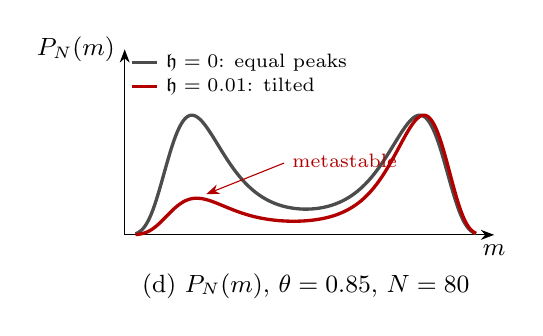
\begin{tikzpicture}[>=Stealth,font=\small,x=2.30cm,y=1.52cm]
  \draw[->] (-1.00,0) -- (1.04,0) node[below]{$m$};
  \draw[->] (-1.00,0) -- (-1.00,1.55) node[left]{$P_N(m)$};
  \draw[very thick,gray!60!black] plot coordinates{(-0.9400,0.0098) (-0.9315,0.0147) (-0.9229,0.0214) (-0.9144,0.0302) (-0.9058,0.0412) (-0.8973,0.0550) (-0.8887,0.0716) (-0.8802,0.0913) (-0.8716,0.1142) (-0.8631,0.1403) (-0.8545,0.1698) (-0.8460,0.2024) (-0.8375,0.2379) (-0.8289,0.2762) (-0.8204,0.3169) (-0.8118,0.3596) (-0.8033,0.4039) (-0.7947,0.4493) (-0.7862,0.4954) (-0.7776,0.5416) (-0.7691,0.5874) (-0.7605,0.6324) (-0.7520,0.6761) (-0.7435,0.7181) (-0.7349,0.7580) (-0.7264,0.7954) (-0.7178,0.8301) (-0.7093,0.8619) (-0.7007,0.8905) (-0.6922,0.9159) (-0.6836,0.9378) (-0.6751,0.9564) (-0.6665,0.9716) (-0.6580,0.9834) (-0.6495,0.9920) (-0.6409,0.9974) (-0.6324,0.9998) (-0.6238,0.9994) (-0.6153,0.9963) (-0.6067,0.9906) (-0.5982,0.9827) (-0.5896,0.9726) (-0.5811,0.9607) (-0.5725,0.9471) (-0.5640,0.9319) (-0.5555,0.9155) (-0.5469,0.8979) (-0.5384,0.8793) (-0.5298,0.8600) (-0.5213,0.8401) (-0.5127,0.8197) (-0.5042,0.7989) (-0.4956,0.7779) (-0.4871,0.7568) (-0.4785,0.7357) (-0.4700,0.7147) (-0.4615,0.6939) (-0.4529,0.6732) (-0.4444,0.6529) (-0.4358,0.6330) (-0.4273,0.6134) (-0.4187,0.5943) (-0.4102,0.5757) (-0.4016,0.5575) (-0.3931,0.5399) (-0.3845,0.5228) (-0.3760,0.5063) (-0.3675,0.4903) (-0.3589,0.4749) (-0.3504,0.4601) (-0.3418,0.4458) (-0.3333,0.4320) (-0.3247,0.4188) (-0.3162,0.4062) (-0.3076,0.3941) (-0.2991,0.3825) (-0.2905,0.3714) (-0.2820,0.3608) (-0.2735,0.3507) (-0.2649,0.3411) (-0.2564,0.3319) (-0.2478,0.3232) (-0.2393,0.3149) (-0.2307,0.3071) (-0.2222,0.2996) (-0.2136,0.2925) (-0.2051,0.2859) (-0.1965,0.2795) (-0.1880,0.2736) (-0.1795,0.2680) (-0.1709,0.2627) (-0.1624,0.2577) (-0.1538,0.2531) (-0.1453,0.2488) (-0.1367,0.2447) (-0.1282,0.2410) (-0.1196,0.2375) (-0.1111,0.2343) (-0.1025,0.2314) (-0.0940,0.2287) (-0.0855,0.2263) (-0.0769,0.2241) (-0.0684,0.2222) (-0.0598,0.2205) (-0.0513,0.2190) (-0.0427,0.2178) (-0.0342,0.2168) (-0.0256,0.2160) (-0.0171,0.2154) (-0.0085,0.2151) (0.0000,0.2150) (0.0085,0.2151) (0.0171,0.2154) (0.0256,0.2160) (0.0342,0.2168) (0.0427,0.2178) (0.0513,0.2190) (0.0598,0.2205) (0.0684,0.2222) (0.0769,0.2241) (0.0855,0.2263) (0.0940,0.2287) (0.1025,0.2314) (0.1111,0.2343) (0.1196,0.2375) (0.1282,0.2410) (0.1367,0.2447) (0.1453,0.2488) (0.1538,0.2531) (0.1624,0.2577) (0.1709,0.2627) (0.1795,0.2680) (0.1880,0.2736) (0.1965,0.2795) (0.2051,0.2859) (0.2136,0.2925) (0.2222,0.2996) (0.2307,0.3071) (0.2393,0.3149) (0.2478,0.3232) (0.2564,0.3319) (0.2649,0.3411) (0.2735,0.3507) (0.2820,0.3608) (0.2905,0.3714) (0.2991,0.3825) (0.3076,0.3941) (0.3162,0.4062) (0.3247,0.4188) (0.3333,0.4320) (0.3418,0.4458) (0.3504,0.4601) (0.3589,0.4749) (0.3675,0.4903) (0.3760,0.5063) (0.3845,0.5228) (0.3931,0.5399) (0.4016,0.5575) (0.4102,0.5757) (0.4187,0.5943) (0.4273,0.6134) (0.4358,0.6330) (0.4444,0.6529) (0.4529,0.6732) (0.4615,0.6939) (0.4700,0.7147) (0.4785,0.7357) (0.4871,0.7568) (0.4956,0.7779) (0.5042,0.7989) (0.5127,0.8197) (0.5213,0.8401) (0.5298,0.8600) (0.5384,0.8793) (0.5469,0.8979) (0.5555,0.9155) (0.5640,0.9319) (0.5725,0.9471) (0.5811,0.9607) (0.5896,0.9726) (0.5982,0.9827) (0.6067,0.9906) (0.6153,0.9963) (0.6238,0.9994) (0.6324,0.9998) (0.6409,0.9974) (0.6495,0.9920) (0.6580,0.9834) (0.6665,0.9716) (0.6751,0.9564) (0.6836,0.9378) (0.6922,0.9159) (0.7007,0.8905) (0.7093,0.8619) (0.7178,0.8301) (0.7264,0.7954) (0.7349,0.7580) (0.7435,0.7181) (0.7520,0.6761) (0.7605,0.6324) (0.7691,0.5874) (0.7776,0.5416) (0.7862,0.4954) (0.7947,0.4493) (0.8033,0.4039) (0.8118,0.3596) (0.8204,0.3169) (0.8289,0.2762) (0.8375,0.2379) (0.8460,0.2024) (0.8545,0.1698) (0.8631,0.1403) (0.8716,0.1142) (0.8802,0.0913) (0.8887,0.0716) (0.8973,0.0550) (0.9058,0.0412) (0.9144,0.0302) (0.9229,0.0214) (0.9315,0.0147) (0.9400,0.0098)};
  \draw[very thick,red!70!black] plot coordinates{(-0.9400,0.0022) (-0.9315,0.0034) (-0.9229,0.0049) (-0.9144,0.0070) (-0.9058,0.0096) (-0.8973,0.0129) (-0.8887,0.0170) (-0.8802,0.0218) (-0.8716,0.0275) (-0.8631,0.0341) (-0.8545,0.0415) (-0.8460,0.0499) (-0.8375,0.0592) (-0.8289,0.0692) (-0.8204,0.0801) (-0.8118,0.0916) (-0.8033,0.1037) (-0.7947,0.1163) (-0.7862,0.1293) (-0.7776,0.1425) (-0.7691,0.1558) (-0.7605,0.1691) (-0.7520,0.1822) (-0.7435,0.1951) (-0.7349,0.2076) (-0.7264,0.2196) (-0.7178,0.2310) (-0.7093,0.2418) (-0.7007,0.2519) (-0.6922,0.2611) (-0.6836,0.2696) (-0.6751,0.2771) (-0.6665,0.2838) (-0.6580,0.2896) (-0.6495,0.2944) (-0.6409,0.2984) (-0.6324,0.3016) (-0.6238,0.3039) (-0.6153,0.3054) (-0.6067,0.3061) (-0.5982,0.3061) (-0.5896,0.3054) (-0.5811,0.3041) (-0.5725,0.3022) (-0.5640,0.2998) (-0.5555,0.2969) (-0.5469,0.2935) (-0.5384,0.2898) (-0.5298,0.2857) (-0.5213,0.2813) (-0.5127,0.2767) (-0.5042,0.2719) (-0.4956,0.2669) (-0.4871,0.2617) (-0.4785,0.2565) (-0.4700,0.2512) (-0.4615,0.2458) (-0.4529,0.2404) (-0.4444,0.2351) (-0.4358,0.2297) (-0.4273,0.2244) (-0.4187,0.2192) (-0.4102,0.2140) (-0.4016,0.2090) (-0.3931,0.2040) (-0.3845,0.1991) (-0.3760,0.1944) (-0.3675,0.1898) (-0.3589,0.1853) (-0.3504,0.1809) (-0.3418,0.1767) (-0.3333,0.1727) (-0.3247,0.1688) (-0.3162,0.1650) (-0.3076,0.1614) (-0.2991,0.1579) (-0.2905,0.1545) (-0.2820,0.1513) (-0.2735,0.1483) (-0.2649,0.1454) (-0.2564,0.1426) (-0.2478,0.1400) (-0.2393,0.1375) (-0.2307,0.1352) (-0.2222,0.1329) (-0.2136,0.1309) (-0.2051,0.1289) (-0.1965,0.1271) (-0.1880,0.1254) (-0.1795,0.1238) (-0.1709,0.1223) (-0.1624,0.1210) (-0.1538,0.1198) (-0.1453,0.1187) (-0.1367,0.1177) (-0.1282,0.1168) (-0.1196,0.1161) (-0.1111,0.1154) (-0.1025,0.1149) (-0.0940,0.1145) (-0.0855,0.1142) (-0.0769,0.1140) (-0.0684,0.1139) (-0.0598,0.1140) (-0.0513,0.1141) (-0.0427,0.1144) (-0.0342,0.1148) (-0.0256,0.1153) (-0.0171,0.1160) (-0.0085,0.1167) (0.0000,0.1176) (0.0085,0.1186) (0.0171,0.1197) (0.0256,0.1210) (0.0342,0.1224) (0.0427,0.1240) (0.0513,0.1257) (0.0598,0.1276) (0.0684,0.1296) (0.0769,0.1318) (0.0855,0.1341) (0.0940,0.1367) (0.1025,0.1394) (0.1111,0.1423) (0.1196,0.1454) (0.1282,0.1487) (0.1367,0.1522) (0.1453,0.1560) (0.1538,0.1600) (0.1624,0.1643) (0.1709,0.1688) (0.1795,0.1735) (0.1880,0.1786) (0.1965,0.1840) (0.2051,0.1896) (0.2136,0.1956) (0.2222,0.2020) (0.2307,0.2087) (0.2393,0.2158) (0.2478,0.2232) (0.2564,0.2311) (0.2649,0.2394) (0.2735,0.2481) (0.2820,0.2573) (0.2905,0.2670) (0.2991,0.2772) (0.3076,0.2879) (0.3162,0.2992) (0.3247,0.3110) (0.3333,0.3234) (0.3418,0.3363) (0.3504,0.3499) (0.3589,0.3641) (0.3675,0.3790) (0.3760,0.3945) (0.3845,0.4107) (0.3931,0.4275) (0.4016,0.4450) (0.4102,0.4632) (0.4187,0.4821) (0.4273,0.5016) (0.4358,0.5218) (0.4444,0.5426) (0.4529,0.5640) (0.4615,0.5859) (0.4700,0.6084) (0.4785,0.6314) (0.4871,0.6547) (0.4956,0.6784) (0.5042,0.7023) (0.5127,0.7264) (0.5213,0.7505) (0.5298,0.7745) (0.5384,0.7983) (0.5469,0.8217) (0.5555,0.8446) (0.5640,0.8667) (0.5725,0.8879) (0.5811,0.9079) (0.5896,0.9266) (0.5982,0.9438) (0.6067,0.9591) (0.6153,0.9723) (0.6238,0.9833) (0.6324,0.9917) (0.6409,0.9973) (0.6495,0.9998) (0.6580,0.9992) (0.6665,0.9951) (0.6751,0.9875) (0.6836,0.9761) (0.6922,0.9610) (0.7007,0.9419) (0.7093,0.9190) (0.7178,0.8923) (0.7264,0.8619) (0.7349,0.8279) (0.7435,0.7907) (0.7520,0.7505) (0.7605,0.7076) (0.7691,0.6626) (0.7776,0.6158) (0.7862,0.5679) (0.7947,0.5192) (0.8033,0.4705) (0.8118,0.4223) (0.8204,0.3751) (0.8289,0.3296) (0.8375,0.2862) (0.8460,0.2454) (0.8545,0.2075) (0.8631,0.1729) (0.8716,0.1418) (0.8802,0.1143) (0.8887,0.0903) (0.8973,0.0699) (0.9058,0.0529) (0.9144,0.0390) (0.9229,0.0279) (0.9315,0.0194) (0.9400,0.0129)};
  \draw[->,red!70!black,thin] (-0.12,0.60) -- (-0.55,0.34);
  \node[anchor=west,font=\scriptsize,red!70!black,inner sep=1.5pt] at (-0.10,0.62) {metastable};
  \draw[very thick,gray!60!black] (-0.96,1.44) -- (-0.82,1.44);
  \node[anchor=west,font=\scriptsize,inner sep=1.5pt] at (-0.80,1.44) {$\mathfrak{h}=0$: equal peaks};
  \draw[very thick,red!70!black] (-0.96,1.24) -- (-0.82,1.24);
  \node[anchor=west,font=\scriptsize,inner sep=1.5pt] at (-0.80,1.24) {$\mathfrak{h}=0.01$: tilted};
  \node[anchor=north,font=\small] at (0,-0.24) {(d) $P_N(m)$, $\theta=0.85$, $N=80$};
\end{tikzpicture}
\caption{The mean-field Ising model at $N=80$. \textbf{(a)} The exact constrained
free energy $\Delta f_N=f_N(m)-f_N(0)$ at $h=0$: a single well above $T_c$, purely
quartic at $T_c$, a symmetric double well below with minima at $\pm m_s$.
\textbf{(b)} The corresponding $P_N(m)\propto e^{-\beta N f_N(m)}$, each
normalised to unit maximum: Gaussian above $T_c$, flat-topped quartic \emph{at}
$T_c$, bimodal below. \textbf{(c)} A finite field tilts the double well by $-hm$,
making the left minimum metastable. \textbf{(d)} The metastable peak is suppressed
by $e^{-\beta N\delta f}$ with $\delta f\simeq2hm_s$, so it vanishes exponentially
fast as $N\to\infty$ --- which is the distributional content of ``a fixed field
removes the transition''. Only at $h=0$ are the two peaks equal, and that is
coexistence.}
\label{fig:appising1}
\end{figure}


\begin{figure}[htbp]
\centering
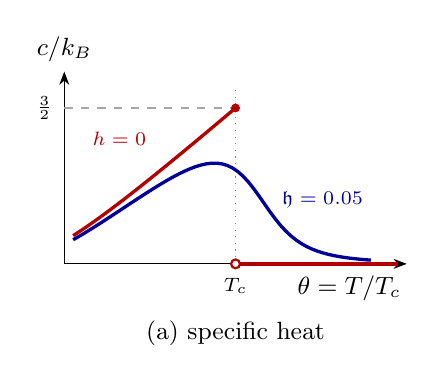
\begin{tikzpicture}[>=Stealth,font=\small,x=3.75cm,y=1.32cm]
  \draw[->] (0.42,0) -- (1.58,0);
  \node[anchor=north east,inner sep=2pt] at (1.58,-0.06) {$\theta=T/T_c$};
  \draw[->] (0.42,0) -- (0.42,1.85) node[above]{$c/k_B$};
  \draw[dotted,gray] (1,0) -- (1,1.70);
  \draw[dashed,gray!70] (0.42,1.5) -- (1.00,1.5);
  \node[anchor=east,font=\scriptsize,inner sep=2pt] at (0.40,1.5) {$\tfrac32$};
  \node[anchor=north,font=\scriptsize] at (1,-0.04) {$T_c$};
  \draw[very thick,red!70!black] plot coordinates{(0.4500,0.2717) (0.4620,0.2936) (0.4740,0.3159) (0.4860,0.3388) (0.4980,0.3620) (0.5100,0.3857) (0.5220,0.4097) (0.5340,0.4340) (0.5460,0.4587) (0.5580,0.4837) (0.5700,0.5089) (0.5820,0.5343) (0.5940,0.5600) (0.6060,0.5860) (0.6180,0.6121) (0.6300,0.6384) (0.6420,0.6649) (0.6540,0.6915) (0.6660,0.7183) (0.6780,0.7453) (0.6900,0.7724) (0.7020,0.7996) (0.7140,0.8269) (0.7260,0.8543) (0.7380,0.8819) (0.7500,0.9095) (0.7620,0.9372) (0.7740,0.9650) (0.7860,0.9929) (0.7980,1.0209) (0.8100,1.0489) (0.8220,1.0770) (0.8340,1.1052) (0.8460,1.1335) (0.8580,1.1617) (0.8700,1.1901) (0.8820,1.2185) (0.8940,1.2469) (0.9060,1.2754) (0.9180,1.3040) (0.9300,1.3326) (0.9420,1.3612) (0.9540,1.3898) (0.9660,1.4185) (0.9780,1.4473) (0.9900,1.4760)};
  \draw[very thick,red!70!black] (0.99,1.4760) -- (1.00,1.50);
  \draw[very thick,red!70!black] (1.00,0) -- (1.55,0);
  \fill[red!70!black] (1.00,1.50) circle (1.6pt);
  \draw[red!70!black,fill=white,thick] (1.00,0) circle (1.6pt);
  \draw[very thick,blue!60!black] plot coordinates{(0.4500,0.2320) (0.4680,0.2614) (0.4860,0.2918) (0.5040,0.3231) (0.5220,0.3550) (0.5400,0.3875) (0.5580,0.4205) (0.5760,0.4538) (0.5940,0.4874) (0.6120,0.5212) (0.6300,0.5550) (0.6480,0.5888) (0.6660,0.6224) (0.6840,0.6557) (0.7020,0.6886) (0.7200,0.7210) (0.7380,0.7526) (0.7560,0.7834) (0.7740,0.8131) (0.7920,0.8414) (0.8100,0.8681) (0.8280,0.8928) (0.8460,0.9150) (0.8640,0.9344) (0.8820,0.9502) (0.9000,0.9618) (0.9180,0.9683) (0.9360,0.9687) (0.9540,0.9620) (0.9720,0.9469) (0.9900,0.9224) (1.0080,0.8875) (1.0260,0.8419) (1.0440,0.7861) (1.0620,0.7215) (1.0800,0.6506) (1.0980,0.5768) (1.1160,0.5037) (1.1340,0.4346) (1.1520,0.3715) (1.1700,0.3159) (1.1880,0.2680) (1.2060,0.2273) (1.2240,0.1932) (1.2420,0.1648) (1.2600,0.1412) (1.2780,0.1216) (1.2960,0.1053) (1.3140,0.0916) (1.3320,0.0801) (1.3500,0.0705) (1.3680,0.0623) (1.3860,0.0553) (1.4040,0.0494) (1.4220,0.0442) (1.4400,0.0398) (1.4580,0.0360)};
  \node[anchor=west,font=\scriptsize,red!70!black,inner sep=1.5pt] at (0.50,1.20) {$h=0$};
  \node[anchor=west,font=\scriptsize,blue!60!black,inner sep=1.5pt] at (1.14,0.62) {$\mathfrak{h}=0.05$};
  \node[anchor=north,font=\small] at (1.0,-0.45) {(a) specific heat};
\end{tikzpicture}
\hfill
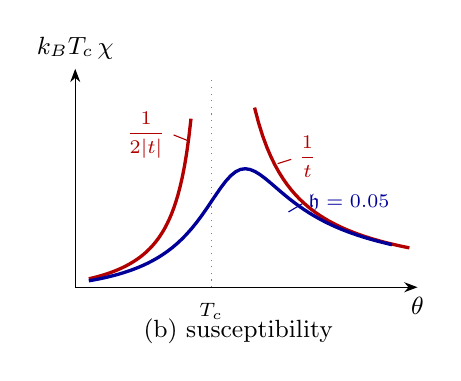
\begin{tikzpicture}[>=Stealth,font=\small,x=3.45cm,y=0.365cm]
  \draw[->] (0.50,0) -- (1.76,0) node[below]{$\theta$};
  \draw[->] (0.50,0) -- (0.50,7.60) node[above]{$k_BT_c\,\chi$};
  \draw[dotted,gray] (1,0) -- (1,7.35);
  \node[anchor=north,font=\scriptsize] at (1,-0.22) {$T_c$};
  \draw[very thick,red!70!black] plot coordinates{(0.5500,0.2935) (0.5580,0.3111) (0.5660,0.3295) (0.5740,0.3487) (0.5820,0.3688) (0.5900,0.3899) (0.5980,0.4119) (0.6060,0.4350) (0.6140,0.4592) (0.6220,0.4845) (0.6300,0.5111) (0.6380,0.5390) (0.6460,0.5683) (0.6540,0.5990) (0.6620,0.6314) (0.6700,0.6654) (0.6780,0.7013) (0.6860,0.7391) (0.6940,0.7791) (0.7020,0.8213) (0.7100,0.8659) (0.7180,0.9132) (0.7260,0.9635) (0.7340,1.0168) (0.7420,1.0736) (0.7500,1.1342) (0.7580,1.1988) (0.7660,1.2681) (0.7740,1.3423) (0.7820,1.4222) (0.7900,1.5082) (0.7980,1.6012) (0.8060,1.7020) (0.8140,1.8116) (0.8220,1.9312) (0.8300,2.0622) (0.8380,2.2063) (0.8460,2.3655) (0.8540,2.5422) (0.8620,2.7396) (0.8700,2.9615) (0.8780,3.2126) (0.8860,3.4992) (0.8940,3.8292) (0.9020,4.2132) (0.9100,4.6657) (0.9180,5.2067) (0.9260,5.8650)};
  \draw[very thick,red!70!black] plot coordinates{(1.1600,6.2500) (1.1750,5.7143) (1.1900,5.2632) (1.2050,4.8780) (1.2200,4.5455) (1.2350,4.2553) (1.2500,4.0000) (1.2650,3.7736) (1.2800,3.5714) (1.2950,3.3898) (1.3100,3.2258) (1.3250,3.0769) (1.3400,2.9412) (1.3550,2.8169) (1.3700,2.7027) (1.3850,2.5974) (1.4000,2.5000) (1.4150,2.4096) (1.4300,2.3256) (1.4450,2.2472) (1.4600,2.1739) (1.4750,2.1053) (1.4900,2.0408) (1.5050,1.9802) (1.5200,1.9231) (1.5350,1.8692) (1.5500,1.8182) (1.5650,1.7699) (1.5800,1.7241) (1.5950,1.6807) (1.6100,1.6393) (1.6250,1.6000) (1.6400,1.5625) (1.6550,1.5267) (1.6700,1.4925) (1.6850,1.4599) (1.7000,1.4286) (1.7150,1.3986) (1.7300,1.3699)};
  \draw[very thick,blue!60!black] plot coordinates{(0.5500,0.2239) (0.5680,0.2540) (0.5860,0.2869) (0.6040,0.3227) (0.6220,0.3617) (0.6400,0.4041) (0.6580,0.4504) (0.6760,0.5009) (0.6940,0.5561) (0.7120,0.6163) (0.7300,0.6823) (0.7480,0.7545) (0.7660,0.8339) (0.7840,0.9211) (0.8020,1.0172) (0.8200,1.1232) (0.8380,1.2403) (0.8560,1.3698) (0.8740,1.5130) (0.8920,1.6713) (0.9100,1.8460) (0.9280,2.0380) (0.9460,2.2477) (0.9640,2.4744) (0.9820,2.7157) (1.0000,2.9671) (1.0180,3.2208) (1.0360,3.4661) (1.0540,3.6897) (1.0720,3.8772) (1.0900,4.0162) (1.1080,4.0990) (1.1260,4.1242) (1.1440,4.0964) (1.1620,4.0248) (1.1800,3.9202) (1.1980,3.7933) (1.2160,3.6534) (1.2340,3.5076) (1.2520,3.3612) (1.2700,3.2176) (1.2880,3.0791) (1.3060,2.9471) (1.3240,2.8221) (1.3420,2.7044) (1.3600,2.5939) (1.3780,2.4904) (1.3960,2.3935) (1.4140,2.3028) (1.4320,2.2179) (1.4500,2.1383) (1.4680,2.0638) (1.4860,1.9938) (1.5040,1.9280) (1.5220,1.8662) (1.5400,1.8080) (1.5580,1.7531) (1.5760,1.7012) (1.5940,1.6523) (1.6120,1.6059) (1.6300,1.5620) (1.6480,1.5203) (1.6660,1.4807)};
  \node[anchor=east,font=\scriptsize,red!70!black,inner sep=2pt] at (0.855,5.30) {$\dfrac{1}{2|t|}$};
  \draw[red!70!black,thin] (0.862,5.30) -- (0.915,5.10);
  \node[anchor=west,font=\scriptsize,red!70!black,inner sep=2pt] at (1.30,4.55) {$\dfrac{1}{t}$};
  \draw[red!70!black,thin] (1.295,4.45) -- (1.245,4.30);
  \node[anchor=west,font=\scriptsize,blue!60!black,inner sep=1.5pt] at (1.34,2.95) {$\mathfrak{h}=0.05$};
  \draw[blue!60!black,thin] (1.335,2.90) -- (1.285,2.62);
  \node[anchor=north,font=\small] at (1.1,-0.75) {(b) susceptibility};
\end{tikzpicture}

\vspace{2ex}
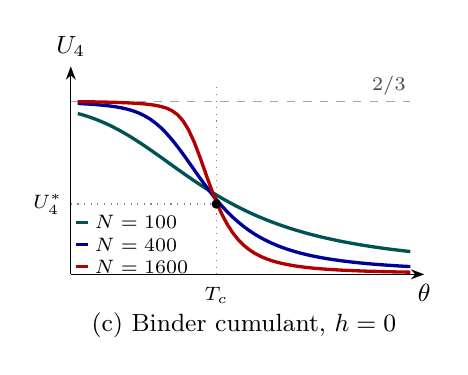
\begin{tikzpicture}[>=Stealth,font=\small,x=8.80cm,y=3.30cm]
  \draw[->] (0.79,0) -- (1.30,0) node[below]{$\theta$};
  \draw[->] (0.79,0) -- (0.79,0.80) node[above]{$U_4$};
  \draw[dashed,gray!70] (0.79,0.6667) -- (1.28,0.6667);
  \node[anchor=south east,font=\scriptsize,gray!55!black,inner sep=1.5pt] at (1.28,0.672) {$2/3$};
  \draw[dotted,gray] (1,0) -- (1,0.72);
  \draw[dotted,gray] (0.79,0.27052) -- (1.00,0.27052);
  \node[anchor=east,font=\scriptsize,inner sep=2pt] at (0.786,0.27052) {$U_4^{\ast}$};
  \node[anchor=north,font=\scriptsize] at (1,-0.012) {$T_c$};
  \draw[very thick,teal!65!black] plot coordinates{(0.8000,0.6190) (0.8080,0.6130) (0.8160,0.6062) (0.8240,0.5987) (0.8320,0.5903) (0.8400,0.5811) (0.8480,0.5711) (0.8560,0.5602) (0.8640,0.5486) (0.8720,0.5362) (0.8800,0.5231) (0.8880,0.5094) (0.8960,0.4953) (0.9040,0.4807) (0.9120,0.4657) (0.9200,0.4506) (0.9280,0.4353) (0.9360,0.4200) (0.9440,0.4048) (0.9520,0.3897) (0.9600,0.3748) (0.9680,0.3602) (0.9760,0.3459) (0.9840,0.3321) (0.9920,0.3186) (1.0000,0.3056) (1.0080,0.2930) (1.0160,0.2810) (1.0240,0.2694) (1.0320,0.2583) (1.0400,0.2477) (1.0480,0.2376) (1.0560,0.2279) (1.0640,0.2188) (1.0720,0.2100) (1.0800,0.2017) (1.0880,0.1938) (1.0960,0.1863) (1.1040,0.1792) (1.1120,0.1724) (1.1200,0.1660) (1.1280,0.1599) (1.1360,0.1541) (1.1440,0.1487) (1.1520,0.1434) (1.1600,0.1385) (1.1680,0.1338) (1.1760,0.1294) (1.1840,0.1251) (1.1920,0.1211) (1.2000,0.1173) (1.2080,0.1136) (1.2160,0.1101) (1.2240,0.1068) (1.2320,0.1037) (1.2400,0.1007) (1.2480,0.0978) (1.2560,0.0951) (1.2640,0.0925) (1.2720,0.0900) (1.2800,0.0876)};
  \draw[very thick,blue!60!black] plot coordinates{(0.8000,0.6575) (0.8080,0.6564) (0.8160,0.6552) (0.8240,0.6537) (0.8320,0.6519) (0.8400,0.6498) (0.8480,0.6473) (0.8560,0.6442) (0.8640,0.6402) (0.8720,0.6353) (0.8800,0.6290) (0.8880,0.6210) (0.8960,0.6109) (0.9040,0.5983) (0.9120,0.5828) (0.9200,0.5644) (0.9280,0.5428) (0.9360,0.5184) (0.9440,0.4915) (0.9520,0.4628) (0.9600,0.4328) (0.9680,0.4023) (0.9760,0.3721) (0.9840,0.3426) (0.9920,0.3144) (1.0000,0.2878) (1.0080,0.2631) (1.0160,0.2402) (1.0240,0.2193) (1.0320,0.2003) (1.0400,0.1831) (1.0480,0.1676) (1.0560,0.1537) (1.0640,0.1412) (1.0720,0.1299) (1.0800,0.1198) (1.0880,0.1108) (1.0960,0.1026) (1.1040,0.0953) (1.1120,0.0887) (1.1200,0.0827) (1.1280,0.0773) (1.1360,0.0724) (1.1440,0.0680) (1.1520,0.0639) (1.1600,0.0602) (1.1680,0.0569) (1.1760,0.0538) (1.1840,0.0510) (1.1920,0.0484) (1.2000,0.0460) (1.2080,0.0438) (1.2160,0.0417) (1.2240,0.0399) (1.2320,0.0381) (1.2400,0.0365) (1.2480,0.0350) (1.2560,0.0336) (1.2640,0.0322) (1.2720,0.0310) (1.2800,0.0299)};
  \draw[very thick,red!70!black] plot coordinates{(0.8000,0.6645) (0.8080,0.6642) (0.8160,0.6640) (0.8240,0.6636) (0.8320,0.6633) (0.8400,0.6628) (0.8480,0.6623) (0.8560,0.6617) (0.8640,0.6609) (0.8720,0.6600) (0.8800,0.6589) (0.8880,0.6576) (0.8960,0.6558) (0.9040,0.6535) (0.9120,0.6504) (0.9200,0.6460) (0.9280,0.6397) (0.9360,0.6299) (0.9440,0.6145) (0.9520,0.5907) (0.9600,0.5558) (0.9680,0.5095) (0.9760,0.4538) (0.9840,0.3935) (0.9920,0.3339) (1.0000,0.2791) (1.0080,0.2314) (1.0160,0.1914) (1.0240,0.1587) (1.0320,0.1322) (1.0400,0.1110) (1.0480,0.0939) (1.0560,0.0802) (1.0640,0.0691) (1.0720,0.0600) (1.0800,0.0525) (1.0880,0.0463) (1.0960,0.0411) (1.1040,0.0368) (1.1120,0.0331) (1.1200,0.0299) (1.1280,0.0272) (1.1360,0.0249) (1.1440,0.0228) (1.1520,0.0211) (1.1600,0.0195) (1.1680,0.0181) (1.1760,0.0169) (1.1840,0.0157) (1.1920,0.0148) (1.2000,0.0139) (1.2080,0.0131) (1.2160,0.0123) (1.2240,0.0117) (1.2320,0.0111) (1.2400,0.0105) (1.2480,0.0100) (1.2560,0.0095) (1.2640,0.0091) (1.2720,0.0087) (1.2800,0.0083)};
  \fill (1.0,0.27052) circle (1.7pt);
  \draw[very thick,teal!65!black] (0.797,0.200) -- (0.815,0.200);
  \node[anchor=west,font=\scriptsize,inner sep=1.5pt] at (0.818,0.200) {$N=100$};
  \draw[very thick,blue!60!black] (0.797,0.115) -- (0.815,0.115);
  \node[anchor=west,font=\scriptsize,inner sep=1.5pt] at (0.818,0.115) {$N=400$};
  \draw[very thick,red!70!black] (0.797,0.030) -- (0.815,0.030);
  \node[anchor=west,font=\scriptsize,inner sep=1.5pt] at (0.818,0.030) {$N=1600$};
  \node[anchor=north,font=\small] at (1.04,-0.11) {(c) Binder cumulant, $h=0$};
\end{tikzpicture}
\caption{Response functions and Binder cumulant of the mean-field Ising model,
computed exactly. \textbf{(a)} At $h=0$ the specific heat rises to
$\tfrac32k_B$ at $T_c^{-}$ and is identically zero above (open circle): a finite
\emph{jump}, i.e.\ $\alpha=0$ without divergence. A field $\mathfrak{h}=0.05$
rounds the jump into a smooth bounded peak displaced above $T_c$, and makes $c$
nonzero above $T_c$ because $m\neq0$ there. \textbf{(b)} At $h=0$ the
susceptibility diverges from both sides as $|t|^{-1}$ (curves truncated at the top
of the frame), with amplitudes in the ratio $C_+/C_-=2$; the field cuts the
divergence off at $|t|\sim\mathfrak{h}^{2/3}$ and leaves a finite maximum.
\textbf{(c)} $U_4$ from the exact finite-$N$ Curie--Weiss sums. The curves tend to
$0$ above $T_c$ and to $2/3$ below, and pass through the universal value
$U_4^{\ast}=0.270520$ at $T_c$ --- the mean-field Binder crossing of
Section~\ref{sec:fss:observables}. The residual spread at $T_c$ ($0.3056$,
$0.2878$, $0.2791$ for the three sizes) is the corrections-to-scaling drift of
Section~\ref{sec:fss:corrections}, here decaying as $N^{-1/2}$.}
\label{fig:appising2}
\end{figure}


\section{Worked example: the mean-field \texorpdfstring{$q$}{q}-state Potts model}
\label{sec:apppotts}

Appendix~\ref{sec:appising} ended by observing what the Ising model cannot supply:
a bimodal $P(E)$, because its two coexisting phases are symmetry images and
therefore share an energy density. The $q$-state Potts model with $q>2$ repairs
exactly that deficiency, and it does so in the cleanest possible way --- the
ordered and disordered phases are \emph{not} related by any symmetry, so they
differ in energy, and mean-field theory delivers a genuine temperature-driven
first-order transition whose transition temperature, order-parameter jump and
latent heat are all available in \emph{closed form}. This appendix computes the
same list of quantities as Appendix~\ref{sec:appising}, in the same order, so the
two can be read side by side.

\subsection{The model and the decoupling}
\label{sec:apppotts:model}

Place a $q$-valued variable $\sigma_i\in\{1,\dots,q\}$ on each of $N$ sites with
$z$ neighbours, and reward agreement:
\[
\hat H=-J\sum_{\langle ij\rangle}\delta_{\sigma_i\sigma_j} ,\qquad J>0 .
\]
For $q=2$ this is the Ising model: $\delta_{\sigma\sigma'}=\tfrac12(1+ss')$ with
$s=\pm1$, so $J_{\rm Potts}=2J_{\rm Ising}$ up to an additive constant --- a
mapping used as a check throughout.

To decouple, resolve the Kronecker delta into occupation variables. Put
$n_i^{a}\equiv\delta_{\sigma_i,a}$, so that $\sum_a n_i^{a}=1$ identically, and
let
\[
x_a\equiv\langle n_i^{a}\rangle=\frac{N_a}{N},\qquad \sum_{a=1}^{q}x_a=1 ,
\]
be the fraction of sites in state $a$. Then
$\delta_{\sigma_i\sigma_j}=\sum_a n_i^{a}n_j^{a}$, and the mean-field step is the
same one as in Section~\ref{sec:appising:model} applied to each species,
\[
n_i^{a}n_j^{a}\;\approx\;x_a n_i^{a}+x_a n_j^{a}-x_a^{2} ,
\]
dropping $\langle\delta n_i^a\,\delta n_j^a\rangle$. With
$\sum_{\langle ij\rangle}1=Nz/2$ and $\sum_{\langle ij\rangle}(n_i^a+n_j^a)=z\sum_i
n_i^a$,
\[
\hat H_{\rm MF}=\frac{NzJ}{2}\sum_a x_a^{2}\;-\;zJ\sum_i\sum_a x_a\,n_i^{a} ,
\]
so each site sees a field $zJx_a$ favouring state $a$; the sites are independent
and
\[
\boxed{\;
f(\{x_a\})=\frac{zJ}{2}\sum_a x_a^{2}
-k_BT\,\ln\!\sum_{a=1}^{q}e^{\beta zJ x_a}\;}
\]
Stationarity of $f$ subject to $\sum_ax_a=1$ gives the self-consistency condition
\[
x_a=\frac{e^{\beta zJ x_a}}{\sum_b e^{\beta zJ x_b}} .
\]

\paragraph{One order parameter suffices.} The disordered solution is
$x_a=1/q$ for all $a$. An ordered solution singles out one state --- say $a=1$ ---
and treats the rest symmetrically, which is a one-parameter family:
\[
\boxed{\;
x_1=\frac{1+(q-1)m}{q},\qquad
x_{a}=\frac{1-m}{q}\ \ (a=2,\dots,q)\;}
\]
Here $m=x_1-x_2$ is the excess concentration of the favoured state, equivalently
$m=(qx_1-1)/(q-1)$; it runs over
\[
-\frac{1}{q-1}\;\leq\;m\;\leq\;1 ,
\]
with $m=0$ disordered, $m=1$ fully ordered, and $m<0$ meaning state $1$ is
\emph{depleted}. Note at once the structural difference from Ising: the range is
\emph{not} symmetric about zero unless $q=2$. That asymmetry is the whole
difference between a second- and a first-order transition, as
Section~\ref{sec:apppotts:landau} makes precise.

Substituting the parametrisation and using $\sum_a x_a^2=[1+(q-1)m^2]/q$ (a
one-line expansion) together with $x_1-x_a=m$, the self-consistency condition
collapses to a single scalar equation,
\[
\boxed{\;
\frac{1+(q-1)m}{1-m}=e^{\tilde\beta m},
\qquad\text{equivalently}\qquad
m=\frac{e^{\tilde\beta m}-1}{e^{\tilde\beta m}+q-1},
\qquad \tilde\beta\equiv\frac{zJ}{k_BT}\;}
\]
For $q=2$ this is $m=\tanh(\tilde\beta m/2)$, which with $J_{\rm
Potts}=2J_{\rm Ising}$ is $m=\tanh(m/\theta)$ --- the Weiss equation of
Section~\ref{sec:appising:model}, as required.

\subsection{The exact constrained free energy}
\label{sec:apppotts:exact}

As in Section~\ref{sec:appising:exact}, the decoupling is \emph{exact} for the
fully-connected version, and there the constrained free energy can be written
down without approximation. Take
\[
\hat H=-\frac{\tilde J}{2N}\sum_{a}N_a^{2}+\text{const},
\qquad \tilde J\equiv zJ ,
\]
which is the fully-connected form of the same model (it counts every pair of
like-valued sites with weight $\tilde J/N$). Since $\hat H$ depends on the
configuration only through the occupation numbers $\{N_a\}$, the constrained trace
is again a counting problem --- now multinomial rather than binomial:
\[
e^{-\beta N f_N}
=\Tr\Big[\textstyle\prod_a\delta(\hat N_a-N_a)\,e^{-\beta\hat H}\Big]
=\frac{N!}{\prod_a N_a!}\;
\exp\!\Big[\beta N\,\frac{\tilde J}{2}\sum_a x_a^{2}\Big] ,
\]
and Stirling gives $\ln(N!/\prod_aN_a!)=N\mathfrak{s}(\{x\})+O(\ln N)$ with
$\mathfrak{s}=-\sum_ax_a\ln x_a$. Hence, exactly,
\[
\boxed{\;
f_N(\{x_a\})=-\frac{\tilde J}{2}\sum_a x_a^{2}
+k_BT\sum_a x_a\ln x_a ,
\qquad
P_N(\{x_a\})\propto e^{-\beta N f_N}\;}
\]
Restricted to the one-parameter family above, with
$\sum_ax_a^{2}=[1+(q-1)m^{2}]/q$ and
$\mathfrak{s}=\ln q-G(m)/q$ where
\[
\boxed{\;
G(m)\equiv\big[1+(q-1)m\big]\ln\!\big[1+(q-1)m\big]+(q-1)(1-m)\ln(1-m)\;}
\]
this becomes a function of the single variable $m$:
\[
\boxed{\;
\Delta f(m)\equiv f_N(m)-f_N(0)
=-\frac{\tilde J(q-1)}{2q}\,m^{2}\;+\;\frac{k_BT}{q}\,G(m)\;}
\]
with $G(0)=G'(0)=0$. Two facts are recorded for use below: the energy and entropy
densities are
\[
\boxed{\;
u(m)=-\frac{\tilde J}{2q}\big[1+(q-1)m^{2}\big],
\qquad
s(m)=k_B\Big[\ln q-\frac{G(m)}{q}\Big]\;}
\]
Setting $\Delta f'(m)=0$ returns
$\ln\frac{1+(q-1)m}{1-m}=\tilde\beta m$, the self-consistency equation of
Section~\ref{sec:apppotts:model}, confirming that the two routes agree. So once
again the mean-field free energy \emph{is} the exact constrained free energy of
Section~\ref{sec:minimum}, and $P_N(m)$ is known rather than modelled.

\paragraph{The state space is a simplex, not a line.} One difference from the
Ising case must be kept in view. The full order-parameter space is the
$(q-1)$-dimensional simplex $\{x_a\geq0,\sum_ax_a=1\}$, and the $m$-parametrisation
is a \emph{ray} in it: the segment from the centroid $x_a=1/q$ towards the vertex
$x_1=1$. Because the Hamiltonian is symmetric under permuting the $q$ states,
there are $q$ such equivalent rays, and every ordered stationary point found below
comes in $q$ copies. Mapping the simplex to the plane by
$\mathbf{X}=\sum_ax_a\mathbf{V}_a$ with the $\mathbf{V}_a$ the vertices of a
regular simplex centred at the origin, the parametrisation becomes simply
$\mathbf{X}=m\,\mathbf{V}_1$: the order parameter $m$ is the fractional distance
from the centre towards a vertex. Figure~\ref{fig:apppotts1}c uses this for $q=3$.

\subsection{Landau expansion: the cubic term is the whole story}
\label{sec:apppotts:landau}

Expand $G$. From $G'(m)=(q-1)\big[\ln(1+(q-1)m)-\ln(1-m)\big]$ one gets
\[
G''(0)=q(q-1),\qquad
G'''(0)=q(q-1)(2-q),\qquad
G''''(0)=2(q-1)\big[(q-1)^{3}+1\big],
\]
so that
\[
\boxed{\;
\begin{aligned}
\Delta f(m)=\;&\frac{q-1}{2}\Big(k_BT-\frac{\tilde J}{q}\Big)m^{2}
\;-\;\frac{k_BT\,(q-1)(q-2)}{6}\,m^{3}\\[2pt]
&+\;\frac{k_BT\,(q-1)\big[(q-1)^{3}+1\big]}{12\,q}\,m^{4}\;+\;O(m^{5})
\end{aligned}\;}
\]
Everything follows from the middle term.

\paragraph{$q=2$: no cubic term, second order.} At $q=2$ the cubic coefficient
$\propto(q-2)$ vanishes identically --- as it must, since $\mathbb{Z}_2$ symmetry
forbids odd powers --- and the expansion reduces to
$\Delta f=\tfrac12(k_BT-\tilde J/2)m^{2}+\tfrac{k_BT}{12}m^{4}$. With
$\tilde J_{\rm Potts}=2\tilde J_{\rm Ising}=2k_BT_c$ this is exactly the Ising
Landau form of Section~\ref{sec:appising:landau}, $a=k_BT_c$ and
$b=k_BT/3$ (note $b/4=k_BT/12$), and the transition is continuous.

\paragraph{$q>2$: a cubic term, hence first order.} For $q>2$ the cubic
coefficient is strictly negative, and a cubic term changes the character of the
transition completely. Write $\Delta f=Am^{2}+Bm^{3}+Cm^{4}$ with
\[
A=\frac{q-1}{2}\big(k_BT-k_BT_0\big),\quad
k_BT_0\equiv\frac{\tilde J}{q},\qquad
B=-\frac{k_BT(q-1)(q-2)}{6}<0,\qquad
C>0 .
\]
Because $B\neq0$, a \emph{second minimum at $m>0$ appears while $A$ is still
positive} --- that is, while $m=0$ is still a perfectly good local minimum. The
two minima exchange stability at the temperature where they are degenerate, which
is the condition
\[
\Delta f(m)=m^{2}\big(A+Bm+Cm^{2}\big)=0\ \text{with a double root},
\]
i.e.\ $B^{2}=4AC$, giving
\[
A_t=\frac{B^{2}}{4C},\qquad m_t=-\frac{B}{2C} ,
\]
at which point $\Delta f=C\,m^{2}(m-m_t)^{2}\geq0$ with equality at $m=0$ and
$m=m_t$: two degenerate minima separated by a barrier. That is a first-order
transition, and it occurs at $A_t>0$, hence at
\[
T_t>T_0 .
\]
So $T_0$, the temperature at which the disordered state loses local stability, is
\emph{not} the transition temperature when $q>2$; it is a spinodal lying below it
(Section~\ref{sec:apppotts:spinodal}). The whole first-order structure ---
two minima, a barrier, metastability, a latent heat --- is generated by the
single term $Bm^{3}$, which exists because the $q$ states can be ordered in one
way and disordered in another, with nothing relating the two.

\subsection{The transition, in closed form}
\label{sec:apppotts:transition}

The Landau truncation locates the transition only approximately, but for this
model the \emph{exact} answer is available, and it is remarkably simple. The
transition is fixed by two conditions on the exact $\Delta f$: the ordered
minimum must be stationary and degenerate with the disordered one,
\begin{align*}
\text{(i)}\quad \Delta f'(m_t)&=0
&&\Longleftrightarrow&&
\ln\frac{1+(q-1)m_t}{1-m_t}=\tilde\beta_t m_t ,\\
\text{(ii)}\quad \Delta f(m_t)&=0
&&\Longleftrightarrow&&
G(m_t)=\frac{\tilde\beta_t(q-1)}{2}m_t^{2} .
\end{align*}
Both are satisfied exactly by
\[
\boxed{\;
m_t=\frac{q-2}{q-1},
\qquad
k_BT_t=\frac{\tilde J}{2}\,\frac{q-2}{(q-1)\ln(q-1)},
\qquad
\tilde\beta_t=\frac{2(q-1)\ln(q-1)}{q-2}\;}
\]
The verification is worth doing because it is two lines. With
$m_t=(q-2)/(q-1)$,
\[
1+(q-1)m_t=q-1,\qquad 1-m_t=\frac{1}{q-1},
\qquad\text{so}\qquad
\frac{1+(q-1)m_t}{1-m_t}=(q-1)^{2} ,
\]
and (i) reads $(q-1)^{2}=e^{\tilde\beta_tm_t}$, i.e.\
$\tilde\beta_tm_t=2\ln(q-1)$, which is the boxed $\tilde\beta_t$. For (ii),
\[
G(m_t)=(q-1)\ln(q-1)+(q-1)\cdot\frac{1}{q-1}\cdot\ln\frac{1}{q-1}
=(q-2)\ln(q-1) ,
\]
while the right-hand side is
$\tfrac12\cdot\tfrac{2(q-1)\ln(q-1)}{q-2}\cdot(q-1)\cdot\tfrac{(q-2)^{2}}{(q-1)^{2}}
=(q-2)\ln(q-1)$. They agree identically.

\paragraph{The $q\to2$ limit.} As $q\to2^{+}$ one has $m_t\to0$ and, using
$\ln(q-1)\simeq(q-2)$, $k_BT_t\to\tilde J/2=\tilde J_{\rm Ising}=k_BT_c$: the
order-parameter jump closes continuously and the transition temperature merges
with $T_0=\tilde J/q=\tilde J/2$. The first-order transition degenerates
continuously into the Ising second-order one at $q=2$, exactly as it should.

\paragraph{Latent heat.} Because the two phases have equal free energy at $T_t$,
the energy difference \emph{is} the latent heat, $L=T_t\Delta S=\Delta u$. From
$u(m)$,
\[
\boxed{\;
L=u(0)-u(m_t)=\frac{\tilde J(q-1)}{2q}m_t^{2}
=\frac{\tilde J}{2}\,\frac{(q-2)^{2}}{q(q-1)}\;}
\]
and independently, from the entropy,
\[
\boxed{\;
\Delta S=s(0)-s(m_t)=k_B\frac{G(m_t)}{q}=k_B\,\frac{(q-2)\ln(q-1)}{q}\;}
\]
The two are consistent: $T_t\Delta S = \frac{\tilde J(q-2)}{2(q-1)\ln(q-1)}\cdot
\frac{(q-2)\ln(q-1)}{q}=\frac{\tilde J(q-2)^{2}}{2q(q-1)}=L$ \checkmark. Both
vanish $\propto(q-2)^{2}$ and $\propto(q-2)$ respectively as $q\to2$, which is the
statement that the Ising transition has no latent heat
(Section~\ref{sec:appising:caseB}).

This is the quantity Appendix~\ref{sec:appising} could not produce, and everything
distinctive below follows from it being nonzero.

\subsection{Spinodals and metastability}
\label{sec:apppotts:spinodal}

Two spinodals bracket the transition, and unlike the Ising case at $h=0$ they are
at \emph{different} temperatures from $T_t$, so there is a genuine metastability
window.

\paragraph{Lower (disordered) spinodal.} The disordered minimum $m=0$ survives as
a local minimum while $\Delta f''(0)>0$. From the expansion,
$\Delta f''(0)=(q-1)(k_BT-\tilde J/q)$, so
\[
\boxed{\;k_BT_0=\frac{\tilde J}{q}\;}
\]
Below $T_0$ the disordered state is not merely metastable but locally unstable, and
for $T_0<T<T_t$ it is metastable. At $q=2$, $k_BT_0=\tilde J/2=k_BT_t$ and the
window closes.

\paragraph{Upper (ordered) spinodal.} The ordered minimum disappears where it
merges with the intervening maximum, $\Delta f'=\Delta f''=0$. Using
\[
\Delta f''(m)=\frac{k_BT(q-1)}{q}\,D(m),
\qquad
\boxed{\;D(m)\equiv\frac{q-1}{1+(q-1)m}+\frac{1}{1-m}-\tilde\beta\;}
\]
this is the pair $\tilde\beta=\frac{q-1}{1+(q-1)m}+\frac{1}{1-m}$ and
$\tilde\beta m=\ln\frac{1+(q-1)m}{1-m}$, which has no closed-form solution but is
a one-line numerical root. Table~\ref{tab:apppotts} lists $T_1$; always
$T_0<T_t<T_1$.

\paragraph{How wide is the window?} For $q=3$ it is narrow --- $T_0/T_t=0.9244$,
$T_1/T_t=1.0098$ --- and for $q=10$ it is wide, $T_0/T_t=0.4944$,
$T_1/T_t=1.0842$. The narrowness at $q=3$ is one face of a general fact: the
mean-field $q=3$ transition is \emph{weakly} first order. Its latent heat is
$L=\tilde J/12$ and, more tellingly, the free-energy barrier at $T_t$ is only
$\Delta f_b=1.1\times10^{-3}\,k_BT_t$, against $7.1\times10^{-2}\,k_BT_t$ at
$q=10$. Section~\ref{sec:apppotts:distributions} shows what that does to the
observability of the transition, and it is exactly the difficulty flagged at the
end of Section~\ref{sec:fss:firstorder}.

\subsection{Specific heat}
\label{sec:apppotts:c}

Differentiate $u(m)=-\frac{\tilde J}{2q}[1+(q-1)m^{2}]$ along a branch. Implicit
differentiation of the self-consistency equation gives
$dm/d\tilde\beta=m/D(m)$ and, with $\tilde\beta=\tilde J/k_BT$,
\[
\frac{dm}{dT}=-\frac{m\,\tilde\beta}{T\,D(m)} ,
\]
so that $c=du/dT=-\frac{\tilde J(q-1)}{q}m\frac{dm}{dT}$ becomes the exact
expression
\[
\boxed{\;
\frac{c}{k_B}=\frac{(q-1)\,\tilde\beta^{2}m^{2}}{q\,D(m)}\;}
\]
(positive on any branch that is a genuine minimum, where $D>0$). Reading it off:

\begin{itemize}
\item \textbf{$T>T_t$ (disordered):} $m=0$, hence $c=0$ identically. As in the
Ising case, mean-field theory gives a paramagnet no specific heat at all, because
with no correlations there is no way to absorb energy without ordering.
\item \textbf{$T\to T_t^{-}$ (ordered):} substituting $m=m_t$ and using
$1+(q-1)m_t=q-1$, $1-m_t=1/(q-1)$ gives the pleasantly simple
\[
\boxed{\;D_t\equiv D(m_t)=1+(q-1)-\tilde\beta_t=q-\tilde\beta_t\;}
\qquad\Longrightarrow\qquad
\frac{c(T_t^{-})}{k_B}=\frac{(q-1)\,\tilde\beta_t^{2}\,m_t^{2}}{q\,(q-\tilde\beta_t)} ,
\]
a finite number, e.g.\ $5.634$ for $q=3$ and $3.437$ for $q=10$.
\end{itemize}
So $c$ has a finite \emph{jump} at $T_t$, as at any first-order transition ---
\emph{plus}, and this is the part the smooth branches do not show, a delta
function carrying the latent heat:
\[
\boxed{\;
c(T)=c_{\rm branch}(T)+L\,\delta(T-T_t)\;}
\]
At finite $N$ the delta function is not a distribution but a peak, and its shape
is exactly the two-state result of Section~\ref{sec:fss:firstorder}: height
$\propto N$, width $\propto 1/N$, area $L$. The mean-field Potts model therefore
realises the entire first-order column of the discriminant table in that section,
with every entry computable.

Per unit volume the numbers above are divided by $a^{d}$, as in
Section~\ref{sec:appising:caseA}.

\subsection{Susceptibility}
\label{sec:apppotts:chi}

A field conjugate to the order parameter is obtained by favouring one state,
$\hat H\to\hat H-h\sum_i\delta_{\sigma_i,1}$, which contributes $-hx_1=
-h/q-\frac{h(q-1)}{q}m$ per site. So the field conjugate to $m$ itself is
$\tilde h\equiv h(q-1)/q$, and $\Delta f\to\Delta f-\tilde h m$. Then
$\chi\equiv(\partial m/\partial\tilde h)_T=1/\Delta f''(m)$, i.e.
\[
\boxed{\;
\chi=\frac{q}{k_BT\,(q-1)\,D(m)}\;}
\]
This single formula covers both branches, and it has three features worth
separating.

\paragraph{Above $T_t$: Curie--Weiss, but pointing at the spinodal.} With $m=0$,
$D(0)=q-\tilde\beta=q(T-T_0)/T$, so
\[
\boxed{\;
\chi_{\rm dis}=\frac{1}{k_B(q-1)\,(T-T_0)}\;}
\]
--- a Curie--Weiss law with $T_0$, \emph{not} $T_t$, in the denominator. At $q=2$
this is $\chi=1/[k_B(T-T_c)]$, exactly the Ising result of
Section~\ref{sec:appising:caseA}. For $q>2$ the divergence sits at $T_0<T_t$ and
is therefore \emph{never reached}: the transition pre-empts it. This is the
precise sense in which a first-order transition has no critical fluctuations ---
the divergence exists in the analytic continuation of the disordered branch, on
which the system stops sitting before getting there.

\paragraph{At $T_t$: finite, and in this model even continuous.} Since
$D(0)=q-\tilde\beta$ and $D(m_t)=q-\tilde\beta$ coincide --- the two terms of $D$
simply exchange values, because $1+(q-1)m_t=q-1$ and $1-m_t=1/(q-1)$ --- the
susceptibility takes the \emph{same} value on both sides:
\[
\boxed{\;
\chi(T_t^{-})=\chi(T_t^{+})=\frac{q}{k_BT_t(q-1)(q-\tilde\beta_t)}\;}
\]
For $q=10$ this is $0.2198/k_BT_t$. So $\chi$ is finite and continuous through a
first-order transition here, while its \emph{derivative} is not: the two branches
are different functions that happen to agree at $T_t$. Compare the Ising case,
where $\chi$ diverges as $|t|^{-1}$ from both sides with a universal amplitude
ratio of $2$; nothing of the sort survives when the transition is first order.

\paragraph{On the metastable branches: divergence at the spinodals.} Continued
below $T_t$, $\chi_{\rm dis}$ diverges as $(T-T_0)^{-1}$ at the lower spinodal;
continued above $T_t$, the ordered branch has $D(m)\to0$ at $T_1$ and $\chi$
diverges there too. Both divergences are on metastable branches and are therefore
mean-field artefacts in any finite dimension --- the caveat recorded in
footnote~\ref{fn:spinodal}. Figure~\ref{fig:apppotts2}c shows the full picture.

\subsection{The distributions: \texorpdfstring{$P(m)$}{P(m)} is \texorpdfstring{$(q{+}1)$}{(q+1)}-modal, \texorpdfstring{$P(E)$}{P(E)} is bimodal}
\label{sec:apppotts:distributions}

This is the payoff, and it is the entry of the table in
Section~\ref{sec:firstorder} that Appendix~\ref{sec:appising} could not reach.
Since $P_N\propto e^{-\beta Nf_N}$ exactly, one need only count the minima of
$f_N$ and read off their energies.

\paragraph{$P(\boldsymbol{\phi})$: exactly $q+1$ peaks at $T_t$.} On the
simplex, $f_N$ has:
\begin{itemize}
\item one stationary point at the centroid ($m=0$), the disordered state, a local
minimum for $T>T_0$;
\item $q$ equivalent stationary points at $m=m_t^{\rm(loc)}$ along each of the $q$
rays towards a vertex, local minima for $T<T_1$;
\end{itemize}
so for $T_0<T<T_1$ there are $q+1$ local minima, and at $T=T_t$ they are
\emph{all degenerate}, since that is what $\Delta f(m_t)=0$ says. Therefore
\[
\boxed{\;T=T_t:\qquad P(\boldsymbol{\phi})\ \text{has exactly }q+1\ \text{peaks:}\ q\ \text{ordered}+1\ \text{at}\ \boldsymbol{\phi}=0\;}
\]
which is precisely the row ``$q$-state Potts, first order, $T=T_t$:
$(q{+}1)$-modal'' of Section~\ref{sec:firstorder}, and precisely what
Figure~\ref{fig:histograms}d drew for $q=3$. Figure~\ref{fig:apppotts1}c
reproduces that picture from the actual $f_N$, with the four maxima at the
centroid and at $m_t=\tfrac12$ of the way to each vertex.

Off $T_t$ the count is unchanged but the peaks are no longer degenerate: for
$T>T_t$ the disordered peak dominates and the $q$ ordered ones are suppressed by
$e^{-\beta N|\Delta f|}$, for $T<T_t$ the reverse. As in
Section~\ref{sec:appising:caseB}, the multi-peak structure with comparable
weights exists only in a window of width $\Delta T\sim1/N$ about $T_t$ --- and
that window is exactly the rounding region of
Section~\ref{sec:fss:firstorder}, $\Delta T\sim L^{-d}$.

\paragraph{$P(E)$: exactly two peaks.} The energy density $u(m)$ depends on $m$
only through $m^{2}$ and is therefore the \emph{same} for all $q$ ordered states
--- they are permutations of one another. So the $q+1$ order-parameter peaks
collapse onto just \emph{two} energies,
\[
\boxed{\;
e_d=-\frac{\tilde J}{2q},
\qquad
e_o=-\frac{\tilde J}{2q}\big[1+(q-1)m_t^{2}\big]
=-\frac{\tilde J}{2q}\cdot\frac{q^{2}-3q+3}{q-1},
\qquad e_d-e_o=L\;}
\]
and $P(E)$ is bimodal with the two peaks separated by the latent heat. Explicitly,
integrating out the directions of the simplex at fixed $e$ leaves
\[
P(e)\;\propto\;e^{N[s_{\max}(e)/k_B-\beta e]}
=e^{-\beta N f_N(m_+(e))} ,
\]
where $m_+(e)>0$ is the entropy-maximising configuration at energy $e$ (one may
check that the maximiser has at most two distinct $x_a$, so the
$m$-parametrisation captures it, and that the $m>0$ branch is the one with the
larger entropy). At $T=T_t$ the exponent vanishes at both $e_d$ and $e_o$, giving
two peaks of \emph{equal} height --- coexistence
(Figure~\ref{fig:apppotts1}d).

So the contrast with Ising is complete and its origin is transparent:
\begin{center}
\renewcommand{\arraystretch}{1.2}
\begin{tabular}{@{}lll@{}}
\toprule
 & $P(\boldsymbol{\phi})$ & $P(E)$\\
\midrule
Ising, $T<T_c$, $h=0$ & $2$ peaks ($\pm m_s$) & \textbf{1} peak: the phases are
$\mathbb{Z}_2$ images\\
Potts $q>2$, $T=T_t$ & $q{+}1$ peaks & \textbf{2} peaks: ordered and disordered
are unrelated\\
\bottomrule
\end{tabular}
\end{center}
Bimodal $P(E)$ requires coexisting phases of \emph{different} energy density, and
symmetry-related phases never qualify. That is the general statement; the Potts
model is the minimal model exhibiting it.

\paragraph{Weak versus strong: why $q=3$ is hard.} The depth of the dip between
the peaks is set by the barrier, $P_{\min}/P_{\max}=e^{-\beta N\Delta f_b}$, and
$\Delta f_b/k_BT_t$ is $1.1\times10^{-3}$ at $q=3$ against
$7.1\times10^{-2}$ at $q=10$ (Table~\ref{tab:apppotts}). At $N=200$ that is a
peak-to-dip ratio of $1.3$ for $q=3$ and $1.6\times10^{6}$ for $q=10$: the same
transition, of the same order, is either invisible or unmistakable depending on
$q$. Figure~\ref{fig:apppotts1}b shows both at the same $N$. A simulation of the
$q=3$ model at that size would report a smooth unimodal histogram and conclude
``continuous''. This is the concrete content of the warning closing
Section~\ref{sec:fss:firstorder}: for a weak first-order transition, no analysis of
data with $L\lesssim\xi$ can identify the order, and the only cure is larger $L$.

\subsection{Binder cumulants}
\label{sec:apppotts:binder}

\paragraph{The energy cumulant, in closed form.} For a temperature-driven
first-order transition the natural diagnostic is the Challa--Landau--Binder energy
cumulant of Section~\ref{sec:fss:firstorder}, because it needs no symmetry and no
order parameter. Its two-state value was derived there; here both energies are
known, so it becomes an explicit prediction. With
$r\equiv e_o/e_d=1+(q-1)m_t^{2}=(q^{2}-3q+3)/(q-1)$,
\[
\boxed{\;
V_L^{\min}=\frac{2}{3}-\frac{1}{12}\left(r-\frac1r\right)^{2},
\qquad r=\frac{q^{2}-3q+3}{q-1}\;}
\]
which gives $0.6088$ at $q=3$, $0.3643$ at $q=4$, and $-4.650$ at $q=10$: a
deviation from $2/3$ that grows rapidly with $q$, exactly tracking the latent
heat. At $q=2$, $r=1$ and $V_L^{\min}=2/3$ --- no latent heat, no signal, which is
the Ising result.

\begin{warning}
$V_L$ is \emph{not} invariant under shifting the zero of energy, since it is built
from raw rather than central moments: $E\to E+{\rm const}$ changes $r$ and hence
the predicted value. The formula above uses the natural zero of the Potts
Hamiltonian as written, $\hat H=-J\sum\delta_{\sigma\sigma'}$, and a numerical
comparison must adopt the same convention. This is a common source of spurious
disagreement and is worth checking before concluding that a measurement disagrees
with theory.
\end{warning}

\paragraph{The order-parameter cumulant.} For $q>2$ there is no
$\boldsymbol{\phi}\to-\boldsymbol{\phi}$ symmetry, so the Ising-style cumulant
about zero is not the natural object --- the caution of
Section~\ref{sec:appising:caseB} applies with even more force here. It does,
however, still reproduce the first-order signature of
Section~\ref{sec:fss:firstorder}, and the $(q{+}1)$-peak structure makes the
calculation immediate. Let $w_0$ be the weight of the disordered peak, so that
each ordered peak carries $(1-w_0)/q$ and all $q$ of them have
$|\boldsymbol{\phi}|=m_t$. Neglecting the peak widths,
\[
\langle|\boldsymbol{\phi}|^{2}\rangle=(1-w_0)m_t^{2},
\qquad
\langle|\boldsymbol{\phi}|^{4}\rangle=(1-w_0)m_t^{4},
\qquad\Longrightarrow\qquad
\boxed{\;U_4=1-\frac{1}{3(1-w_0)}\;}
\]
independent of $m_t$ and of $q$ except through $w_0$. Two readings:
\begin{itemize}
\item \emph{At $T_t$}, all $q+1$ minima are degenerate, so $w_0=1/(q+1)$ and
\[
U_4(T_t)=1-\frac{q+1}{3q}
\qquad\big(\tfrac59\ \text{at}\ q=3,\ \tfrac{19}{30}\ \text{at}\ q=10\big),
\]
an $L$-independent number --- but note that it is \emph{not} a universal
critical amplitude in the sense of Section~\ref{sec:fss:observables}. It is
merely the value produced by $q+1$ equally weighted peaks, and it drifts as soon
as $T$ moves off $T_t$.
\item \emph{Sweeping $T$ through $T_t$}, $w_0$ runs from $\approx1$ to $\approx0$
over a window $\Delta T\sim1/N$, so $U_4$ runs from large negative values up to
$2/3$. The divergence is cut off by the finite width of the disordered peak,
$\sigma_0^{2}=k_BT_t\chi_{\rm dis}/N$, and repeating the calculation of
Section~\ref{sec:fss:firstorder} with $\kappa=m_t^{2}/\sigma_0^{2}$ gives
\[
\boxed{\;
U_4^{\min}\simeq1-\frac{\kappa}{12}
=-\,\frac{m_t^{2}\,(q-1)\,D_t}{12\,q}\;N
\;\sim\;-N\;}
\]
i.e.\ $-3.2\times10^{-3}N$ at $q=3$ and $-0.300\,N$ at $q=10$. The
$U_4^{\min}\sim-L^{d}$ signature of Section~\ref{sec:fss:firstorder} is thus
reproduced with its coefficient, and once again the coefficient is two orders of
magnitude smaller at $q=3$ than at $q=10$ --- the same weak/strong contrast, in
the same direction, as every other diagnostic.
\end{itemize}

\subsection{Summary and caveats}
\label{sec:apppotts:summary}

\begin{table}[htbp]
\centering
\renewcommand{\arraystretch}{1.35}\small
\begin{tabular}{@{}llccc@{}}
\toprule
Quantity & Closed form & $q=3$ & $q=4$ & $q=10$\\
\midrule
$m_t$ & $\dfrac{q-2}{q-1}$ & 0.5000 & 0.6667 & 0.8889\\
$k_BT_t/\tilde J$ & $\dfrac{q-2}{2(q-1)\ln(q-1)}$ & 0.36067 & 0.30341 & 0.20228\\
$T_0/T_t$ (lower spinodal) & $\dfrac{2\ln(q-1)}{q-2}\cdot\dfrac{q-1}{q}$ & 0.9242 & 0.8240 & 0.4944\\
$T_1/T_t$ (upper spinodal) & numerical & 1.0098 & 1.0240 & 1.0842\\
$L/\tilde J$ (latent heat) & $\dfrac{(q-2)^{2}}{2q(q-1)}$ & 0.08333 & 0.16667 & 0.35556\\
$\Delta S/k_B$ & $\dfrac{(q-2)\ln(q-1)}{q}$ & 0.23105 & 0.54931 & 1.75778\\
$c(T_t^{-})/k_B$ & $\dfrac{(q-1)\tilde\beta_t^{2}m_t^{2}}{q(q-\tilde\beta_t)}$ & 5.6339 & 5.1421 & 3.4373\\
$k_BT_t\,\chi$ at $T_t$ (both sides) & $\dfrac{q}{(q-1)(q-\tilde\beta_t)}$ & 6.59598 & 1.89350 & 0.21975\\
$\Delta f_b/k_BT_t$ (barrier) & numerical & 1.13e-03 & 6.51e-03 & 7.14e-02\\
$V_L^{\min}$ (energy cumulant) & $\tfrac23-\tfrac1{12}\big(r-\tfrac1r\big)^{2}$ & +0.6088 & +0.3643 & -4.6504\\
$U_4$ at $T_t$ & $1-\dfrac{q+1}{3q}$ & 0.5556 & 0.5833 & 0.6333\\
$-U_4^{\min}/N$ & $\dfrac{m_t^{2}(q-1)D_t}{12q}$ & 0.00316 & 0.01956 & 0.29963\\
\bottomrule
\end{tabular}
\caption{Every quantity computed in this appendix for the mean-field $q$-state
Potts model, in units $\tilde J=zJ$. All entries except the two marked
``numerical'' are exact closed forms. Note the systematic trend: everything that
measures the \emph{strength} of the first-order transition --- the
order-parameter jump $m_t$, the latent heat, the barrier, the deviation of
$V_L^{\min}$ from $2/3$, the coefficient of $U_4^{\min}$ --- grows rapidly with
$q$ and vanishes as $q\to2$, where the transition becomes the continuous Ising
one of Appendix~\ref{sec:appising}. Conversely $c(T_t^-)$ and $\chi(T_t)$
\emph{decrease} with $q$: a stronger first-order transition has \emph{less}
critical fluctuation, not more.}
\label{tab:apppotts}
\end{table}

\paragraph{What mean-field theory gets right and wrong here.} As in
Section~\ref{sec:appising:caveats}, the decoupling discards
$\langle\delta n_i^a\delta n_j^a\rangle$, so the caveats carry over, with one
additional and important one.

\begin{itemize}
\item \textbf{The mechanism is right.} A cubic invariant in the Landau expansion
forces a first-order transition, and it is present whenever the ordered and
disordered states are not related by a symmetry. That is a symmetry statement, not
a mean-field one, and it survives in any dimension.
\item \textbf{The threshold is wrong.} Mean field predicts a first-order
transition for \emph{every} $q>2$. In truth the transition is continuous for
small $q$ and first order only above a dimension-dependent threshold $q_c(d)$: in
$d=2$, Baxter's exact solution gives continuous behaviour for $q\leq4$ and first
order for $q\geq5$; in $d=3$, $q=3$ is (weakly) first order and $q=2$ continuous.
So mean field overestimates the tendency to first-orderness, in the same
direction and for the same reason that it overestimates $T_c$ --- fluctuations,
which it omits, disfavour order and soften transitions.
\item \textbf{$T_t$ is overestimated}, e.g.\ $k_BT_t=0.3607\,zJ$ against
$\simeq0.2$--$0.25\,zJ$ for realistic lattices at $q=3$.
\item \textbf{The spinodals are artefacts.} $T_0$ and $T_1$ are sharp only in
mean field; in finite dimension the nucleation barrier goes to zero continuously
and there is no exact spinodal (footnote~\ref{fn:spinodal}). The metastable
branches of Figure~\ref{fig:apppotts2}, and the $\chi$ divergences on them, should
be read as mean-field constructs.
\item \textbf{What survives regardless.} The count of $q+1$ order-parameter peaks
at $T_t$ and of exactly $2$ energy peaks; that a first-order transition has finite
$\chi$ and $c$ with a latent-heat delta function; the $L^{d}$ and $L^{-d}$
scalings of Section~\ref{sec:fss:firstorder}; the closed form for $V_L^{\min}$,
which is a two-state result requiring no mean-field input at all; and the fact
that weak first-order transitions are numerically indistinguishable from
continuous ones at accessible sizes. Those are the statements this appendix was
written to establish, and none of them depends on the mean-field approximation
being quantitatively good.
\end{itemize}


\begin{figure}[htbp]
\centering
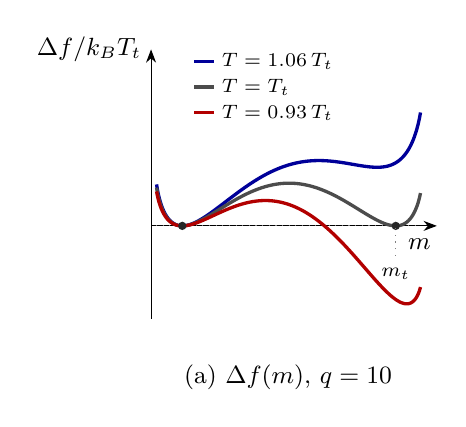
\begin{tikzpicture}[>=Stealth,font=\small,x=3.05cm,y=7.6cm]
  \draw[->] (-0.13,0) -- (1.06,0);
  \node[anchor=north east,inner sep=2pt] at (1.06,-0.012) {$m$};
  \draw[->] (-0.13,-0.155) -- (-0.13,0.295) node[left]{$\Delta f/k_BT_t$};
  \draw[dotted,gray] (-0.11,0) -- (0.99,0);
  \draw[very thick,blue!60!black] plot coordinates{(-0.10711,0.06926) (-0.10212,0.05746) (-0.09712,0.04837) (-0.09212,0.04093) (-0.08713,0.03467) (-0.08213,0.02932) (-0.07714,0.02471) (-0.07214,0.02072) (-0.06714,0.01724) (-0.06215,0.01422) (-0.05715,0.01160) (-0.05216,0.00934) (-0.04716,0.00738) (-0.04216,0.00572) (-0.03717,0.00431) (-0.03217,0.00313) (-0.02718,0.00217) (-0.02218,0.00141) (-0.01718,0.00082) (-0.01219,0.00040) (-0.00719,0.00014) (-0.00220,0.00001) (0.00280,0.00002) (0.00780,0.00015) (0.01279,0.00039) (0.01779,0.00074) (0.02278,0.00118) (0.02778,0.00172) (0.03278,0.00234) (0.03777,0.00304) (0.04277,0.00382) (0.04776,0.00466) (0.05276,0.00557) (0.05776,0.00654) (0.06275,0.00756) (0.06775,0.00863) (0.07274,0.00975) (0.07774,0.01092) (0.08274,0.01212) (0.08773,0.01336) (0.09273,0.01464) (0.09772,0.01595) (0.10272,0.01729) (0.10772,0.01866) (0.11271,0.02005) (0.11771,0.02146) (0.12270,0.02290) (0.12770,0.02435) (0.13269,0.02581) (0.13769,0.02729) (0.14269,0.02879) (0.14768,0.03029) (0.15268,0.03180) (0.15767,0.03332) (0.16267,0.03485) (0.16767,0.03638) (0.17266,0.03791) (0.17766,0.03945) (0.18265,0.04098) (0.18765,0.04252) (0.19265,0.04405) (0.19764,0.04558) (0.20264,0.04710) (0.20763,0.04862) (0.21263,0.05014) (0.21763,0.05164) (0.22262,0.05314) (0.22762,0.05463) (0.23261,0.05611) (0.23761,0.05758) (0.24261,0.05903) (0.24760,0.06048) (0.25260,0.06191) (0.25759,0.06333) (0.26259,0.06473) (0.26759,0.06612) (0.27258,0.06749) (0.27758,0.06885) (0.28257,0.07019) (0.28757,0.07151) (0.29257,0.07281) (0.29756,0.07410) (0.30256,0.07536) (0.30755,0.07661) (0.31255,0.07784) (0.31755,0.07905) (0.32254,0.08023) (0.32754,0.08140) (0.33253,0.08254) (0.33753,0.08367) (0.34253,0.08477) (0.34752,0.08585) (0.35252,0.08690) (0.35751,0.08793) (0.36251,0.08894) (0.36751,0.08993) (0.37250,0.09089) (0.37750,0.09183) (0.38249,0.09275) (0.38749,0.09364) (0.39248,0.09450) (0.39748,0.09534) (0.40248,0.09616) (0.40747,0.09695) (0.41247,0.09772) (0.41746,0.09846) (0.42246,0.09918) (0.42746,0.09987) (0.43245,0.10053) (0.43745,0.10118) (0.44244,0.10179) (0.44744,0.10238) (0.45244,0.10295) (0.45743,0.10349) (0.46243,0.10400) (0.46742,0.10449) (0.47242,0.10495) (0.47742,0.10539) (0.48241,0.10581) (0.48741,0.10619) (0.49240,0.10656) (0.49740,0.10690) (0.50240,0.10721) (0.50739,0.10750) (0.51239,0.10777) (0.51738,0.10801) (0.52238,0.10823) (0.52738,0.10842) (0.53237,0.10860) (0.53737,0.10874) (0.54236,0.10887) (0.54736,0.10897) (0.55236,0.10905) (0.55735,0.10911) (0.56235,0.10915) (0.56734,0.10916) (0.57234,0.10916) (0.57734,0.10913) (0.58233,0.10909) (0.58733,0.10902) (0.59232,0.10893) (0.59732,0.10883) (0.60232,0.10871) (0.60731,0.10857) (0.61231,0.10841) (0.61730,0.10824) (0.62230,0.10805) (0.62729,0.10784) (0.63229,0.10762) (0.63729,0.10739) (0.64228,0.10714) (0.64728,0.10688) (0.65227,0.10660) (0.65727,0.10632) (0.66227,0.10602) (0.66726,0.10572) (0.67226,0.10540) (0.67725,0.10508) (0.68225,0.10475) (0.68725,0.10442) (0.69224,0.10408) (0.69724,0.10373) (0.70223,0.10339) (0.70723,0.10304) (0.71223,0.10269) (0.71722,0.10234) (0.72222,0.10199) (0.72721,0.10165) (0.73221,0.10131) (0.73721,0.10098) (0.74220,0.10065) (0.74720,0.10033) (0.75219,0.10003) (0.75719,0.09973) (0.76219,0.09946) (0.76718,0.09919) (0.77218,0.09895) (0.77717,0.09873) (0.78217,0.09853) (0.78717,0.09835) (0.79216,0.09820) (0.79716,0.09808) (0.80215,0.09800) (0.80715,0.09795) (0.81215,0.09794) (0.81714,0.09796) (0.82214,0.09804) (0.82713,0.09816) (0.83213,0.09834) (0.83713,0.09857) (0.84212,0.09886) (0.84712,0.09921) (0.85211,0.09964) (0.85711,0.10014) (0.86211,0.10072) (0.86710,0.10138) (0.87210,0.10214) (0.87709,0.10300) (0.88209,0.10397) (0.88708,0.10505) (0.89208,0.10625) (0.89708,0.10759) (0.90207,0.10907) (0.90707,0.11071) (0.91206,0.11251) (0.91706,0.11450) (0.92206,0.11669) (0.92705,0.11909) (0.93205,0.12174) (0.93704,0.12464) (0.94204,0.12784) (0.94704,0.13136) (0.95203,0.13524) (0.95703,0.13953) (0.96202,0.14429) (0.96702,0.14959) (0.97202,0.15552) (0.97701,0.16222) (0.98201,0.16987) (0.98700,0.17878) (0.99200,0.18948)};
  \draw[very thick,gray!60!black] plot coordinates{(-0.10711,0.06390) (-0.10212,0.05289) (-0.09712,0.04444) (-0.09212,0.03755) (-0.08713,0.03175) (-0.08213,0.02681) (-0.07714,0.02256) (-0.07214,0.01889) (-0.06714,0.01570) (-0.06215,0.01293) (-0.05715,0.01054) (-0.05216,0.00847) (-0.04716,0.00669) (-0.04216,0.00517) (-0.03717,0.00389) (-0.03217,0.00283) (-0.02718,0.00196) (-0.02218,0.00127) (-0.01718,0.00074) (-0.01219,0.00036) (-0.00719,0.00012) (-0.00220,0.00001) (0.00280,0.00002) (0.00780,0.00013) (0.01279,0.00035) (0.01779,0.00066) (0.02278,0.00105) (0.02778,0.00153) (0.03278,0.00208) (0.03777,0.00269) (0.04277,0.00337) (0.04776,0.00411) (0.05276,0.00490) (0.05776,0.00575) (0.06275,0.00663) (0.06775,0.00756) (0.07274,0.00853) (0.07774,0.00954) (0.08274,0.01057) (0.08773,0.01164) (0.09273,0.01273) (0.09772,0.01385) (0.10272,0.01499) (0.10772,0.01614) (0.11271,0.01732) (0.11771,0.01850) (0.12270,0.01970) (0.12770,0.02092) (0.13269,0.02214) (0.13769,0.02336) (0.14269,0.02459) (0.14768,0.02583) (0.15268,0.02707) (0.15767,0.02831) (0.16267,0.02955) (0.16767,0.03078) (0.17266,0.03201) (0.17766,0.03324) (0.18265,0.03446) (0.18765,0.03568) (0.19265,0.03688) (0.19764,0.03808) (0.20264,0.03927) (0.20763,0.04044) (0.21263,0.04161) (0.21763,0.04276) (0.22262,0.04389) (0.22762,0.04501) (0.23261,0.04612) (0.23761,0.04721) (0.24261,0.04828) (0.24760,0.04933) (0.25260,0.05037) (0.25759,0.05139) (0.26259,0.05238) (0.26759,0.05336) (0.27258,0.05431) (0.27758,0.05525) (0.28257,0.05616) (0.28757,0.05705) (0.29257,0.05791) (0.29756,0.05875) (0.30256,0.05957) (0.30755,0.06036) (0.31255,0.06113) (0.31755,0.06187) (0.32254,0.06259) (0.32754,0.06328) (0.33253,0.06395) (0.33753,0.06458) (0.34253,0.06520) (0.34752,0.06578) (0.35252,0.06633) (0.35751,0.06686) (0.36251,0.06736) (0.36751,0.06783) (0.37250,0.06827) (0.37750,0.06869) (0.38249,0.06907) (0.38749,0.06943) (0.39248,0.06975) (0.39748,0.07005) (0.40248,0.07032) (0.40747,0.07056) (0.41247,0.07076) (0.41746,0.07094) (0.42246,0.07109) (0.42746,0.07121) (0.43245,0.07129) (0.43745,0.07135) (0.44244,0.07138) (0.44744,0.07138) (0.45244,0.07134) (0.45743,0.07128) (0.46243,0.07119) (0.46742,0.07106) (0.47242,0.07091) (0.47742,0.07072) (0.48241,0.07051) (0.48741,0.07027) (0.49240,0.06999) (0.49740,0.06969) (0.50240,0.06936) (0.50739,0.06900) (0.51239,0.06861) (0.51738,0.06819) (0.52238,0.06774) (0.52738,0.06726) (0.53237,0.06676) (0.53737,0.06623) (0.54236,0.06566) (0.54736,0.06508) (0.55236,0.06446) (0.55735,0.06382) (0.56235,0.06315) (0.56734,0.06245) (0.57234,0.06173) (0.57734,0.06098) (0.58233,0.06021) (0.58733,0.05941) (0.59232,0.05859) (0.59732,0.05774) (0.60232,0.05687) (0.60731,0.05598) (0.61231,0.05506) (0.61730,0.05413) (0.62230,0.05317) (0.62729,0.05219) (0.63229,0.05119) (0.63729,0.05017) (0.64228,0.04913) (0.64728,0.04807) (0.65227,0.04699) (0.65727,0.04590) (0.66227,0.04479) (0.66726,0.04367) (0.67226,0.04253) (0.67725,0.04138) (0.68225,0.04021) (0.68725,0.03903) (0.69224,0.03784) (0.69724,0.03664) (0.70223,0.03544) (0.70723,0.03422) (0.71223,0.03300) (0.71722,0.03177) (0.72222,0.03054) (0.72721,0.02930) (0.73221,0.02806) (0.73721,0.02682) (0.74220,0.02558) (0.74720,0.02435) (0.75219,0.02312) (0.75719,0.02189) (0.76219,0.02067) (0.76718,0.01946) (0.77218,0.01827) (0.77717,0.01708) (0.78217,0.01591) (0.78717,0.01476) (0.79216,0.01362) (0.79716,0.01251) (0.80215,0.01142) (0.80715,0.01036) (0.81215,0.00933) (0.81714,0.00834) (0.82214,0.00738) (0.82713,0.00645) (0.83213,0.00557) (0.83713,0.00474) (0.84212,0.00396) (0.84712,0.00323) (0.85211,0.00256) (0.85711,0.00196) (0.86211,0.00143) (0.86710,0.00097) (0.87210,0.00059) (0.87709,0.00030) (0.88209,0.00010) (0.88708,0.00001) (0.89208,0.00002) (0.89708,0.00016) (0.90207,0.00042) (0.90707,0.00083) (0.91206,0.00139) (0.91706,0.00211) (0.92206,0.00302) (0.92705,0.00413) (0.93205,0.00545) (0.93704,0.00702) (0.94204,0.00885) (0.94704,0.01099) (0.95203,0.01345) (0.95703,0.01630) (0.96202,0.01958) (0.96702,0.02336) (0.97202,0.02774) (0.97701,0.03283) (0.98201,0.03882) (0.98700,0.04599) (0.99200,0.05483)};
  \draw[very thick,red!70!black] plot coordinates{(-0.10711,0.05764) (-0.10212,0.04757) (-0.09712,0.03986) (-0.09212,0.03360) (-0.08713,0.02835) (-0.08213,0.02389) (-0.07714,0.02006) (-0.07214,0.01676) (-0.06714,0.01390) (-0.06215,0.01143) (-0.05715,0.00929) (-0.05216,0.00745) (-0.04716,0.00587) (-0.04216,0.00453) (-0.03717,0.00340) (-0.03217,0.00247) (-0.02718,0.00170) (-0.02218,0.00110) (-0.01718,0.00064) (-0.01219,0.00031) (-0.00719,0.00011) (-0.00220,0.00001) (0.00280,0.00002) (0.00780,0.00011) (0.01279,0.00030) (0.01779,0.00056) (0.02278,0.00090) (0.02778,0.00130) (0.03278,0.00176) (0.03777,0.00228) (0.04277,0.00285) (0.04776,0.00347) (0.05276,0.00413) (0.05776,0.00482) (0.06275,0.00556) (0.06775,0.00632) (0.07274,0.00711) (0.07774,0.00793) (0.08274,0.00877) (0.08773,0.00963) (0.09273,0.01050) (0.09772,0.01139) (0.10272,0.01229) (0.10772,0.01320) (0.11271,0.01412) (0.11771,0.01505) (0.12270,0.01598) (0.12770,0.01691) (0.13269,0.01784) (0.13769,0.01877) (0.14269,0.01970) (0.14768,0.02063) (0.15268,0.02154) (0.15767,0.02245) (0.16267,0.02336) (0.16767,0.02425) (0.17266,0.02513) (0.17766,0.02600) (0.18265,0.02686) (0.18765,0.02770) (0.19265,0.02852) (0.19764,0.02933) (0.20264,0.03012) (0.20763,0.03090) (0.21263,0.03165) (0.21763,0.03239) (0.22262,0.03310) (0.22762,0.03379) (0.23261,0.03446) (0.23761,0.03511) (0.24261,0.03574) (0.24760,0.03633) (0.25260,0.03691) (0.25759,0.03746) (0.26259,0.03798) (0.26759,0.03847) (0.27258,0.03894) (0.27758,0.03938) (0.28257,0.03979) (0.28757,0.04018) (0.29257,0.04053) (0.29756,0.04085) (0.30256,0.04115) (0.30755,0.04141) (0.31255,0.04164) (0.31755,0.04184) (0.32254,0.04201) (0.32754,0.04215) (0.33253,0.04225) (0.33753,0.04232) (0.34253,0.04236) (0.34752,0.04237) (0.35252,0.04234) (0.35751,0.04228) (0.36251,0.04218) (0.36751,0.04205) (0.37250,0.04189) (0.37750,0.04169) (0.38249,0.04145) (0.38749,0.04119) (0.39248,0.04088) (0.39748,0.04054) (0.40248,0.04017) (0.40747,0.03976) (0.41247,0.03932) (0.41746,0.03884) (0.42246,0.03832) (0.42746,0.03777) (0.43245,0.03718) (0.43745,0.03656) (0.44244,0.03590) (0.44744,0.03520) (0.45244,0.03447) (0.45743,0.03370) (0.46243,0.03290) (0.46742,0.03206) (0.47242,0.03119) (0.47742,0.03028) (0.48241,0.02933) (0.48741,0.02835) (0.49240,0.02734) (0.49740,0.02629) (0.50240,0.02520) (0.50739,0.02408) (0.51239,0.02292) (0.51738,0.02173) (0.52238,0.02050) (0.52738,0.01924) (0.53237,0.01795) (0.53737,0.01662) (0.54236,0.01526) (0.54736,0.01386) (0.55236,0.01244) (0.55735,0.01097) (0.56235,0.00948) (0.56734,0.00795) (0.57234,0.00640) (0.57734,0.00481) (0.58233,0.00318) (0.58733,0.00153) (0.59232,-0.00015) (0.59732,-0.00186) (0.60232,-0.00361) (0.60731,-0.00538) (0.61231,-0.00718) (0.61730,-0.00901) (0.62230,-0.01086) (0.62729,-0.01275) (0.63229,-0.01466) (0.63729,-0.01659) (0.64228,-0.01855) (0.64728,-0.02054) (0.65227,-0.02255) (0.65727,-0.02459) (0.66227,-0.02665) (0.66726,-0.02873) (0.67226,-0.03083) (0.67725,-0.03295) (0.68225,-0.03509) (0.68725,-0.03725) (0.69224,-0.03943) (0.69724,-0.04163) (0.70223,-0.04384) (0.70723,-0.04607) (0.71223,-0.04831) (0.71722,-0.05056) (0.72222,-0.05283) (0.72721,-0.05511) (0.73221,-0.05739) (0.73721,-0.05969) (0.74220,-0.06199) (0.74720,-0.06430) (0.75219,-0.06661) (0.75719,-0.06893) (0.76219,-0.07124) (0.76718,-0.07356) (0.77218,-0.07587) (0.77717,-0.07818) (0.78217,-0.08048) (0.78717,-0.08277) (0.79216,-0.08505) (0.79716,-0.08732) (0.80215,-0.08958) (0.80715,-0.09182) (0.81215,-0.09403) (0.81714,-0.09623) (0.82214,-0.09840) (0.82713,-0.10054) (0.83213,-0.10265) (0.83713,-0.10472) (0.84212,-0.10676) (0.84712,-0.10875) (0.85211,-0.11069) (0.85711,-0.11258) (0.86211,-0.11441) (0.86710,-0.11619) (0.87210,-0.11789) (0.87709,-0.11952) (0.88209,-0.12107) (0.88708,-0.12254) (0.89208,-0.12391) (0.89708,-0.12517) (0.90207,-0.12633) (0.90707,-0.12736) (0.91206,-0.12825) (0.91706,-0.12900) (0.92206,-0.12959) (0.92705,-0.13000) (0.93205,-0.13021) (0.93704,-0.13021) (0.94204,-0.12997) (0.94704,-0.12945) (0.95203,-0.12864) (0.95703,-0.12747) (0.96202,-0.12592) (0.96702,-0.12390) (0.97202,-0.12134) (0.97701,-0.11812) (0.98201,-0.11407) (0.98700,-0.10894) (0.99200,-0.10225)};
  \fill[gray!30!black] (0,0) circle (1.5pt);
  \fill[gray!30!black] (0.8889,0) circle (1.5pt);
  \node[anchor=north,font=\scriptsize] at (0.8889,-0.055) {$m_t$};
  \draw[dotted,gray] (0.8889,-0.050) -- (0.8889,0);
  \draw[very thick,blue!60!black] (0.05,0.275) -- (0.13,0.275);
  \node[anchor=west,font=\scriptsize,inner sep=1.5pt] at (0.145,0.275) {$T=1.06\,T_t$};
  \draw[very thick,gray!60!black] (0.05,0.232) -- (0.13,0.232);
  \node[anchor=west,font=\scriptsize,inner sep=1.5pt] at (0.145,0.232) {$T=T_t$};
  \draw[very thick,red!70!black] (0.05,0.189) -- (0.13,0.189);
  \node[anchor=west,font=\scriptsize,inner sep=1.5pt] at (0.145,0.189) {$T=0.93\,T_t$};
  \node[anchor=north,font=\small] at (0.44,-0.215) {(a) $\Delta f(m)$, $q=10$};
\end{tikzpicture}
\hfill
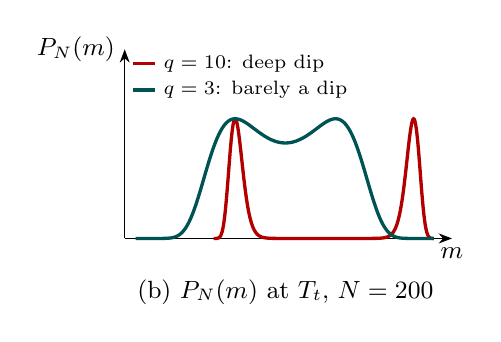
\begin{tikzpicture}[>=Stealth,font=\small,x=2.55cm,y=1.52cm]
  \draw[->] (-0.55,0) -- (1.08,0) node[below]{$m$};
  \draw[->] (-0.55,0) -- (-0.55,1.58) node[left]{$P_N(m)$};
  \draw[very thick,red!70!black] plot coordinates{(-0.10711,0.00000) (-0.10437,0.00001) (-0.10163,0.00003) (-0.09888,0.00008) (-0.09614,0.00018) (-0.09340,0.00039) (-0.09065,0.00079) (-0.08791,0.00147) (-0.08517,0.00262) (-0.08243,0.00444) (-0.07968,0.00722) (-0.07694,0.01131) (-0.07420,0.01711) (-0.07145,0.02510) (-0.06871,0.03578) (-0.06597,0.04966) (-0.06323,0.06725) (-0.06048,0.08901) (-0.05774,0.11532) (-0.05500,0.14646) (-0.05226,0.18255) (-0.04951,0.22357) (-0.04677,0.26931) (-0.04403,0.31936) (-0.04128,0.37315) (-0.03854,0.42994) (-0.03580,0.48884) (-0.03306,0.54885) (-0.03031,0.60890) (-0.02757,0.66787) (-0.02483,0.72466) (-0.02208,0.77821) (-0.01934,0.82752) (-0.01660,0.87173) (-0.01386,0.91011) (-0.01111,0.94207) (-0.00837,0.96721) (-0.00563,0.98526) (-0.00289,0.99617) (-0.00014,1.00000) (0.00260,0.99698) (0.00534,0.98746) (0.00809,0.97189) (0.01083,0.95081) (0.01357,0.92483) (0.01631,0.89459) (0.01906,0.86075) (0.02180,0.82399) (0.02454,0.78496) (0.02729,0.74429) (0.03003,0.70257) (0.03277,0.66035) (0.03551,0.61811) (0.03826,0.57630) (0.04100,0.53529) (0.04374,0.49540) (0.04648,0.45690) (0.04923,0.41999) (0.05197,0.38484) (0.05471,0.35156) (0.05746,0.32023) (0.06020,0.29088) (0.06294,0.26352) (0.06568,0.23814) (0.06843,0.21468) (0.07117,0.19308) (0.07391,0.17328) (0.07666,0.15518) (0.07940,0.13870) (0.08214,0.12374) (0.08488,0.11019) (0.08763,0.09796) (0.09037,0.08695) (0.09311,0.07706) (0.09585,0.06819) (0.09860,0.06027) (0.10134,0.05320) (0.10408,0.04690) (0.10683,0.04130) (0.10957,0.03633) (0.11231,0.03193) (0.11505,0.02804) (0.11780,0.02460) (0.12054,0.02157) (0.12328,0.01890) (0.12602,0.01654) (0.12877,0.01448) (0.13151,0.01266) (0.13425,0.01107) (0.13700,0.00967) (0.13974,0.00845) (0.14248,0.00738) (0.14522,0.00644) (0.14797,0.00563) (0.15071,0.00491) (0.15345,0.00429) (0.15620,0.00374) (0.15894,0.00327) (0.16168,0.00285) (0.16442,0.00249) (0.16717,0.00217) (0.16991,0.00190) (0.17265,0.00166) (0.17540,0.00145) (0.17814,0.00127) (0.18088,0.00111) (0.18362,0.00097) (0.18637,0.00085) (0.18911,0.00074) (0.19185,0.00065) (0.19459,0.00057) (0.19734,0.00050) (0.20008,0.00044) (0.20282,0.00038) (0.20557,0.00034) (0.20831,0.00030) (0.21105,0.00026) (0.21379,0.00023) (0.21654,0.00020) (0.21928,0.00018) (0.22202,0.00016) (0.22476,0.00014) (0.22751,0.00012) (0.23025,0.00011) (0.23299,0.00010) (0.23574,0.00009) (0.23848,0.00008) (0.24122,0.00007) (0.24396,0.00006) (0.24671,0.00005) (0.24945,0.00005) (0.25219,0.00004) (0.25494,0.00004) (0.25768,0.00003) (0.26042,0.00003) (0.26316,0.00003) (0.26591,0.00002) (0.26865,0.00002) (0.27139,0.00002) (0.27414,0.00002) (0.27688,0.00002) (0.27962,0.00001) (0.28236,0.00001) (0.28511,0.00001) (0.28785,0.00001) (0.29059,0.00001) (0.29333,0.00001) (0.29608,0.00001) (0.29882,0.00001) (0.30156,0.00001) (0.30431,0.00001) (0.30705,0.00001) (0.30979,0.00001) (0.31253,0.00000) (0.31528,0.00000) (0.31802,0.00000) (0.32076,0.00000) (0.32351,0.00000) (0.32625,0.00000) (0.32899,0.00000) (0.33173,0.00000) (0.33448,0.00000) (0.33722,0.00000) (0.33996,0.00000) (0.34270,0.00000) (0.34545,0.00000) (0.34819,0.00000) (0.35093,0.00000) (0.35368,0.00000) (0.35642,0.00000) (0.35916,0.00000) (0.36190,0.00000) (0.36465,0.00000) (0.36739,0.00000) (0.37013,0.00000) (0.37288,0.00000) (0.37562,0.00000) (0.37836,0.00000) (0.38110,0.00000) (0.38385,0.00000) (0.38659,0.00000) (0.38933,0.00000) (0.39207,0.00000) (0.39482,0.00000) (0.39756,0.00000) (0.40030,0.00000) (0.40305,0.00000) (0.40579,0.00000) (0.40853,0.00000) (0.41127,0.00000) (0.41402,0.00000) (0.41676,0.00000) (0.41950,0.00000) (0.42225,0.00000) (0.42499,0.00000) (0.42773,0.00000) (0.43047,0.00000) (0.43322,0.00000) (0.43596,0.00000) (0.43870,0.00000) (0.44144,0.00000) (0.44419,0.00000) (0.44693,0.00000) (0.44967,0.00000) (0.45242,0.00000) (0.45516,0.00000) (0.45790,0.00000) (0.46064,0.00000) (0.46339,0.00000) (0.46613,0.00000) (0.46887,0.00000) (0.47162,0.00000) (0.47436,0.00000) (0.47710,0.00000) (0.47984,0.00000) (0.48259,0.00000) (0.48533,0.00000) (0.48807,0.00000) (0.49081,0.00000) (0.49356,0.00000) (0.49630,0.00000) (0.49904,0.00000) (0.50179,0.00000) (0.50453,0.00000) (0.50727,0.00000) (0.51001,0.00000) (0.51276,0.00000) (0.51550,0.00000) (0.51824,0.00000) (0.52099,0.00000) (0.52373,0.00000) (0.52647,0.00000) (0.52921,0.00000) (0.53196,0.00000) (0.53470,0.00000) (0.53744,0.00000) (0.54018,0.00000) (0.54293,0.00000) (0.54567,0.00000) (0.54841,0.00000) (0.55116,0.00000) (0.55390,0.00000) (0.55664,0.00000) (0.55938,0.00000) (0.56213,0.00000) (0.56487,0.00000) (0.56761,0.00000) (0.57035,0.00000) (0.57310,0.00000) (0.57584,0.00000) (0.57858,0.00001) (0.58133,0.00001) (0.58407,0.00001) (0.58681,0.00001) (0.58955,0.00001) (0.59230,0.00001) (0.59504,0.00001) (0.59778,0.00001) (0.60053,0.00001) (0.60327,0.00001) (0.60601,0.00001) (0.60875,0.00001) (0.61150,0.00002) (0.61424,0.00002) (0.61698,0.00002) (0.61973,0.00002) (0.62247,0.00002) (0.62521,0.00003) (0.62795,0.00003) (0.63070,0.00003) (0.63344,0.00004) (0.63618,0.00004) (0.63892,0.00005) (0.64167,0.00005) (0.64441,0.00006) (0.64715,0.00007) (0.64990,0.00007) (0.65264,0.00008) (0.65538,0.00009) (0.65812,0.00011) (0.66087,0.00012) (0.66361,0.00014) (0.66635,0.00015) (0.66909,0.00018) (0.67184,0.00020) (0.67458,0.00023) (0.67732,0.00026) (0.68007,0.00029) (0.68281,0.00033) (0.68555,0.00038) (0.68829,0.00043) (0.69104,0.00049) (0.69378,0.00056) (0.69652,0.00063) (0.69927,0.00072) (0.70201,0.00083) (0.70475,0.00094) (0.70749,0.00108) (0.71024,0.00123) (0.71298,0.00141) (0.71572,0.00162) (0.71847,0.00185) (0.72121,0.00212) (0.72395,0.00243) (0.72669,0.00278) (0.72944,0.00318) (0.73218,0.00365) (0.73492,0.00418) (0.73766,0.00479) (0.74041,0.00548) (0.74315,0.00628) (0.74589,0.00720) (0.74864,0.00824) (0.75138,0.00943) (0.75412,0.01079) (0.75686,0.01235) (0.75961,0.01412) (0.76235,0.01614) (0.76509,0.01843) (0.76784,0.02104) (0.77058,0.02400) (0.77332,0.02736) (0.77606,0.03117) (0.77881,0.03547) (0.78155,0.04032) (0.78429,0.04580) (0.78703,0.05196) (0.78978,0.05888) (0.79252,0.06664) (0.79526,0.07532) (0.79801,0.08501) (0.80075,0.09580) (0.80349,0.10780) (0.80623,0.12109) (0.80898,0.13578) (0.81172,0.15197) (0.81446,0.16976) (0.81720,0.18923) (0.81995,0.21048) (0.82269,0.23359) (0.82543,0.25861) (0.82818,0.28560) (0.83092,0.31457) (0.83366,0.34554) (0.83640,0.37845) (0.83915,0.41326) (0.84189,0.44985) (0.84463,0.48807) (0.84738,0.52771) (0.85012,0.56854) (0.85286,0.61023) (0.85560,0.65242) (0.85835,0.69468) (0.86109,0.73653) (0.86383,0.77744) (0.86657,0.81682) (0.86932,0.85406) (0.87206,0.88849) (0.87480,0.91946) (0.87755,0.94629) (0.88029,0.96833) (0.88303,0.98498) (0.88577,0.99568) (0.88852,0.99995) (0.89126,0.99742) (0.89400,0.98785) (0.89675,0.97114) (0.89949,0.94732) (0.90223,0.91661) (0.90497,0.87940) (0.90772,0.83623) (0.91046,0.78781) (0.91320,0.73499) (0.91595,0.67873) (0.91869,0.62008) (0.92143,0.56015) (0.92417,0.50004) (0.92692,0.44086) (0.92966,0.38360) (0.93240,0.32918) (0.93514,0.27838) (0.93789,0.23180) (0.94063,0.18988) (0.94337,0.15285) (0.94612,0.12079) (0.94886,0.09358) (0.95160,0.07100) (0.95434,0.05266) (0.95709,0.03812) (0.95983,0.02688) (0.96257,0.01843) (0.96531,0.01225) (0.96806,0.00788) (0.97080,0.00488) (0.97354,0.00290) (0.97629,0.00165) (0.97903,0.00089) (0.98177,0.00045) (0.98451,0.00021) (0.98726,0.00009) (0.99000,0.00004)};
  \draw[very thick,teal!65!black] plot coordinates{(-0.49600,0.00000) (-0.49228,0.00000) (-0.48857,0.00000) (-0.48485,0.00000) (-0.48114,0.00000) (-0.47742,0.00000) (-0.47371,0.00000) (-0.46999,0.00000) (-0.46628,0.00000) (-0.46257,0.00000) (-0.45885,0.00000) (-0.45514,0.00000) (-0.45142,0.00000) (-0.44771,0.00000) (-0.44399,0.00000) (-0.44027,0.00000) (-0.43656,0.00000) (-0.43284,0.00000) (-0.42913,0.00000) (-0.42541,0.00000) (-0.42170,0.00000) (-0.41798,0.00000) (-0.41427,0.00000) (-0.41056,0.00000) (-0.40684,0.00000) (-0.40313,0.00001) (-0.39941,0.00001) (-0.39570,0.00001) (-0.39198,0.00002) (-0.38826,0.00003) (-0.38455,0.00004) (-0.38083,0.00005) (-0.37712,0.00008) (-0.37340,0.00011) (-0.36969,0.00015) (-0.36597,0.00020) (-0.36226,0.00027) (-0.35855,0.00036) (-0.35483,0.00048) (-0.35111,0.00063) (-0.34740,0.00081) (-0.34369,0.00105) (-0.33997,0.00134) (-0.33625,0.00170) (-0.33254,0.00215) (-0.32882,0.00269) (-0.32511,0.00334) (-0.32139,0.00411) (-0.31768,0.00504) (-0.31397,0.00614) (-0.31025,0.00743) (-0.30654,0.00894) (-0.30282,0.01069) (-0.29911,0.01271) (-0.29539,0.01503) (-0.29168,0.01769) (-0.28796,0.02070) (-0.28424,0.02410) (-0.28053,0.02793) (-0.27682,0.03222) (-0.27310,0.03699) (-0.26938,0.04228) (-0.26567,0.04812) (-0.26196,0.05454) (-0.25824,0.06156) (-0.25453,0.06921) (-0.25081,0.07750) (-0.24710,0.08647) (-0.24338,0.09613) (-0.23966,0.10648) (-0.23595,0.11754) (-0.23223,0.12932) (-0.22852,0.14181) (-0.22481,0.15502) (-0.22109,0.16893) (-0.21737,0.18354) (-0.21366,0.19883) (-0.20994,0.21479) (-0.20623,0.23139) (-0.20252,0.24859) (-0.19880,0.26639) (-0.19509,0.28473) (-0.19137,0.30358) (-0.18766,0.32290) (-0.18394,0.34265) (-0.18022,0.36278) (-0.17651,0.38325) (-0.17279,0.40400) (-0.16908,0.42499) (-0.16537,0.44615) (-0.16165,0.46745) (-0.15793,0.48882) (-0.15422,0.51022) (-0.15050,0.53159) (-0.14679,0.55287) (-0.14308,0.57403) (-0.13936,0.59501) (-0.13565,0.61575) (-0.13193,0.63622) (-0.12821,0.65637) (-0.12450,0.67616) (-0.12078,0.69555) (-0.11707,0.71449) (-0.11336,0.73296) (-0.10964,0.75093) (-0.10592,0.76836) (-0.10221,0.78522) (-0.09849,0.80150) (-0.09478,0.81717) (-0.09107,0.83221) (-0.08735,0.84661) (-0.08364,0.86036) (-0.07992,0.87344) (-0.07620,0.88585) (-0.07249,0.89759) (-0.06878,0.90864) (-0.06506,0.91902) (-0.06134,0.92872) (-0.05763,0.93774) (-0.05391,0.94610) (-0.05020,0.95379) (-0.04648,0.96084) (-0.04277,0.96725) (-0.03906,0.97303) (-0.03534,0.97820) (-0.03163,0.98278) (-0.02791,0.98677) (-0.02419,0.99020) (-0.02048,0.99308) (-0.01677,0.99543) (-0.01305,0.99727) (-0.00933,0.99863) (-0.00562,0.99951) (-0.00190,0.99995) (0.00181,0.99995) (0.00553,0.99955) (0.00924,0.99876) (0.01295,0.99760) (0.01667,0.99610) (0.02038,0.99427) (0.02410,0.99213) (0.02782,0.98970) (0.03153,0.98701) (0.03524,0.98407) (0.03896,0.98090) (0.04268,0.97751) (0.04639,0.97393) (0.05011,0.97018) (0.05382,0.96627) (0.05754,0.96221) (0.06125,0.95802) (0.06496,0.95373) (0.06868,0.94933) (0.07239,0.94485) (0.07611,0.94030) (0.07982,0.93570) (0.08354,0.93105) (0.08725,0.92637) (0.09097,0.92167) (0.09469,0.91696) (0.09840,0.91225) (0.10212,0.90755) (0.10583,0.90287) (0.10955,0.89822) (0.11326,0.89362) (0.11698,0.88905) (0.12069,0.88455) (0.12440,0.88010) (0.12812,0.87573) (0.13183,0.87143) (0.13555,0.86721) (0.13926,0.86308) (0.14298,0.85904) (0.14669,0.85510) (0.15041,0.85127) (0.15413,0.84754) (0.15784,0.84392) (0.16156,0.84042) (0.16527,0.83704) (0.16898,0.83378) (0.17270,0.83065) (0.17641,0.82765) (0.18013,0.82478) (0.18384,0.82205) (0.18756,0.81945) (0.19128,0.81699) (0.19499,0.81468) (0.19871,0.81250) (0.20242,0.81048) (0.20613,0.80860) (0.20985,0.80686) (0.21357,0.80528) (0.21728,0.80385) (0.22100,0.80256) (0.22471,0.80143) (0.22842,0.80046) (0.23214,0.79963) (0.23586,0.79897) (0.23957,0.79845) (0.24328,0.79809) (0.24700,0.79789) (0.25071,0.79784) (0.25443,0.79795) (0.25815,0.79821) (0.26186,0.79863) (0.26558,0.79920) (0.26929,0.79993) (0.27300,0.80081) (0.27672,0.80185) (0.28043,0.80304) (0.28415,0.80438) (0.28787,0.80587) (0.29158,0.80751) (0.29529,0.80930) (0.29901,0.81124) (0.30273,0.81332) (0.30644,0.81555) (0.31015,0.81792) (0.31387,0.82043) (0.31758,0.82308) (0.32130,0.82587) (0.32502,0.82879) (0.32873,0.83184) (0.33244,0.83502) (0.33616,0.83833) (0.33988,0.84176) (0.34359,0.84530) (0.34730,0.84896) (0.35102,0.85273) (0.35473,0.85661) (0.35845,0.86058) (0.36217,0.86466) (0.36588,0.86882) (0.36960,0.87307) (0.37331,0.87740) (0.37702,0.88181) (0.38074,0.88628) (0.38445,0.89080) (0.38817,0.89538) (0.39189,0.90001) (0.39560,0.90467) (0.39931,0.90935) (0.40303,0.91406) (0.40675,0.91877) (0.41046,0.92348) (0.41417,0.92817) (0.41789,0.93284) (0.42160,0.93748) (0.42532,0.94206) (0.42904,0.94658) (0.43275,0.95103) (0.43646,0.95539) (0.44018,0.95965) (0.44389,0.96379) (0.44761,0.96779) (0.45132,0.97164) (0.45504,0.97533) (0.45876,0.97884) (0.46247,0.98214) (0.46619,0.98523) (0.46990,0.98808) (0.47362,0.99067) (0.47733,0.99299) (0.48104,0.99501) (0.48476,0.99672) (0.48848,0.99809) (0.49219,0.99911) (0.49591,0.99975) (0.49962,1.00000) (0.50333,0.99983) (0.50705,0.99923) (0.51077,0.99816) (0.51448,0.99662) (0.51819,0.99459) (0.52191,0.99203) (0.52563,0.98894) (0.52934,0.98530) (0.53306,0.98109) (0.53677,0.97629) (0.54048,0.97088) (0.54420,0.96486) (0.54791,0.95821) (0.55163,0.95091) (0.55534,0.94296) (0.55906,0.93435) (0.56278,0.92506) (0.56649,0.91510) (0.57020,0.90447) (0.57392,0.89315) (0.57764,0.88116) (0.58135,0.86849) (0.58506,0.85515) (0.58878,0.84115) (0.59249,0.82650) (0.59621,0.81121) (0.59993,0.79530) (0.60364,0.77880) (0.60735,0.76171) (0.61107,0.74408) (0.61479,0.72591) (0.61850,0.70725) (0.62221,0.68814) (0.62593,0.66859) (0.62965,0.64866) (0.63336,0.62838) (0.63708,0.60780) (0.64079,0.58696) (0.64451,0.56591) (0.64822,0.54469) (0.65193,0.52337) (0.65565,0.50198) (0.65936,0.48059) (0.66308,0.45924) (0.66680,0.43799) (0.67051,0.41688) (0.67422,0.39598) (0.67794,0.37534) (0.68166,0.35499) (0.68537,0.33500) (0.68908,0.31541) (0.69280,0.29627) (0.69651,0.27761) (0.70023,0.25947) (0.70395,0.24190) (0.70766,0.22492) (0.71137,0.20857) (0.71509,0.19287) (0.71880,0.17783) (0.72252,0.16349) (0.72623,0.14985) (0.72995,0.13692) (0.73367,0.12470) (0.73738,0.11320) (0.74110,0.10241) (0.74481,0.09233) (0.74853,0.08294) (0.75224,0.07423) (0.75595,0.06619) (0.75967,0.05878) (0.76338,0.05200) (0.76710,0.04581) (0.77082,0.04018) (0.77453,0.03509) (0.77824,0.03051) (0.78196,0.02641) (0.78567,0.02274) (0.78939,0.01949) (0.79310,0.01662) (0.79682,0.01410) (0.80053,0.01190) (0.80425,0.00998) (0.80797,0.00833) (0.81168,0.00691) (0.81540,0.00570) (0.81911,0.00467) (0.82282,0.00380) (0.82654,0.00307) (0.83025,0.00247) (0.83397,0.00197) (0.83769,0.00156) (0.84140,0.00122) (0.84512,0.00095) (0.84883,0.00074) (0.85255,0.00056) (0.85626,0.00043) (0.85997,0.00032) (0.86369,0.00024) (0.86740,0.00018) (0.87112,0.00013) (0.87483,0.00009) (0.87855,0.00007) (0.88227,0.00005) (0.88598,0.00003) (0.88970,0.00002) (0.89341,0.00002) (0.89712,0.00001) (0.90084,0.00001) (0.90455,0.00000) (0.90827,0.00000) (0.91198,0.00000) (0.91570,0.00000) (0.91941,0.00000) (0.92313,0.00000) (0.92685,0.00000) (0.93056,0.00000) (0.93427,0.00000) (0.93799,0.00000) (0.94171,0.00000) (0.94542,0.00000) (0.94913,0.00000) (0.95285,0.00000) (0.95656,0.00000) (0.96028,0.00000) (0.96400,0.00000) (0.96771,0.00000) (0.97142,0.00000) (0.97514,0.00000) (0.97886,0.00000) (0.98257,0.00000) (0.98629,0.00000) (0.99000,0.00000)};
  \draw[very thick,red!70!black] (-0.51,1.46) -- (-0.40,1.46);
  \node[anchor=west,font=\scriptsize,inner sep=1.5pt] at (-0.38,1.46) {$q=10$: deep dip};
  \draw[very thick,teal!65!black] (-0.51,1.24) -- (-0.40,1.24);
  \node[anchor=west,font=\scriptsize,inner sep=1.5pt] at (-0.38,1.24) {$q=3$: barely a dip};
  \node[anchor=north,font=\small] at (0.25,-0.26) {(b) $P_N(m)$ at $T_t$, $N=200$};
\end{tikzpicture}

\vspace{2.5ex}
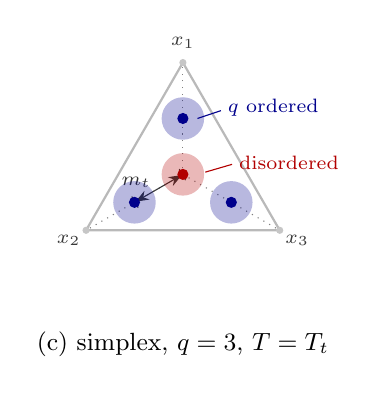
\begin{tikzpicture}[>=Stealth,font=\small,x=1.42cm,y=1.42cm]
  \draw[thick,gray!55] (90:1) -- (210:1) -- (330:1) -- cycle;
  \foreach \a/\lb in {90/$x_1$,210/$x_2$,330/$x_3$}{
     \fill[gray!45] (\a:1) circle (1.3pt);
     \node[font=\scriptsize,gray!45!black] at (\a:1.18) {\lb};}
  \foreach \a in {90,210,330}{\draw[dotted,gray] (0,0) -- (\a:1);}
  \draw[|<->|,thin,gray!45!black] (0,0) -- (210:0.5);
  \node[anchor=south east,font=\scriptsize,gray!40!black,inner sep=1pt] at (210:0.30) {$m_t$};
  \foreach \a in {90,210,330}{
     \fill[blue!55!black,opacity=0.28] (\a:0.5) circle (0.19);
     \fill[blue!55!black] (\a:0.5) circle (0.05);}
  \fill[red!70!black,opacity=0.28] (0,0) circle (0.19);
  \fill[red!70!black] (0,0) circle (0.05);
  \node[anchor=west,font=\scriptsize,blue!55!black,inner sep=1.5pt] at (0.36,0.60) {$q$ ordered};
  \draw[blue!55!black,thin] (0.34,0.57) -- (0.13,0.50);
  \node[anchor=west,font=\scriptsize,red!70!black,inner sep=1.5pt] at (0.46,0.10) {disordered};
  \draw[red!70!black,thin] (0.44,0.09) -- (0.20,0.02);
  \node[anchor=north,font=\small] at (0,-1.32) {(c) simplex, $q=3$, $T=T_t$};
\end{tikzpicture}
\hspace{0.02\textwidth}
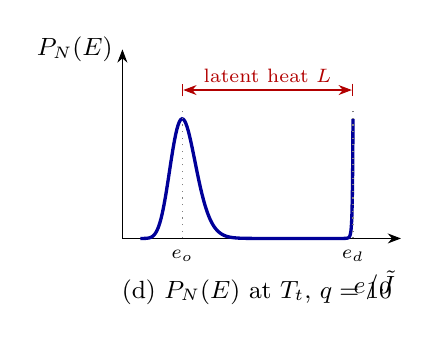
\begin{tikzpicture}[>=Stealth,font=\small,x=6.10cm,y=1.52cm]
  \draw[->] (-0.53,0) -- (0.05,0);
  \node[anchor=north east,inner sep=2pt] at (0.05,-0.22) {$e/\tilde J$};
  \draw[->] (-0.53,0) -- (-0.53,1.58) node[left]{$P_N(E)$};
  \draw[very thick,blue!60!black] plot coordinates{(-0.05000,1.00000) (-0.05000,0.99512) (-0.05002,0.98095) (-0.05004,0.95835) (-0.05008,0.92833) (-0.05012,0.89199) (-0.05018,0.85051) (-0.05024,0.80506) (-0.05031,0.75675) (-0.05040,0.70667) (-0.05049,0.65578) (-0.05060,0.60493) (-0.05071,0.55488) (-0.05083,0.50625) (-0.05096,0.45953) (-0.05111,0.41510) (-0.05126,0.37326) (-0.05142,0.33417) (-0.05159,0.29795) (-0.05178,0.26462) (-0.05197,0.23416) (-0.05217,0.20648) (-0.05238,0.18148) (-0.05260,0.15901) (-0.05283,0.13892) (-0.05308,0.12103) (-0.05333,0.10518) (-0.05359,0.09118) (-0.05386,0.07887) (-0.05414,0.06807) (-0.05443,0.05864) (-0.05473,0.05043) (-0.05504,0.04329) (-0.05536,0.03710) (-0.05569,0.03176) (-0.05603,0.02715) (-0.05638,0.02318) (-0.05674,0.01977) (-0.05710,0.01685) (-0.05748,0.01434) (-0.05787,0.01220) (-0.05827,0.01038) (-0.05868,0.00882) (-0.05910,0.00749) (-0.05953,0.00636) (-0.05996,0.00540) (-0.06041,0.00458) (-0.06087,0.00389) (-0.06134,0.00330) (-0.06181,0.00280) (-0.06230,0.00238) (-0.06280,0.00202) (-0.06330,0.00172) (-0.06382,0.00146) (-0.06435,0.00124) (-0.06488,0.00106) (-0.06543,0.00090) (-0.06599,0.00076) (-0.06655,0.00065) (-0.06713,0.00056) (-0.06771,0.00047) (-0.06831,0.00041) (-0.06891,0.00035) (-0.06953,0.00030) (-0.07015,0.00025) (-0.07079,0.00022) (-0.07143,0.00019) (-0.07209,0.00016) (-0.07275,0.00014) (-0.07343,0.00012) (-0.07411,0.00010) (-0.07480,0.00009) (-0.07551,0.00008) (-0.07622,0.00007) (-0.07694,0.00006) (-0.07768,0.00005) (-0.07842,0.00004) (-0.07917,0.00004) (-0.07994,0.00003) (-0.08071,0.00003) (-0.08149,0.00003) (-0.08228,0.00002) (-0.08308,0.00002) (-0.08390,0.00002) (-0.08472,0.00002) (-0.08555,0.00001) (-0.08639,0.00001) (-0.08724,0.00001) (-0.08810,0.00001) (-0.08897,0.00001) (-0.08985,0.00001) (-0.09075,0.00001) (-0.09165,0.00001) (-0.09256,0.00001) (-0.09348,0.00001) (-0.09441,0.00000) (-0.09535,0.00000) (-0.09630,0.00000) (-0.09725,0.00000) (-0.09822,0.00000) (-0.09920,0.00000) (-0.10019,0.00000) (-0.10119,0.00000) (-0.10220,0.00000) (-0.10322,0.00000) (-0.10425,0.00000) (-0.10528,0.00000) (-0.10633,0.00000) (-0.10739,0.00000) (-0.10846,0.00000) (-0.10954,0.00000) (-0.11062,0.00000) (-0.11172,0.00000) (-0.11283,0.00000) (-0.11394,0.00000) (-0.11507,0.00000) (-0.11621,0.00000) (-0.11735,0.00000) (-0.11851,0.00000) (-0.11968,0.00000) (-0.12085,0.00000) (-0.12204,0.00000) (-0.12323,0.00000) (-0.12444,0.00000) (-0.12565,0.00000) (-0.12688,0.00000) (-0.12812,0.00000) (-0.12936,0.00000) (-0.13061,0.00000) (-0.13188,0.00000) (-0.13315,0.00000) (-0.13444,0.00000) (-0.13573,0.00000) (-0.13704,0.00000) (-0.13835,0.00000) (-0.13967,0.00000) (-0.14101,0.00000) (-0.14235,0.00000) (-0.14370,0.00000) (-0.14507,0.00000) (-0.14644,0.00000) (-0.14782,0.00000) (-0.14921,0.00000) (-0.15062,0.00000) (-0.15203,0.00000) (-0.15345,0.00000) (-0.15488,0.00000) (-0.15632,0.00000) (-0.15777,0.00000) (-0.15924,0.00000) (-0.16071,0.00000) (-0.16219,0.00000) (-0.16368,0.00000) (-0.16518,0.00000) (-0.16669,0.00000) (-0.16821,0.00000) (-0.16974,0.00000) (-0.17128,0.00000) (-0.17283,0.00000) (-0.17439,0.00000) (-0.17596,0.00000) (-0.17754,0.00000) (-0.17913,0.00000) (-0.18073,0.00000) (-0.18234,0.00000) (-0.18396,0.00000) (-0.18558,0.00000) (-0.18722,0.00000) (-0.18887,0.00000) (-0.19053,0.00000) (-0.19220,0.00000) (-0.19388,0.00000) (-0.19556,0.00000) (-0.19726,0.00000) (-0.19897,0.00000) (-0.20068,0.00001) (-0.20241,0.00001) (-0.20415,0.00001) (-0.20590,0.00001) (-0.20765,0.00001) (-0.20942,0.00001) (-0.21119,0.00001) (-0.21298,0.00001) (-0.21478,0.00001) (-0.21658,0.00001) (-0.21840,0.00002) (-0.22022,0.00002) (-0.22206,0.00002) (-0.22390,0.00002) (-0.22576,0.00003) (-0.22762,0.00003) (-0.22950,0.00003) (-0.23138,0.00004) (-0.23328,0.00005) (-0.23518,0.00005) (-0.23710,0.00006) (-0.23902,0.00007) (-0.24095,0.00008) (-0.24290,0.00009) (-0.24485,0.00011) (-0.24681,0.00012) (-0.24879,0.00014) (-0.25077,0.00017) (-0.25276,0.00019) (-0.25476,0.00022) (-0.25678,0.00026) (-0.25880,0.00031) (-0.26083,0.00036) (-0.26287,0.00042) (-0.26492,0.00049) (-0.26699,0.00057) (-0.26906,0.00067) (-0.27114,0.00079) (-0.27323,0.00092) (-0.27533,0.00109) (-0.27744,0.00128) (-0.27956,0.00150) (-0.28169,0.00177) (-0.28383,0.00208) (-0.28598,0.00245) (-0.28814,0.00289) (-0.29031,0.00340) (-0.29249,0.00401) (-0.29468,0.00472) (-0.29688,0.00556) (-0.29909,0.00655) (-0.30131,0.00772) (-0.30354,0.00908) (-0.30578,0.01069) (-0.30803,0.01257) (-0.31028,0.01477) (-0.31255,0.01735) (-0.31483,0.02035) (-0.31712,0.02386) (-0.31942,0.02794) (-0.32172,0.03268) (-0.32404,0.03817) (-0.32637,0.04452) (-0.32871,0.05184) (-0.33105,0.06027) (-0.33341,0.06994) (-0.33578,0.08100) (-0.33815,0.09361) (-0.34054,0.10793) (-0.34294,0.12414) (-0.34534,0.14242) (-0.34776,0.16293) (-0.35018,0.18585) (-0.35262,0.21134) (-0.35506,0.23952) (-0.35752,0.27050) (-0.35999,0.30436) (-0.36246,0.34111) (-0.36494,0.38070) (-0.36744,0.42304) (-0.36994,0.46790) (-0.37246,0.51501) (-0.37498,0.56394) (-0.37752,0.61419) (-0.38006,0.66510) (-0.38261,0.71591) (-0.38518,0.76575) (-0.38775,0.81361) (-0.39033,0.85843) (-0.39293,0.89905) (-0.39553,0.93432) (-0.39814,0.96307) (-0.40076,0.98420) (-0.40340,0.99673) (-0.40604,0.99983) (-0.40869,0.99292) (-0.41135,0.97566) (-0.41402,0.94805) (-0.41671,0.91043) (-0.41940,0.86349) (-0.42210,0.80826) (-0.42481,0.74612) (-0.42753,0.67868) (-0.43026,0.60778) (-0.43300,0.53535) (-0.43575,0.46332) (-0.43851,0.39355) (-0.44128,0.32768) (-0.44406,0.26708) (-0.44685,0.21277) (-0.44965,0.16541) (-0.45246,0.12525) (-0.45528,0.09219) (-0.45811,0.06579) (-0.46095,0.04542) (-0.46380,0.03022) (-0.46666,0.01932) (-0.46953,0.01182) (-0.47240,0.00688) (-0.47529,0.00379) (-0.47819,0.00196) (-0.48110,0.00094) (-0.48402,0.00042) (-0.48694,0.00017) (-0.48988,0.00006) (-0.49283,0.00002)};
  \draw[dotted,gray] (-0.05,0) -- (-0.05,1.10);
  \draw[dotted,gray] (-0.40556,0) -- (-0.40556,1.10);
  \node[anchor=north,font=\scriptsize] at (-0.05,-0.02) {$e_d$};
  \node[anchor=north,font=\scriptsize] at (-0.40556,-0.02) {$e_o$};
  \draw[|<->|,thin,red!70!black] (-0.40556,1.24) -- (-0.05,1.24);
  \node[anchor=south,font=\scriptsize,red!70!black,inner sep=1.5pt] at (-0.228,1.26)
       {latent heat $L$};
  \node[anchor=north,font=\small] at (-0.25,-0.26) {(d) $P_N(E)$ at $T_t$, $q=10$};
\end{tikzpicture}
\caption{The mean-field $q$-state Potts model at its first-order transition.
\textbf{(a)} The exact constrained free energy for $q=10$. Above $T_t$ the
disordered minimum at $m=0$ is lowest; at $T_t$ it is exactly degenerate with the
ordered one at $m_t=(q-2)/(q-1)$; below $T_t$ the ordered one wins. Note the
manifest asymmetry in $m$ --- the cubic term of
Section~\ref{sec:apppotts:landau} --- which is what makes the transition first
order. \textbf{(b)} $P_N(m)\propto e^{-\beta Nf_N}$ at $T_t$, at the \emph{same}
$N$, for $q=10$ and $q=3$, each normalised to unit maximum. The barrier is $65$
times larger at $q=10$, so the same first-order transition is unmistakable at
$q=10$ and essentially invisible at $q=3$. \textbf{(c)} The full order-parameter
space is the simplex; at $T_t$ there are $q+1$ degenerate maxima --- the centroid
plus one at a fraction $m_t$ of the way to each of the $q$ vertices --- drawn here
for $q=3$, which is Figure~\ref{fig:histograms}d computed rather than sketched.
\textbf{(d)} $P_N(E)$ has only \emph{two} peaks, because the $q$ ordered states
are permutations of one another and therefore share an energy density; their
separation is the latent heat. Contrast Ising, where the two ordered states are
symmetry images and $P(E)$ has a single peak.}
\label{fig:apppotts1}
\end{figure}


\begin{figure}[htbp]
\centering
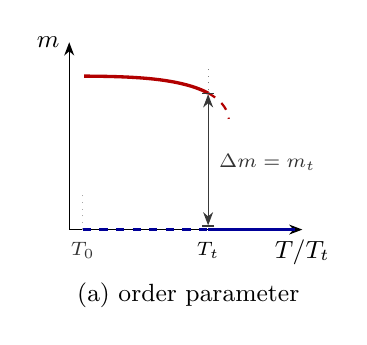
\begin{tikzpicture}[>=Stealth,font=\small,x=3.15cm,y=1.95cm]
  \draw[->] (0.44,0) -- (1.38,0) node[below]{$T/T_t$};
  \draw[->] (0.44,0) -- (0.44,1.22) node[left]{$m$};
  \draw[dotted,gray] (1,0) -- (1,1.08);
  \node[anchor=north,font=\scriptsize] at (1,-0.02) {$T_t$};
  \draw[very thick,red!70!black] plot coordinates{(0.50000,0.99949) (0.50455,0.99944) (0.50909,0.99939) (0.51364,0.99934) (0.51818,0.99928) (0.52273,0.99921) (0.52727,0.99915) (0.53182,0.99907) (0.53636,0.99900) (0.54091,0.99892) (0.54545,0.99883) (0.55000,0.99874) (0.55455,0.99864) (0.55909,0.99854) (0.56364,0.99843) (0.56818,0.99831) (0.57273,0.99819) (0.57727,0.99806) (0.58182,0.99793) (0.58636,0.99778) (0.59091,0.99763) (0.59545,0.99747) (0.60000,0.99731) (0.60455,0.99713) (0.60909,0.99695) (0.61364,0.99676) (0.61818,0.99655) (0.62273,0.99634) (0.62727,0.99612) (0.63182,0.99589) (0.63636,0.99564) (0.64091,0.99539) (0.64545,0.99513) (0.65000,0.99485) (0.65455,0.99456) (0.65909,0.99426) (0.66364,0.99395) (0.66818,0.99362) (0.67273,0.99328) (0.67727,0.99293) (0.68182,0.99256) (0.68636,0.99218) (0.69091,0.99178) (0.69545,0.99137) (0.70000,0.99094) (0.70455,0.99050) (0.70909,0.99004) (0.71364,0.98956) (0.71818,0.98906) (0.72273,0.98855) (0.72727,0.98802) (0.73182,0.98747) (0.73636,0.98690) (0.74091,0.98631) (0.74545,0.98570) (0.75000,0.98507) (0.75455,0.98441) (0.75909,0.98374) (0.76364,0.98304) (0.76818,0.98232) (0.77273,0.98158) (0.77727,0.98081) (0.78182,0.98001) (0.78636,0.97919) (0.79091,0.97834) (0.79545,0.97747) (0.80000,0.97657) (0.80455,0.97564) (0.80909,0.97468) (0.81364,0.97368) (0.81818,0.97266) (0.82273,0.97161) (0.82727,0.97052) (0.83182,0.96940) (0.83636,0.96825) (0.84091,0.96705) (0.84545,0.96583) (0.85000,0.96456) (0.85455,0.96325) (0.85909,0.96191) (0.86364,0.96052) (0.86818,0.95909) (0.87273,0.95761) (0.87727,0.95609) (0.88182,0.95452) (0.88636,0.95291) (0.89091,0.95124) (0.89545,0.94952) (0.90000,0.94774) (0.90455,0.94591) (0.90909,0.94402) (0.91364,0.94207) (0.91818,0.94006) (0.92273,0.93798) (0.92727,0.93584) (0.93182,0.93362) (0.93636,0.93132) (0.94091,0.92895) (0.94545,0.92650) (0.95000,0.92397) (0.95455,0.92134) (0.95909,0.91862) (0.96364,0.91580) (0.96818,0.91288) (0.97273,0.90984) (0.97727,0.90669) (0.98182,0.90341) (0.98636,0.90001) (0.99091,0.89646) (0.99545,0.89275) (1.00000,0.88889)};
  \draw[thick,red!70!black,dashed] plot coordinates{(1.00000,0.88889) (1.00139,0.88767) (1.00278,0.88644) (1.00417,0.88519) (1.00556,0.88392) (1.00695,0.88263) (1.00834,0.88133) (1.00973,0.88000) (1.01112,0.87866) (1.01251,0.87730) (1.01390,0.87591) (1.01529,0.87450) (1.01668,0.87308) (1.01807,0.87162) (1.01946,0.87015) (1.02085,0.86865) (1.02224,0.86713) (1.02363,0.86558) (1.02502,0.86400) (1.02641,0.86240) (1.02780,0.86077) (1.02919,0.85911) (1.03058,0.85741) (1.03197,0.85569) (1.03336,0.85393) (1.03475,0.85214) (1.03614,0.85031) (1.03753,0.84845) (1.03892,0.84655) (1.04031,0.84460) (1.04170,0.84262) (1.04309,0.84058) (1.04449,0.83851) (1.04588,0.83638) (1.04727,0.83420) (1.04866,0.83196) (1.05005,0.82967) (1.05144,0.82731) (1.05283,0.82489) (1.05422,0.82240) (1.05561,0.81984) (1.05700,0.81719) (1.05839,0.81446) (1.05978,0.81164) (1.06117,0.80871) (1.06256,0.80567) (1.06395,0.80251) (1.06534,0.79922) (1.06673,0.79578) (1.06812,0.79217) (1.06951,0.78837) (1.07090,0.78436) (1.07229,0.78010) (1.07368,0.77554) (1.07507,0.77062) (1.07646,0.76527) (1.07785,0.75935) (1.07924,0.75266) (1.08063,0.74486) (1.08202,0.73519) (1.08341,0.72122)};
  \draw[very thick,blue!60!black] (1.0,0) -- (1.35,0);
  \draw[thick,blue!60!black,dashed] (0.4944,0) -- (1.0,0);
  \draw[|<->|,thin,gray!45!black] (1.0,0.02) -- (1.0,0.8889);
  \node[anchor=west,font=\scriptsize,gray!40!black,inner sep=2pt] at (1.02,0.44) {$\Delta m=m_t$};
  \draw[dotted,gray!70] (0.4944,0) -- (0.4944,0.24);
  \node[anchor=north,font=\scriptsize,gray!40!black] at (0.4944,-0.02) {$T_0$};
  \node[anchor=north,font=\small] at (0.92,-0.28) {(a) order parameter};
\end{tikzpicture}
\hfill
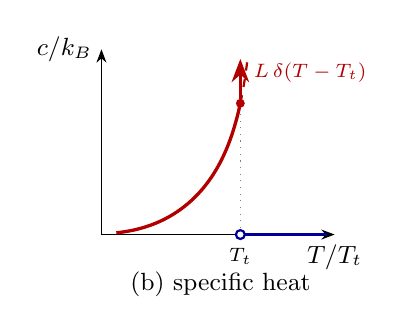
\begin{tikzpicture}[>=Stealth,font=\small,x=3.15cm,y=0.485cm]
  \draw[->] (0.44,0) -- (1.38,0) node[below]{$T/T_t$};
  \draw[->] (0.44,0) -- (0.44,4.85) node[left]{$c/k_B$};
  \draw[dotted,gray] (1,0) -- (1,4.55);
  \node[anchor=north,font=\scriptsize] at (1,-0.10) {$T_t$};
  \draw[very thick,red!70!black] plot coordinates{(0.50000,0.04507) (0.50455,0.04842) (0.50909,0.05194) (0.51364,0.05564) (0.51818,0.05954) (0.52273,0.06362) (0.52727,0.06790) (0.53182,0.07238) (0.53636,0.07706) (0.54091,0.08196) (0.54545,0.08707) (0.55000,0.09241) (0.55455,0.09796) (0.55909,0.10375) (0.56364,0.10977) (0.56818,0.11603) (0.57273,0.12254) (0.57727,0.12929) (0.58182,0.13629) (0.58636,0.14356) (0.59091,0.15108) (0.59545,0.15887) (0.60000,0.16694) (0.60455,0.17527) (0.60909,0.18389) (0.61364,0.19280) (0.61818,0.20199) (0.62273,0.21148) (0.62727,0.22127) (0.63182,0.23137) (0.63636,0.24177) (0.64091,0.25249) (0.64545,0.26352) (0.65000,0.27488) (0.65455,0.28657) (0.65909,0.29860) (0.66364,0.31096) (0.66818,0.32368) (0.67273,0.33674) (0.67727,0.35016) (0.68182,0.36395) (0.68636,0.37810) (0.69091,0.39263) (0.69545,0.40755) (0.70000,0.42285) (0.70455,0.43855) (0.70909,0.45466) (0.71364,0.47118) (0.71818,0.48811) (0.72273,0.50548) (0.72727,0.52328) (0.73182,0.54153) (0.73636,0.56023) (0.74091,0.57939) (0.74545,0.59903) (0.75000,0.61916) (0.75455,0.63977) (0.75909,0.66090) (0.76364,0.68255) (0.76818,0.70472) (0.77273,0.72745) (0.77727,0.75073) (0.78182,0.77458) (0.78636,0.79903) (0.79091,0.82408) (0.79545,0.84975) (0.80000,0.87607) (0.80455,0.90304) (0.80909,0.93069) (0.81364,0.95905) (0.81818,0.98813) (0.82273,1.01795) (0.82727,1.04855) (0.83182,1.07995) (0.83636,1.11218) (0.84091,1.14527) (0.84545,1.17925) (0.85000,1.21416) (0.85455,1.25003) (0.85909,1.28690) (0.86364,1.32482) (0.86818,1.36383) (0.87273,1.40399) (0.87727,1.44533) (0.88182,1.48792) (0.88636,1.53183) (0.89091,1.57711) (0.89545,1.62383) (0.90000,1.67209) (0.90455,1.72195) (0.90909,1.77351) (0.91364,1.82687) (0.91818,1.88214) (0.92273,1.93943) (0.92727,1.99889) (0.93182,2.06065) (0.93636,2.12488) (0.94091,2.19174) (0.94545,2.26145) (0.95000,2.33421) (0.95455,2.41028) (0.95909,2.48992) (0.96364,2.57345) (0.96818,2.66123) (0.97273,2.75366) (0.97727,2.85119) (0.98182,2.95436) (0.98636,3.06378) (0.99091,3.18016) (0.99545,3.30435) (1.00000,3.43735)};
  \draw[thick,red!70!black,dashed] plot coordinates{(1.00000,3.43735) (1.00028,3.44587) (1.00056,3.45443) (1.00084,3.46303) (1.00112,3.47167) (1.00140,3.48035) (1.00168,3.48907) (1.00196,3.49783) (1.00224,3.50663) (1.00253,3.51547) (1.00281,3.52435) (1.00309,3.53327) (1.00337,3.54223) (1.00365,3.55124) (1.00393,3.56028) (1.00421,3.56937) (1.00449,3.57851) (1.00477,3.58768) (1.00505,3.59690) (1.00533,3.60617) (1.00561,3.61548) (1.00589,3.62483) (1.00617,3.63423) (1.00645,3.64367) (1.00673,3.65316) (1.00701,3.66270) (1.00730,3.67228) (1.00758,3.68191) (1.00786,3.69159) (1.00814,3.70132) (1.00842,3.71110) (1.00870,3.72092) (1.00898,3.73079) (1.00926,3.74072) (1.00954,3.75069) (1.00982,3.76072) (1.01010,3.77079) (1.01038,3.78092) (1.01066,3.79110) (1.01094,3.80133) (1.01122,3.81162) (1.01150,3.82196) (1.01179,3.83235) (1.01207,3.84280) (1.01235,3.85331) (1.01263,3.86387) (1.01291,3.87448) (1.01319,3.88515) (1.01347,3.89588) (1.01375,3.90667) (1.01403,3.91752) (1.01431,3.92842) (1.01459,3.93939) (1.01487,3.95041) (1.01515,3.96150) (1.01543,3.97265) (1.01571,3.98386) (1.01599,3.99513) (1.01627,4.00646) (1.01656,4.01786) (1.01684,4.02933) (1.01712,4.04086) (1.01740,4.05245) (1.01768,4.06411) (1.01796,4.07584) (1.01824,4.08764) (1.01852,4.09950) (1.01880,4.11144) (1.01908,4.12344) (1.01936,4.13552) (1.01964,4.14766) (1.01992,4.15988) (1.02020,4.17217) (1.02048,4.18454) (1.02076,4.19698) (1.02104,4.20950) (1.02133,4.22209) (1.02161,4.23476) (1.02189,4.24751) (1.02217,4.26033) (1.02245,4.27324) (1.02273,4.28622) (1.02301,4.29929) (1.02329,4.31244) (1.02357,4.32568) (1.02385,4.33899) (1.02413,4.35240) (1.02441,4.36589) (1.02469,4.37946) (1.02497,4.39313) (1.02525,4.40688) (1.02553,4.42073) (1.02582,4.43466) (1.02610,4.44869) (1.02638,4.46281) (1.02666,4.47703) (1.02694,4.49134) (1.02722,4.50575) (1.02750,4.52025) (1.02778,4.53486) (1.02806,4.54956)};
  \draw[very thick,blue!60!black] (1.0,0) -- (1.35,0);
  \fill[red!70!black] (1.0,3.4373) circle (1.6pt);
  \draw[blue!60!black,fill=white,thick] (1.0,0) circle (1.6pt);
  \draw[->,very thick,red!70!black] (1.0,3.5573) -- (1.0,4.60);
  \node[anchor=west,font=\scriptsize,red!70!black,inner sep=2pt] at (1.03,4.25)
       {$L\,\delta(T-T_t)$};
  \node[anchor=north,font=\small] at (0.92,-0.72) {(b) specific heat};
\end{tikzpicture}

\vspace{2ex}
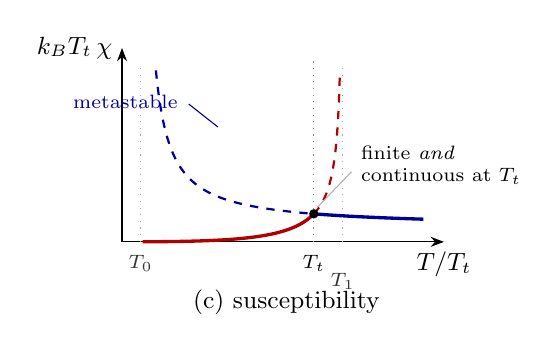
\begin{tikzpicture}[>=Stealth,font=\small,x=4.35cm,y=1.62cm]
  \draw[->] (0.44,0) -- (1.38,0) node[below]{$T/T_t$};
  \draw[->] (0.44,0) -- (0.44,1.52) node[left]{$k_BT_t\,\chi$};
  \draw[dotted,gray] (1,0) -- (1,1.42);
  \node[anchor=north,font=\scriptsize] at (1,-0.03) {$T_t$};
  \draw[dotted,gray!70] (0.4944,0) -- (0.4944,1.40);
  \node[anchor=north,font=\scriptsize,gray!40!black] at (0.4944,-0.03) {$T_0$};
  \draw[dotted,gray!70] (1.0842,0) -- (1.0842,1.40);
  \node[anchor=north,font=\scriptsize,gray!40!black] at (1.0842,-0.17) {$T_1$};
  \draw[very thick,red!70!black] plot coordinates{(0.50000,0.00057) (0.50455,0.00062) (0.50909,0.00068) (0.51364,0.00074) (0.51818,0.00081) (0.52273,0.00088) (0.52727,0.00096) (0.53182,0.00104) (0.53636,0.00112) (0.54091,0.00121) (0.54545,0.00131) (0.55000,0.00142) (0.55455,0.00153) (0.55909,0.00164) (0.56364,0.00177) (0.56818,0.00190) (0.57273,0.00204) (0.57727,0.00218) (0.58182,0.00234) (0.58636,0.00250) (0.59091,0.00268) (0.59545,0.00286) (0.60000,0.00305) (0.60455,0.00325) (0.60909,0.00347) (0.61364,0.00369) (0.61818,0.00393) (0.62273,0.00417) (0.62727,0.00443) (0.63182,0.00470) (0.63636,0.00499) (0.64091,0.00529) (0.64545,0.00560) (0.65000,0.00593) (0.65455,0.00627) (0.65909,0.00663) (0.66364,0.00700) (0.66818,0.00739) (0.67273,0.00780) (0.67727,0.00823) (0.68182,0.00867) (0.68636,0.00914) (0.69091,0.00962) (0.69545,0.01013) (0.70000,0.01066) (0.70455,0.01121) (0.70909,0.01178) (0.71364,0.01238) (0.71818,0.01300) (0.72273,0.01365) (0.72727,0.01432) (0.73182,0.01502) (0.73636,0.01575) (0.74091,0.01651) (0.74545,0.01731) (0.75000,0.01813) (0.75455,0.01899) (0.75909,0.01988) (0.76364,0.02080) (0.76818,0.02177) (0.77273,0.02277) (0.77727,0.02382) (0.78182,0.02490) (0.78636,0.02603) (0.79091,0.02720) (0.79545,0.02843) (0.80000,0.02970) (0.80455,0.03102) (0.80909,0.03240) (0.81364,0.03383) (0.81818,0.03532) (0.82273,0.03687) (0.82727,0.03848) (0.83182,0.04017) (0.83636,0.04192) (0.84091,0.04374) (0.84545,0.04564) (0.85000,0.04763) (0.85455,0.04969) (0.85909,0.05185) (0.86364,0.05410) (0.86818,0.05645) (0.87273,0.05890) (0.87727,0.06147) (0.88182,0.06415) (0.88636,0.06695) (0.89091,0.06988) (0.89545,0.07295) (0.90000,0.07617) (0.90455,0.07954) (0.90909,0.08308) (0.91364,0.08679) (0.91818,0.09070) (0.92273,0.09481) (0.92727,0.09913) (0.93182,0.10369) (0.93636,0.10850) (0.94091,0.11358) (0.94545,0.11895) (0.95000,0.12465) (0.95455,0.13068) (0.95909,0.13710) (0.96364,0.14393) (0.96818,0.15121) (0.97273,0.15899) (0.97727,0.16732) (0.98182,0.17626) (0.98636,0.18588) (0.99091,0.19627) (0.99545,0.20752) (1.00000,0.21975)};
  \draw[thick,red!70!black,dashed] plot coordinates{(1.00000,0.21975) (1.00021,0.22034) (1.00042,0.22094) (1.00063,0.22153) (1.00084,0.22213) (1.00105,0.22273) (1.00126,0.22334) (1.00147,0.22394) (1.00168,0.22455) (1.00189,0.22516) (1.00210,0.22578) (1.00231,0.22639) (1.00252,0.22701) (1.00274,0.22763) (1.00295,0.22826) (1.00316,0.22889) (1.00337,0.22951) (1.00358,0.23015) (1.00379,0.23078) (1.00400,0.23142) (1.00421,0.23206) (1.00442,0.23270) (1.00463,0.23335) (1.00484,0.23400) (1.00505,0.23465) (1.00526,0.23530) (1.00547,0.23596) (1.00568,0.23662) (1.00589,0.23728) (1.00610,0.23794) (1.00631,0.23861) (1.00652,0.23928) (1.00673,0.23996) (1.00694,0.24063) (1.00715,0.24131) (1.00736,0.24199) (1.00757,0.24268) (1.00778,0.24337) (1.00800,0.24406) (1.00821,0.24476) (1.00842,0.24545) (1.00863,0.24615) (1.00884,0.24686) (1.00905,0.24757) (1.00926,0.24828) (1.00947,0.24899) (1.00968,0.24971) (1.00989,0.25043) (1.01010,0.25115) (1.01031,0.25188) (1.01052,0.25261) (1.01073,0.25334) (1.01094,0.25408) (1.01115,0.25482) (1.01136,0.25556) (1.01157,0.25630) (1.01178,0.25706) (1.01199,0.25781) (1.01220,0.25857) (1.01241,0.25933) (1.01262,0.26009) (1.01283,0.26086) (1.01304,0.26163) (1.01326,0.26240) (1.01347,0.26318) (1.01368,0.26397) (1.01389,0.26475) (1.01410,0.26554) (1.01431,0.26634) (1.01452,0.26713) (1.01473,0.26793) (1.01494,0.26874) (1.01515,0.26955) (1.01536,0.27036) (1.01557,0.27118) (1.01578,0.27200) (1.01599,0.27282) (1.01620,0.27365) (1.01641,0.27448) (1.01662,0.27532) (1.01683,0.27616) (1.01704,0.27701) (1.01725,0.27786) (1.01746,0.27871) (1.01767,0.27957) (1.01788,0.28043) (1.01809,0.28130) (1.01830,0.28217) (1.01852,0.28304) (1.01873,0.28392) (1.01894,0.28481) (1.01915,0.28570) (1.01936,0.28659) (1.01957,0.28749) (1.01978,0.28839) (1.01999,0.28930) (1.02020,0.29021) (1.02041,0.29113) (1.02062,0.29205) (1.02083,0.29297) (1.02104,0.29390) (1.02125,0.29484) (1.02146,0.29578) (1.02167,0.29673) (1.02188,0.29768) (1.02209,0.29863) (1.02230,0.29959) (1.02251,0.30056) (1.02272,0.30153) (1.02293,0.30251) (1.02314,0.30349) (1.02335,0.30448) (1.02356,0.30547) (1.02378,0.30647) (1.02399,0.30747) (1.02420,0.30848) (1.02441,0.30950) (1.02462,0.31052) (1.02483,0.31154) (1.02504,0.31257) (1.02525,0.31361) (1.02546,0.31465) (1.02567,0.31570) (1.02588,0.31676) (1.02609,0.31782) (1.02630,0.31888) (1.02651,0.31996) (1.02672,0.32104) (1.02693,0.32212) (1.02714,0.32321) (1.02735,0.32431) (1.02756,0.32542) (1.02777,0.32653) (1.02798,0.32764) (1.02819,0.32877) (1.02840,0.32990) (1.02861,0.33103) (1.02882,0.33218) (1.02904,0.33333) (1.02925,0.33449) (1.02946,0.33565) (1.02967,0.33682) (1.02988,0.33800) (1.03009,0.33918) (1.03030,0.34038) (1.03051,0.34158) (1.03072,0.34278) (1.03093,0.34400) (1.03114,0.34522) (1.03135,0.34645) (1.03156,0.34769) (1.03177,0.34893) (1.03198,0.35019) (1.03219,0.35145) (1.03240,0.35272) (1.03261,0.35399) (1.03282,0.35528) (1.03303,0.35657) (1.03324,0.35787) (1.03345,0.35918) (1.03366,0.36050) (1.03387,0.36183) (1.03408,0.36316) (1.03430,0.36451) (1.03451,0.36586) (1.03472,0.36722) (1.03493,0.36859) (1.03514,0.36997) (1.03535,0.37136) (1.03556,0.37276) (1.03577,0.37417) (1.03598,0.37559) (1.03619,0.37701) (1.03640,0.37845) (1.03661,0.37990) (1.03682,0.38135) (1.03703,0.38282) (1.03724,0.38430) (1.03745,0.38578) (1.03766,0.38728) (1.03787,0.38879) (1.03808,0.39031) (1.03829,0.39184) (1.03850,0.39338) (1.03871,0.39493) (1.03892,0.39649) (1.03913,0.39806) (1.03934,0.39965) (1.03955,0.40124) (1.03977,0.40285) (1.03998,0.40447) (1.04019,0.40610) (1.04040,0.40775) (1.04061,0.40940) (1.04082,0.41107) (1.04103,0.41275) (1.04124,0.41445) (1.04145,0.41615) (1.04166,0.41787) (1.04187,0.41961) (1.04208,0.42135) (1.04229,0.42311) (1.04250,0.42488) (1.04271,0.42667) (1.04292,0.42847) (1.04313,0.43029) (1.04334,0.43212) (1.04355,0.43396) (1.04376,0.43582) (1.04397,0.43769) (1.04418,0.43958) (1.04439,0.44149) (1.04460,0.44341) (1.04481,0.44534) (1.04503,0.44729) (1.04524,0.44926) (1.04545,0.45124) (1.04566,0.45325) (1.04587,0.45526) (1.04608,0.45730) (1.04629,0.45935) (1.04650,0.46142) (1.04671,0.46351) (1.04692,0.46561) (1.04713,0.46773) (1.04734,0.46988) (1.04755,0.47204) (1.04776,0.47422) (1.04797,0.47642) (1.04818,0.47864) (1.04839,0.48087) (1.04860,0.48313) (1.04881,0.48541) (1.04902,0.48771) (1.04923,0.49004) (1.04944,0.49238) (1.04965,0.49474) (1.04986,0.49713) (1.05007,0.49954) (1.05029,0.50197) (1.05050,0.50443) (1.05071,0.50691) (1.05092,0.50941) (1.05113,0.51194) (1.05134,0.51449) (1.05155,0.51707) (1.05176,0.51967) (1.05197,0.52230) (1.05218,0.52495) (1.05239,0.52763) (1.05260,0.53034) (1.05281,0.53308) (1.05302,0.53584) (1.05323,0.53864) (1.05344,0.54146) (1.05365,0.54431) (1.05386,0.54719) (1.05407,0.55011) (1.05428,0.55305) (1.05449,0.55603) (1.05470,0.55903) (1.05491,0.56208) (1.05512,0.56515) (1.05533,0.56826) (1.05555,0.57140) (1.05576,0.57458) (1.05597,0.57779) (1.05618,0.58104) (1.05639,0.58433) (1.05660,0.58766) (1.05681,0.59103) (1.05702,0.59443) (1.05723,0.59788) (1.05744,0.60136) (1.05765,0.60489) (1.05786,0.60846) (1.05807,0.61208) (1.05828,0.61573) (1.05849,0.61944) (1.05870,0.62319) (1.05891,0.62699) (1.05912,0.63083) (1.05933,0.63473) (1.05954,0.63868) (1.05975,0.64267) (1.05996,0.64672) (1.06017,0.65083) (1.06038,0.65499) (1.06059,0.65920) (1.06081,0.66347) (1.06102,0.66781) (1.06123,0.67220) (1.06144,0.67665) (1.06165,0.68116) (1.06186,0.68574) (1.06207,0.69039) (1.06228,0.69510) (1.06249,0.69988) (1.06270,0.70474) (1.06291,0.70966) (1.06312,0.71466) (1.06333,0.71974) (1.06354,0.72489) (1.06375,0.73013) (1.06396,0.73544) (1.06417,0.74084) (1.06438,0.74633) (1.06459,0.75190) (1.06480,0.75757) (1.06501,0.76333) (1.06522,0.76919) (1.06543,0.77514) (1.06564,0.78120) (1.06585,0.78736) (1.06607,0.79363) (1.06628,0.80002) (1.06649,0.80651) (1.06670,0.81312) (1.06691,0.81986) (1.06712,0.82672) (1.06733,0.83371) (1.06754,0.84083) (1.06775,0.84809) (1.06796,0.85549) (1.06817,0.86303) (1.06838,0.87073) (1.06859,0.87858) (1.06880,0.88659) (1.06901,0.89478) (1.06922,0.90313) (1.06943,0.91166) (1.06964,0.92038) (1.06985,0.92929) (1.07006,0.93840) (1.07027,0.94772) (1.07048,0.95725) (1.07069,0.96700) (1.07090,0.97699) (1.07111,0.98721) (1.07133,0.99769) (1.07154,1.00843) (1.07175,1.01944) (1.07196,1.03073) (1.07217,1.04232) (1.07238,1.05422) (1.07259,1.06645) (1.07280,1.07901) (1.07301,1.09192) (1.07322,1.10521) (1.07343,1.11888) (1.07364,1.13297) (1.07385,1.14748) (1.07406,1.16244) (1.07427,1.17787) (1.07448,1.19381) (1.07469,1.21027) (1.07490,1.22729) (1.07511,1.24490) (1.07532,1.26314) (1.07553,1.28203) (1.07574,1.30163) (1.07595,1.32197) (1.07616,1.34311)};
  \draw[very thick,blue!60!black] plot coordinates{(1.00000,0.21975) (1.00640,0.21839) (1.01280,0.21707) (1.01920,0.21578) (1.02560,0.21451) (1.03200,0.21328) (1.03840,0.21208) (1.04480,0.21091) (1.05120,0.20976) (1.05760,0.20864) (1.06400,0.20754) (1.07040,0.20647) (1.07680,0.20542) (1.08320,0.20440) (1.08960,0.20340) (1.09600,0.20241) (1.10240,0.20145) (1.10880,0.20051) (1.11520,0.19959) (1.12160,0.19869) (1.12800,0.19780) (1.13440,0.19694) (1.14080,0.19609) (1.14720,0.19525) (1.15360,0.19444) (1.16000,0.19364) (1.16640,0.19285) (1.17280,0.19208) (1.17920,0.19132) (1.18560,0.19058) (1.19200,0.18985) (1.19840,0.18913) (1.20480,0.18843) (1.21120,0.18774) (1.21760,0.18706) (1.22400,0.18640) (1.23040,0.18574) (1.23680,0.18510) (1.24320,0.18447) (1.24960,0.18385) (1.25600,0.18323) (1.26240,0.18263) (1.26880,0.18204) (1.27520,0.18146) (1.28160,0.18089) (1.28800,0.18033) (1.29440,0.17977) (1.30080,0.17923) (1.30720,0.17869) (1.31360,0.17816) (1.32000,0.17764)};
  \draw[thick,blue!60!black,dashed] plot coordinates{(0.53893,1.34408) (0.54061,1.29921) (0.54229,1.25748) (0.54398,1.21859) (0.54566,1.18225) (0.54734,1.14822) (0.54902,1.11628) (0.55071,1.08626) (0.55239,1.05797) (0.55407,1.03128) (0.55575,1.00605) (0.55744,0.98217) (0.55912,0.95953) (0.56080,0.93804) (0.56249,0.91761) (0.56417,0.89817) (0.56585,0.87964) (0.56753,0.86196) (0.56922,0.84508) (0.57090,0.82894) (0.57258,0.81349) (0.57426,0.79870) (0.57595,0.78451) (0.57763,0.77090) (0.57931,0.75783) (0.58100,0.74527) (0.58268,0.73318) (0.58436,0.72155) (0.58604,0.71034) (0.58773,0.69954) (0.58941,0.68912) (0.59109,0.67907) (0.59277,0.66935) (0.59446,0.65997) (0.59614,0.65089) (0.59782,0.64211) (0.59951,0.63361) (0.60119,0.62538) (0.60287,0.61740) (0.60455,0.60967) (0.60624,0.60217) (0.60792,0.59489) (0.60960,0.58783) (0.61129,0.58097) (0.61297,0.57430) (0.61465,0.56782) (0.61633,0.56152) (0.61802,0.55539) (0.61970,0.54942) (0.62138,0.54361) (0.62306,0.53796) (0.62475,0.53245) (0.62643,0.52708) (0.62811,0.52185) (0.62980,0.51674) (0.63148,0.51176) (0.63316,0.50691) (0.63484,0.50217) (0.63653,0.49754) (0.63821,0.49302) (0.63989,0.48860) (0.64157,0.48428) (0.64326,0.48007) (0.64494,0.47594) (0.64662,0.47191) (0.64831,0.46797) (0.64999,0.46411) (0.65167,0.46033) (0.65335,0.45663) (0.65504,0.45301) (0.65672,0.44947) (0.65840,0.44600) (0.66008,0.44260) (0.66177,0.43927) (0.66345,0.43600) (0.66513,0.43280) (0.66682,0.42966) (0.66850,0.42658) (0.67018,0.42356) (0.67186,0.42060) (0.67355,0.41769) (0.67523,0.41484) (0.67691,0.41204) (0.67860,0.40929) (0.68028,0.40659) (0.68196,0.40394) (0.68364,0.40134) (0.68533,0.39878) (0.68701,0.39627) (0.68869,0.39380) (0.69037,0.39137) (0.69206,0.38899) (0.69374,0.38664) (0.69542,0.38433) (0.69711,0.38207) (0.69879,0.37984) (0.70047,0.37764) (0.70215,0.37548) (0.70384,0.37336) (0.70552,0.37127) (0.70720,0.36921) (0.70888,0.36719) (0.71057,0.36519) (0.71225,0.36323) (0.71393,0.36130) (0.71562,0.35940) (0.71730,0.35752) (0.71898,0.35568) (0.72066,0.35386) (0.72235,0.35207) (0.72403,0.35030) (0.72571,0.34856) (0.72739,0.34685) (0.72908,0.34516) (0.73076,0.34349) (0.73244,0.34185) (0.73413,0.34023) (0.73581,0.33863) (0.73749,0.33706) (0.73917,0.33550) (0.74086,0.33397) (0.74254,0.33246) (0.74422,0.33097) (0.74591,0.32950) (0.74759,0.32805) (0.74927,0.32661) (0.75095,0.32520) (0.75264,0.32381) (0.75432,0.32243) (0.75600,0.32107) (0.75768,0.31973) (0.75937,0.31840) (0.76105,0.31710) (0.76273,0.31580) (0.76442,0.31453) (0.76610,0.31327) (0.76778,0.31202) (0.76946,0.31079) (0.77115,0.30958) (0.77283,0.30838) (0.77451,0.30720) (0.77619,0.30603) (0.77788,0.30487) (0.77956,0.30373) (0.78124,0.30260) (0.78293,0.30148) (0.78461,0.30038) (0.78629,0.29928) (0.78797,0.29821) (0.78966,0.29714) (0.79134,0.29609) (0.79302,0.29504) (0.79470,0.29401) (0.79639,0.29299) (0.79807,0.29199) (0.79975,0.29099) (0.80144,0.29000) (0.80312,0.28903) (0.80480,0.28806) (0.80648,0.28711) (0.80817,0.28617) (0.80985,0.28523) (0.81153,0.28431) (0.81321,0.28339) (0.81490,0.28249) (0.81658,0.28159) (0.81826,0.28071) (0.81995,0.27983) (0.82163,0.27896) (0.82331,0.27811) (0.82499,0.27726) (0.82668,0.27641) (0.82836,0.27558) (0.83004,0.27476) (0.83173,0.27394) (0.83341,0.27313) (0.83509,0.27233) (0.83677,0.27154) (0.83846,0.27076) (0.84014,0.26998) (0.84182,0.26921) (0.84350,0.26845) (0.84519,0.26769) (0.84687,0.26695) (0.84855,0.26620) (0.85024,0.26547) (0.85192,0.26474) (0.85360,0.26403) (0.85528,0.26331) (0.85697,0.26261) (0.85865,0.26191) (0.86033,0.26121) (0.86201,0.26053) (0.86370,0.25984) (0.86538,0.25917) (0.86706,0.25850) (0.86875,0.25784) (0.87043,0.25718) (0.87211,0.25653) (0.87379,0.25589) (0.87548,0.25525) (0.87716,0.25461) (0.87884,0.25399) (0.88052,0.25336) (0.88221,0.25275) (0.88389,0.25213) (0.88557,0.25153) (0.88726,0.25093) (0.88894,0.25033) (0.89062,0.24974) (0.89230,0.24915) (0.89399,0.24857) (0.89567,0.24799) (0.89735,0.24742) (0.89904,0.24686) (0.90072,0.24629) (0.90240,0.24574) (0.90408,0.24518) (0.90577,0.24464) (0.90745,0.24409) (0.90913,0.24355) (0.91081,0.24302) (0.91250,0.24249) (0.91418,0.24196) (0.91586,0.24144) (0.91755,0.24092) (0.91923,0.24040) (0.92091,0.23989) (0.92259,0.23939) (0.92428,0.23889) (0.92596,0.23839) (0.92764,0.23789) (0.92932,0.23740) (0.93101,0.23692) (0.93269,0.23643) (0.93437,0.23595) (0.93606,0.23548) (0.93774,0.23501) (0.93942,0.23454) (0.94110,0.23407) (0.94279,0.23361) (0.94447,0.23315) (0.94615,0.23270) (0.94783,0.23225) (0.94952,0.23180) (0.95120,0.23136) (0.95288,0.23091) (0.95457,0.23048) (0.95625,0.23004) (0.95793,0.22961) (0.95961,0.22918) (0.96130,0.22876) (0.96298,0.22833) (0.96466,0.22791) (0.96635,0.22750) (0.96803,0.22708) (0.96971,0.22667) (0.97139,0.22627) (0.97308,0.22586) (0.97476,0.22546) (0.97644,0.22506) (0.97812,0.22466) (0.97981,0.22427) (0.98149,0.22388) (0.98317,0.22349) (0.98486,0.22310) (0.98654,0.22272) (0.98822,0.22234) (0.98990,0.22196) (0.99159,0.22159) (0.99327,0.22122) (0.99495,0.22085) (0.99663,0.22048) (0.99832,0.22011) (1.00000,0.21975)};
  \fill (1.0,0.2198) circle (1.7pt);
  \node[anchor=west,font=\scriptsize,align=left,inner sep=2pt] at (1.12,0.60)
       {finite \emph{and}\\ continuous at $T_t$};
  \draw[thin,gray!60] (1.11,0.55) -- (1.01,0.27);
  \node[anchor=east,font=\scriptsize,blue!60!black,inner sep=2pt] at (0.62,1.10) {metastable};
  \draw[blue!60!black,thin] (0.635,1.08) -- (0.72,0.90);
  \node[anchor=north,font=\small] at (0.92,-0.30) {(c) susceptibility};
\end{tikzpicture}
\caption{Observables of the mean-field $q=10$ Potts model across its first-order
transition; dashed curves are metastable branches, terminating at the spinodals
$T_0$ and $T_1$. \textbf{(a)} The order parameter jumps discontinuously by
$m_t=(q-2)/(q-1)$ at $T_t$ --- the defining first-order signature. The disordered
branch survives, metastable, down to $T_0$; the ordered branch up to $T_1$.
\textbf{(b)} The specific heat is identically zero above $T_t$, jumps to a finite
value below, and carries in addition a delta function of weight $L$ (arrow); at
finite $N$ that delta becomes a peak of height $\propto N$ and width
$\propto1/N$, which is the $c_{\max}\sim L^{d}$ entry of
Section~\ref{sec:fss:firstorder}. \textbf{(c)} The susceptibility stays
\emph{finite} through the transition --- and in this model is even continuous
there, since $D(0)=D(m_t)$ exactly. The Curie--Weiss divergence at $T_0$, and the
matching one at $T_1$, lie on the metastable continuations and are never reached:
a first-order transition has no critical fluctuations.}
\label{fig:apppotts2}
\end{figure}

\end{document}
